\documentclass[]{article}
\usepackage{lmodern}
\usepackage{amssymb,amsmath}
\usepackage{ifxetex,ifluatex}
\usepackage{fixltx2e} % provides \textsubscript
\ifnum 0\ifxetex 1\fi\ifluatex 1\fi=0 % if pdftex
  \usepackage[T1]{fontenc}
  \usepackage[utf8]{inputenc}
\else % if luatex or xelatex
  \ifxetex
    \usepackage{mathspec}
  \else
    \usepackage{fontspec}
  \fi
  \defaultfontfeatures{Ligatures=TeX,Scale=MatchLowercase}
\fi
% use upquote if available, for straight quotes in verbatim environments
\IfFileExists{upquote.sty}{\usepackage{upquote}}{}
% use microtype if available
\IfFileExists{microtype.sty}{%
\usepackage{microtype}
\UseMicrotypeSet[protrusion]{basicmath} % disable protrusion for tt fonts
}{}
\usepackage[margin=1in]{geometry}
\usepackage{hyperref}
\hypersetup{unicode=true,
            pdftitle={SI},
            pdfborder={0 0 0},
            breaklinks=true}
\urlstyle{same}  % don't use monospace font for urls
\usepackage{longtable,booktabs}
\usepackage{graphicx,grffile}
\makeatletter
\def\maxwidth{\ifdim\Gin@nat@width>\linewidth\linewidth\else\Gin@nat@width\fi}
\def\maxheight{\ifdim\Gin@nat@height>\textheight\textheight\else\Gin@nat@height\fi}
\makeatother
% Scale images if necessary, so that they will not overflow the page
% margins by default, and it is still possible to overwrite the defaults
% using explicit options in \includegraphics[width, height, ...]{}
\setkeys{Gin}{width=\maxwidth,height=\maxheight,keepaspectratio}
\IfFileExists{parskip.sty}{%
\usepackage{parskip}
}{% else
\setlength{\parindent}{0pt}
\setlength{\parskip}{6pt plus 2pt minus 1pt}
}
\setlength{\emergencystretch}{3em}  % prevent overfull lines
\providecommand{\tightlist}{%
  \setlength{\itemsep}{0pt}\setlength{\parskip}{0pt}}
\setcounter{secnumdepth}{0}
% Redefines (sub)paragraphs to behave more like sections
\ifx\paragraph\undefined\else
\let\oldparagraph\paragraph
\renewcommand{\paragraph}[1]{\oldparagraph{#1}\mbox{}}
\fi
\ifx\subparagraph\undefined\else
\let\oldsubparagraph\subparagraph
\renewcommand{\subparagraph}[1]{\oldsubparagraph{#1}\mbox{}}
\fi

%%% Use protect on footnotes to avoid problems with footnotes in titles
\let\rmarkdownfootnote\footnote%
\def\footnote{\protect\rmarkdownfootnote}

%%% Change title format to be more compact
\usepackage{titling}

% Create subtitle command for use in maketitle
\providecommand{\subtitle}[1]{
  \posttitle{
    \begin{center}\large#1\end{center}
    }
}

\setlength{\droptitle}{-2em}

  \title{SI}
    \pretitle{\vspace{\droptitle}\centering\huge}
  \posttitle{\par}
    \author{}
    \preauthor{}\postauthor{}
      \predate{\centering\large\emph}
  \postdate{\par}
    \date{13 August 2019}


\begin{document}
\maketitle

{
\setcounter{tocdepth}{2}
\tableofcontents
}
For additional robustness checks, we considered the following
indicators:

\begin{itemize}
\tightlist
\item
  Media freedom, from Whitten-Woodring and Van Belle, 2015, ``The
  Correlates of Media Freedom'', \emph{PSRM}, via
  \url{http://faculty.uml.edu/Jenifer_whittenwoodring/MediaFreedomData_000.aspx}.
  Per the authors recommendations we collapsed the 3-valued media
  freedom indicator into a binary ``functionally free'' and ``not free''
  version.
\item
  IGO membership as an indicator of political globalization, from the
  COW IGO state unit dataset.
\item
  Linear and squared year trends
\item
  Human rights organization membership (\texttt{hro\_n}) and secretariat
  locations (\texttt{hro\_secloc}). From Murdie and Davis 2012 ``Shaming
  and Blaming'', ISQ, \url{http://amandamurdie.org/research.html}, where
  the original variable names are \texttt{hrfilled} and
  \texttt{HRsecretariatlocation}.
\item
  Trade as \% of GDP as an economic globalization indicator. From the
  World Bank WDI.
\end{itemize}

The trade and HRO data contain missing values. The number of
observations in a model depend on the particular combination of the 3
indicators impacted in a given specification, such that:

\begin{longtable}[]{@{}lrr@{}}
\toprule
Variables & N & Fraction\tabularnewline
\midrule
\endhead
None & 1654 & 100\tabularnewline
NE.TRD.GNFS.ZS & 1552 & 94\tabularnewline
hro\_n & 1209 & 73\tabularnewline
hro\_secloc & 1208 & 73\tabularnewline
hro\_n, NE.TRD.GNFS.ZS & 1136 & 69\tabularnewline
hro\_n, hro\_secloc & 971 & 59\tabularnewline
hro\_n, hro\_secloc, NE.TRD.GNFS.ZS & 947 & 57\tabularnewline
\bottomrule
\end{longtable}

\hypertarget{sensitivity-analysis}{%
\section{Sensitivity analysis}\label{sensitivity-analysis}}

The conduct the robustness / sensitivity analysis, we suggest the
``reasonable specification'' approach outlined in \ldots{}

They suggest listing a set of reasonable model and specification
choices, and the alternatives available for each. In a typical
robustness check one would examine a limited number of these alternative
choices. They suggest to instead examine all possible combinations of
reasonable choices. In spirit this is a restricted version of extreme
bounds analysis, that seeks to eliminate unreasonable specifications.
For example it makes no sense to estimate a model including both raw and
logged GDP, rather we would only want to examine one at a time.

We included the following choices in our sensitivity analysis:

\begin{itemize}
\tightlist
\item
  Model type: 2 alternatives; either a regular Poisson count model or a
  Poisson count model with random country intercepts
\item
  Base terms: 2 alternatives; intercept(s) only or the basic controls,
  as discussed in the main paper.
\item
  Media freedom: 2 alternatives; no control or the global media freedom
  index
\item
  Political globalization: 3 alternatives; no control or a count of HRO
  membership or a count of HRO secretariats located in a country
\item
  Year trend: 3 alternatives; no trend, linear trend, or squared trend
\end{itemize}

Alltogether this represents 72 possible specifications. The one we
report in the paper is a Poisson model with random country intercepts,
includes the base control set, but does not include any other control
variables. We examined each of the 72 specifications for each of the 14
variables of interest using each of the 3 dependent variables.

\hypertarget{specification-plot-intro}{%
\subsection{Specification plot intro}\label{specification-plot-intro}}

Each specification plot consists of two main elements. The plot panel on
the top shows the coefficient estimates for a single variable of
interest over a number of different specification on the x-axis. The
points and lines show point estimates and 95\% confidence intervals;
they are colored blue if the \(p\) value is less than 0.05 and red
otherwise.

The second panel at the bottom shows details for each specification. All
the way on the left are the labels for each specification choice; the
elements from which one could choose are in the next column. Lastly in
the plot are markers indication, for each specification on the
\(x\)-axis, which specific choices were made for each specification.

The specifications reported in the main paper are highlighted with the
gray bars.

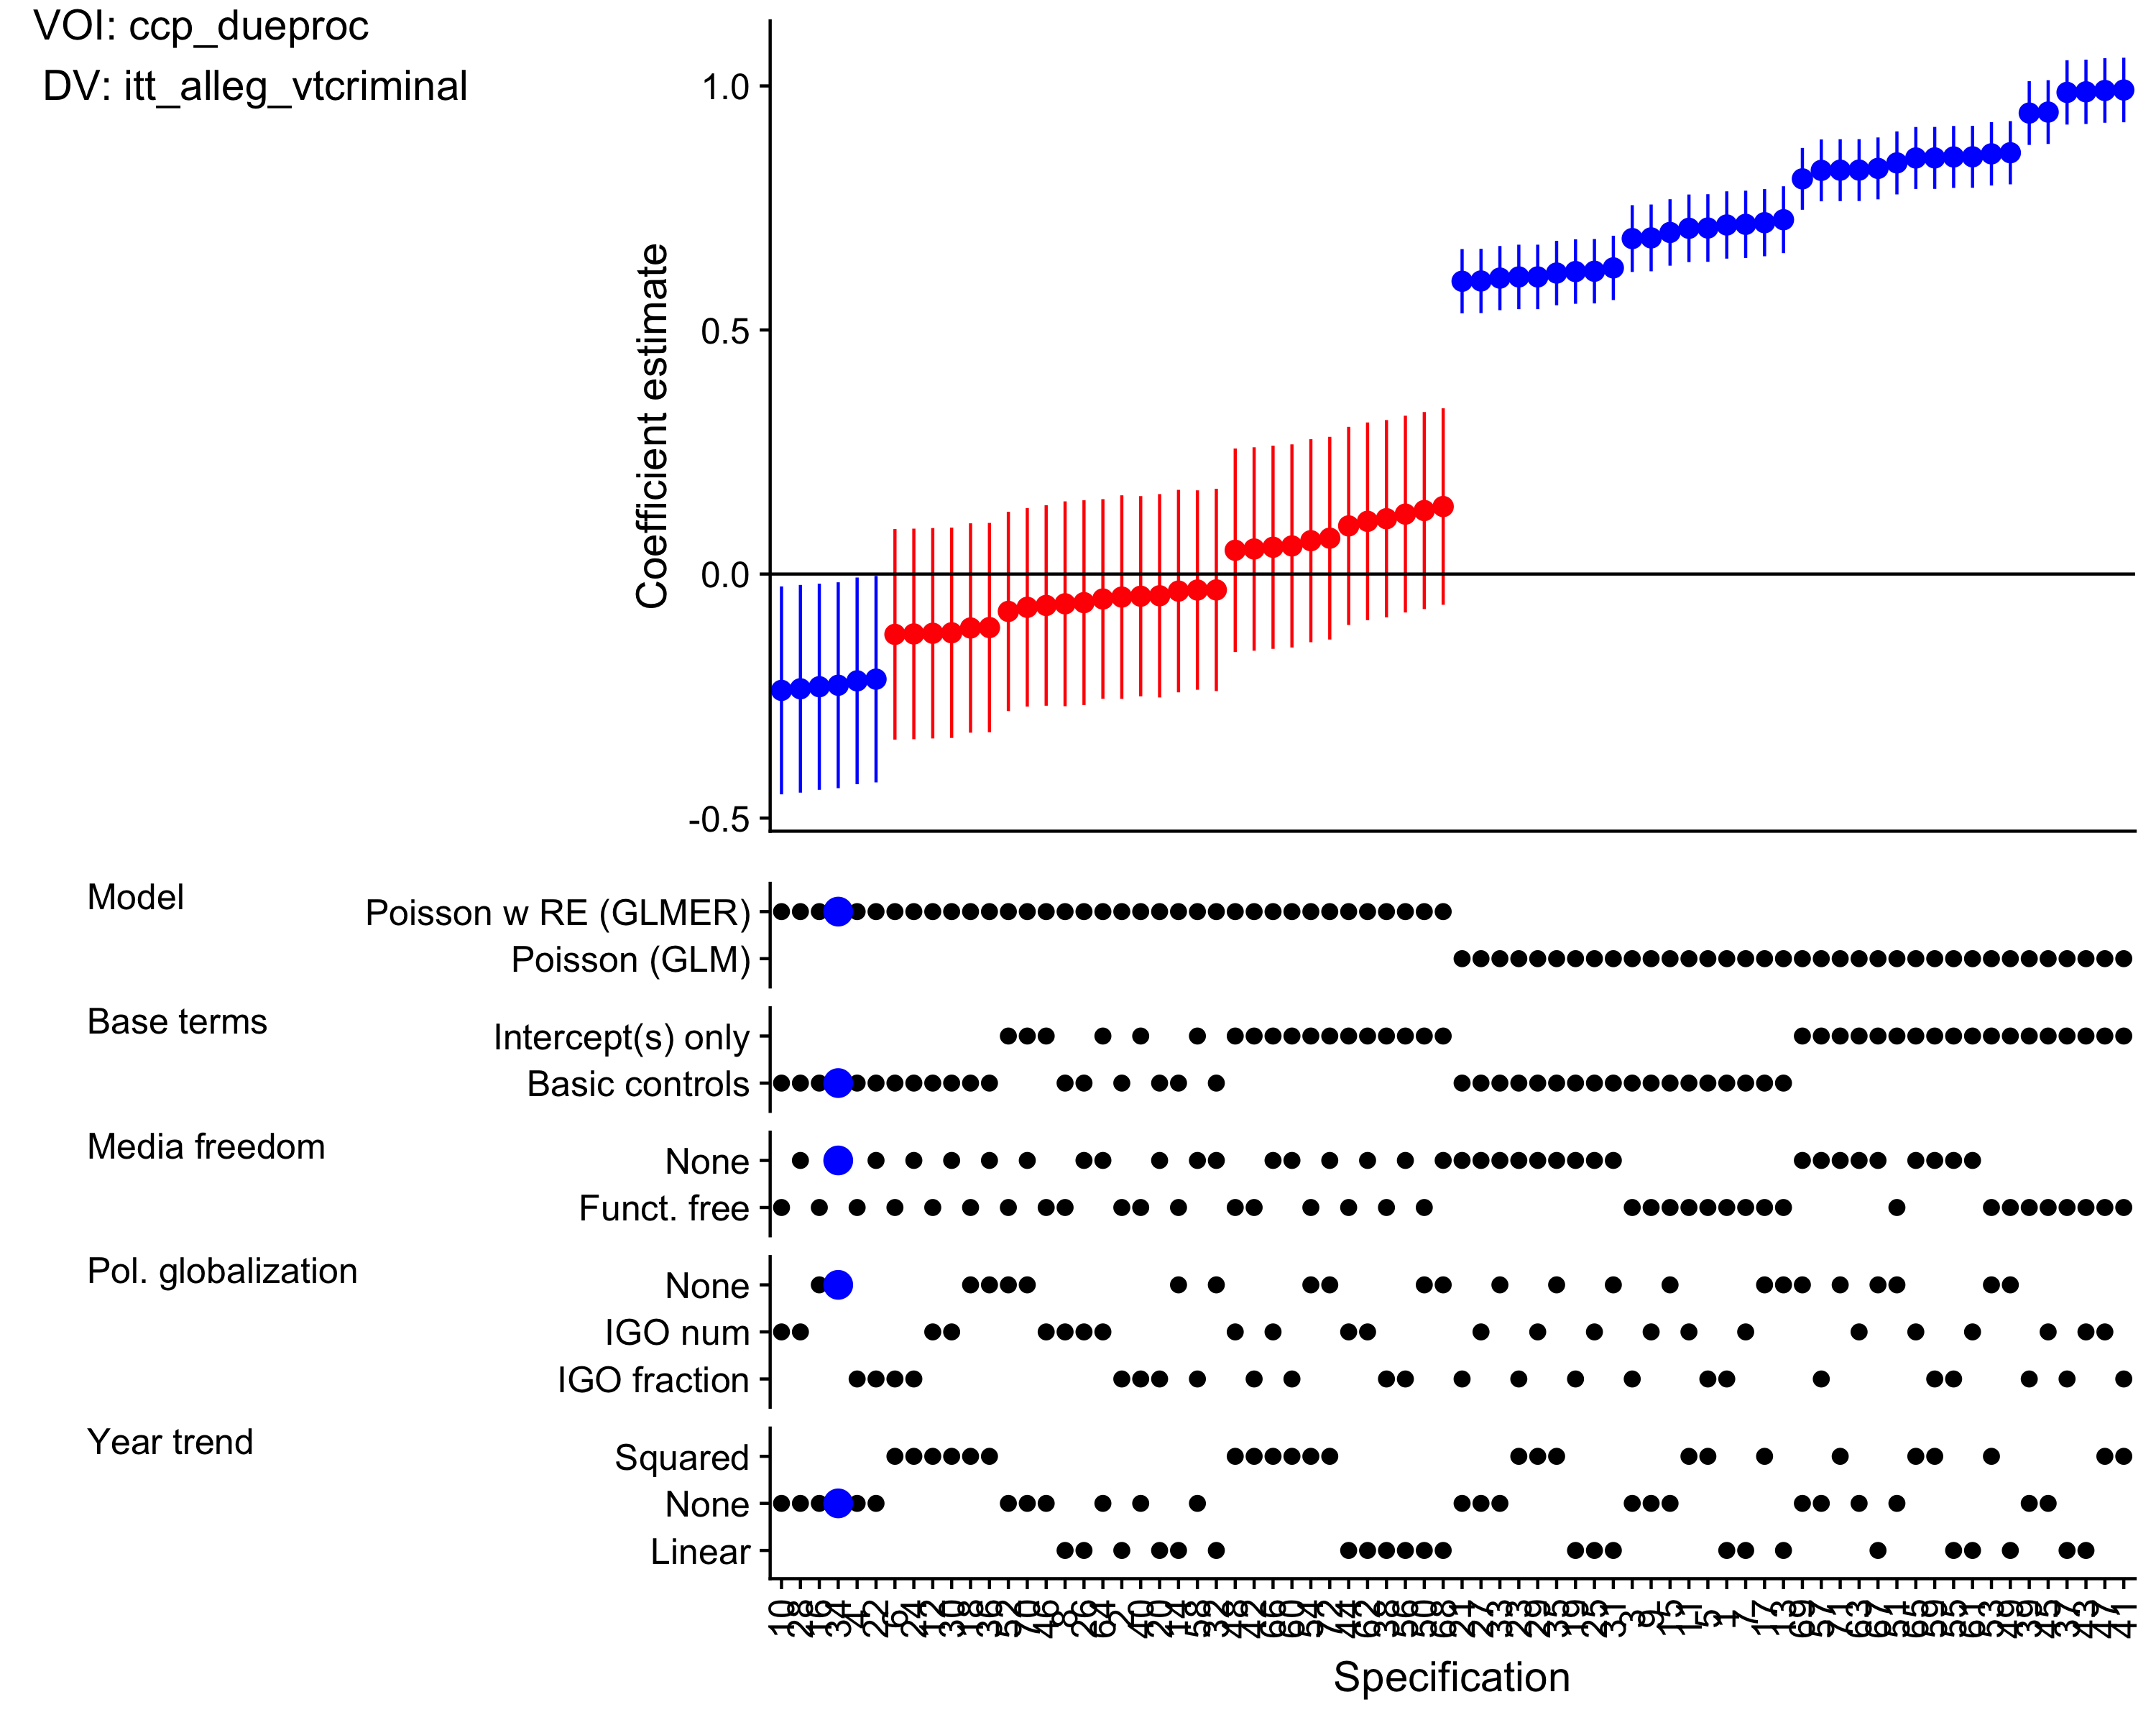
\includegraphics{../output/figures-robustness/specplot-ccp_dueproc-itt_alleg_vtcriminal.png}

\hypertarget{list-of-all-specification-plots}{%
\section{List of all specification
plots}\label{list-of-all-specification-plots}}

\hypertarget{voi-ccp_dueproc}{%
\subsection{VOI: ccp\_dueproc}\label{voi-ccp_dueproc}}

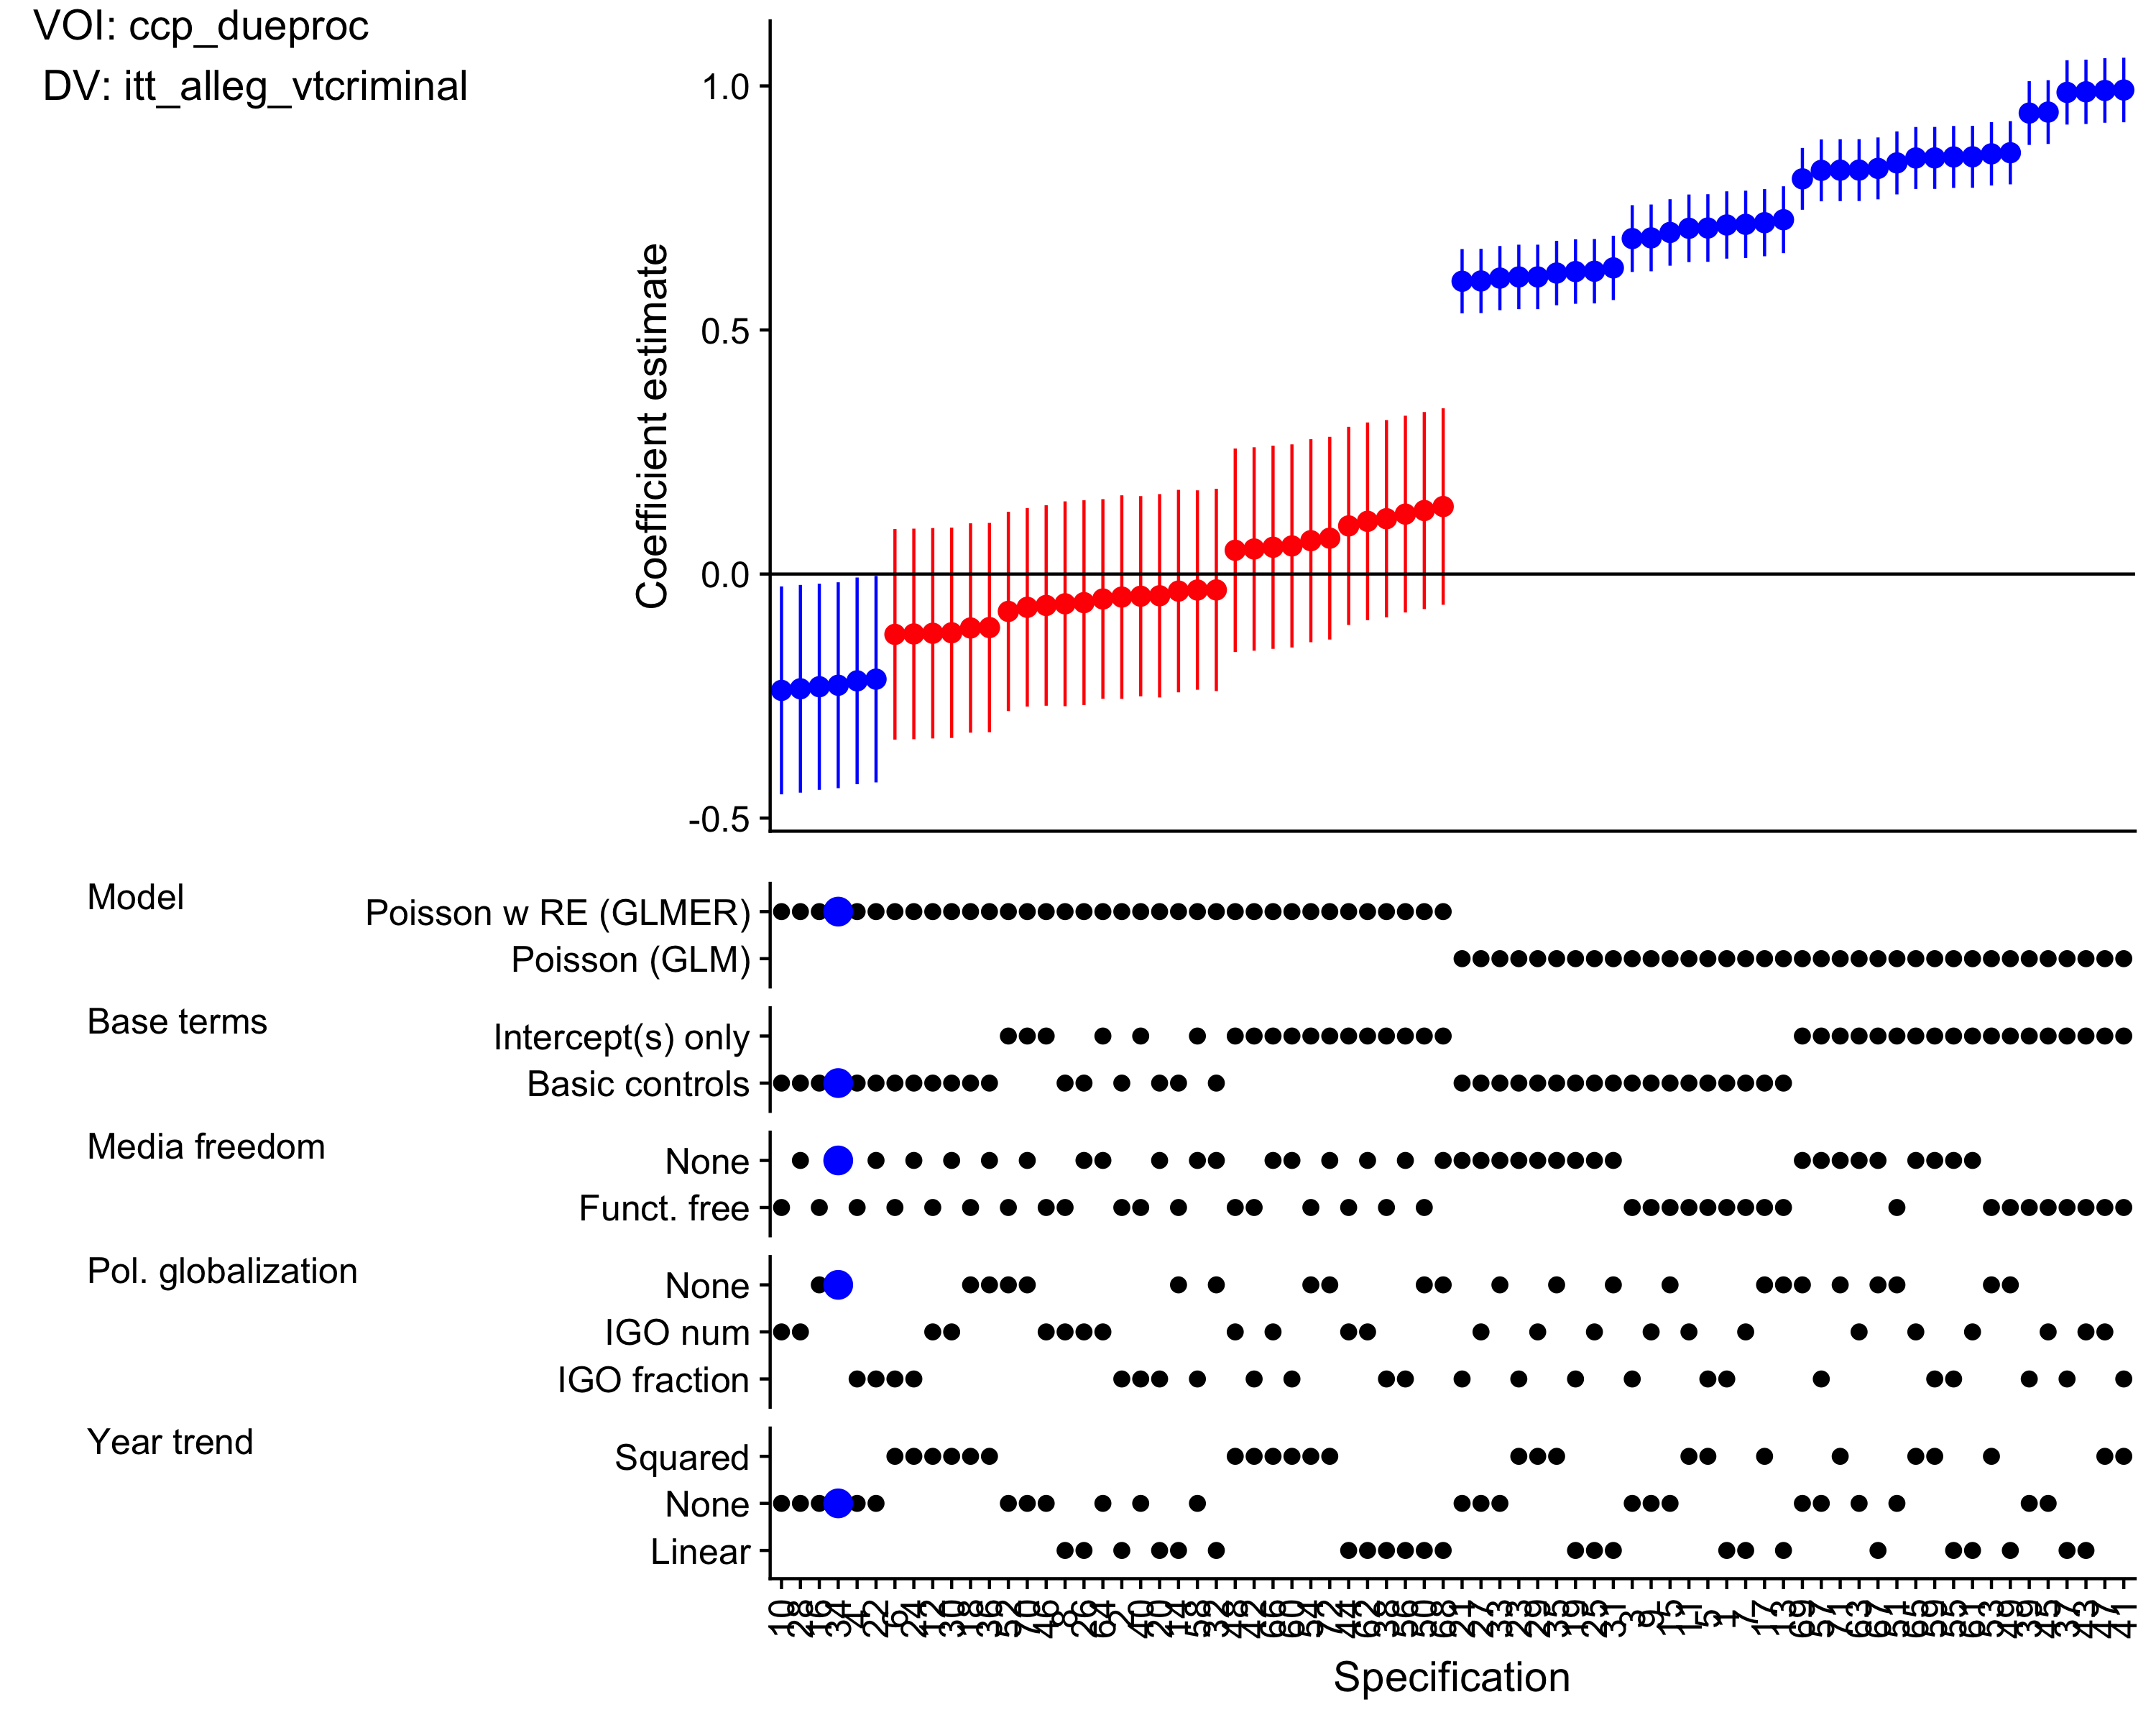
\includegraphics[height=4in]{../output/figures-robustness/specplot-ccp_dueproc-itt_alleg_vtcriminal.png}

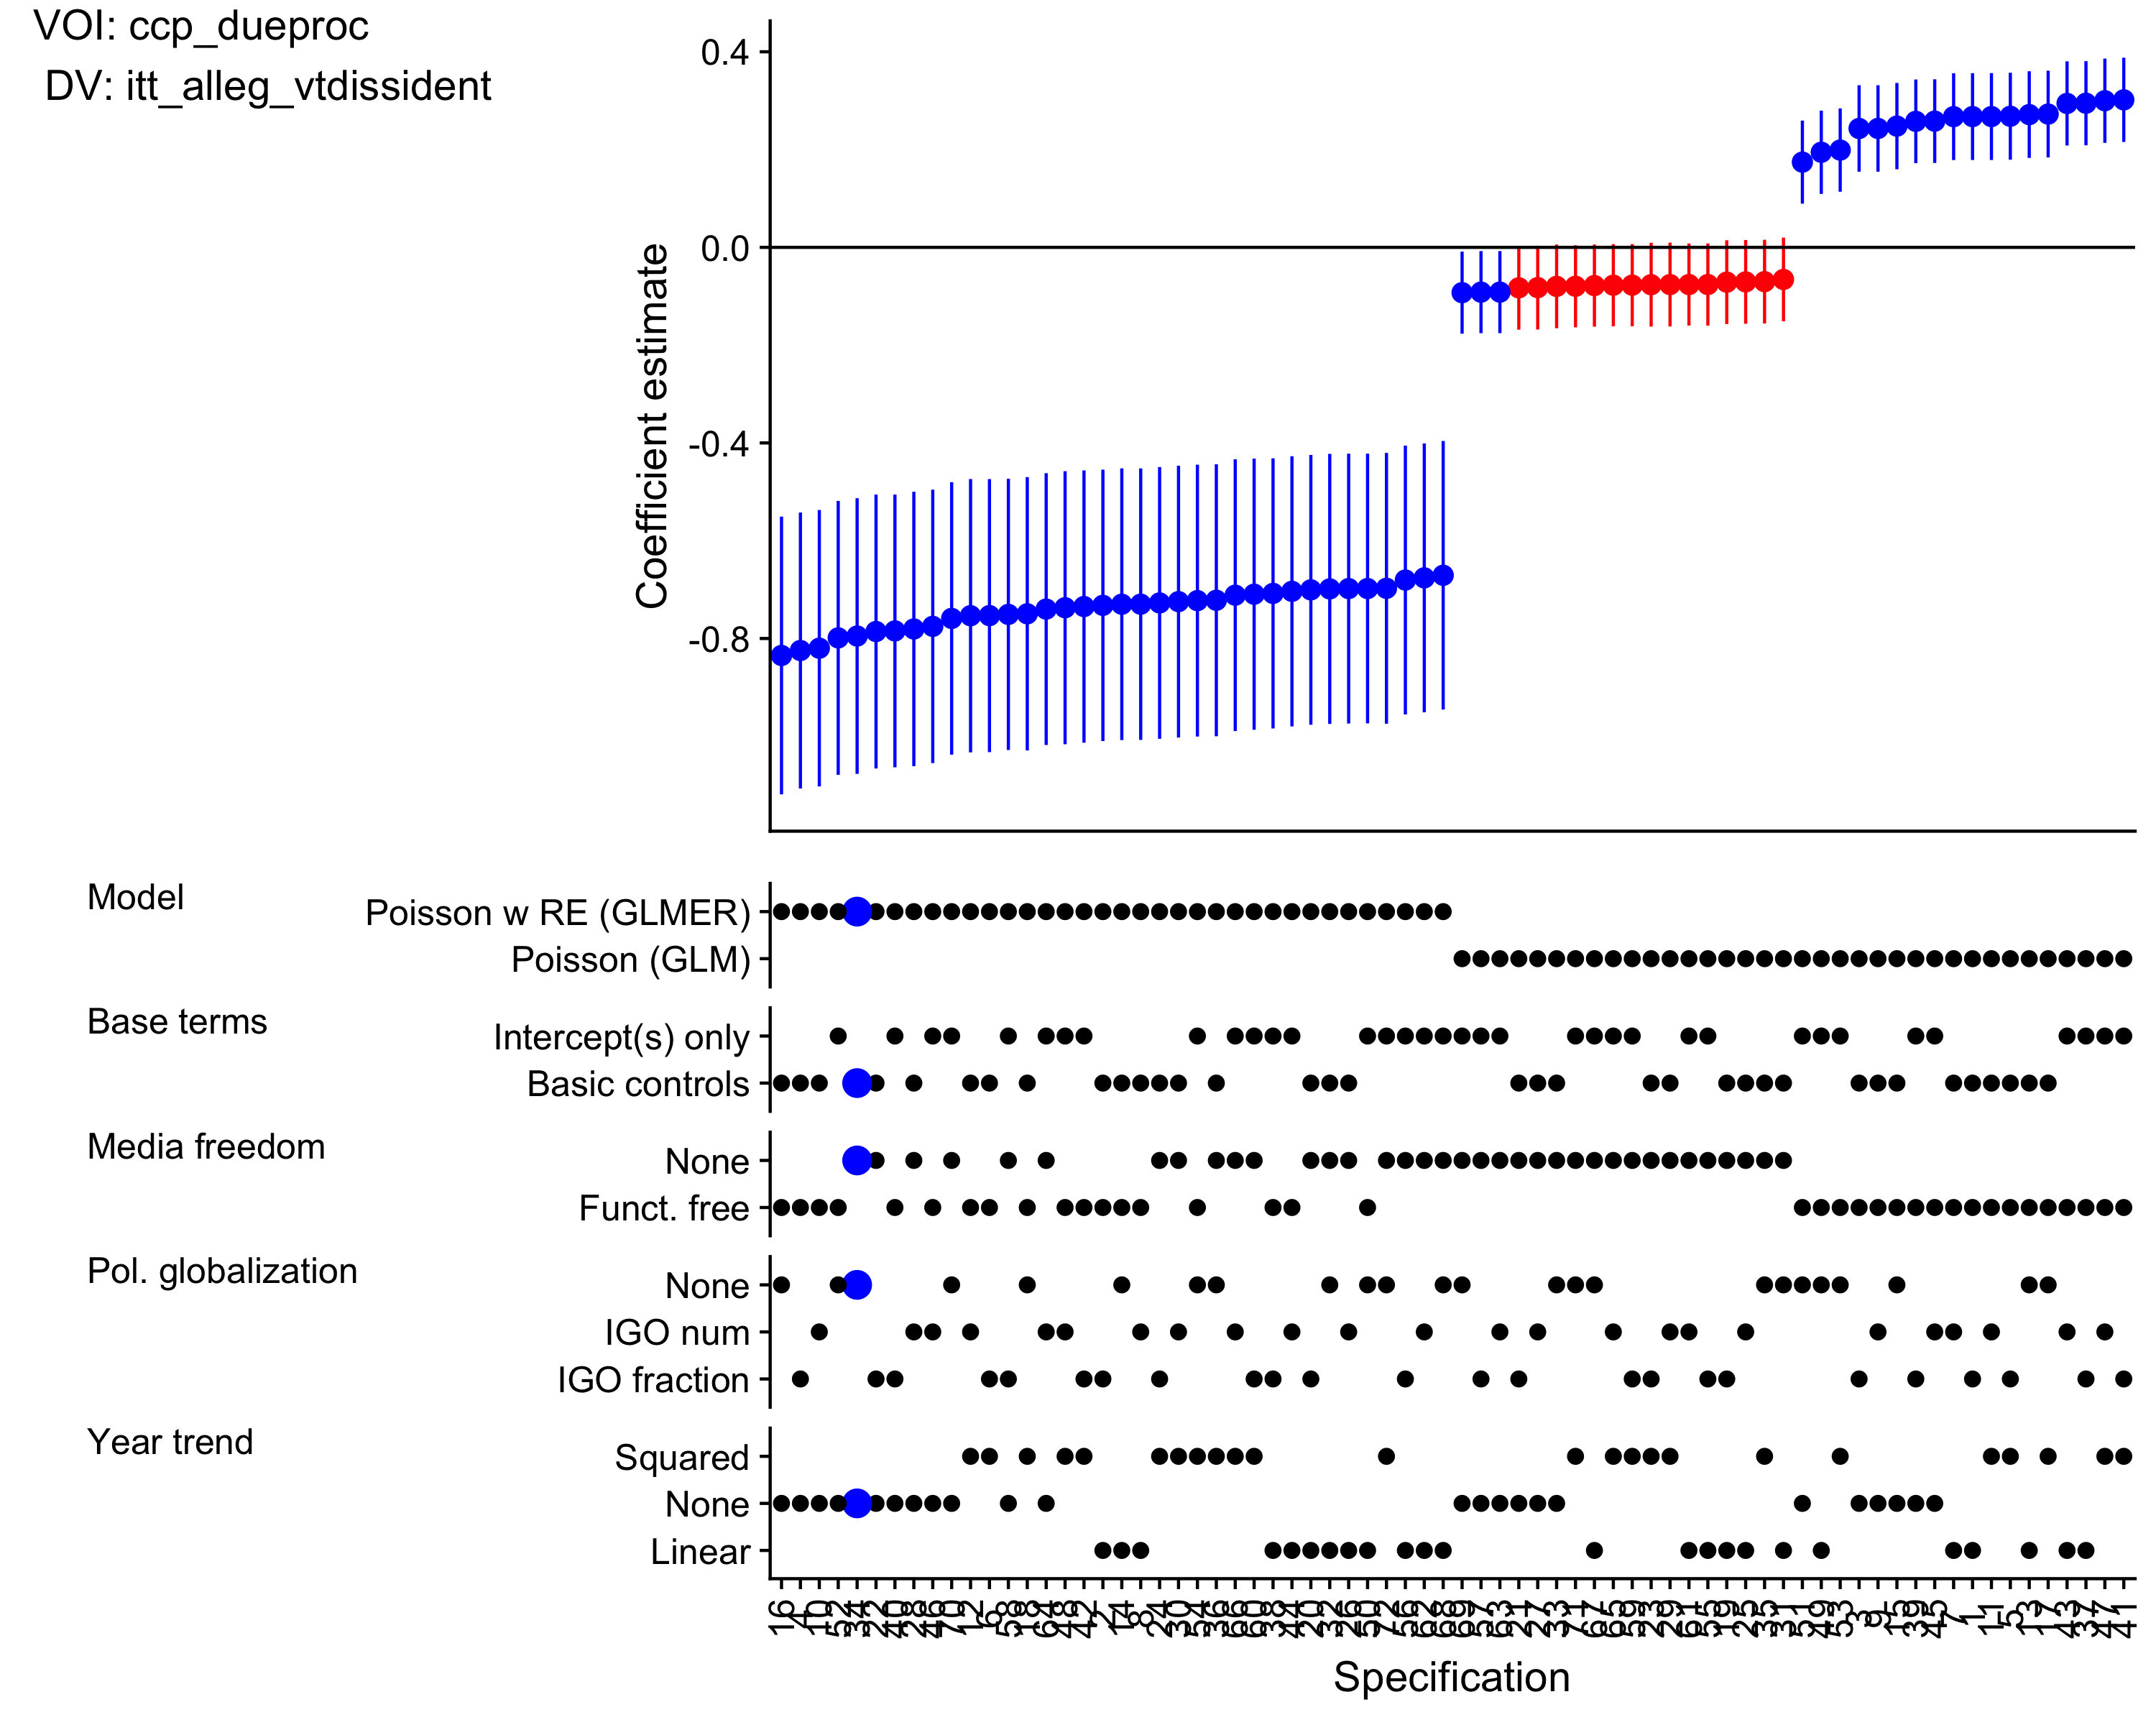
\includegraphics[height=4in]{../output/figures-robustness/specplot-ccp_dueproc-itt_alleg_vtdissident.png}

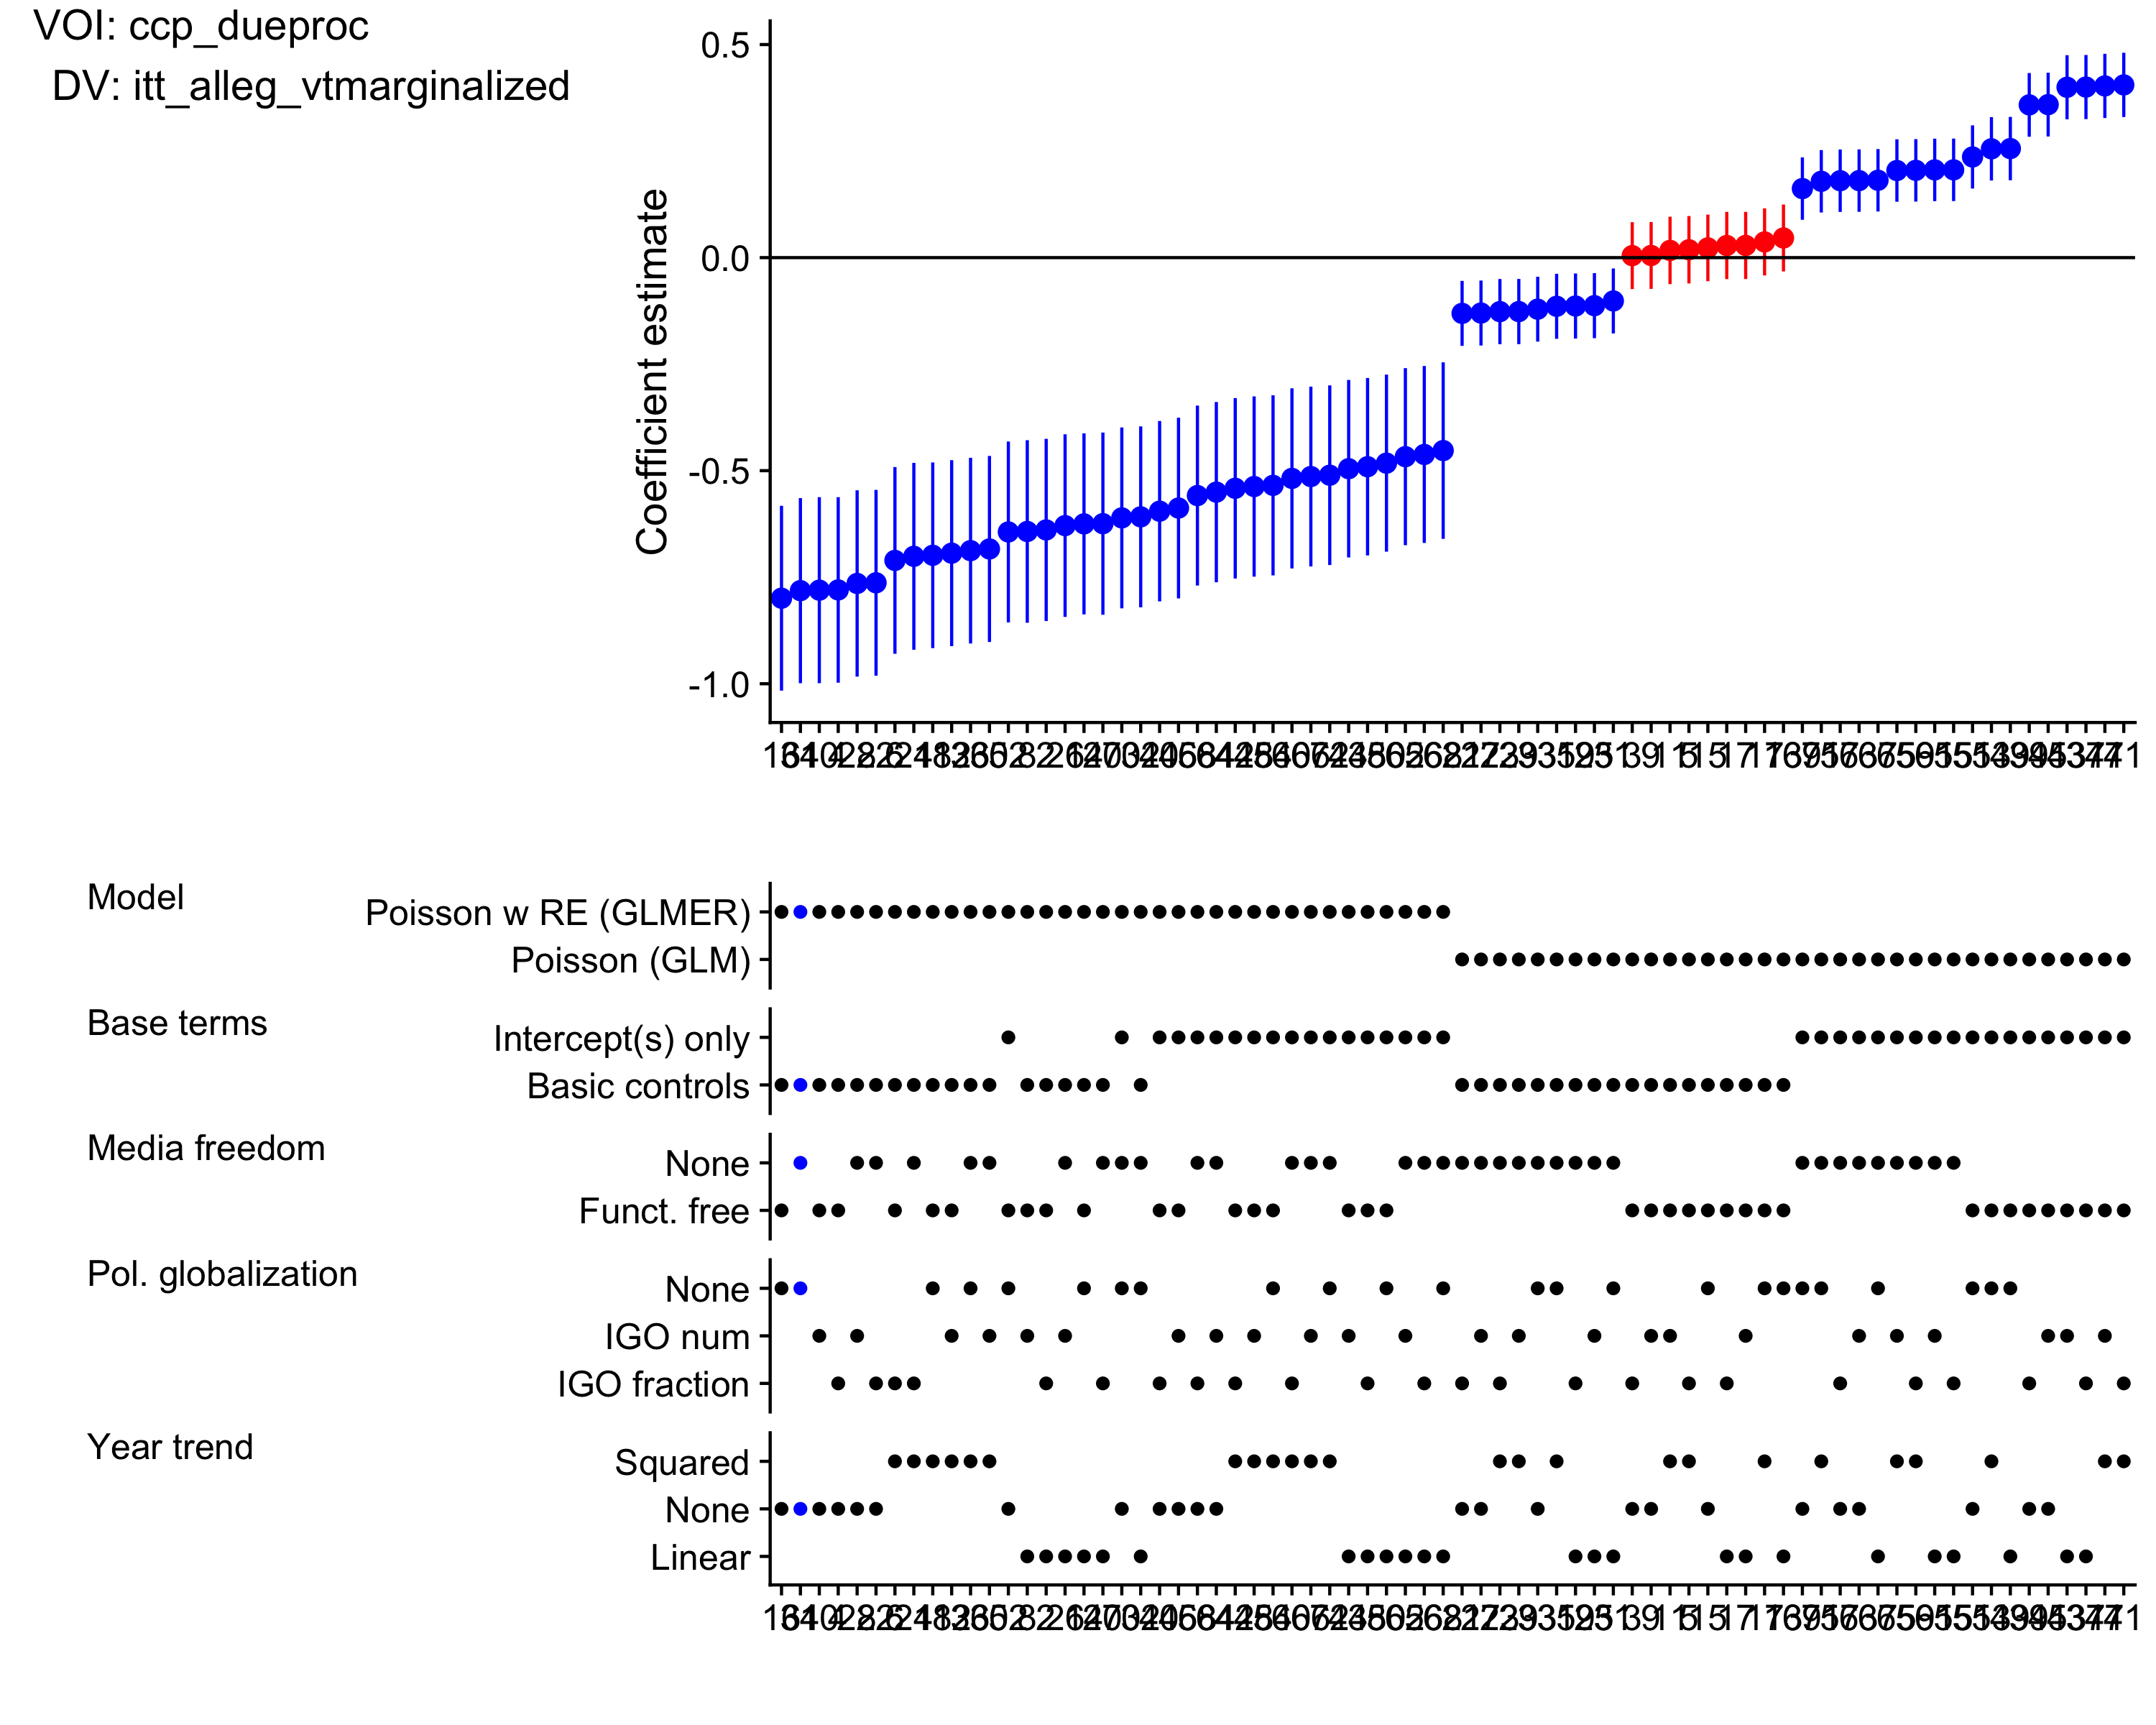
\includegraphics[height=4in]{../output/figures-robustness/specplot-ccp_dueproc-itt_alleg_vtmarginalized.png}

\hypertarget{voi-ccp_habcorp}{%
\subsection{VOI: ccp\_habcorp}\label{voi-ccp_habcorp}}

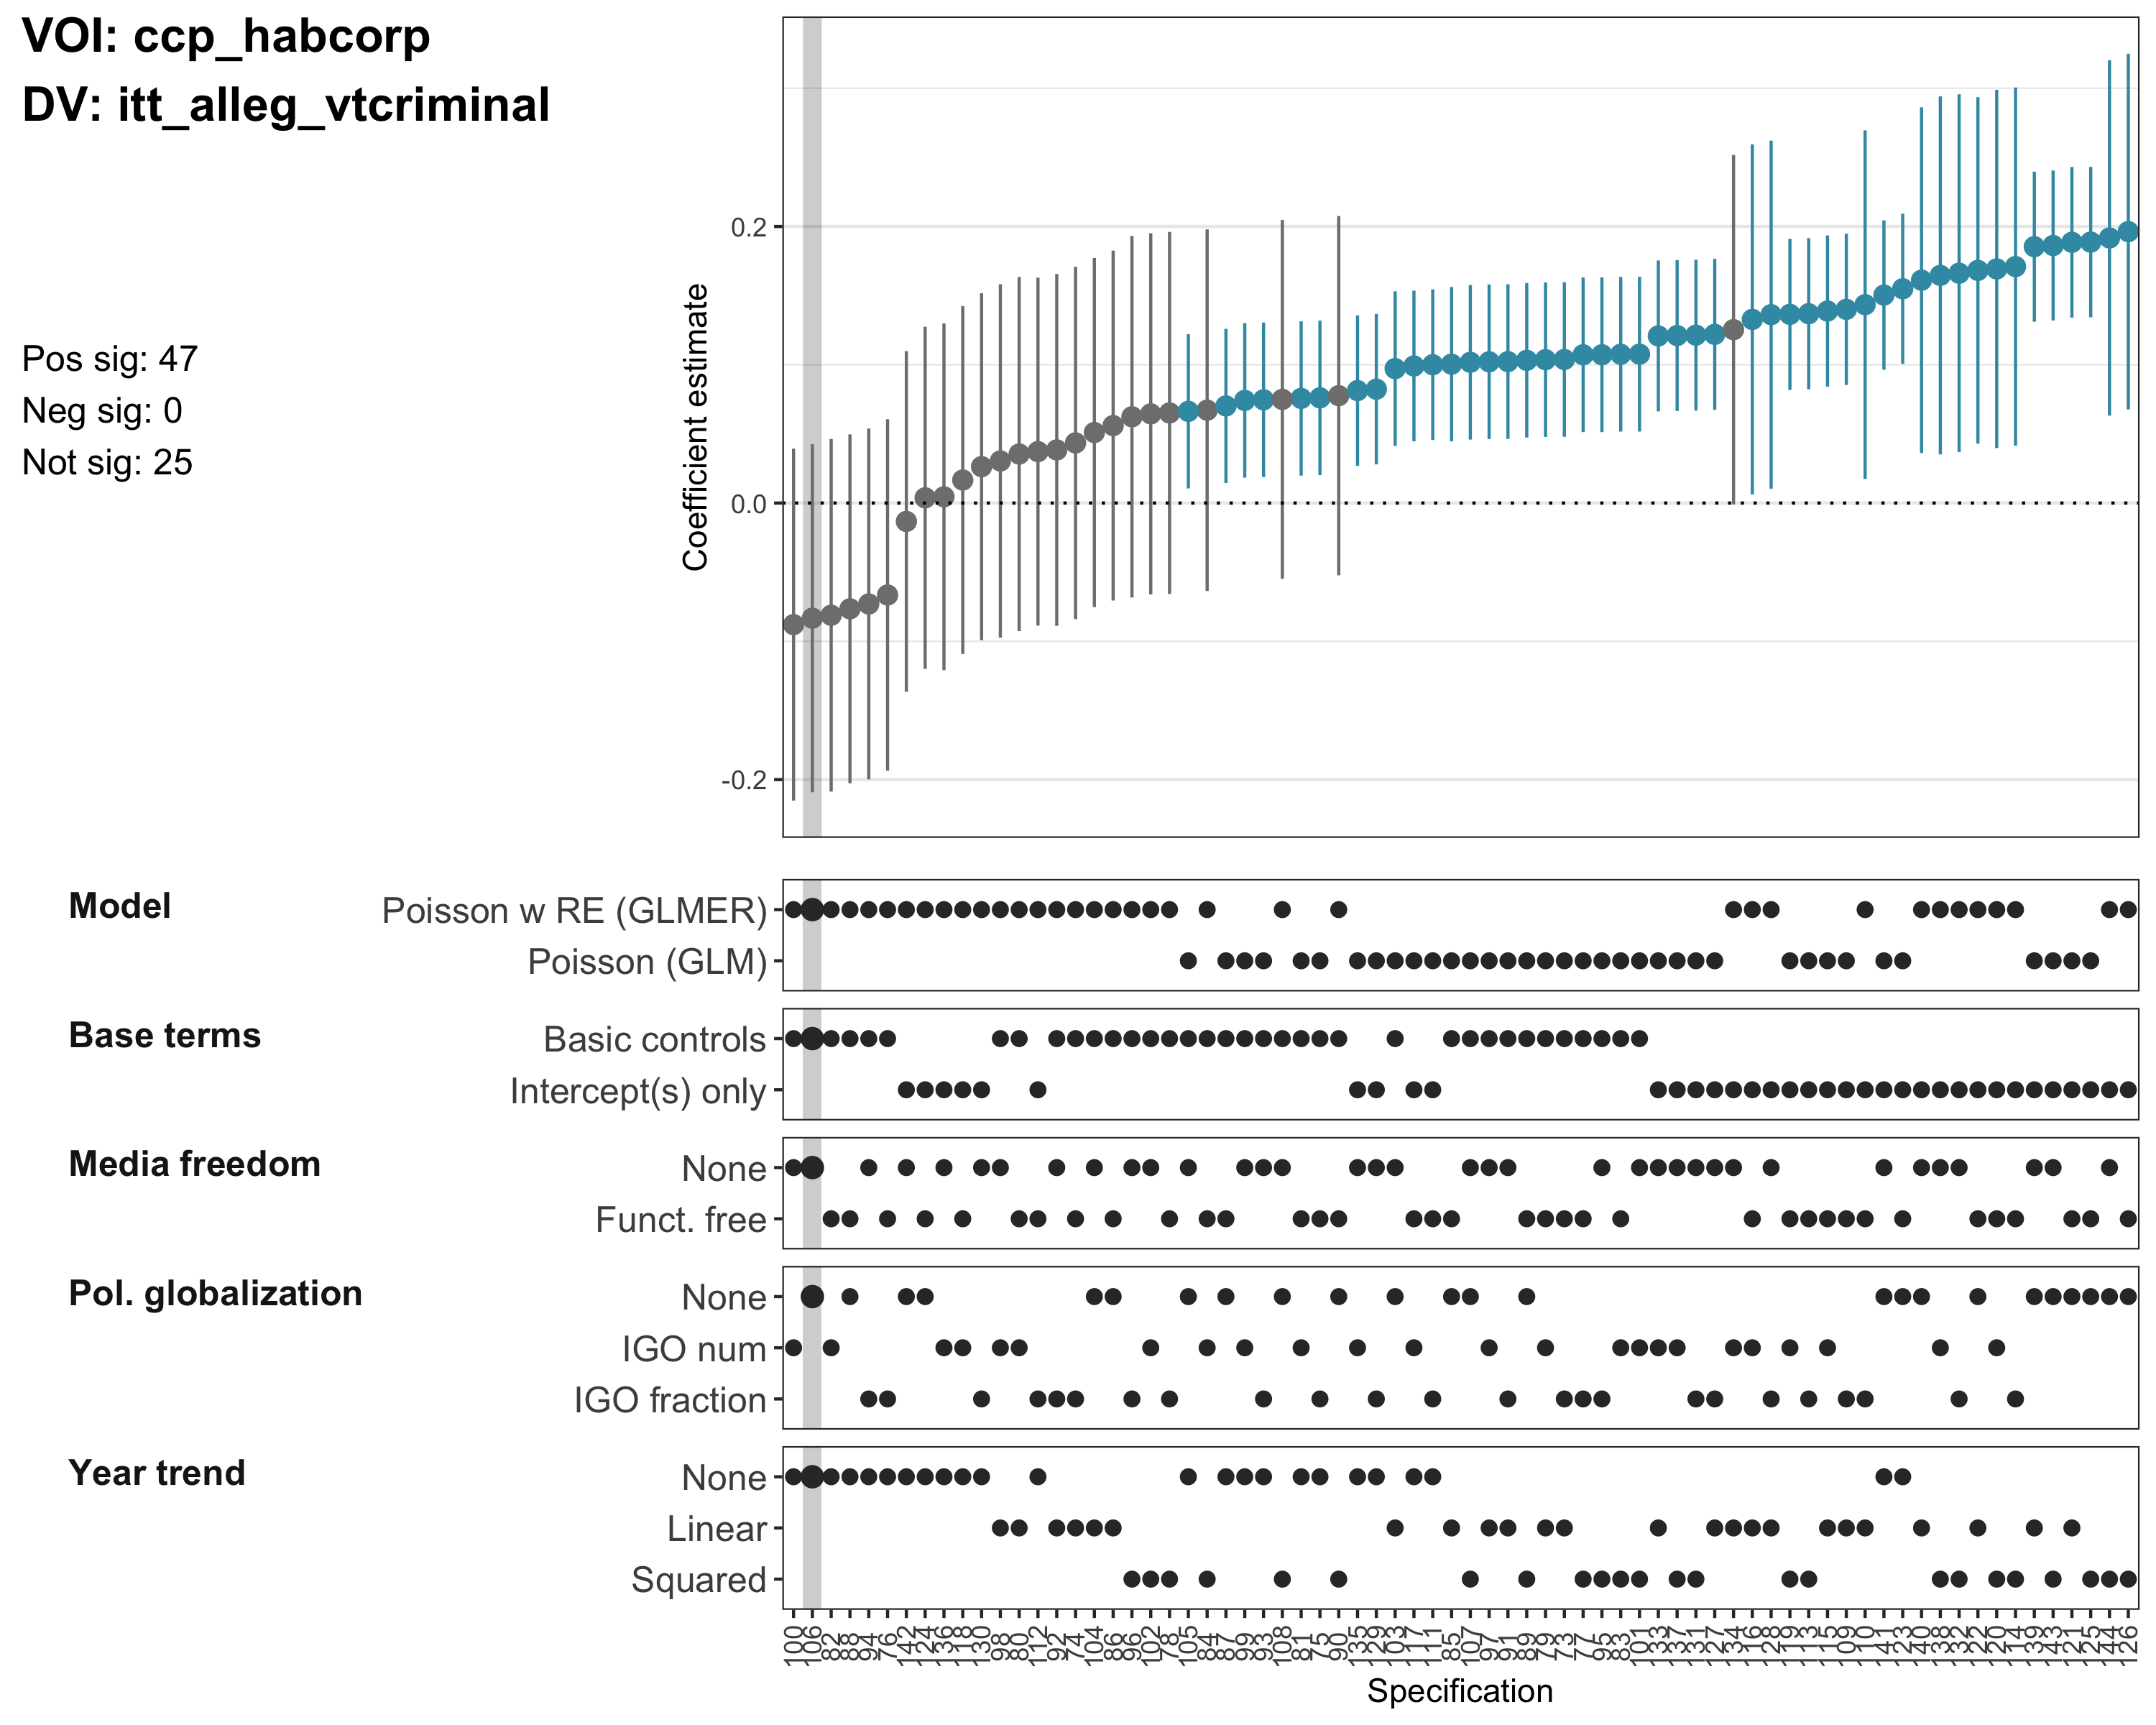
\includegraphics[height=4in]{../output/figures-robustness/specplot-ccp_habcorp-itt_alleg_vtcriminal.png}

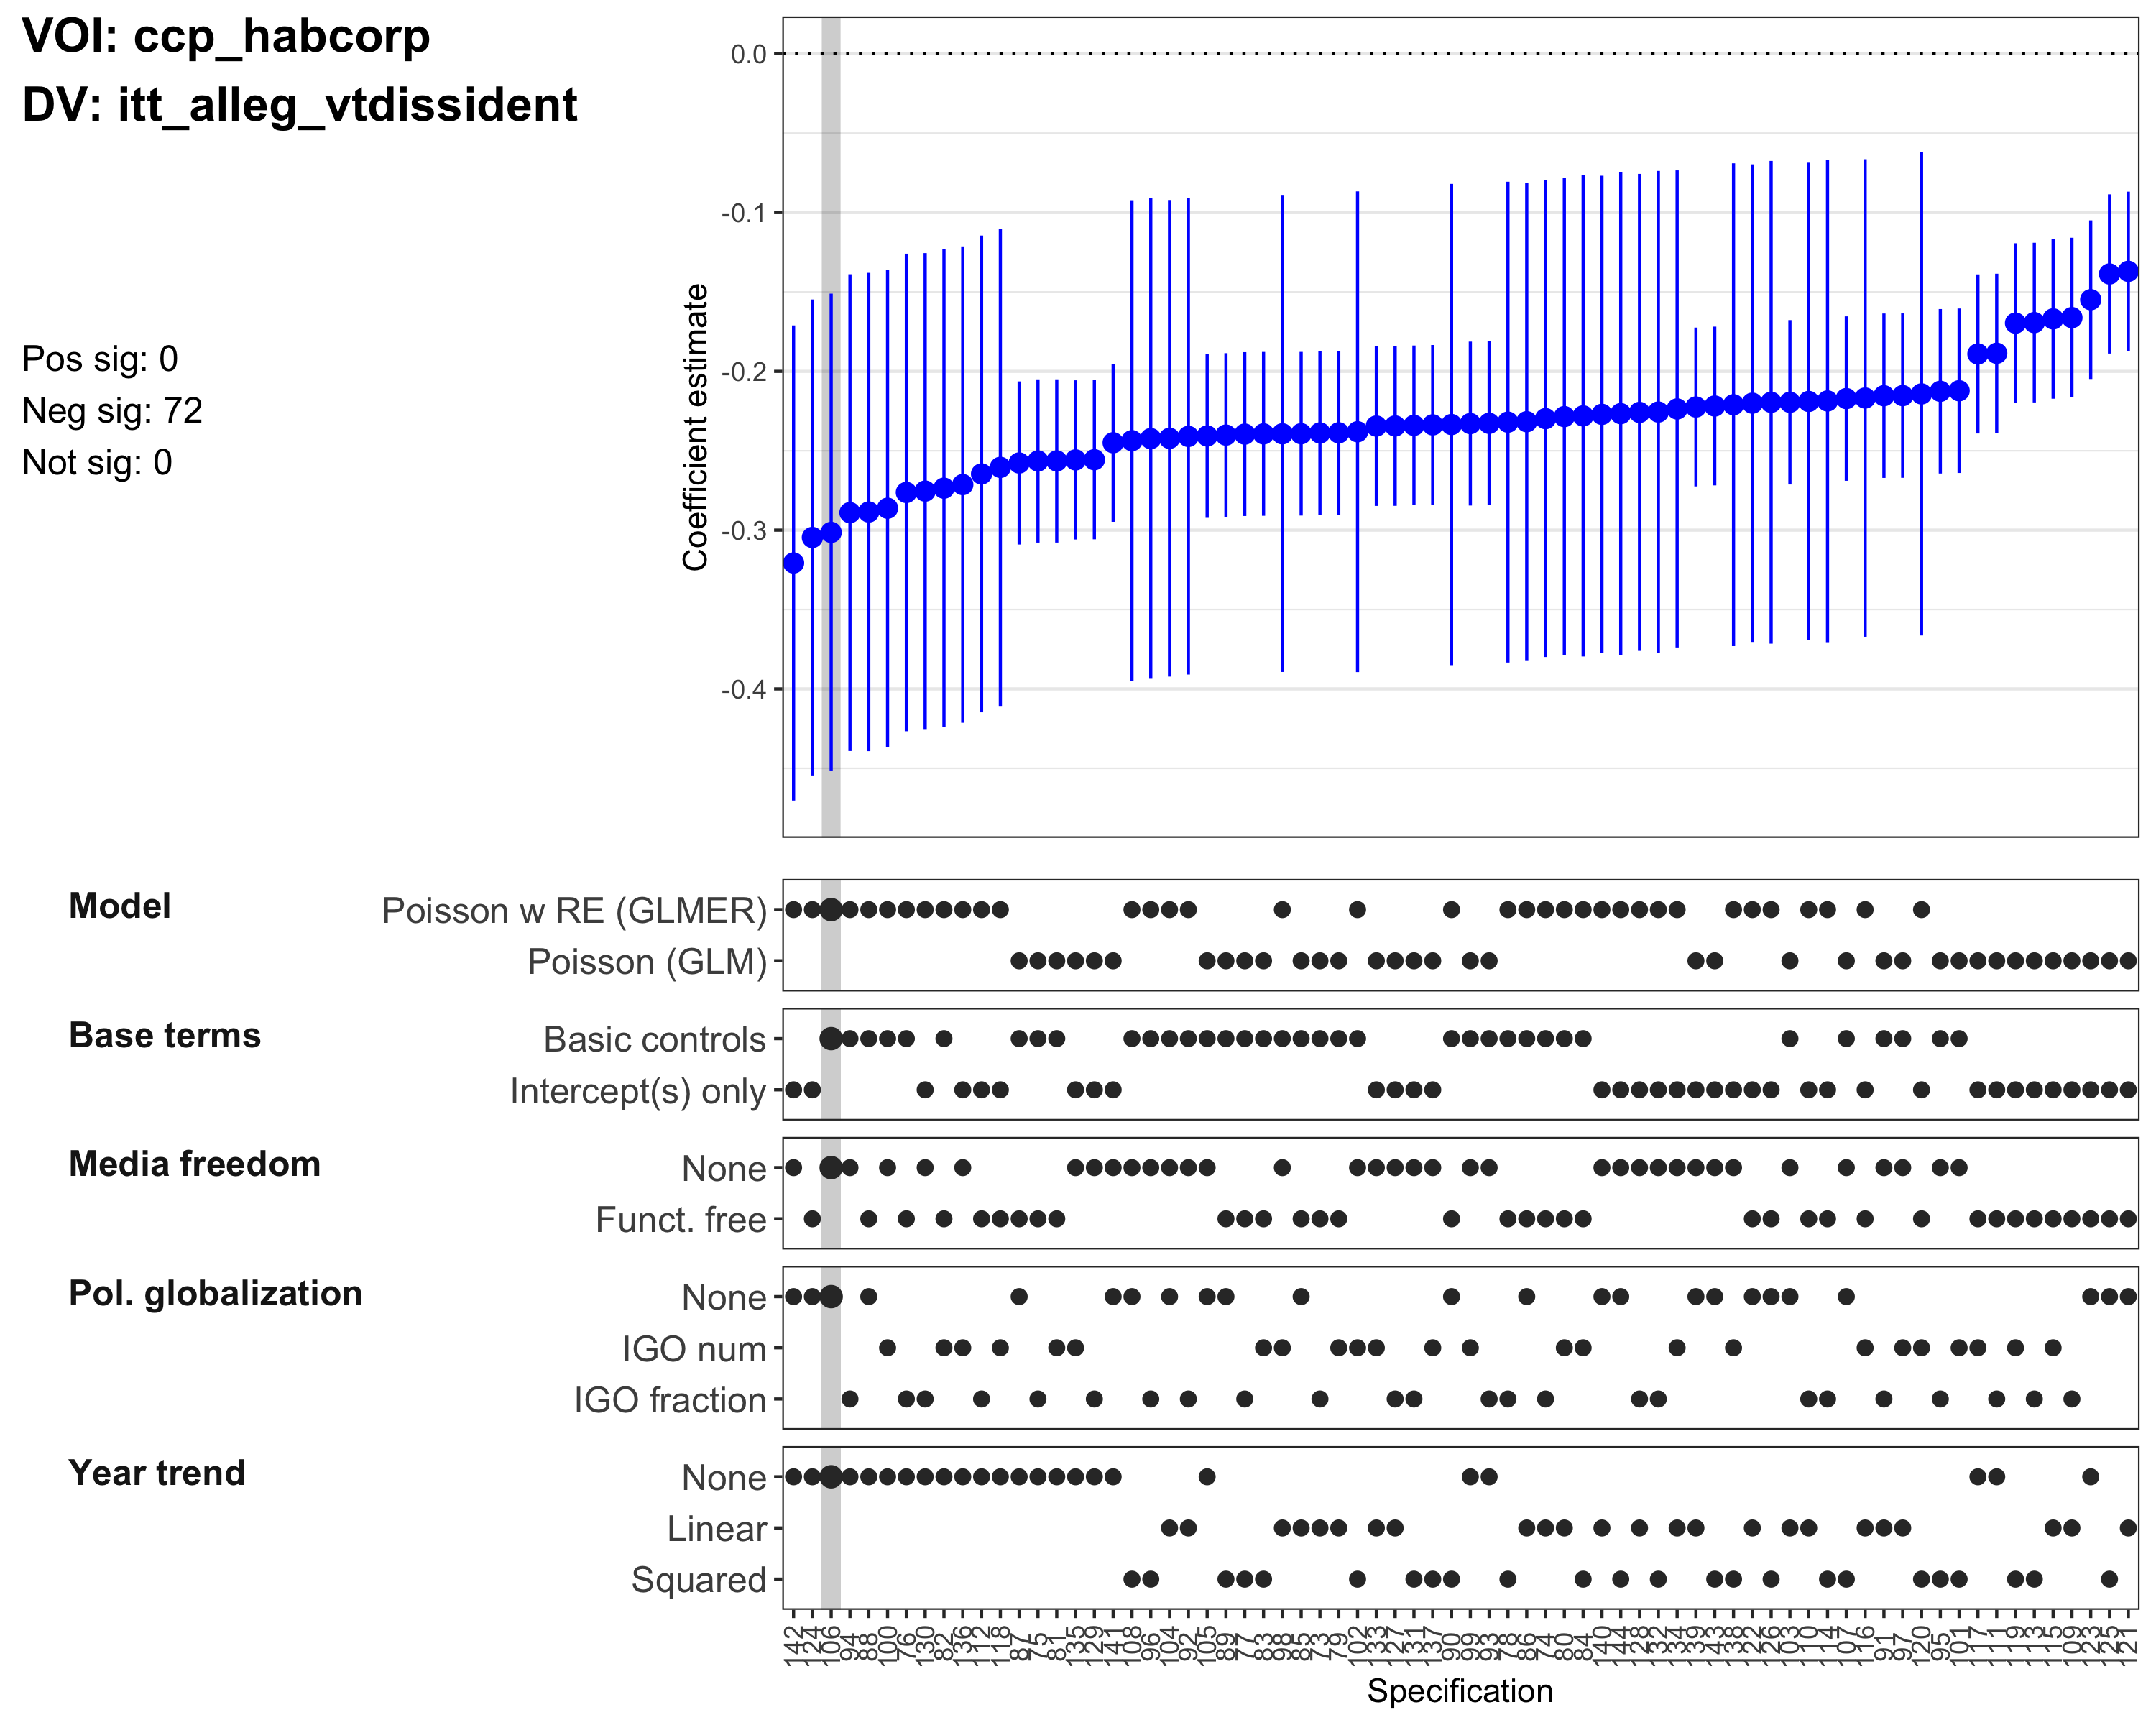
\includegraphics[height=4in]{../output/figures-robustness/specplot-ccp_habcorp-itt_alleg_vtdissident.png}

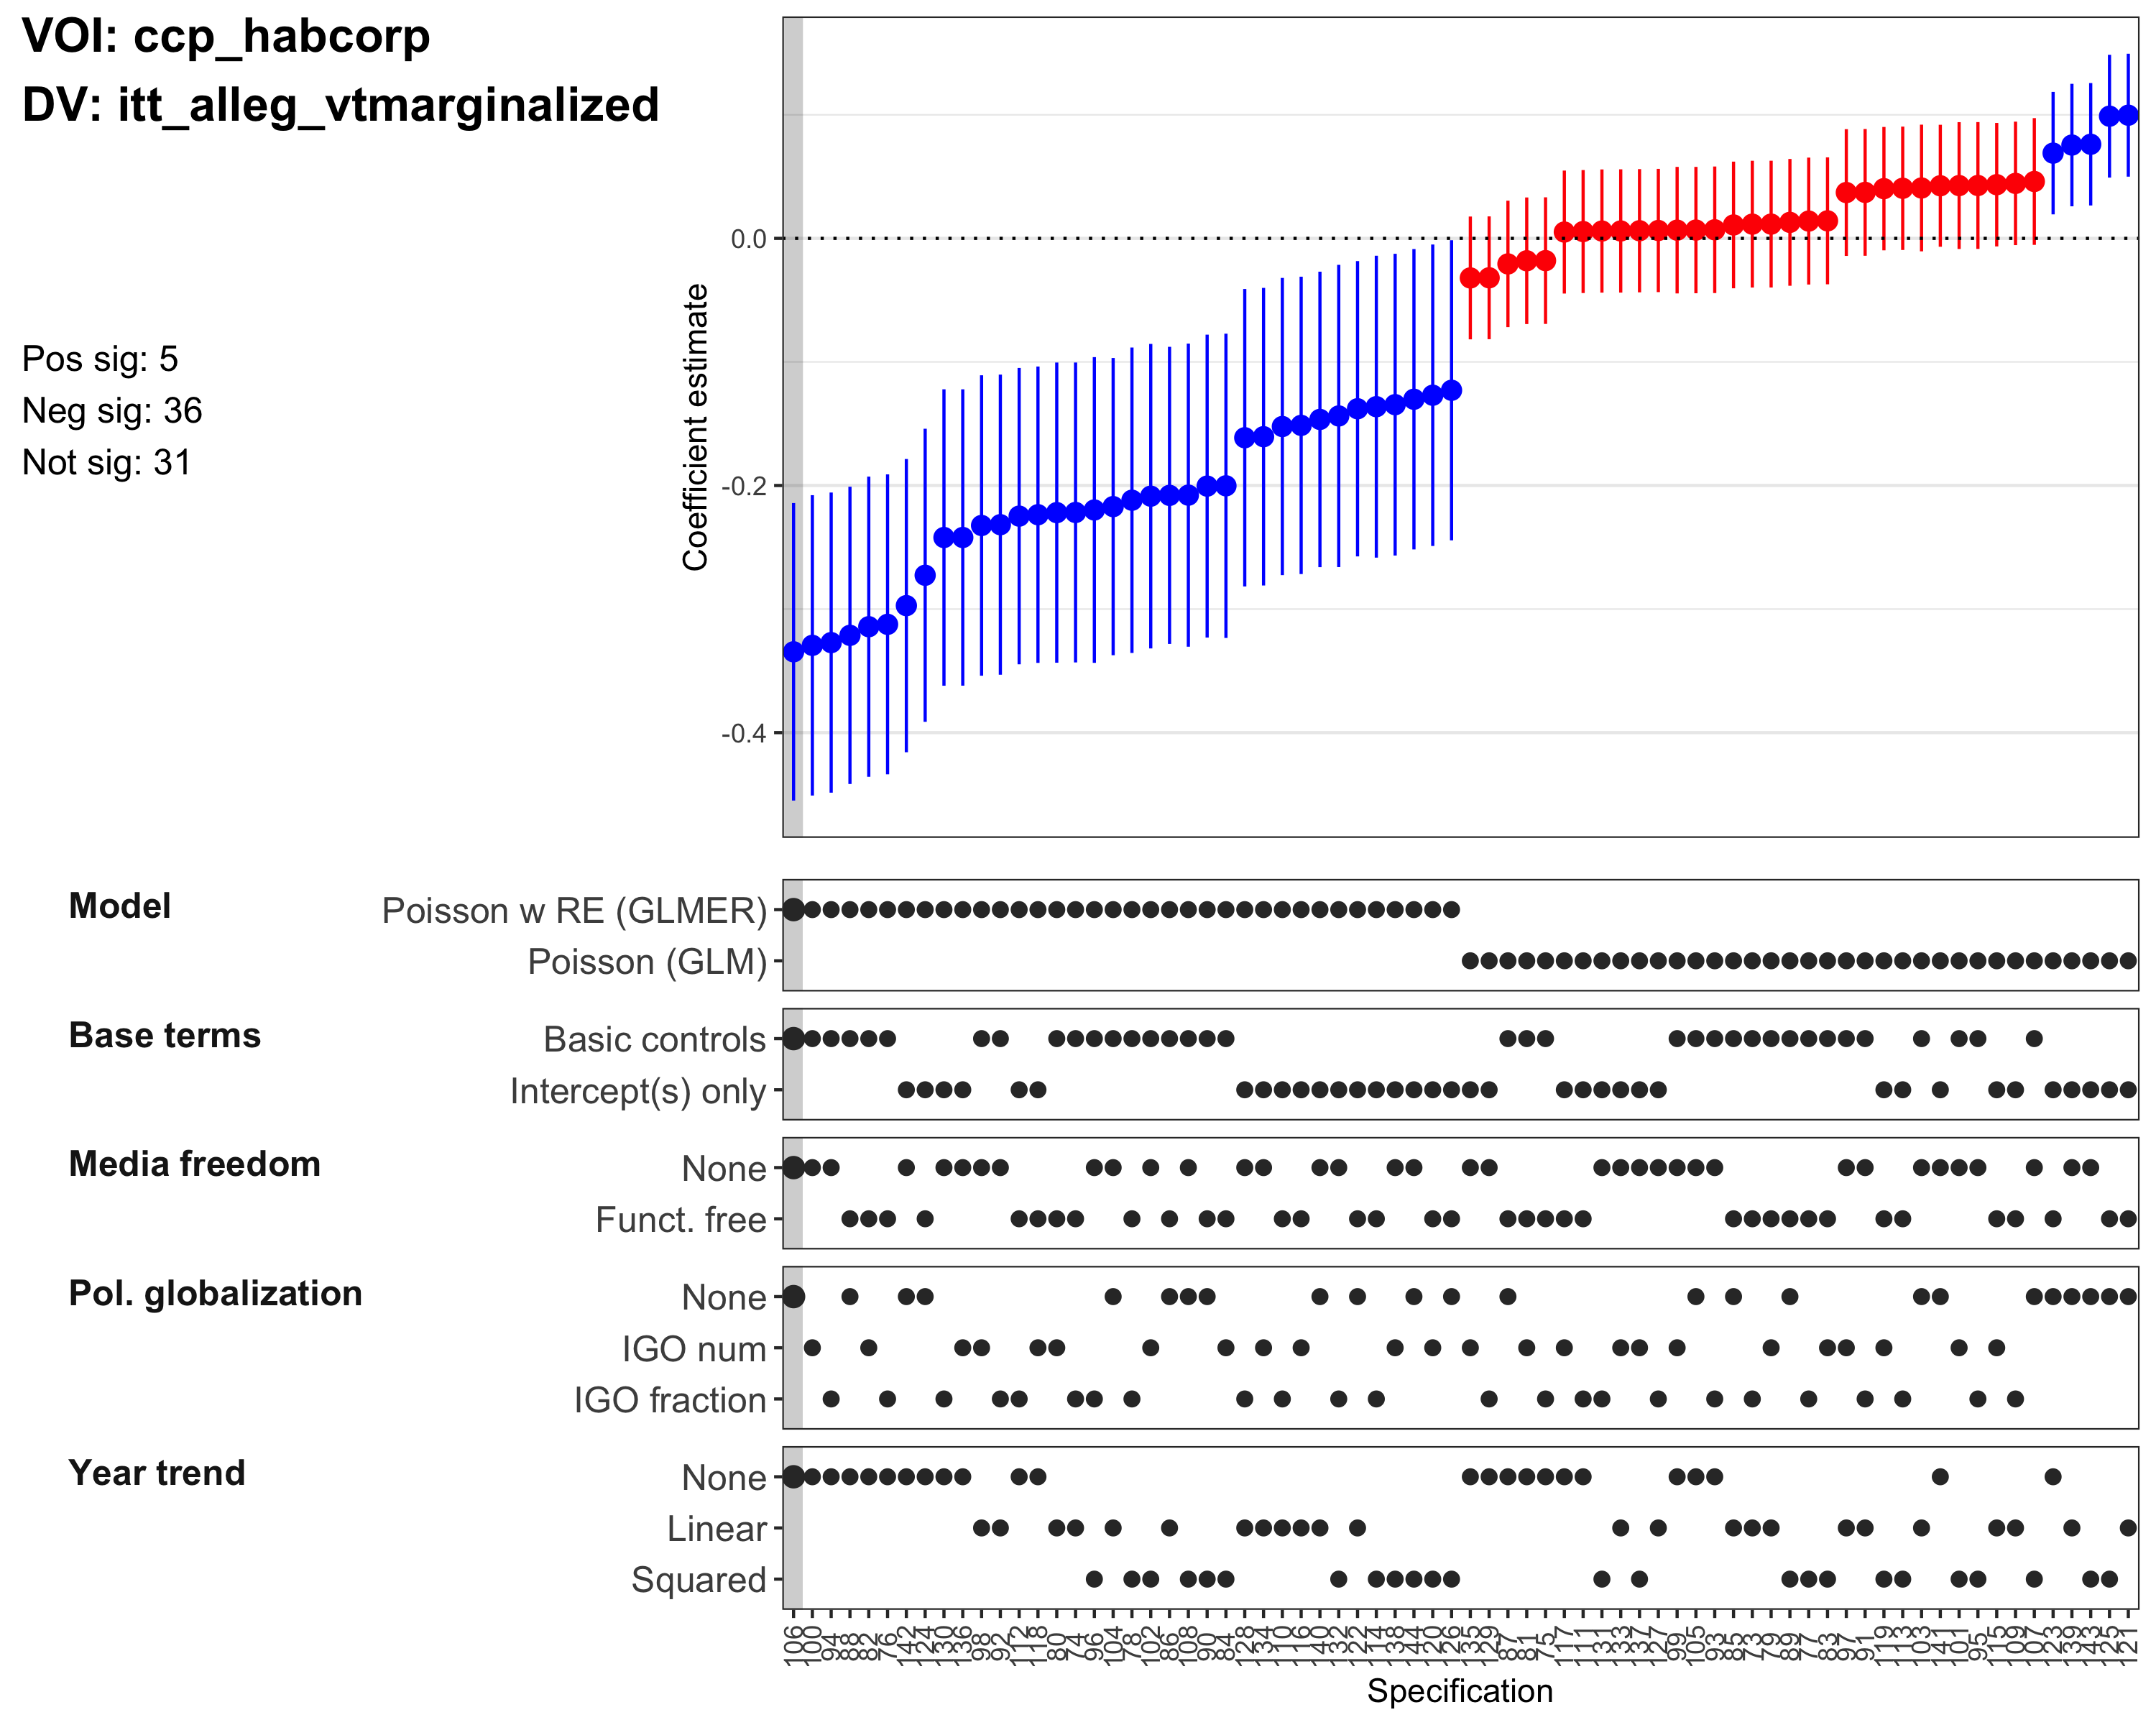
\includegraphics[height=4in]{../output/figures-robustness/specplot-ccp_habcorp-itt_alleg_vtmarginalized.png}

\hypertarget{voi-ccp_prerel}{%
\subsection{VOI: ccp\_prerel}\label{voi-ccp_prerel}}

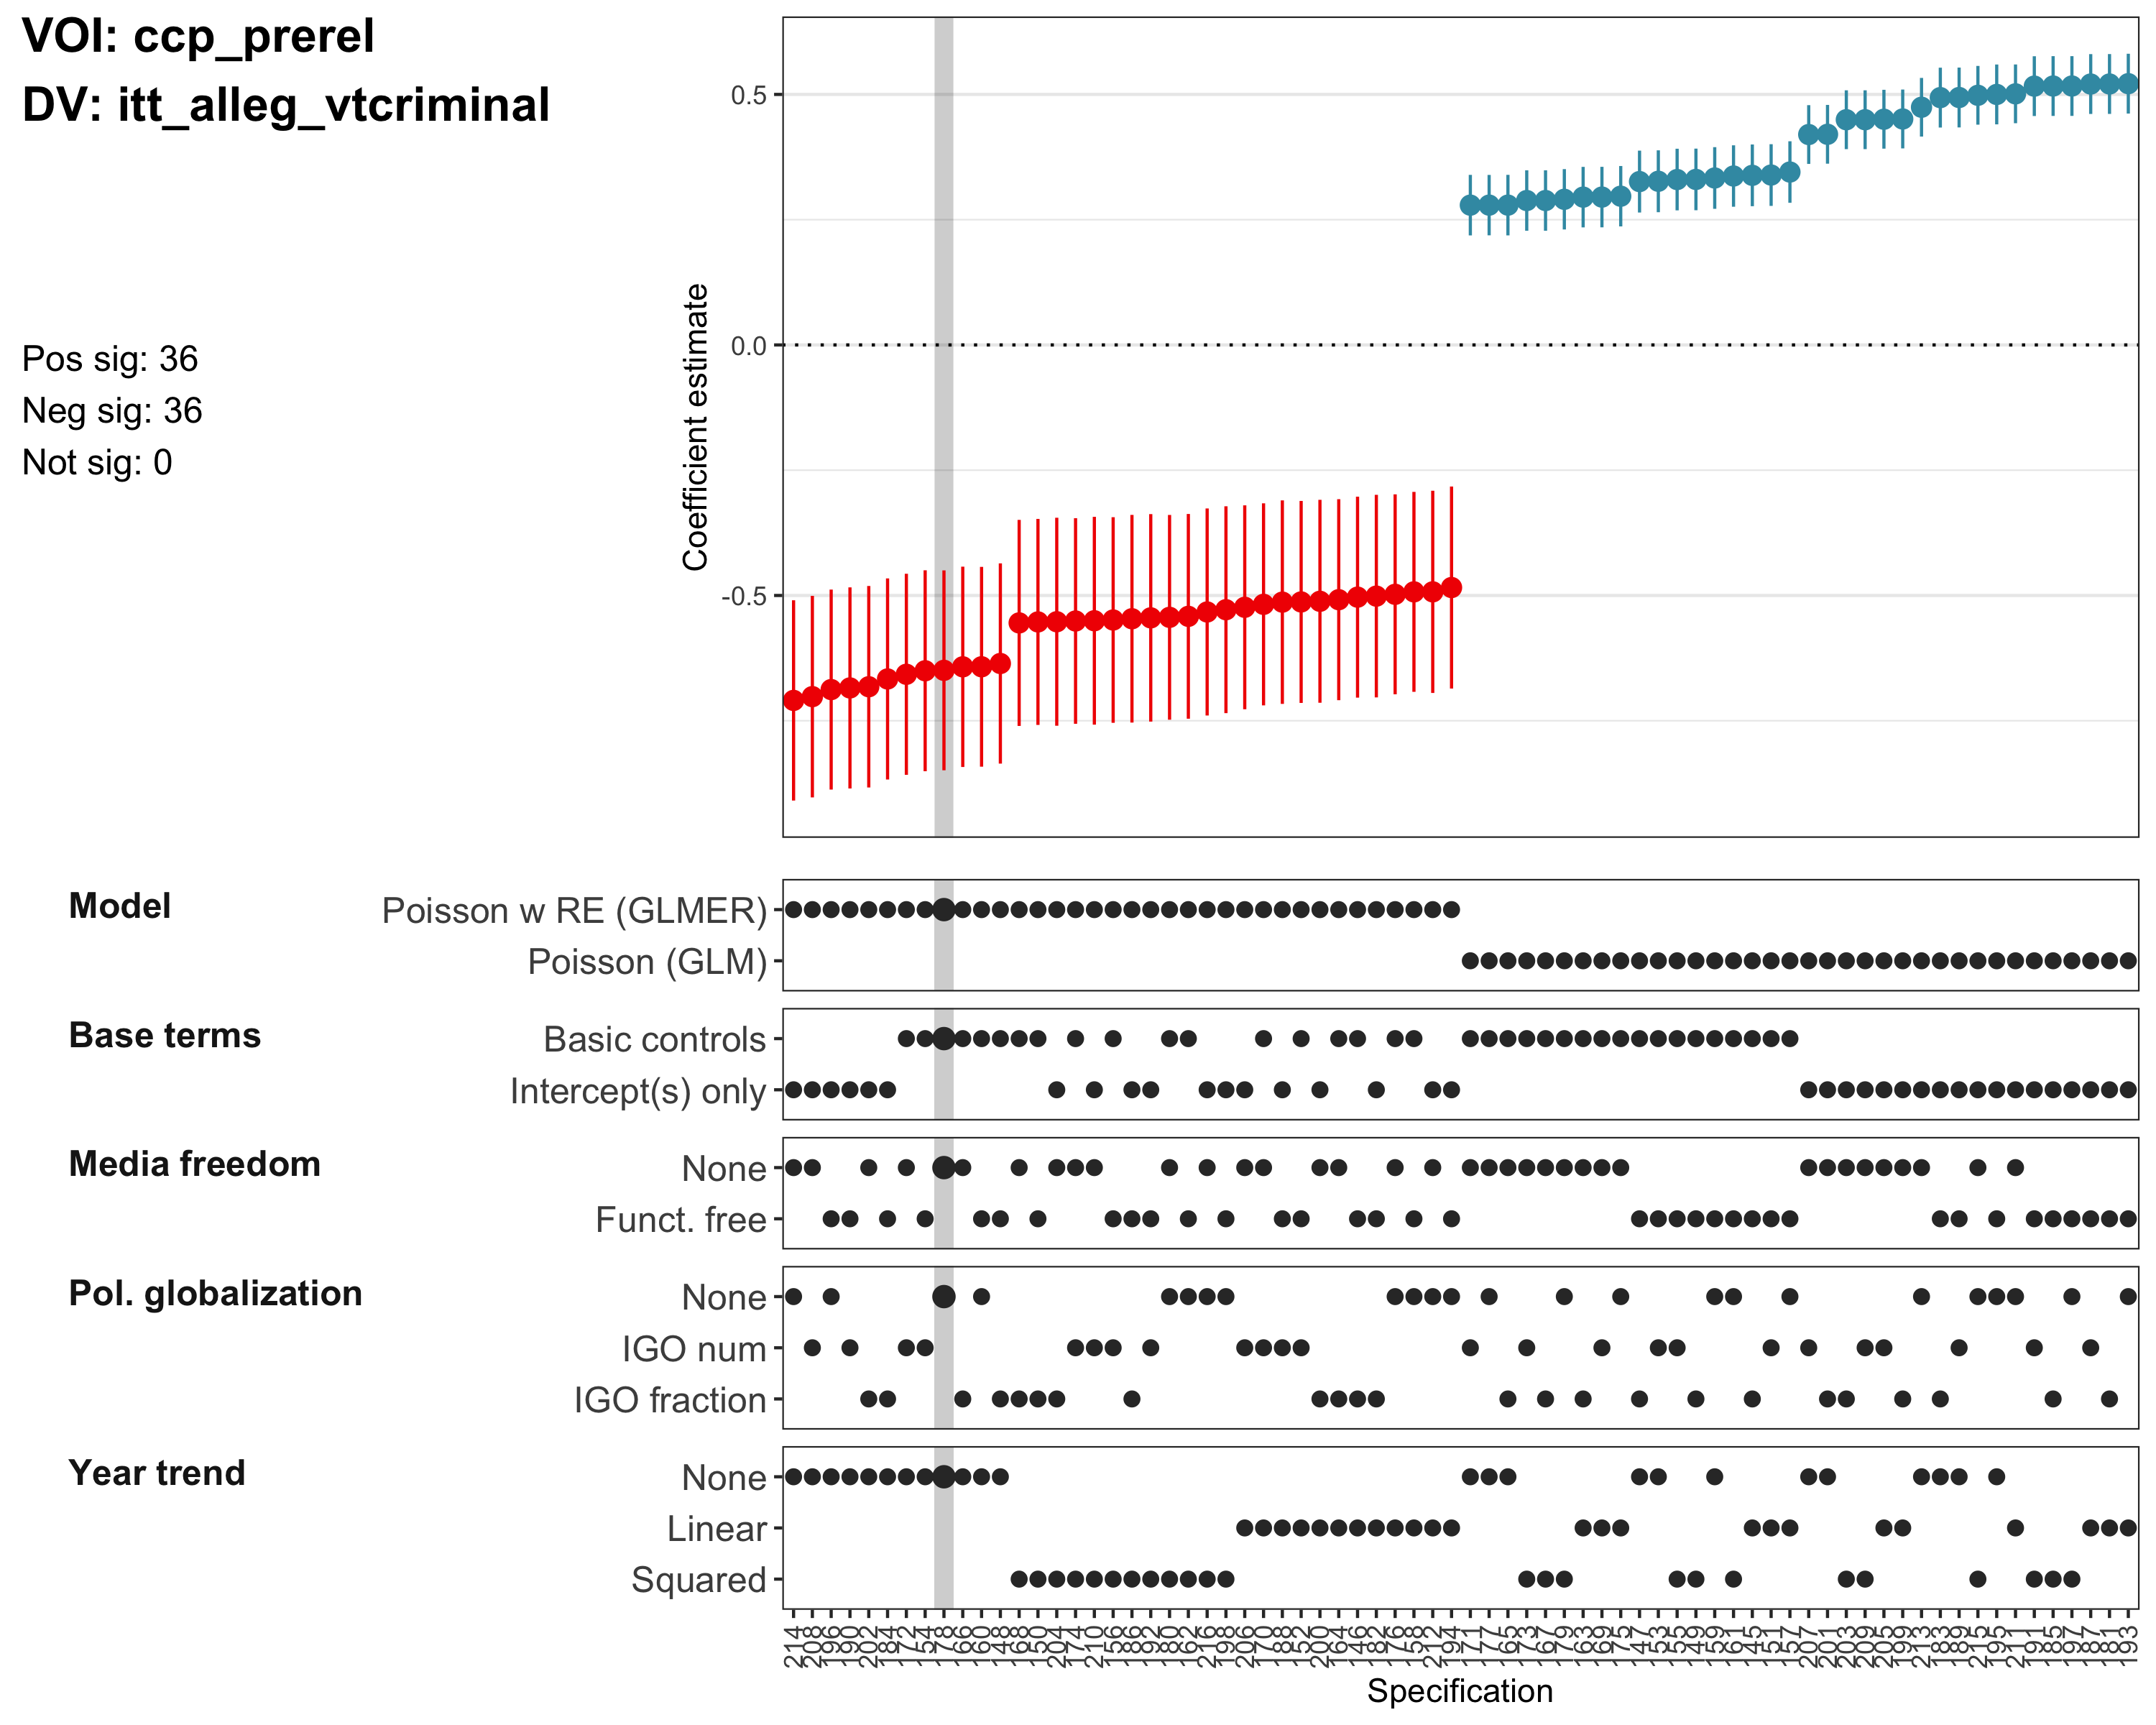
\includegraphics[height=4in]{../output/figures-robustness/specplot-ccp_prerel-itt_alleg_vtcriminal.png}

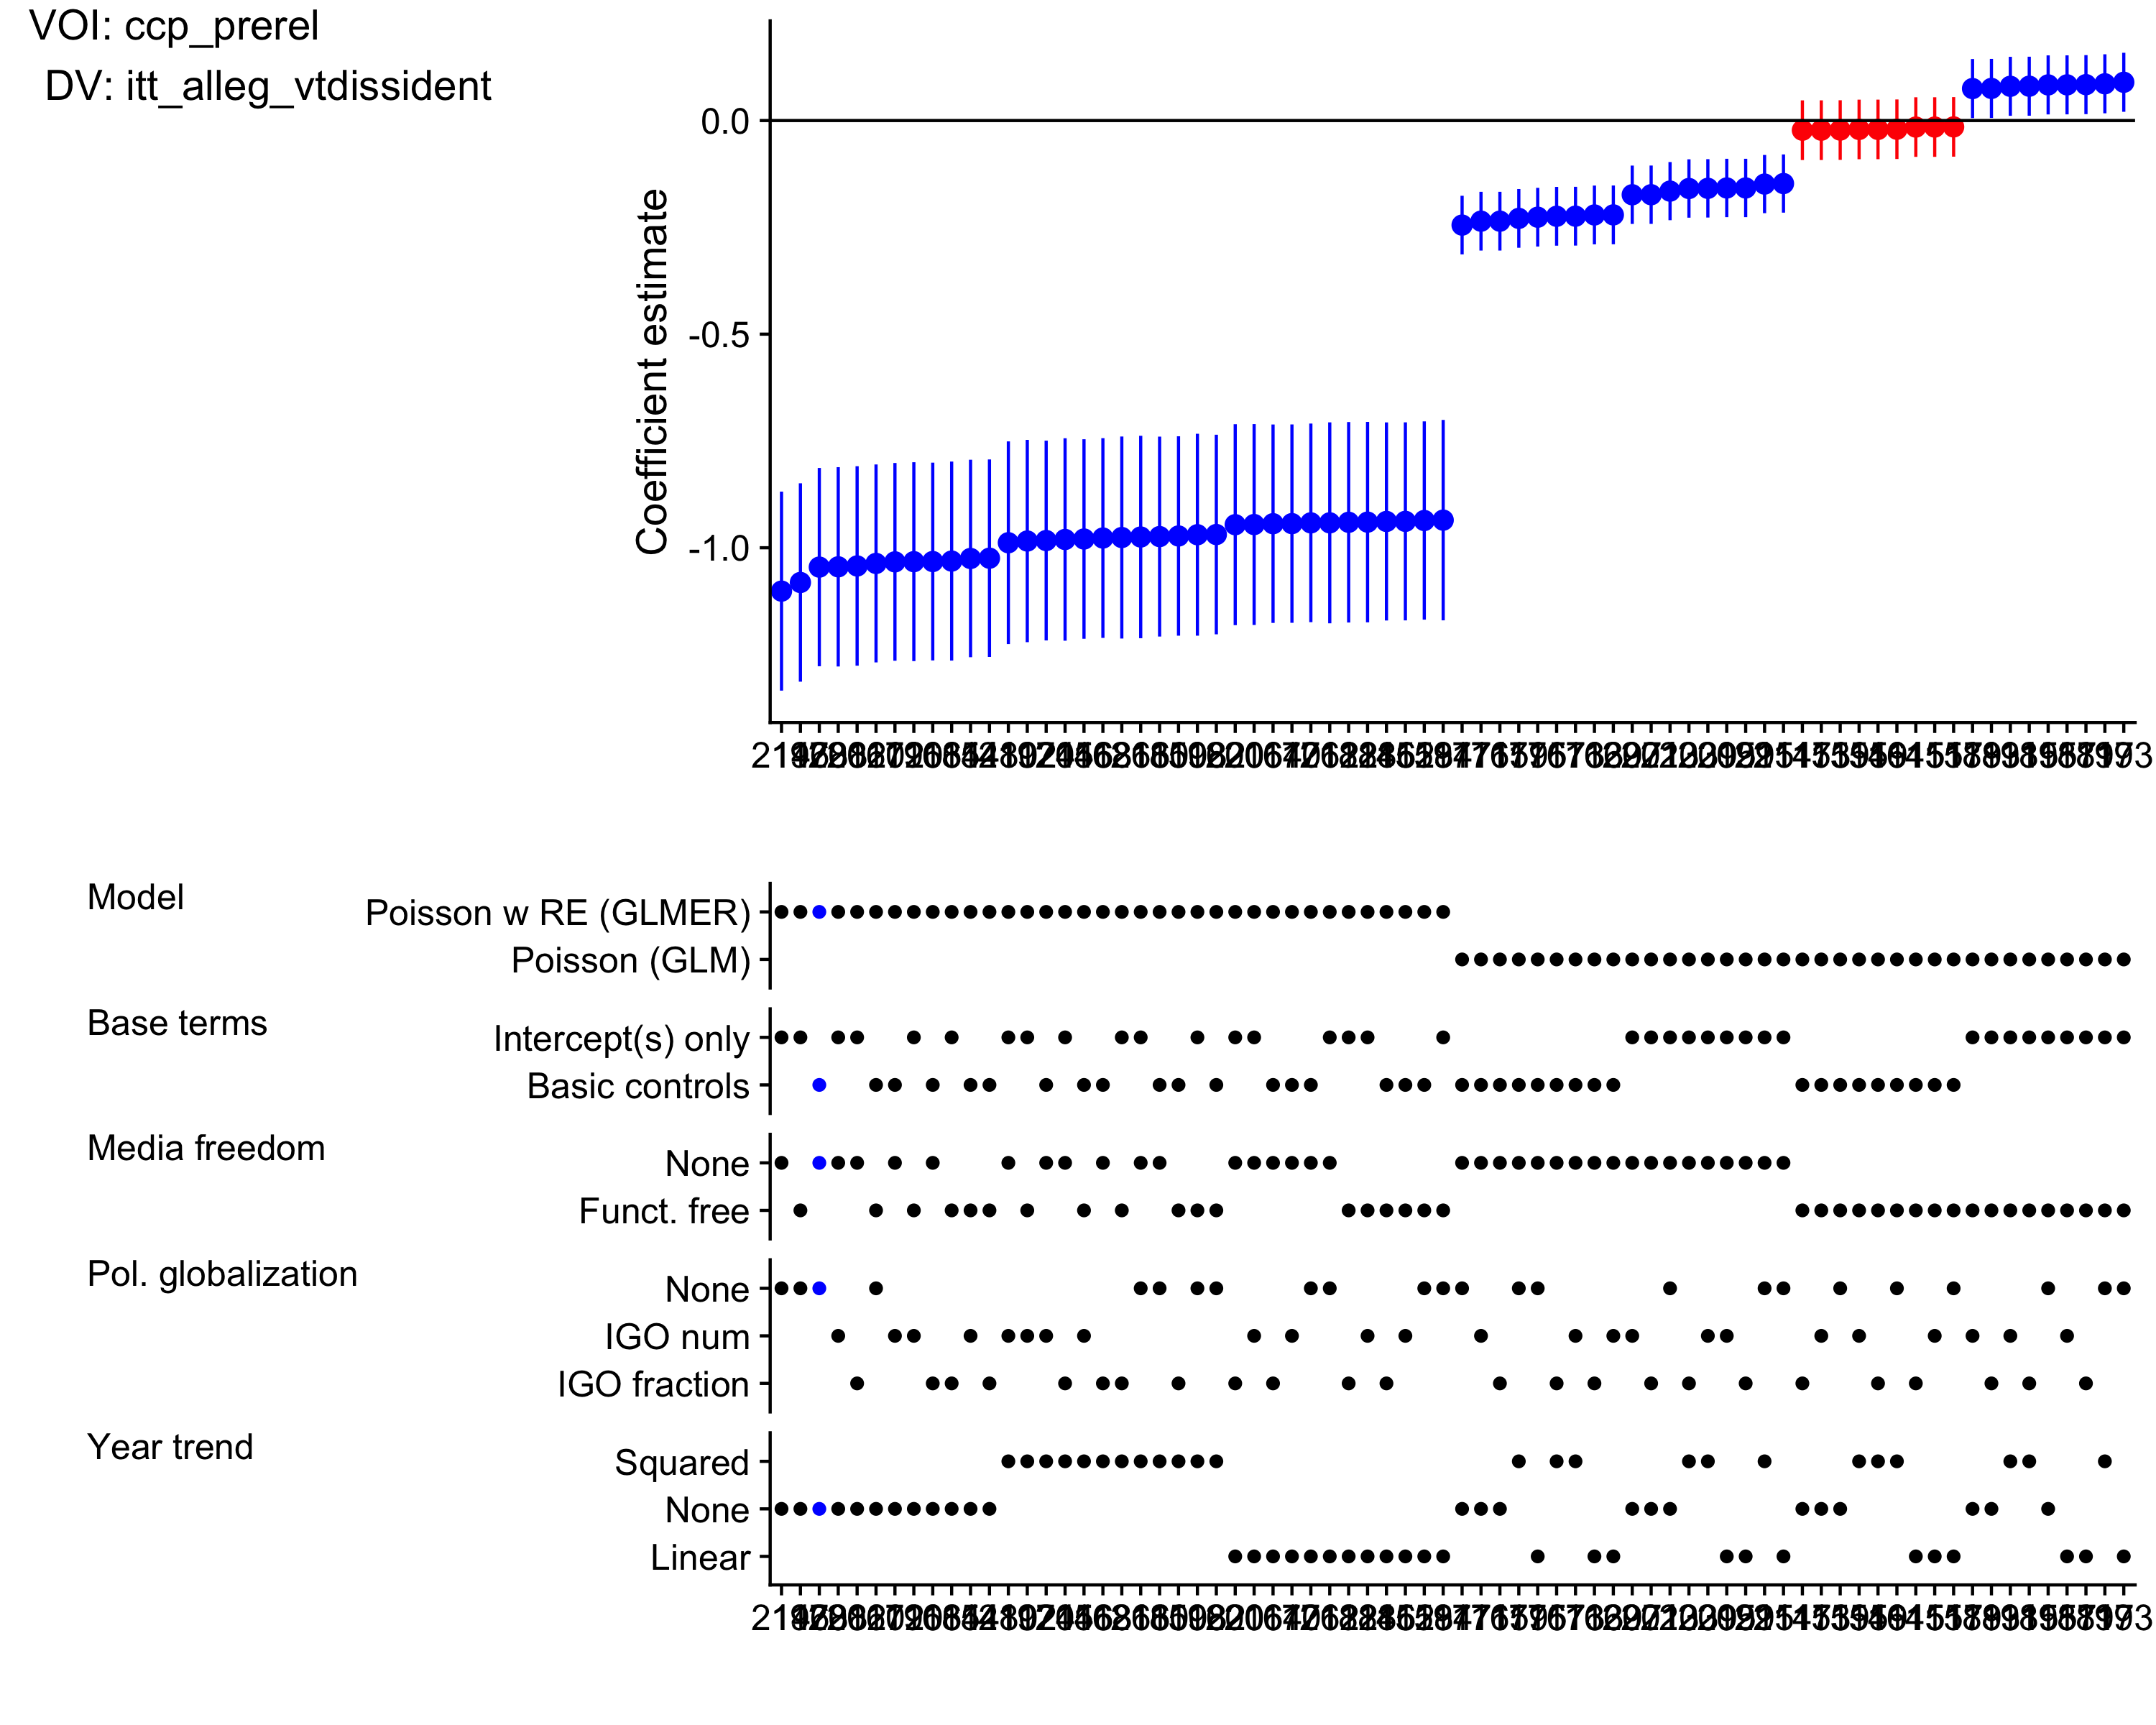
\includegraphics[height=4in]{../output/figures-robustness/specplot-ccp_prerel-itt_alleg_vtdissident.png}

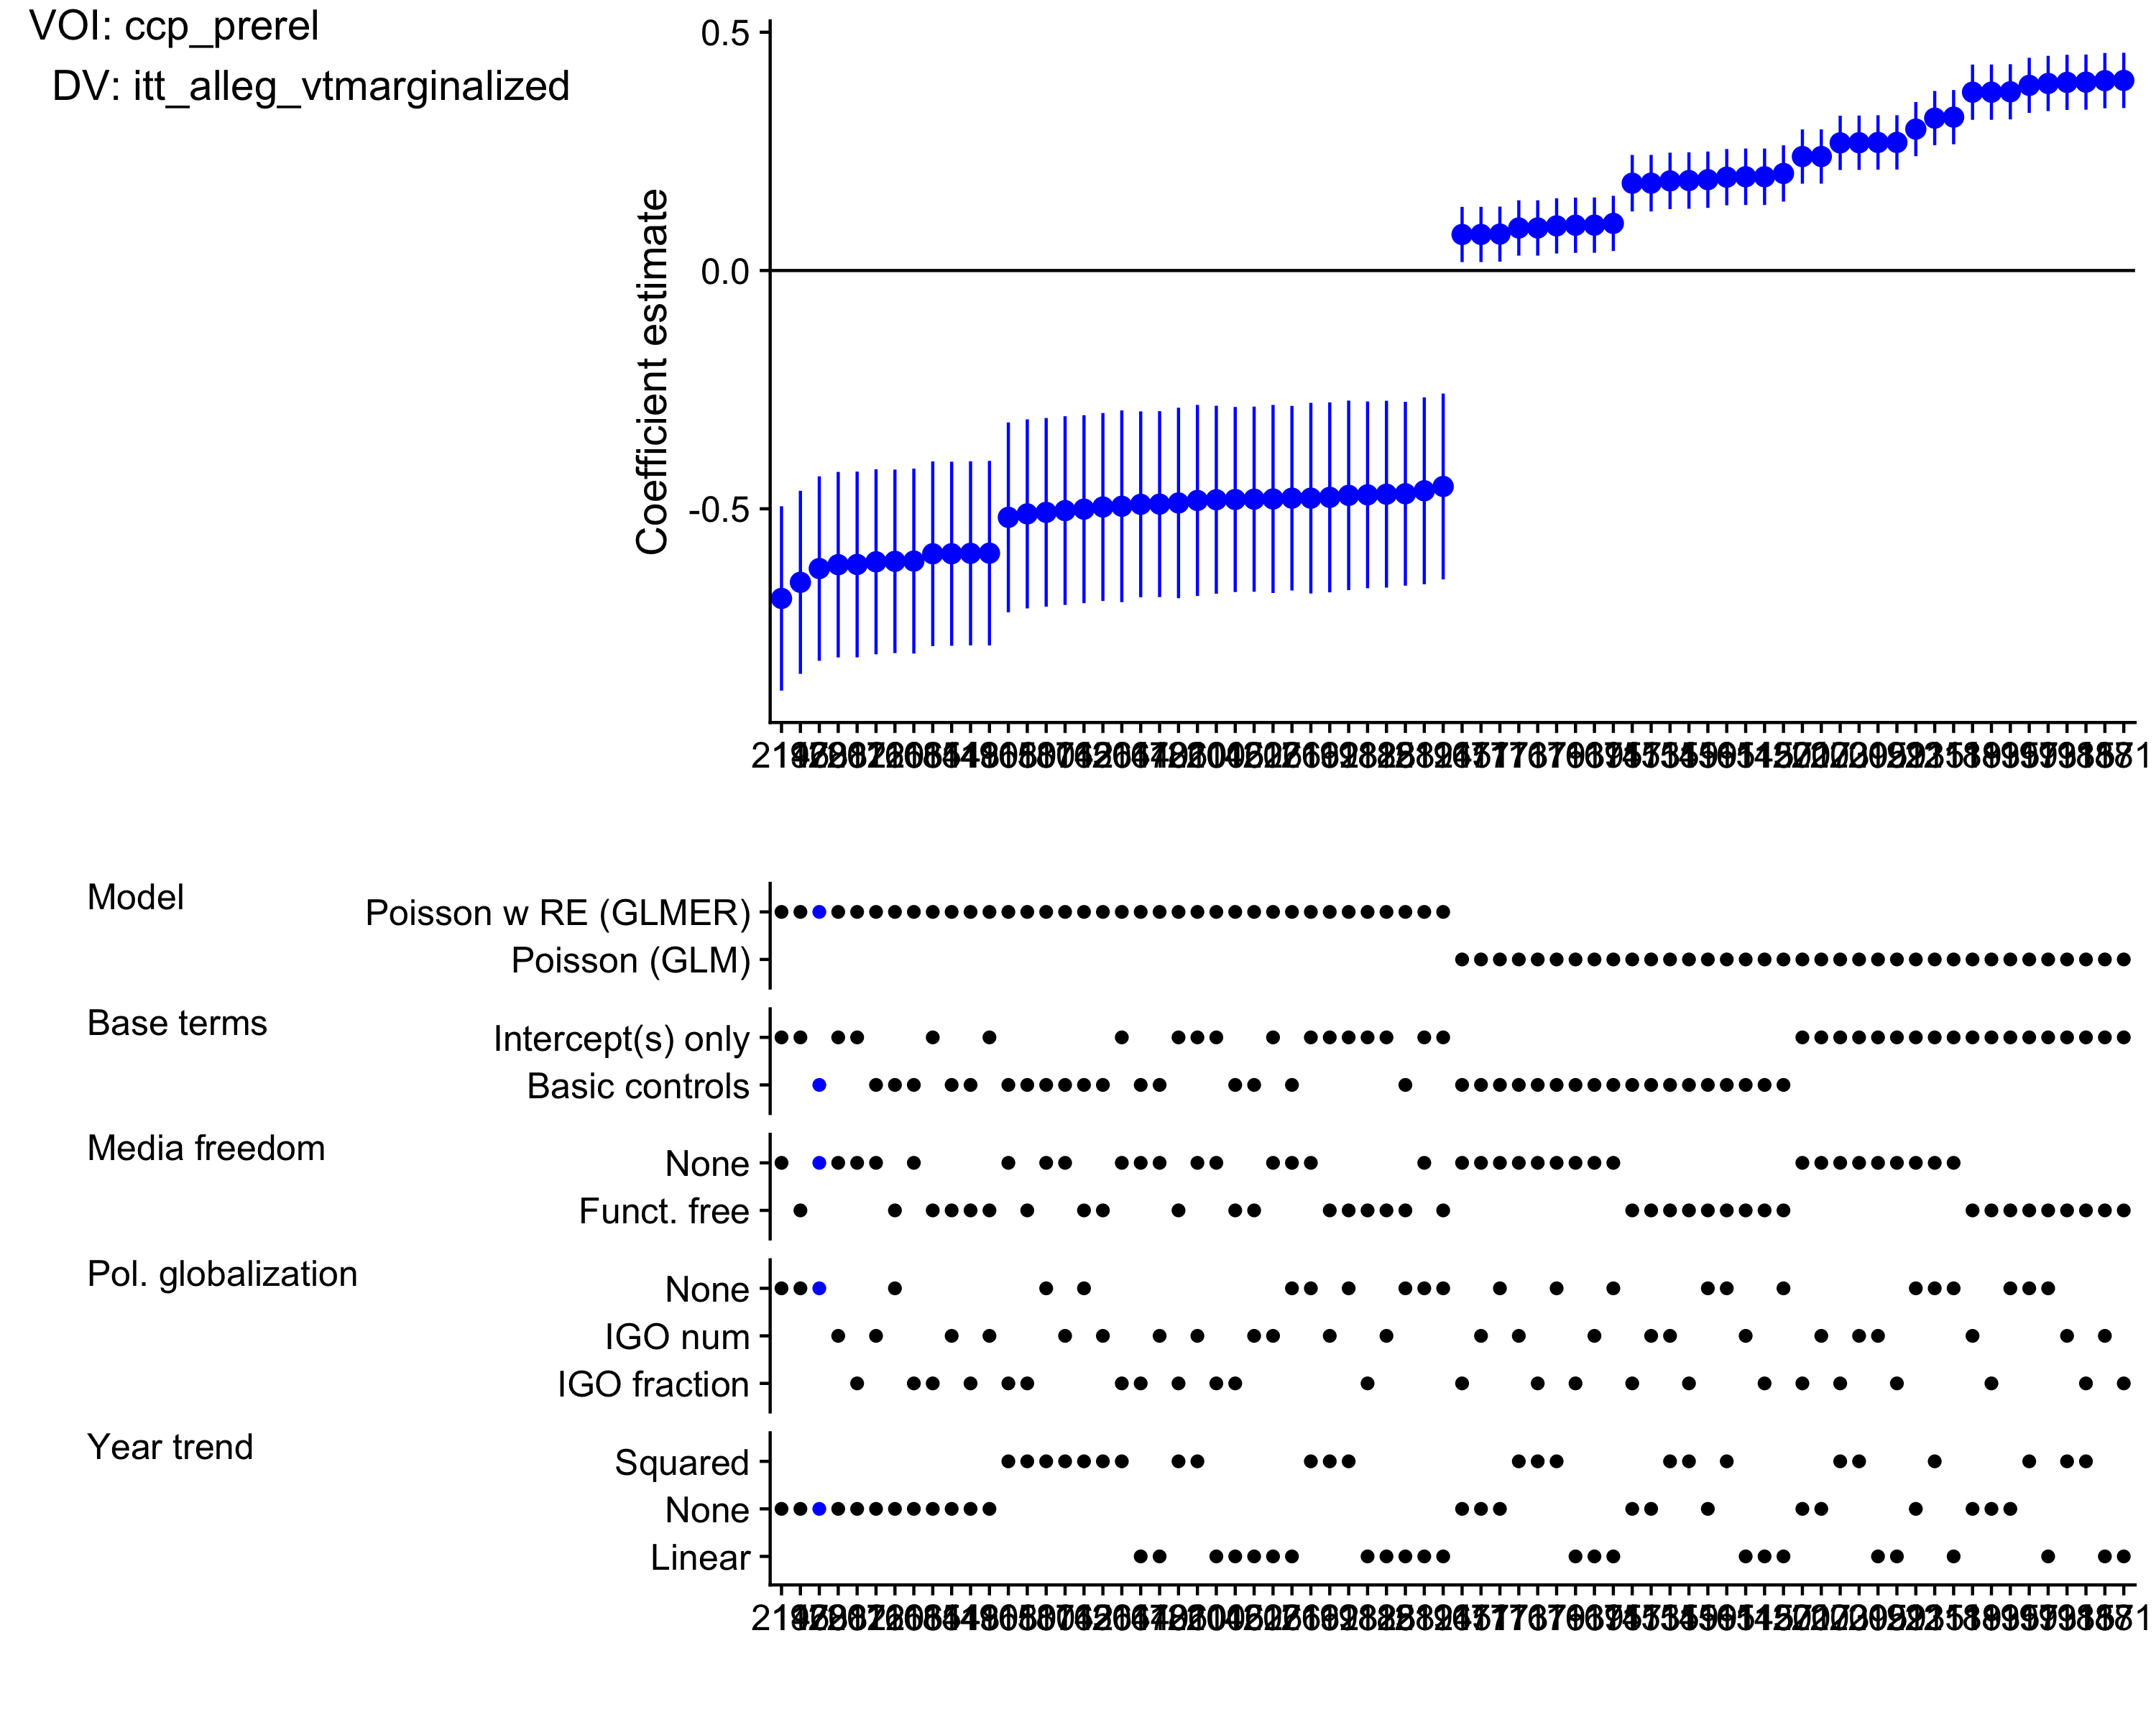
\includegraphics[height=4in]{../output/figures-robustness/specplot-ccp_prerel-itt_alleg_vtmarginalized.png}

\hypertarget{voi-ccp_speedtri}{%
\subsection{VOI: ccp\_speedtri}\label{voi-ccp_speedtri}}

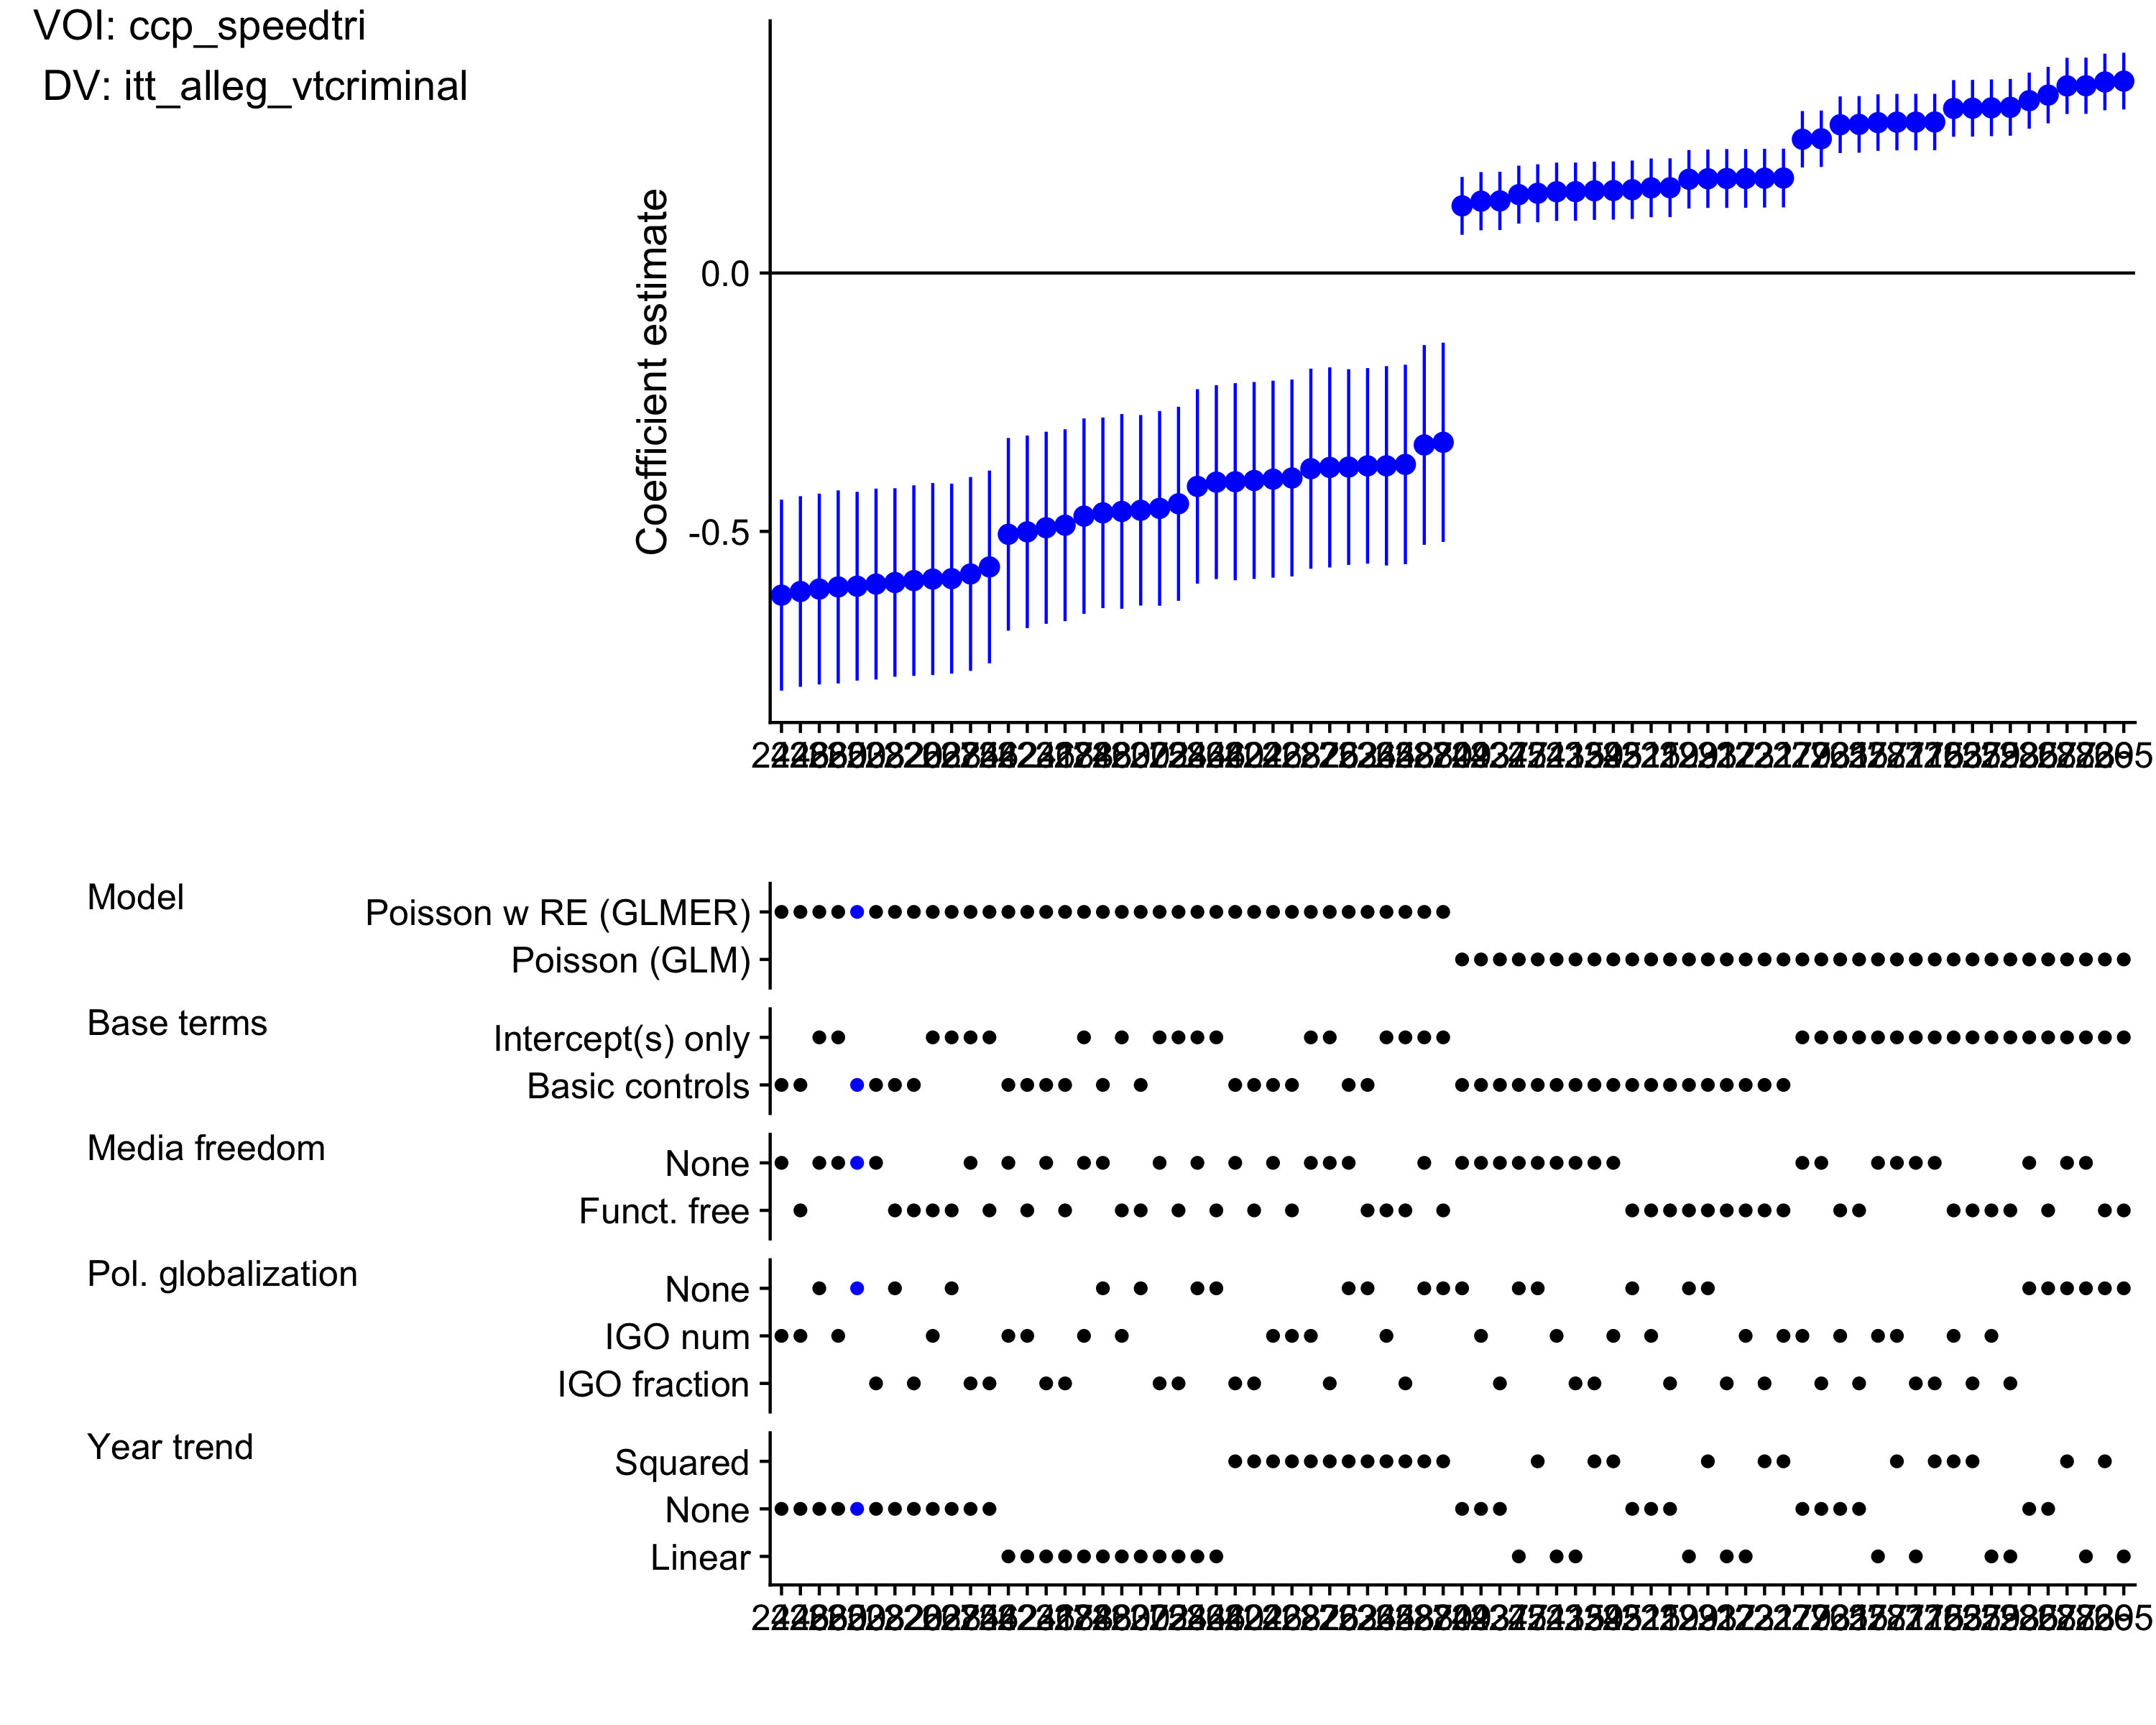
\includegraphics[height=4in]{../output/figures-robustness/specplot-ccp_speedtri-itt_alleg_vtcriminal.png}

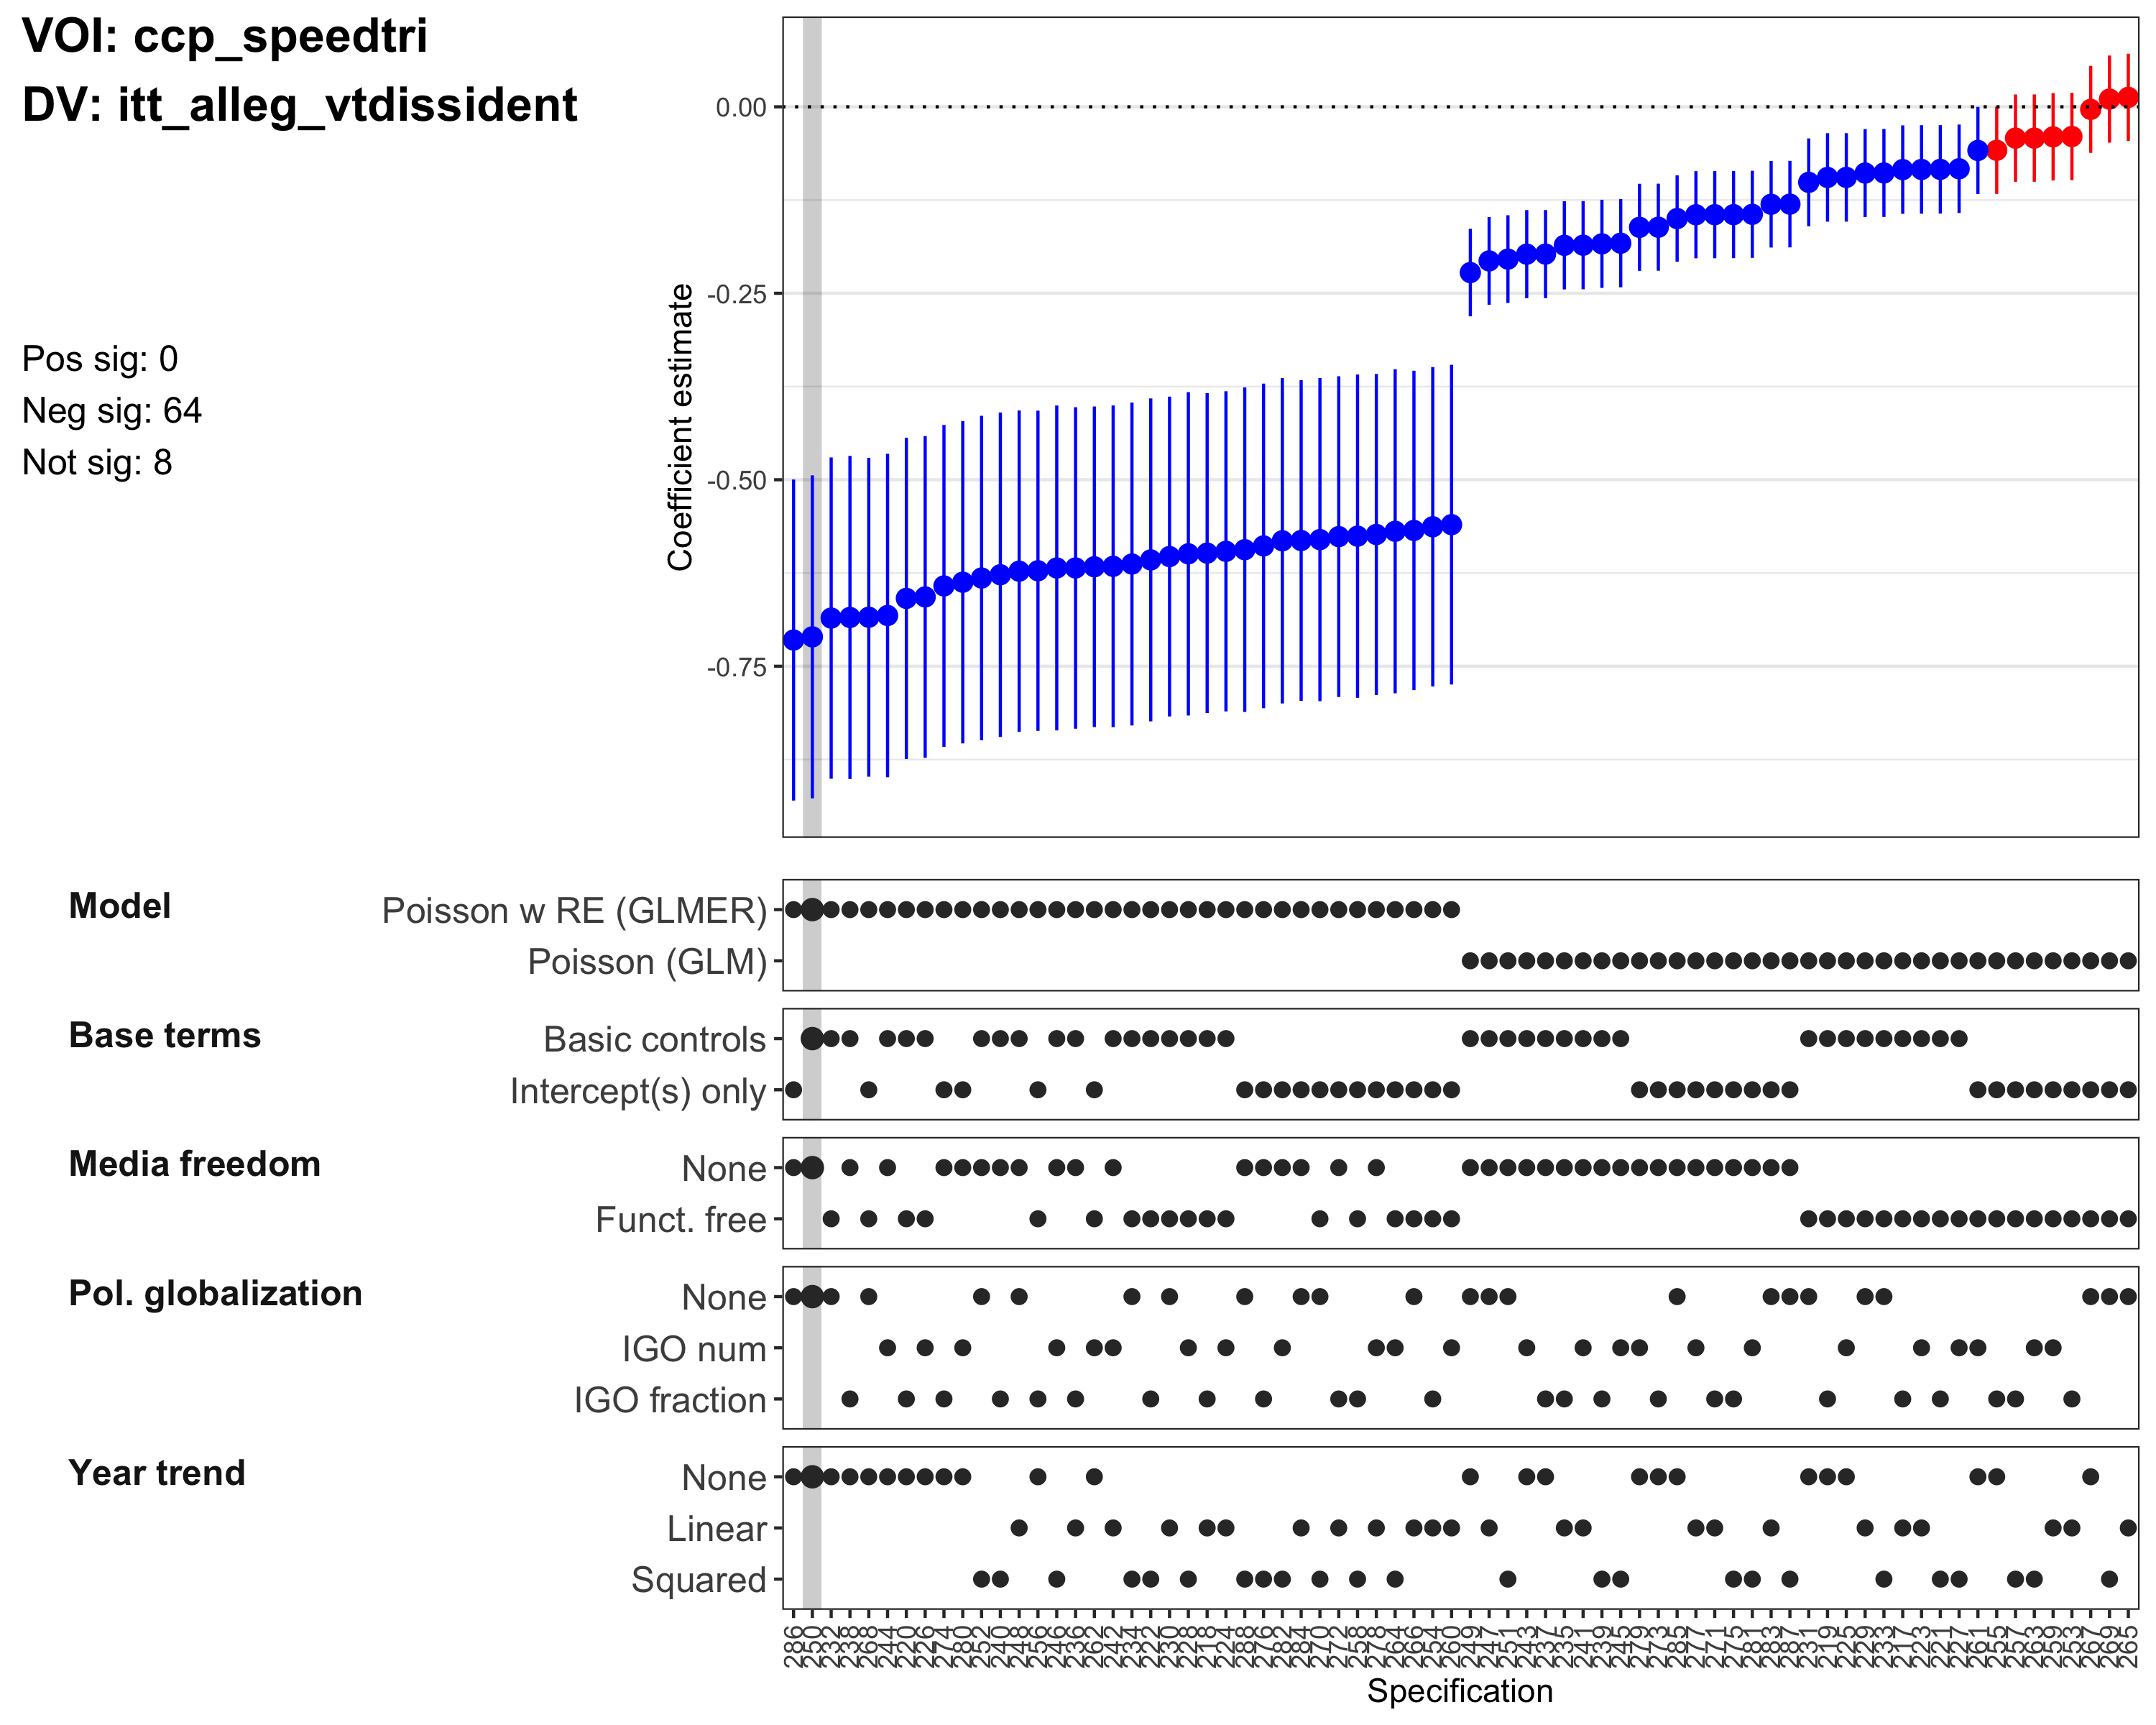
\includegraphics[height=4in]{../output/figures-robustness/specplot-ccp_speedtri-itt_alleg_vtdissident.png}

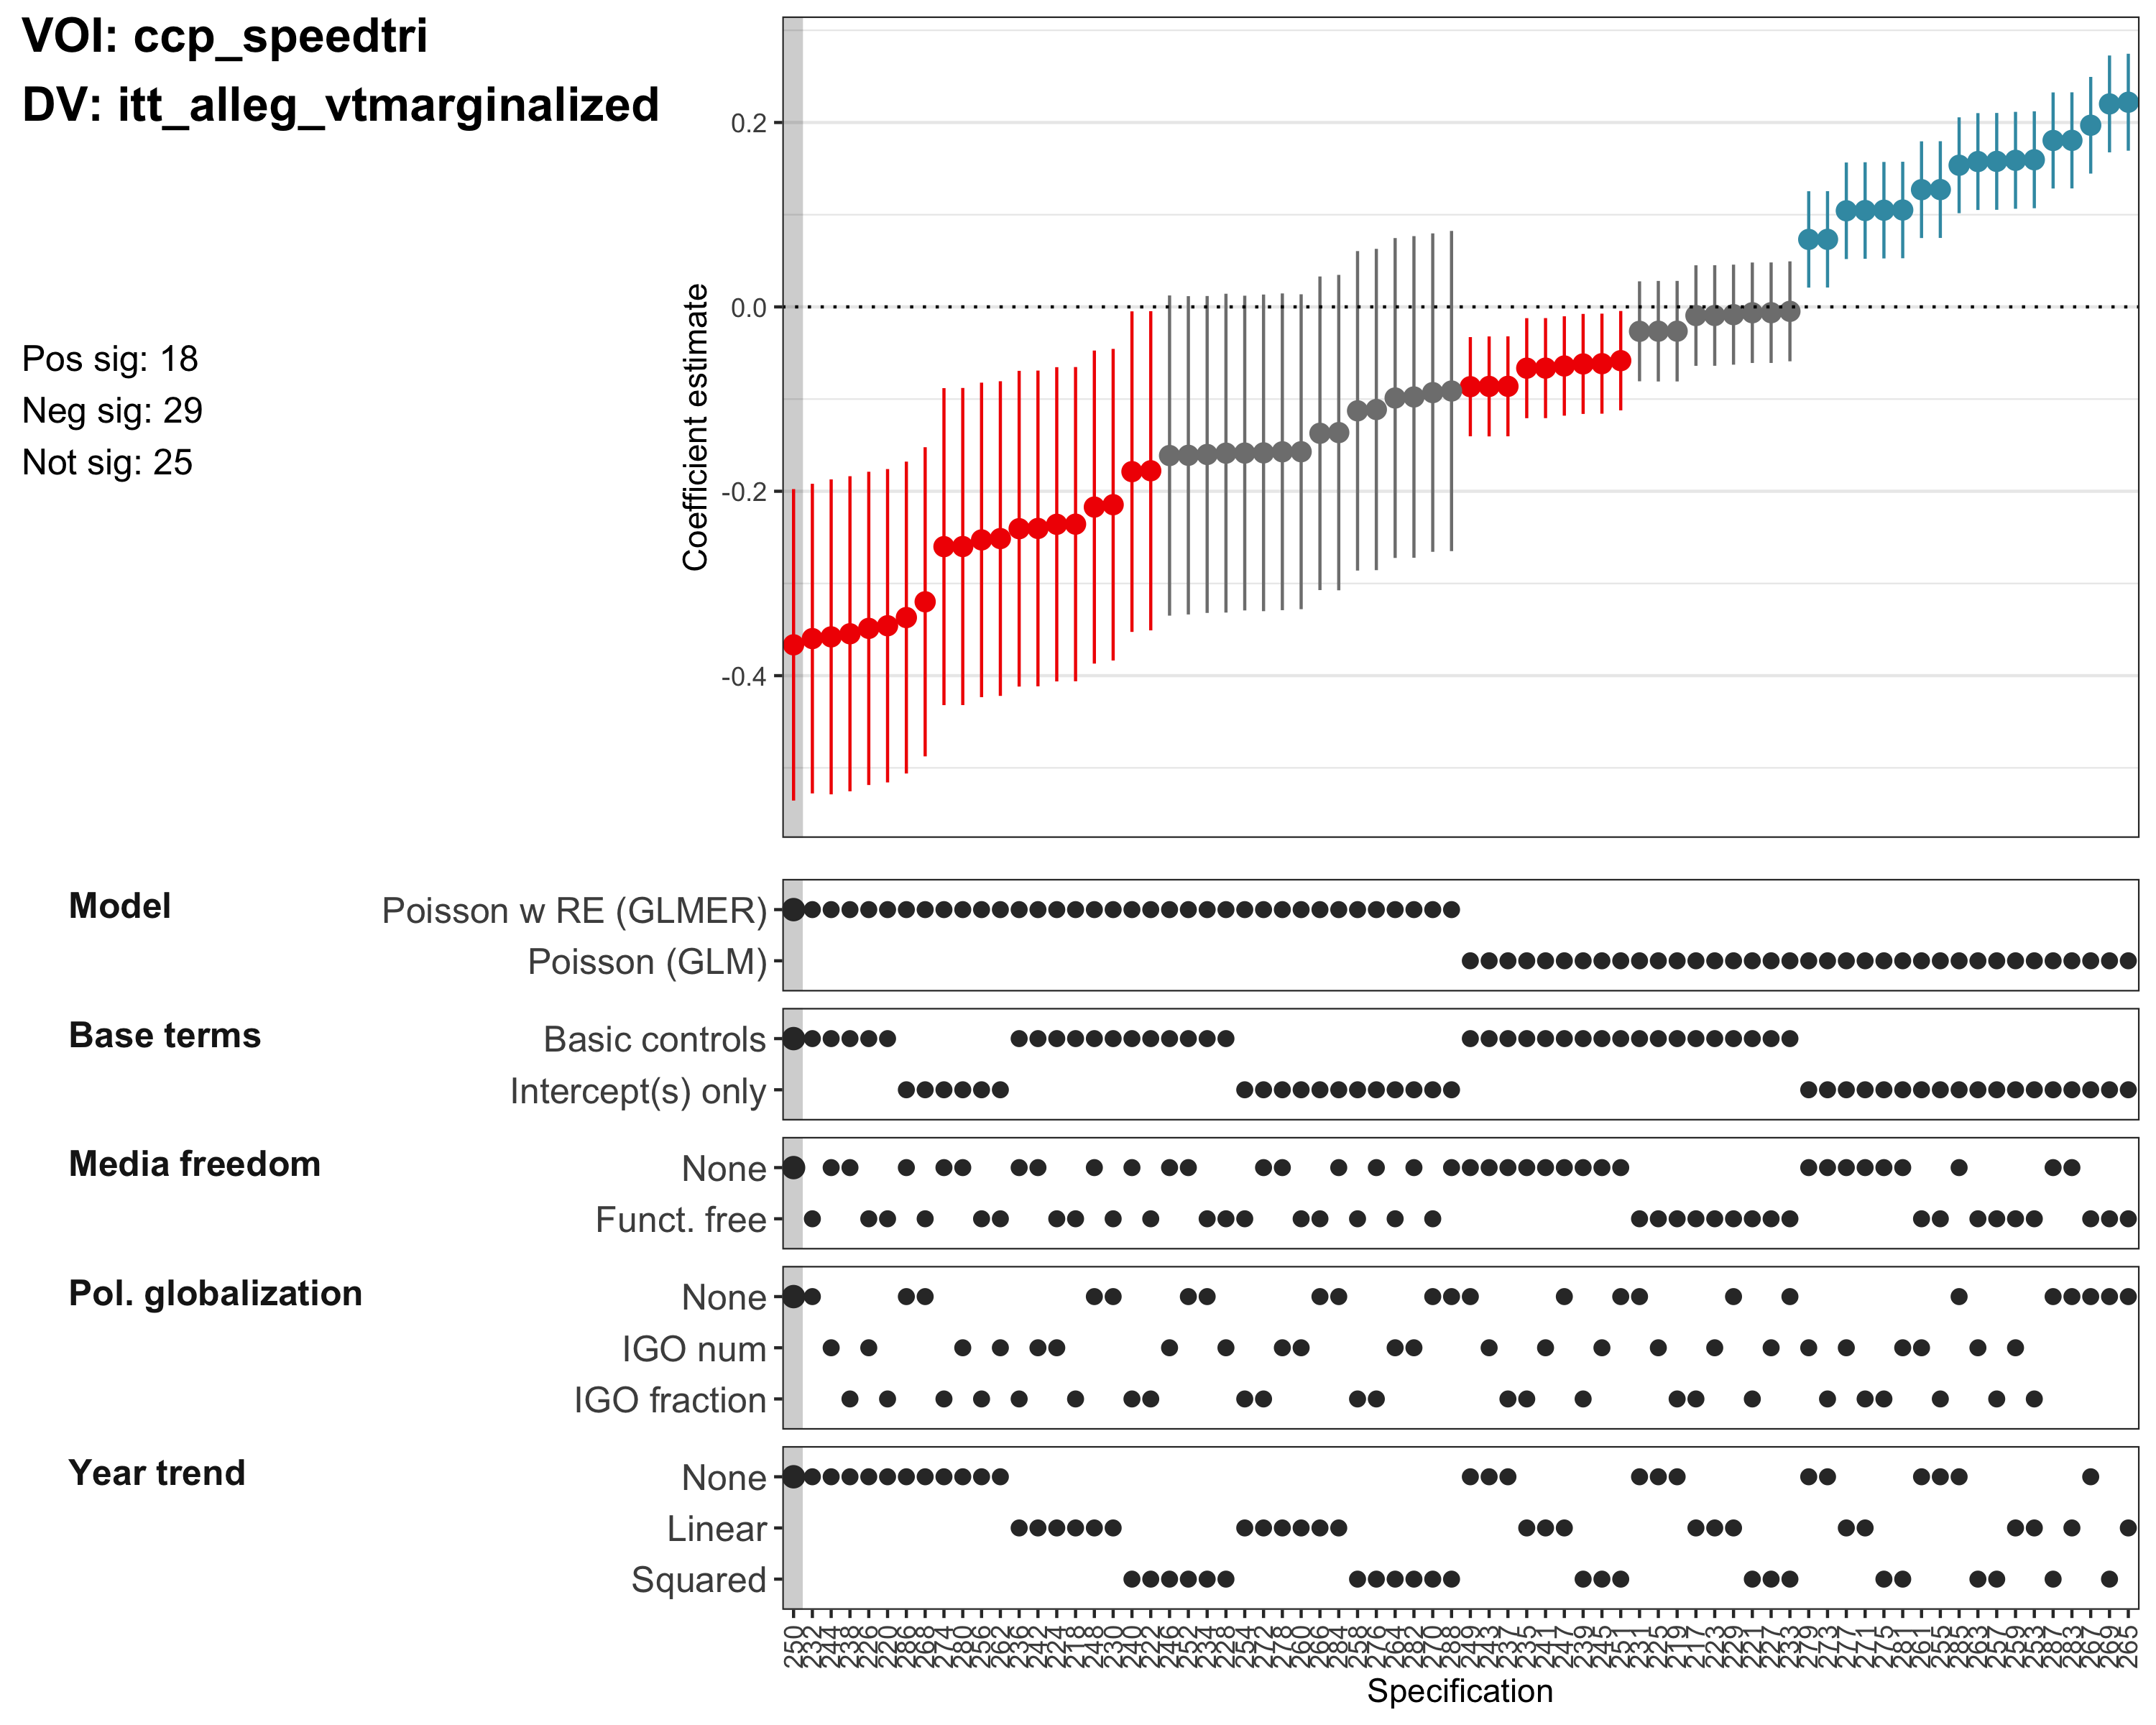
\includegraphics[height=4in]{../output/figures-robustness/specplot-ccp_speedtri-itt_alleg_vtmarginalized.png}

\hypertarget{voi-ccp_torture}{%
\subsection{VOI: ccp\_torture}\label{voi-ccp_torture}}

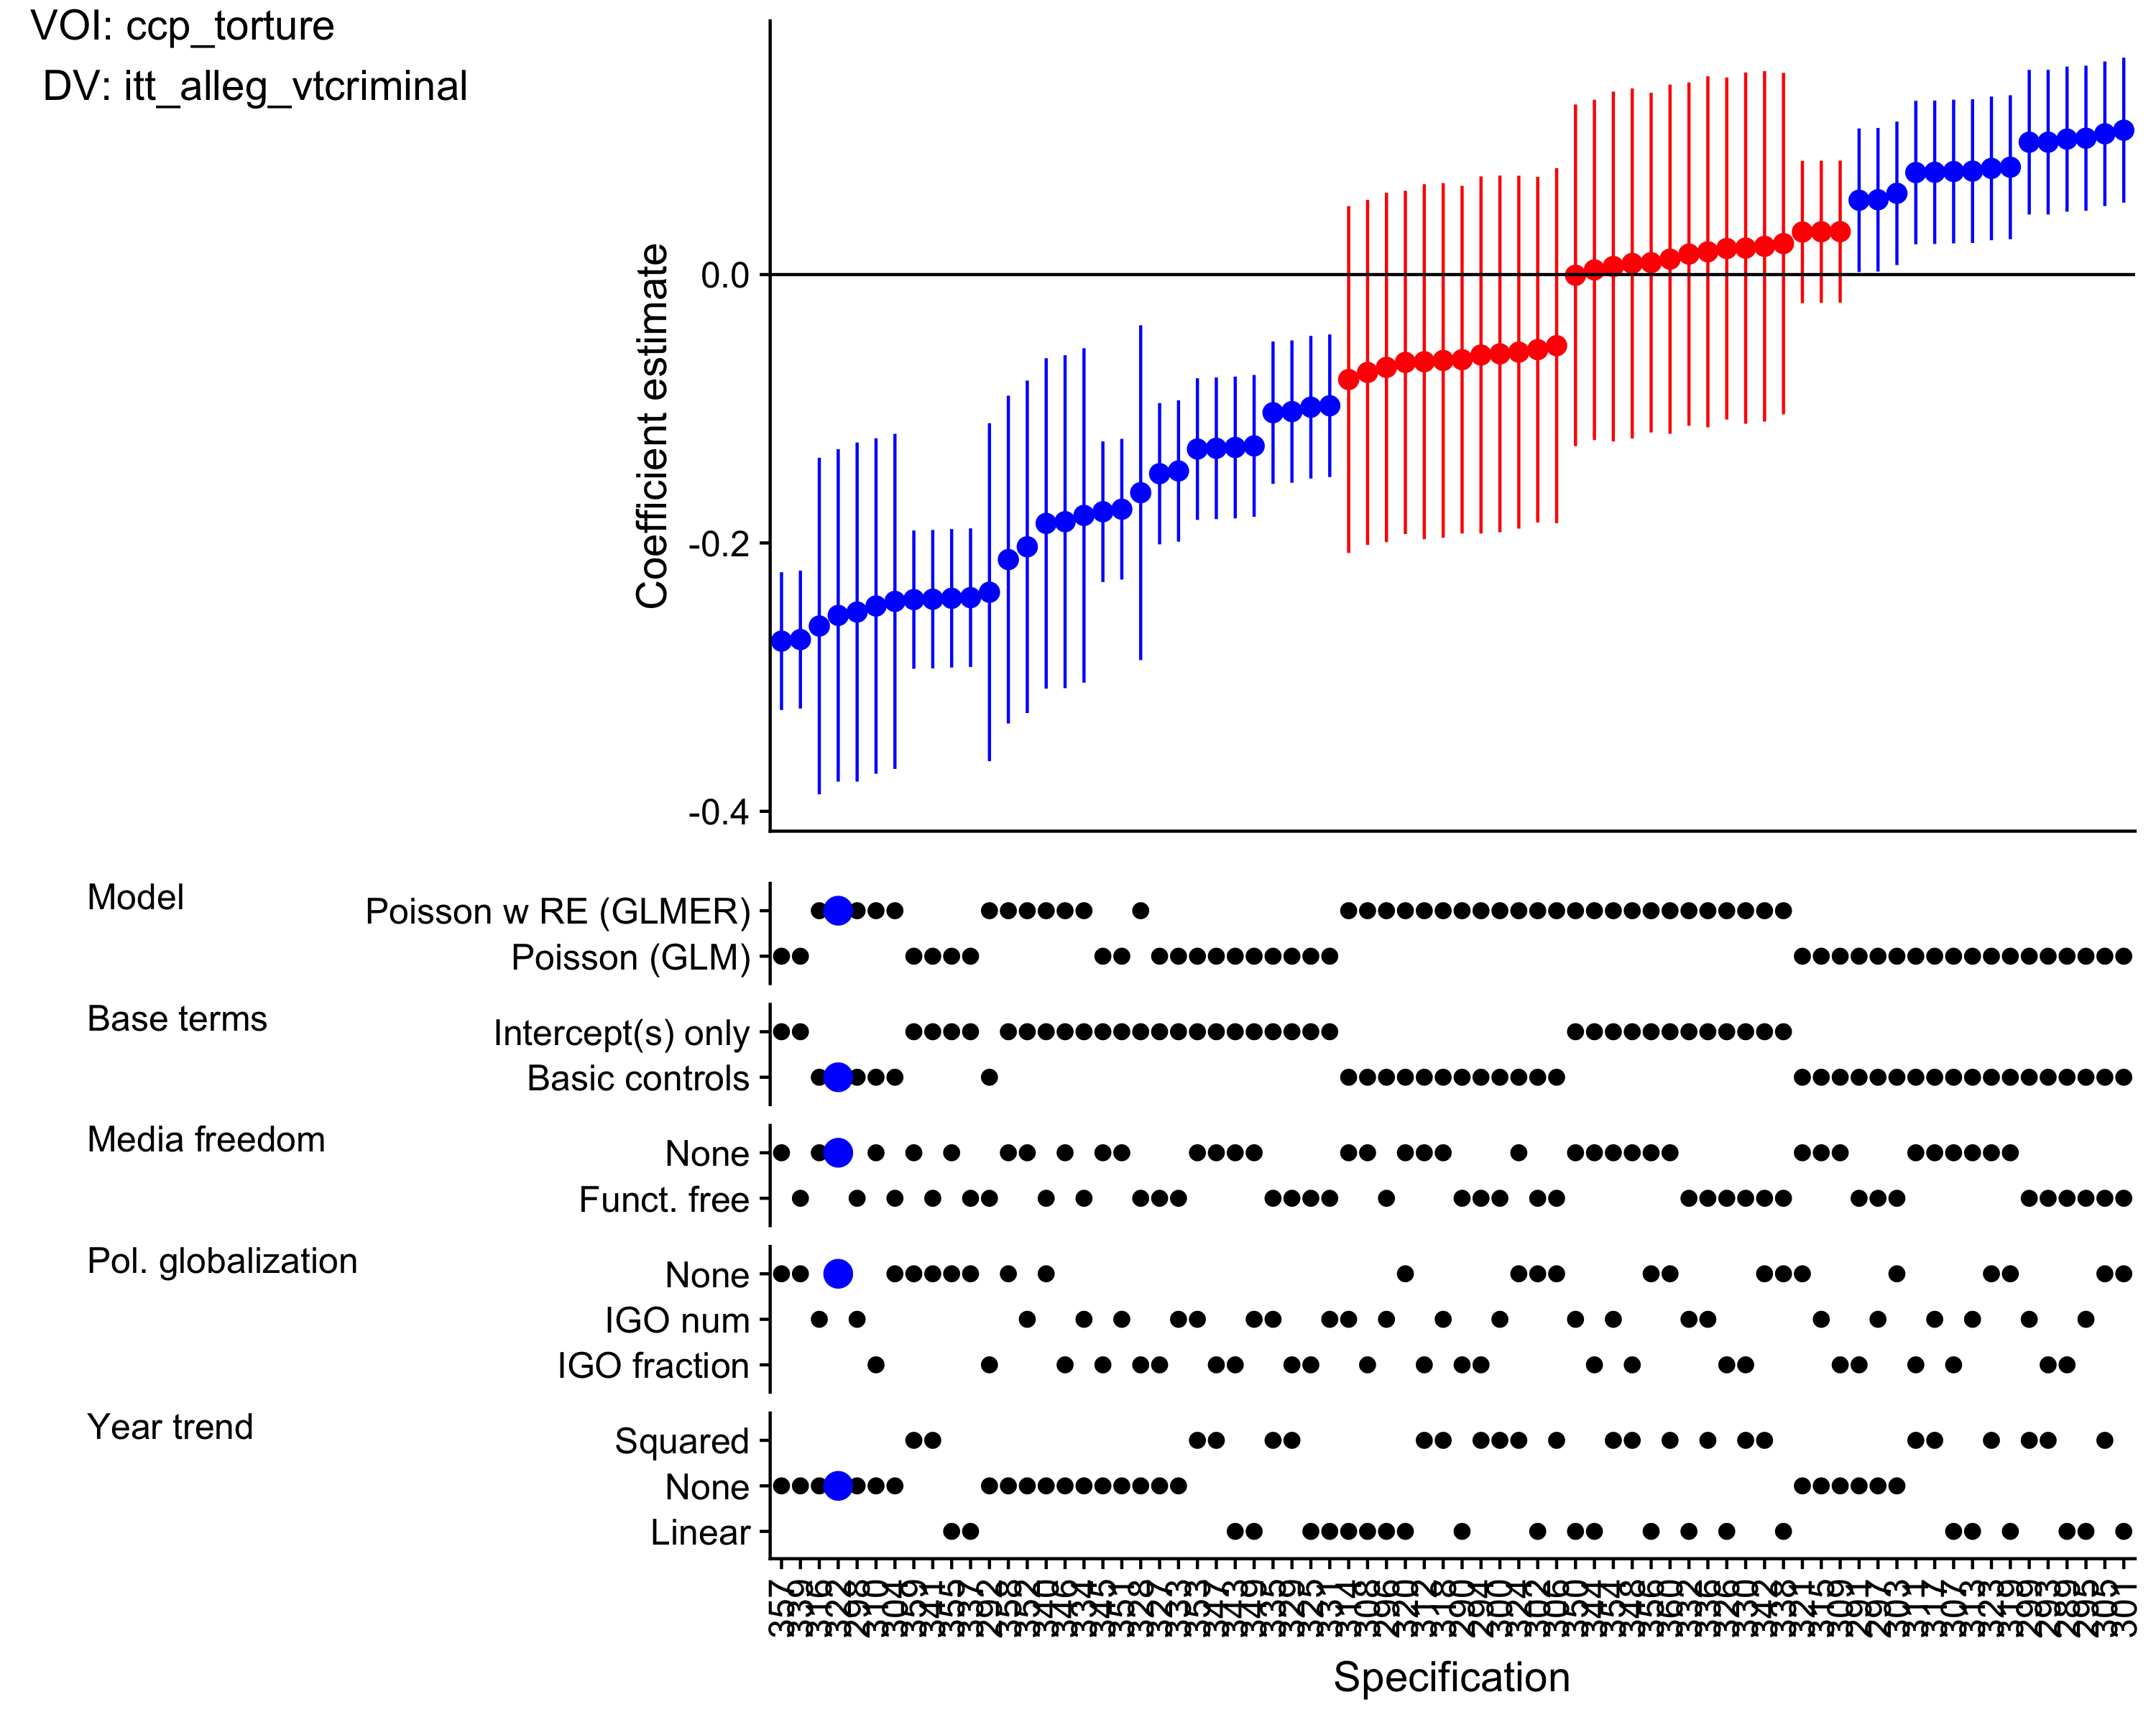
\includegraphics[height=4in]{../output/figures-robustness/specplot-ccp_torture-itt_alleg_vtcriminal.png}

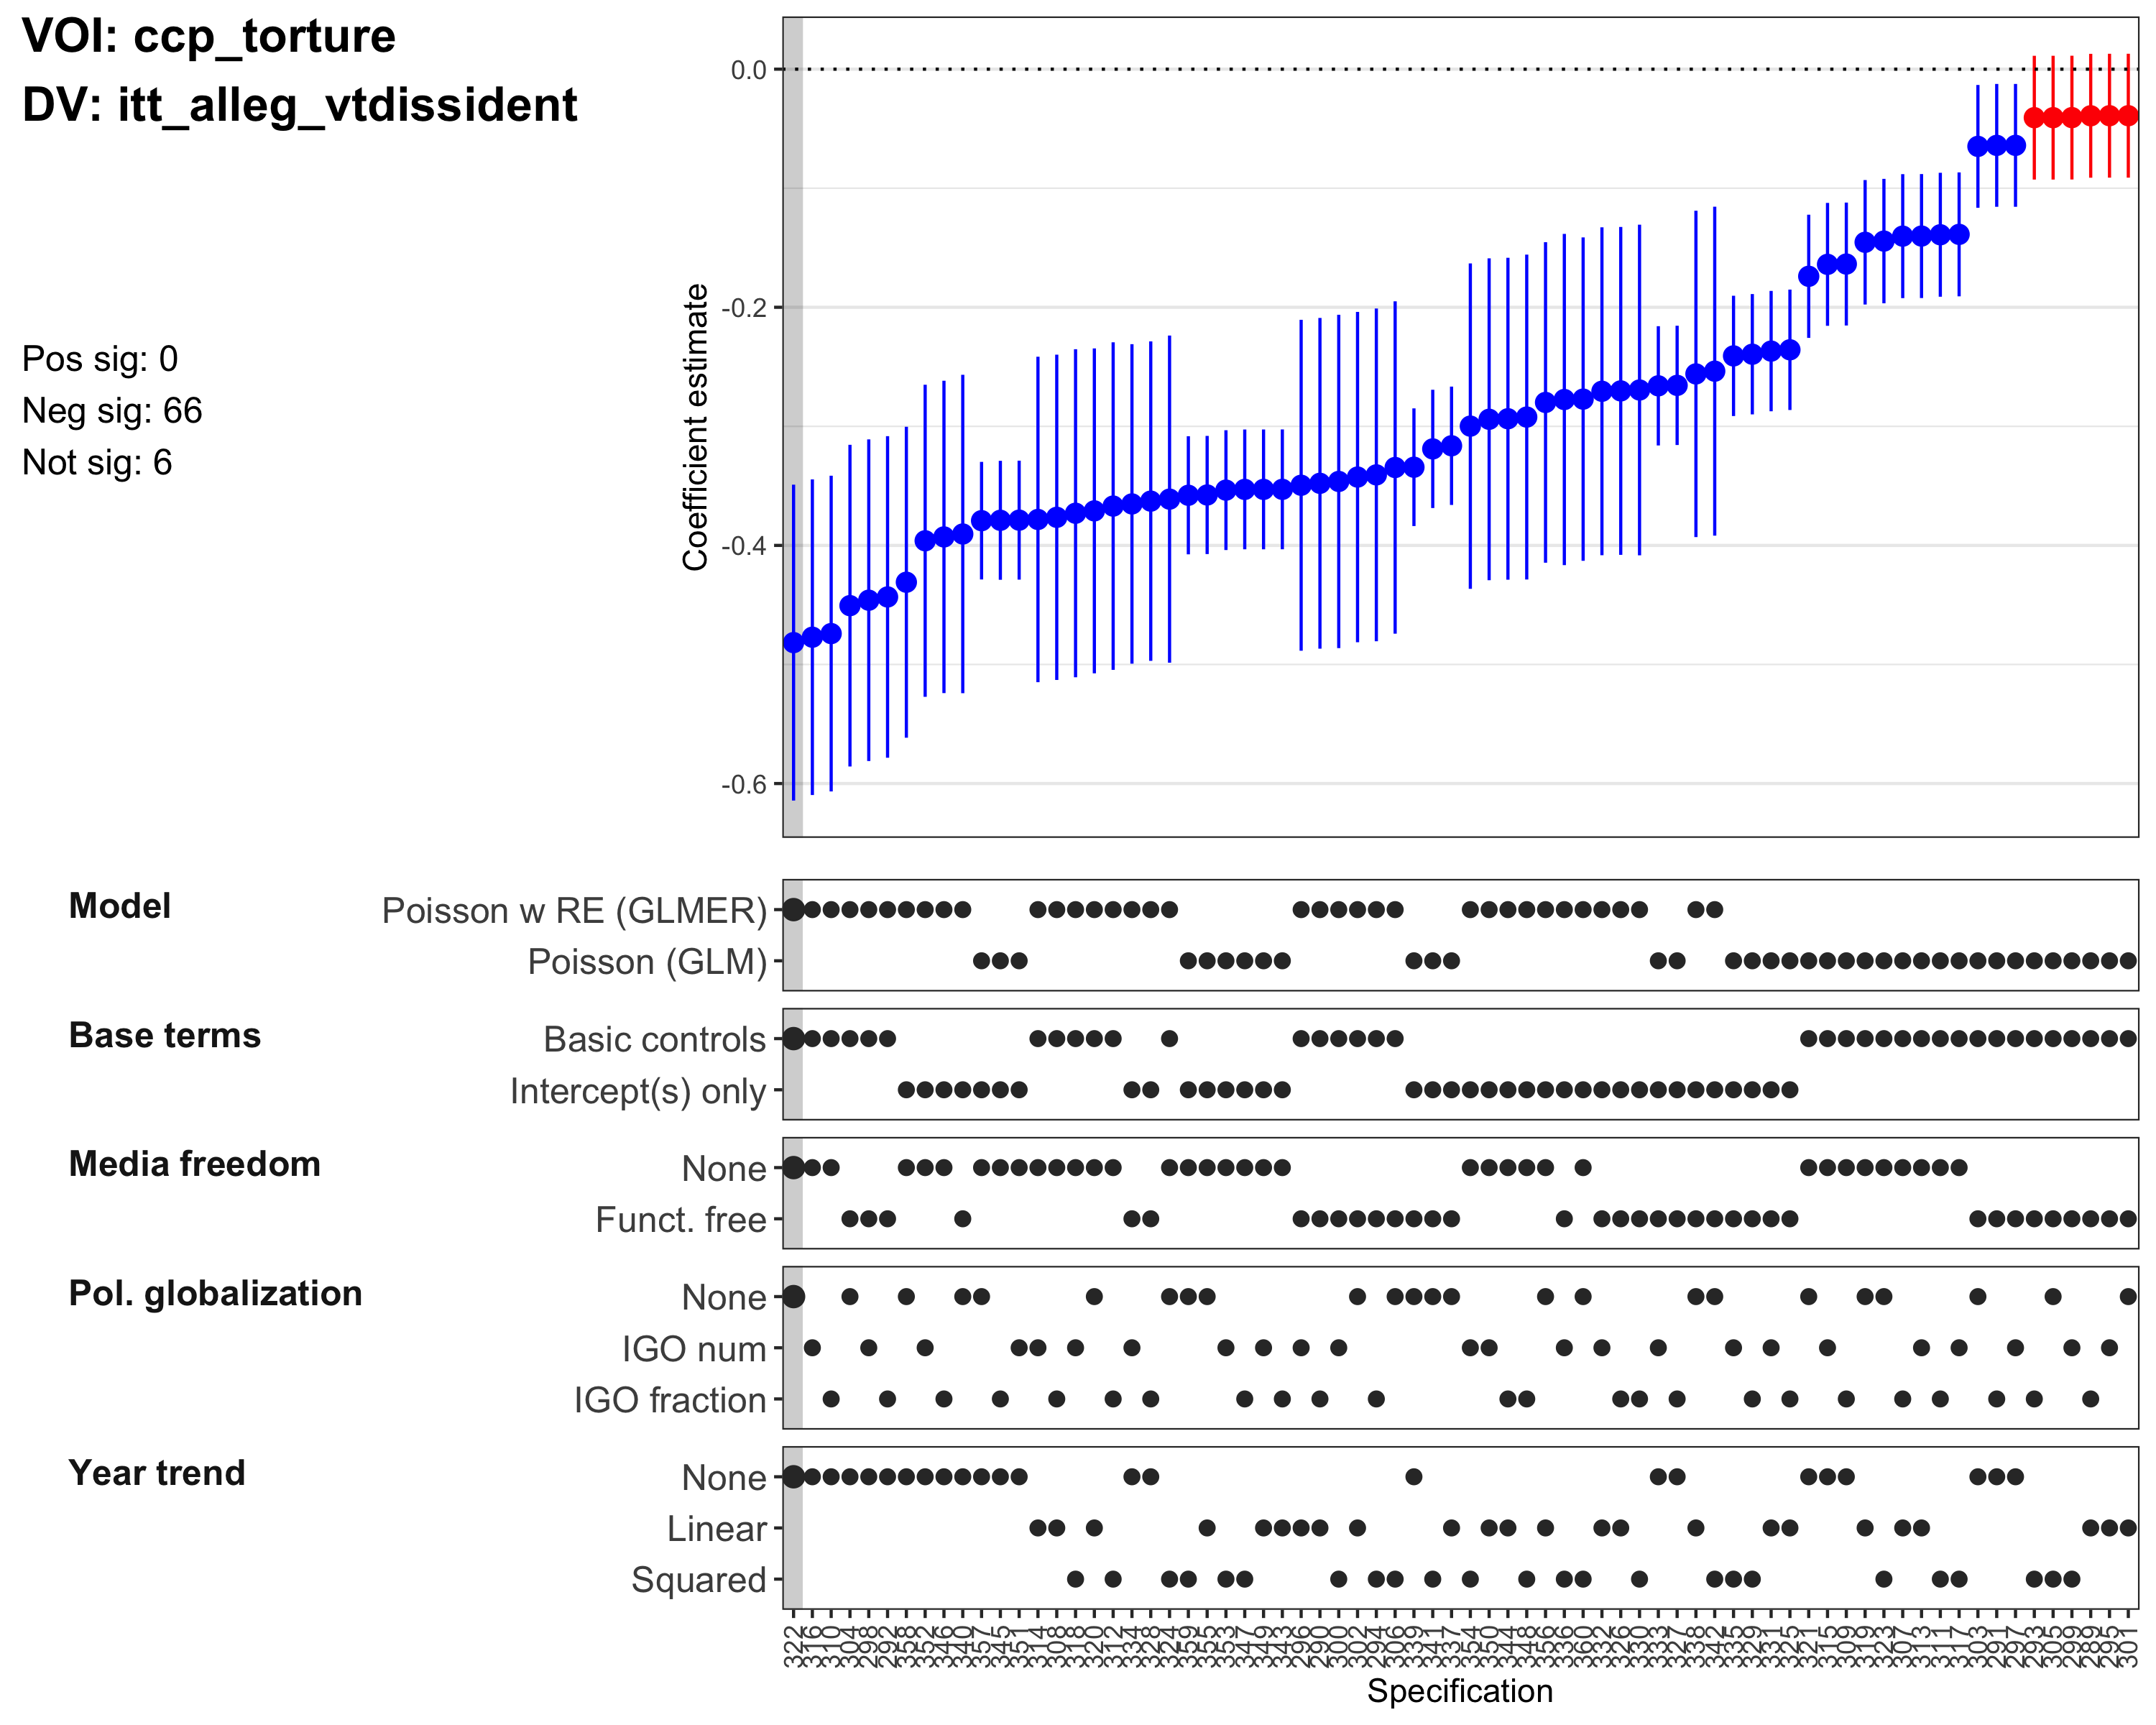
\includegraphics[height=4in]{../output/figures-robustness/specplot-ccp_torture-itt_alleg_vtdissident.png}

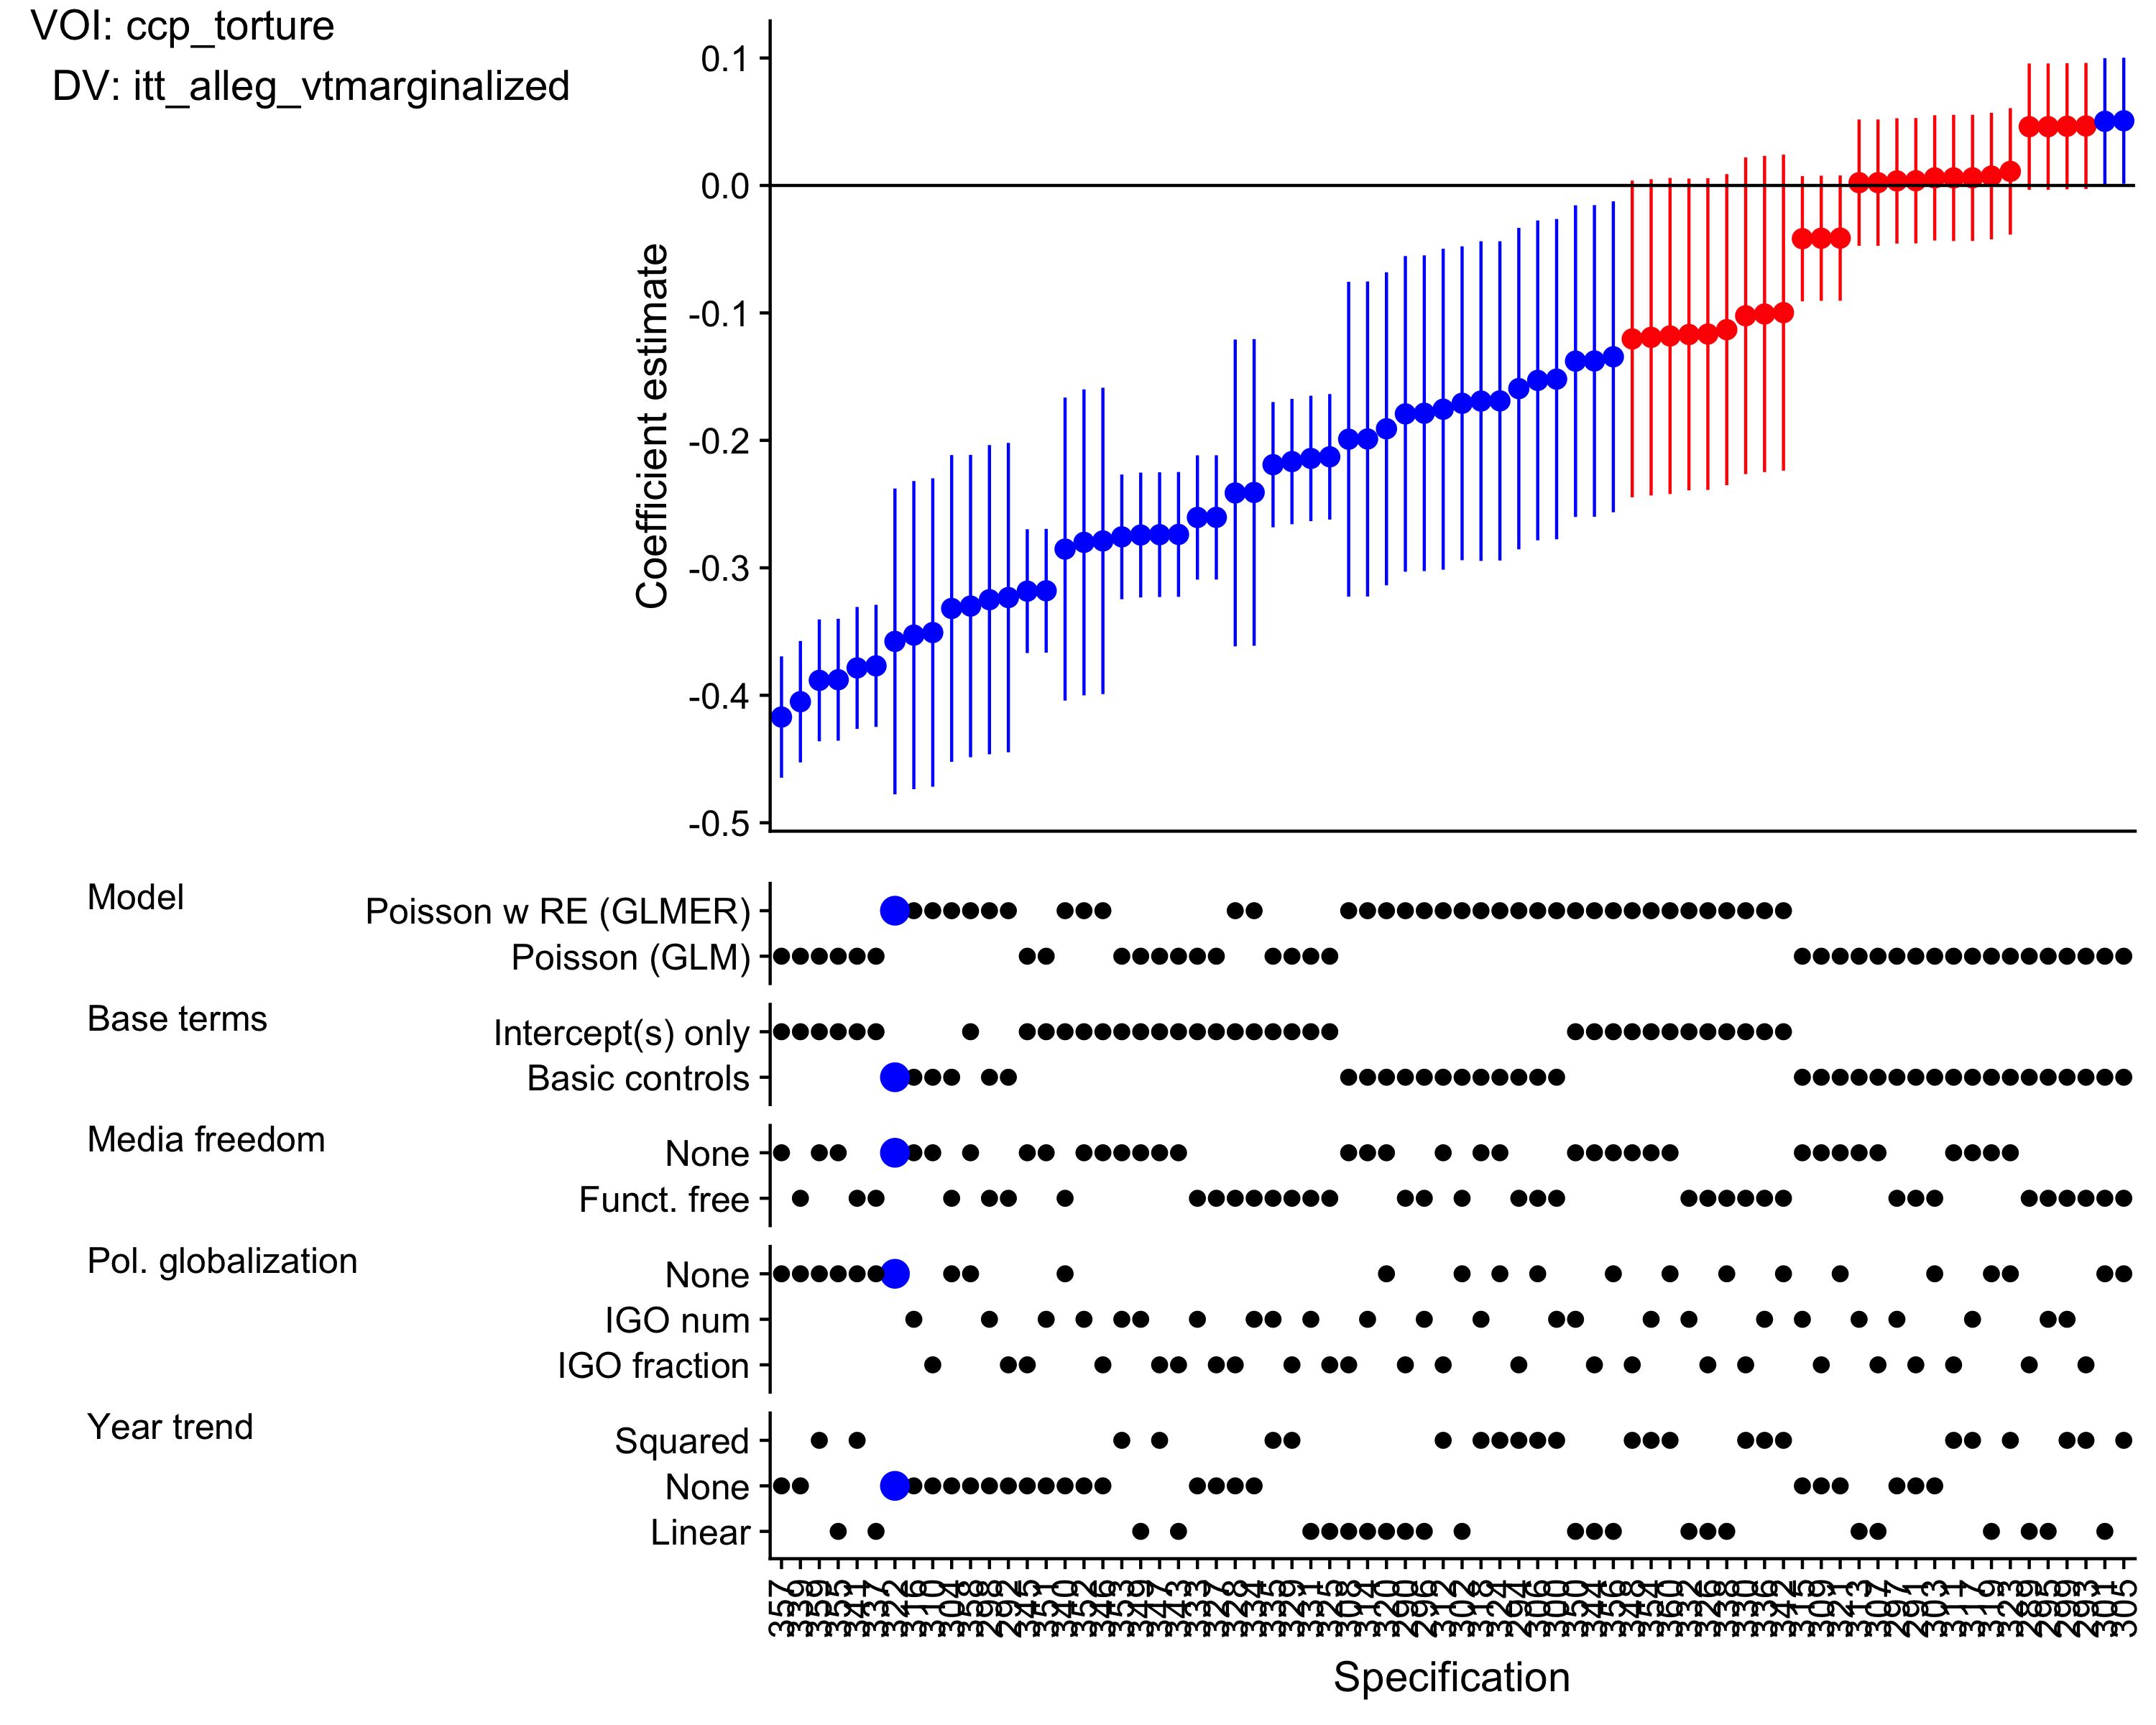
\includegraphics[height=4in]{../output/figures-robustness/specplot-ccp_torture-itt_alleg_vtmarginalized.png}

\hypertarget{voi-dd_democracy}{%
\subsection{VOI: dd\_democracy}\label{voi-dd_democracy}}

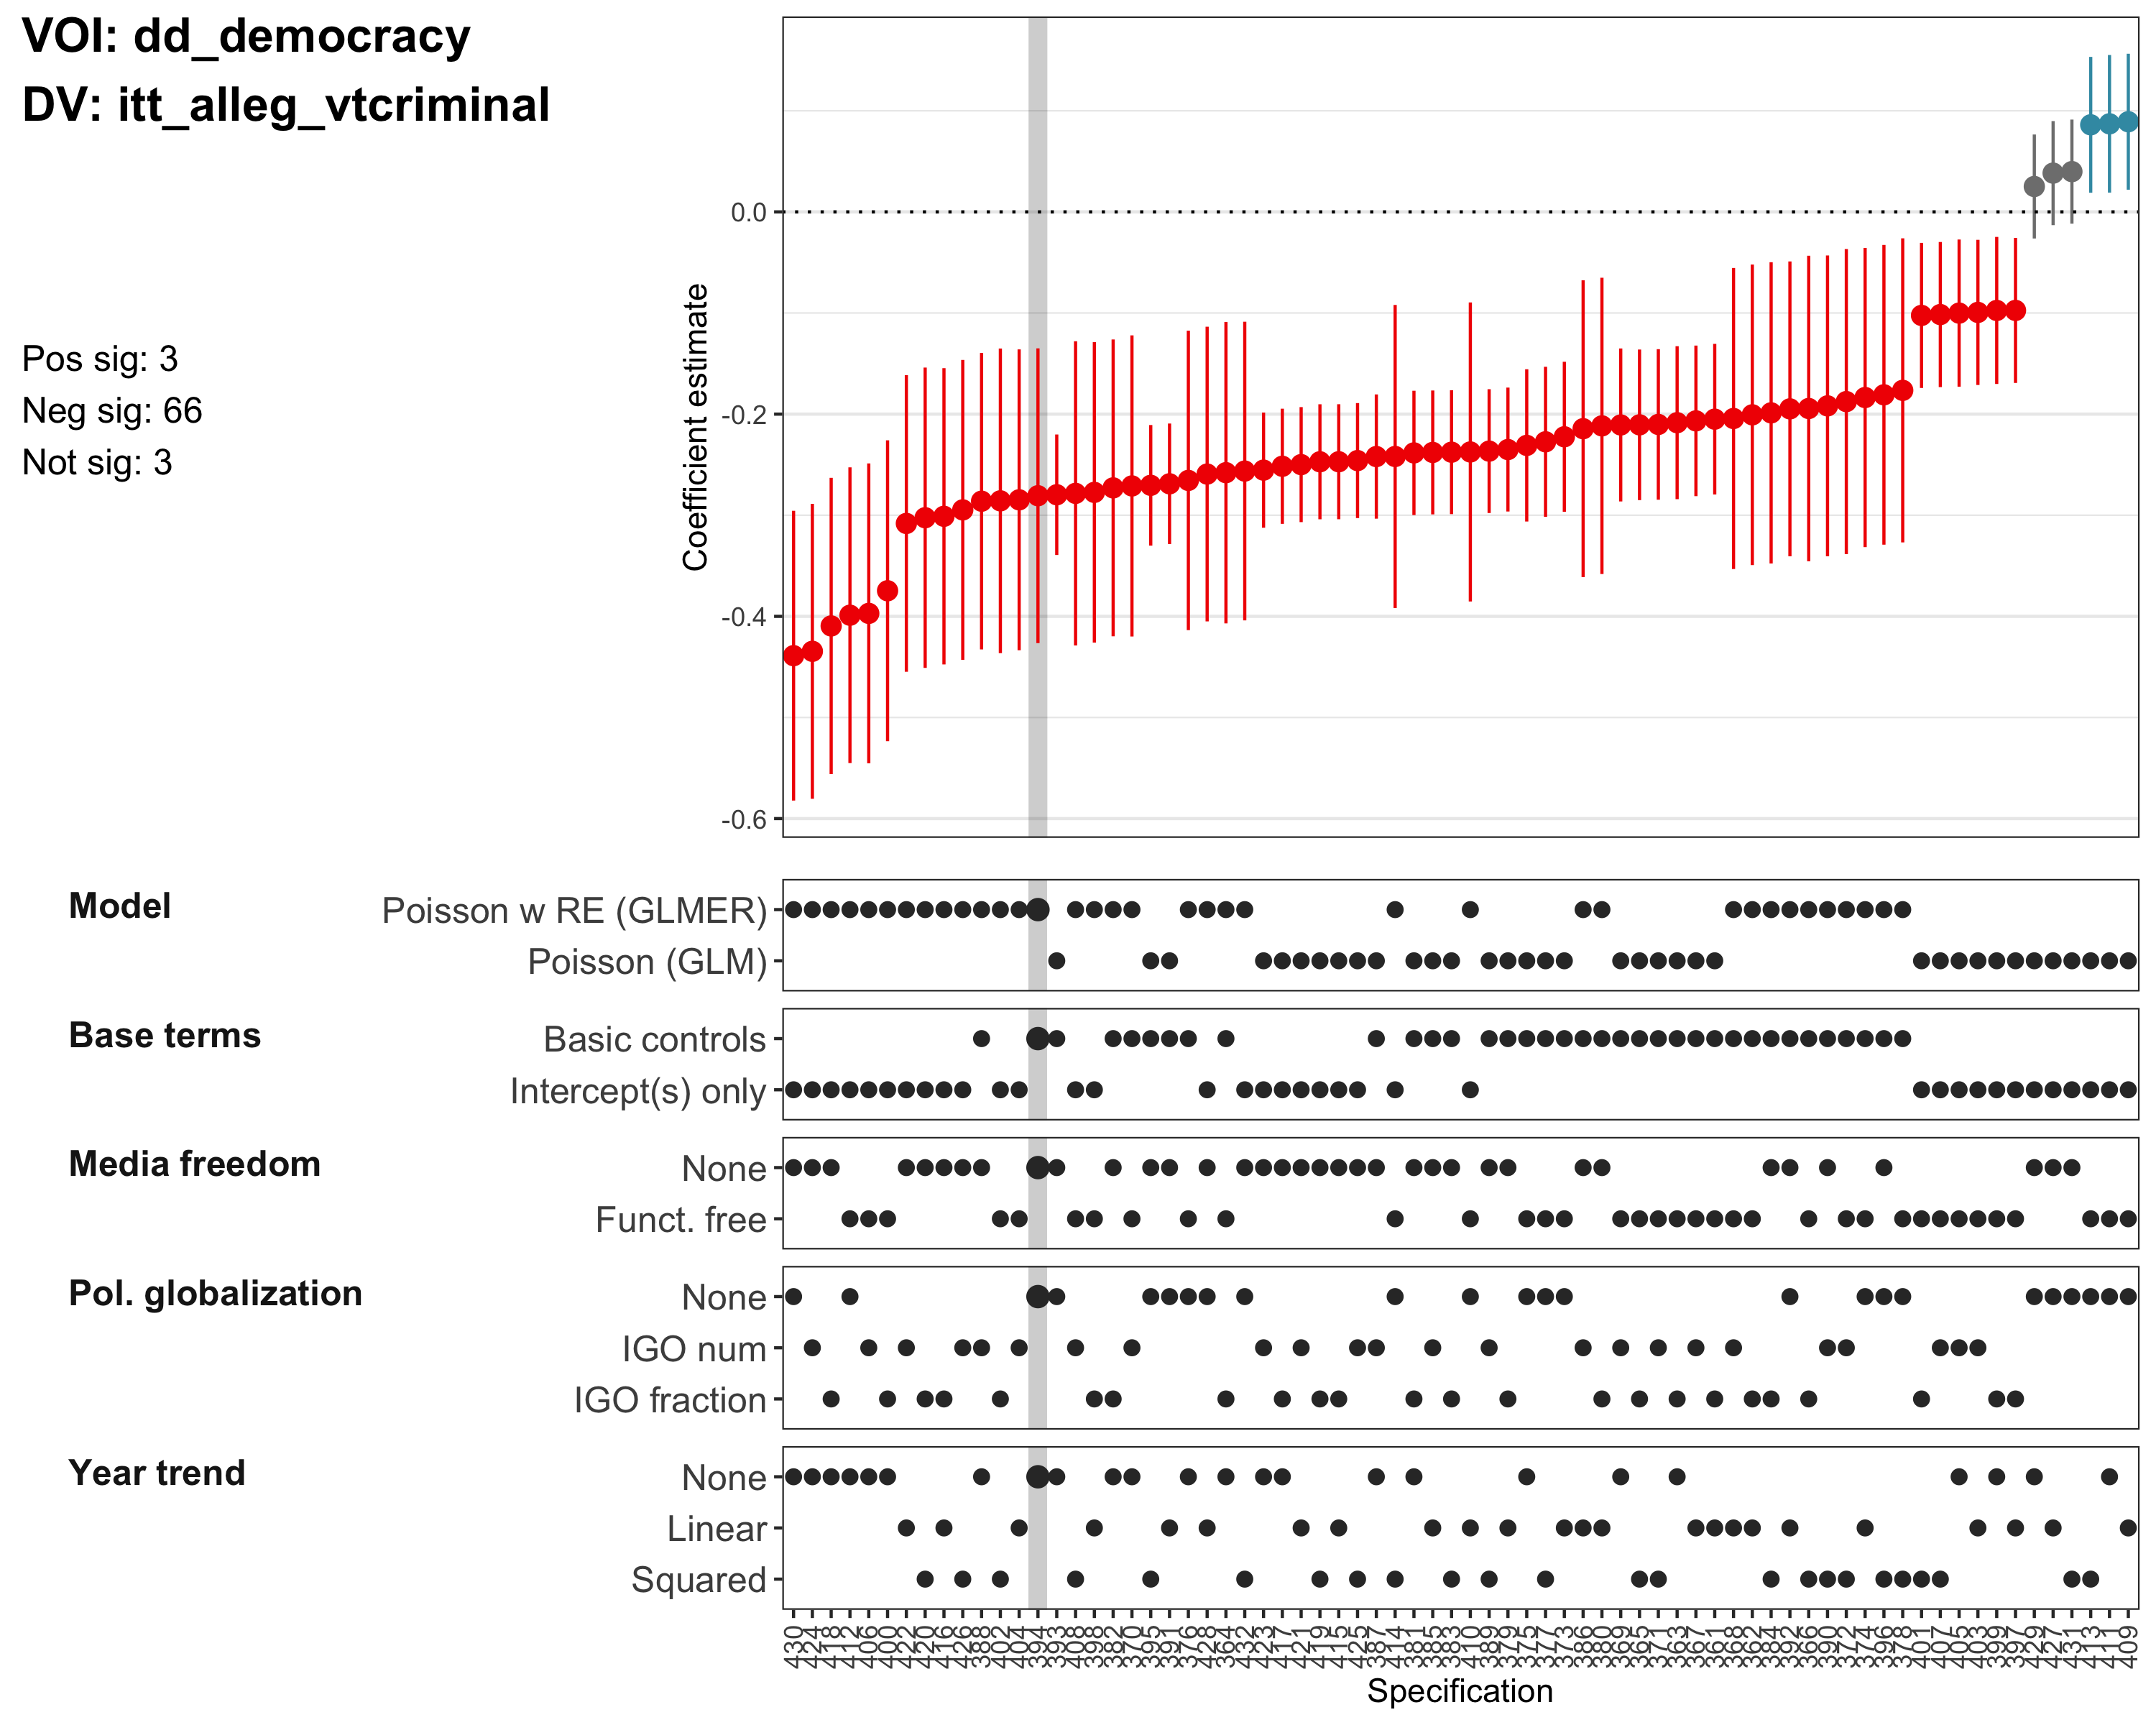
\includegraphics[height=4in]{../output/figures-robustness/specplot-dd_democracy-itt_alleg_vtcriminal.png}

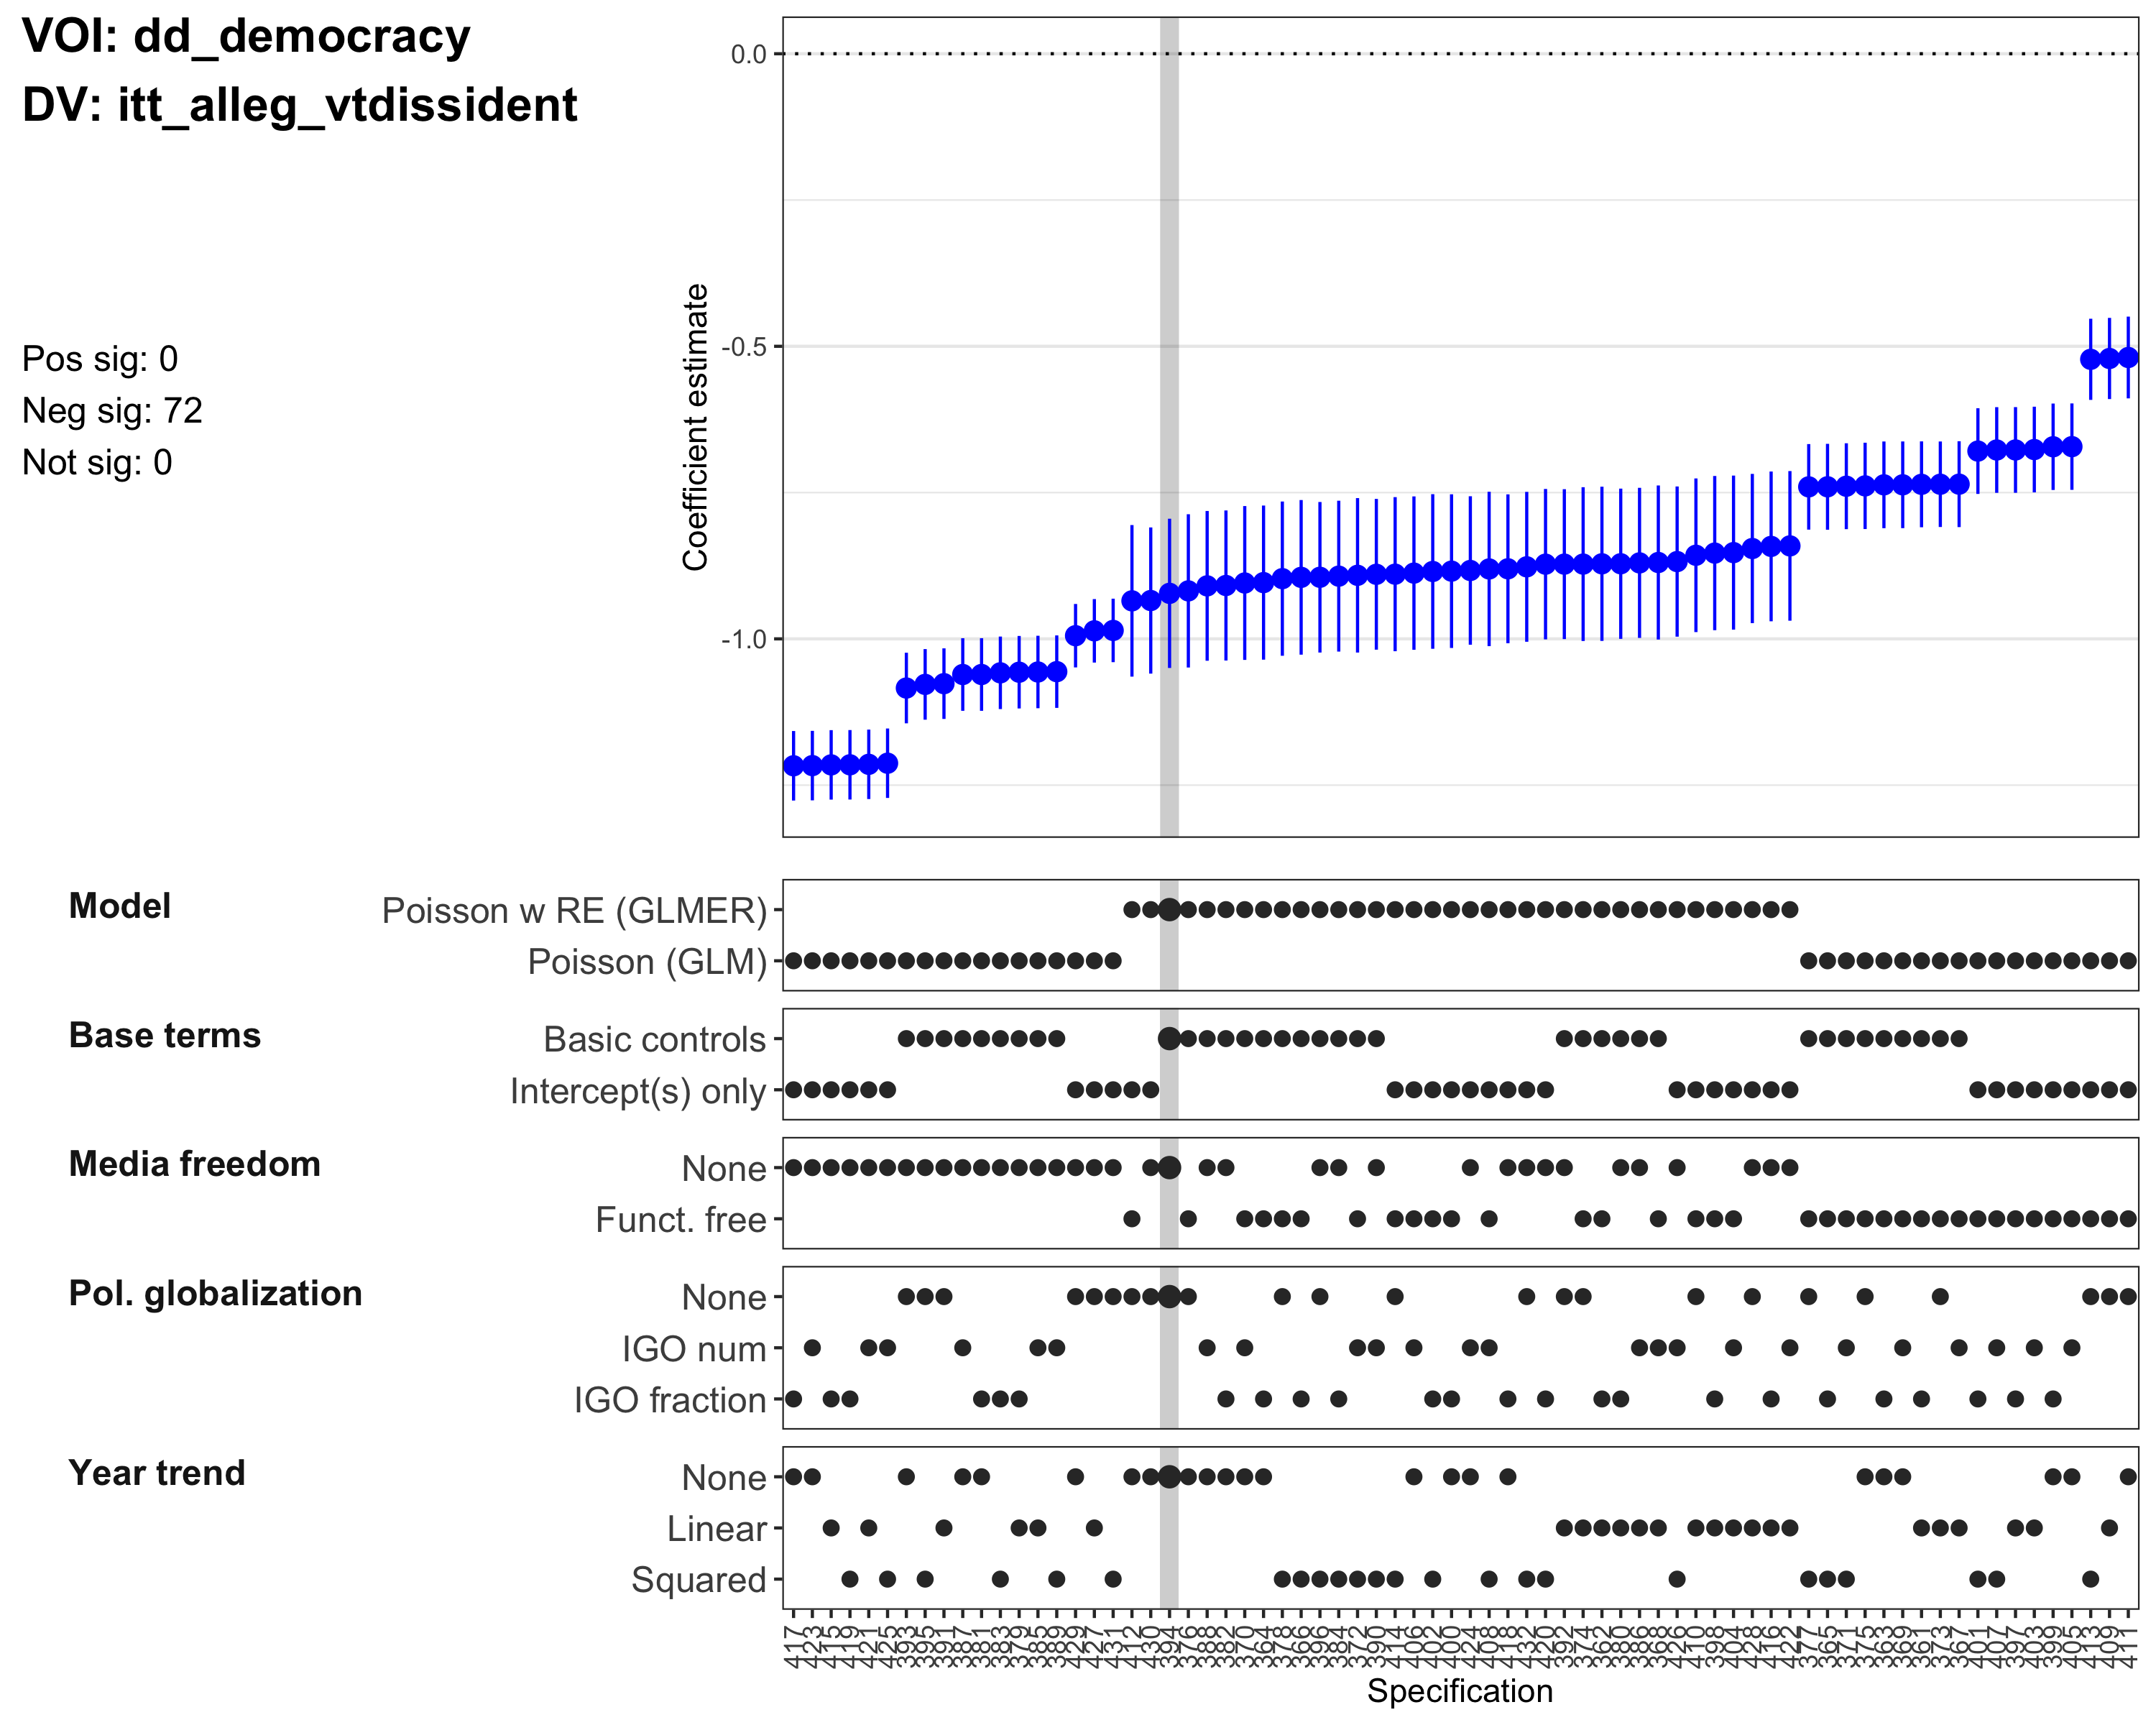
\includegraphics[height=4in]{../output/figures-robustness/specplot-dd_democracy-itt_alleg_vtdissident.png}

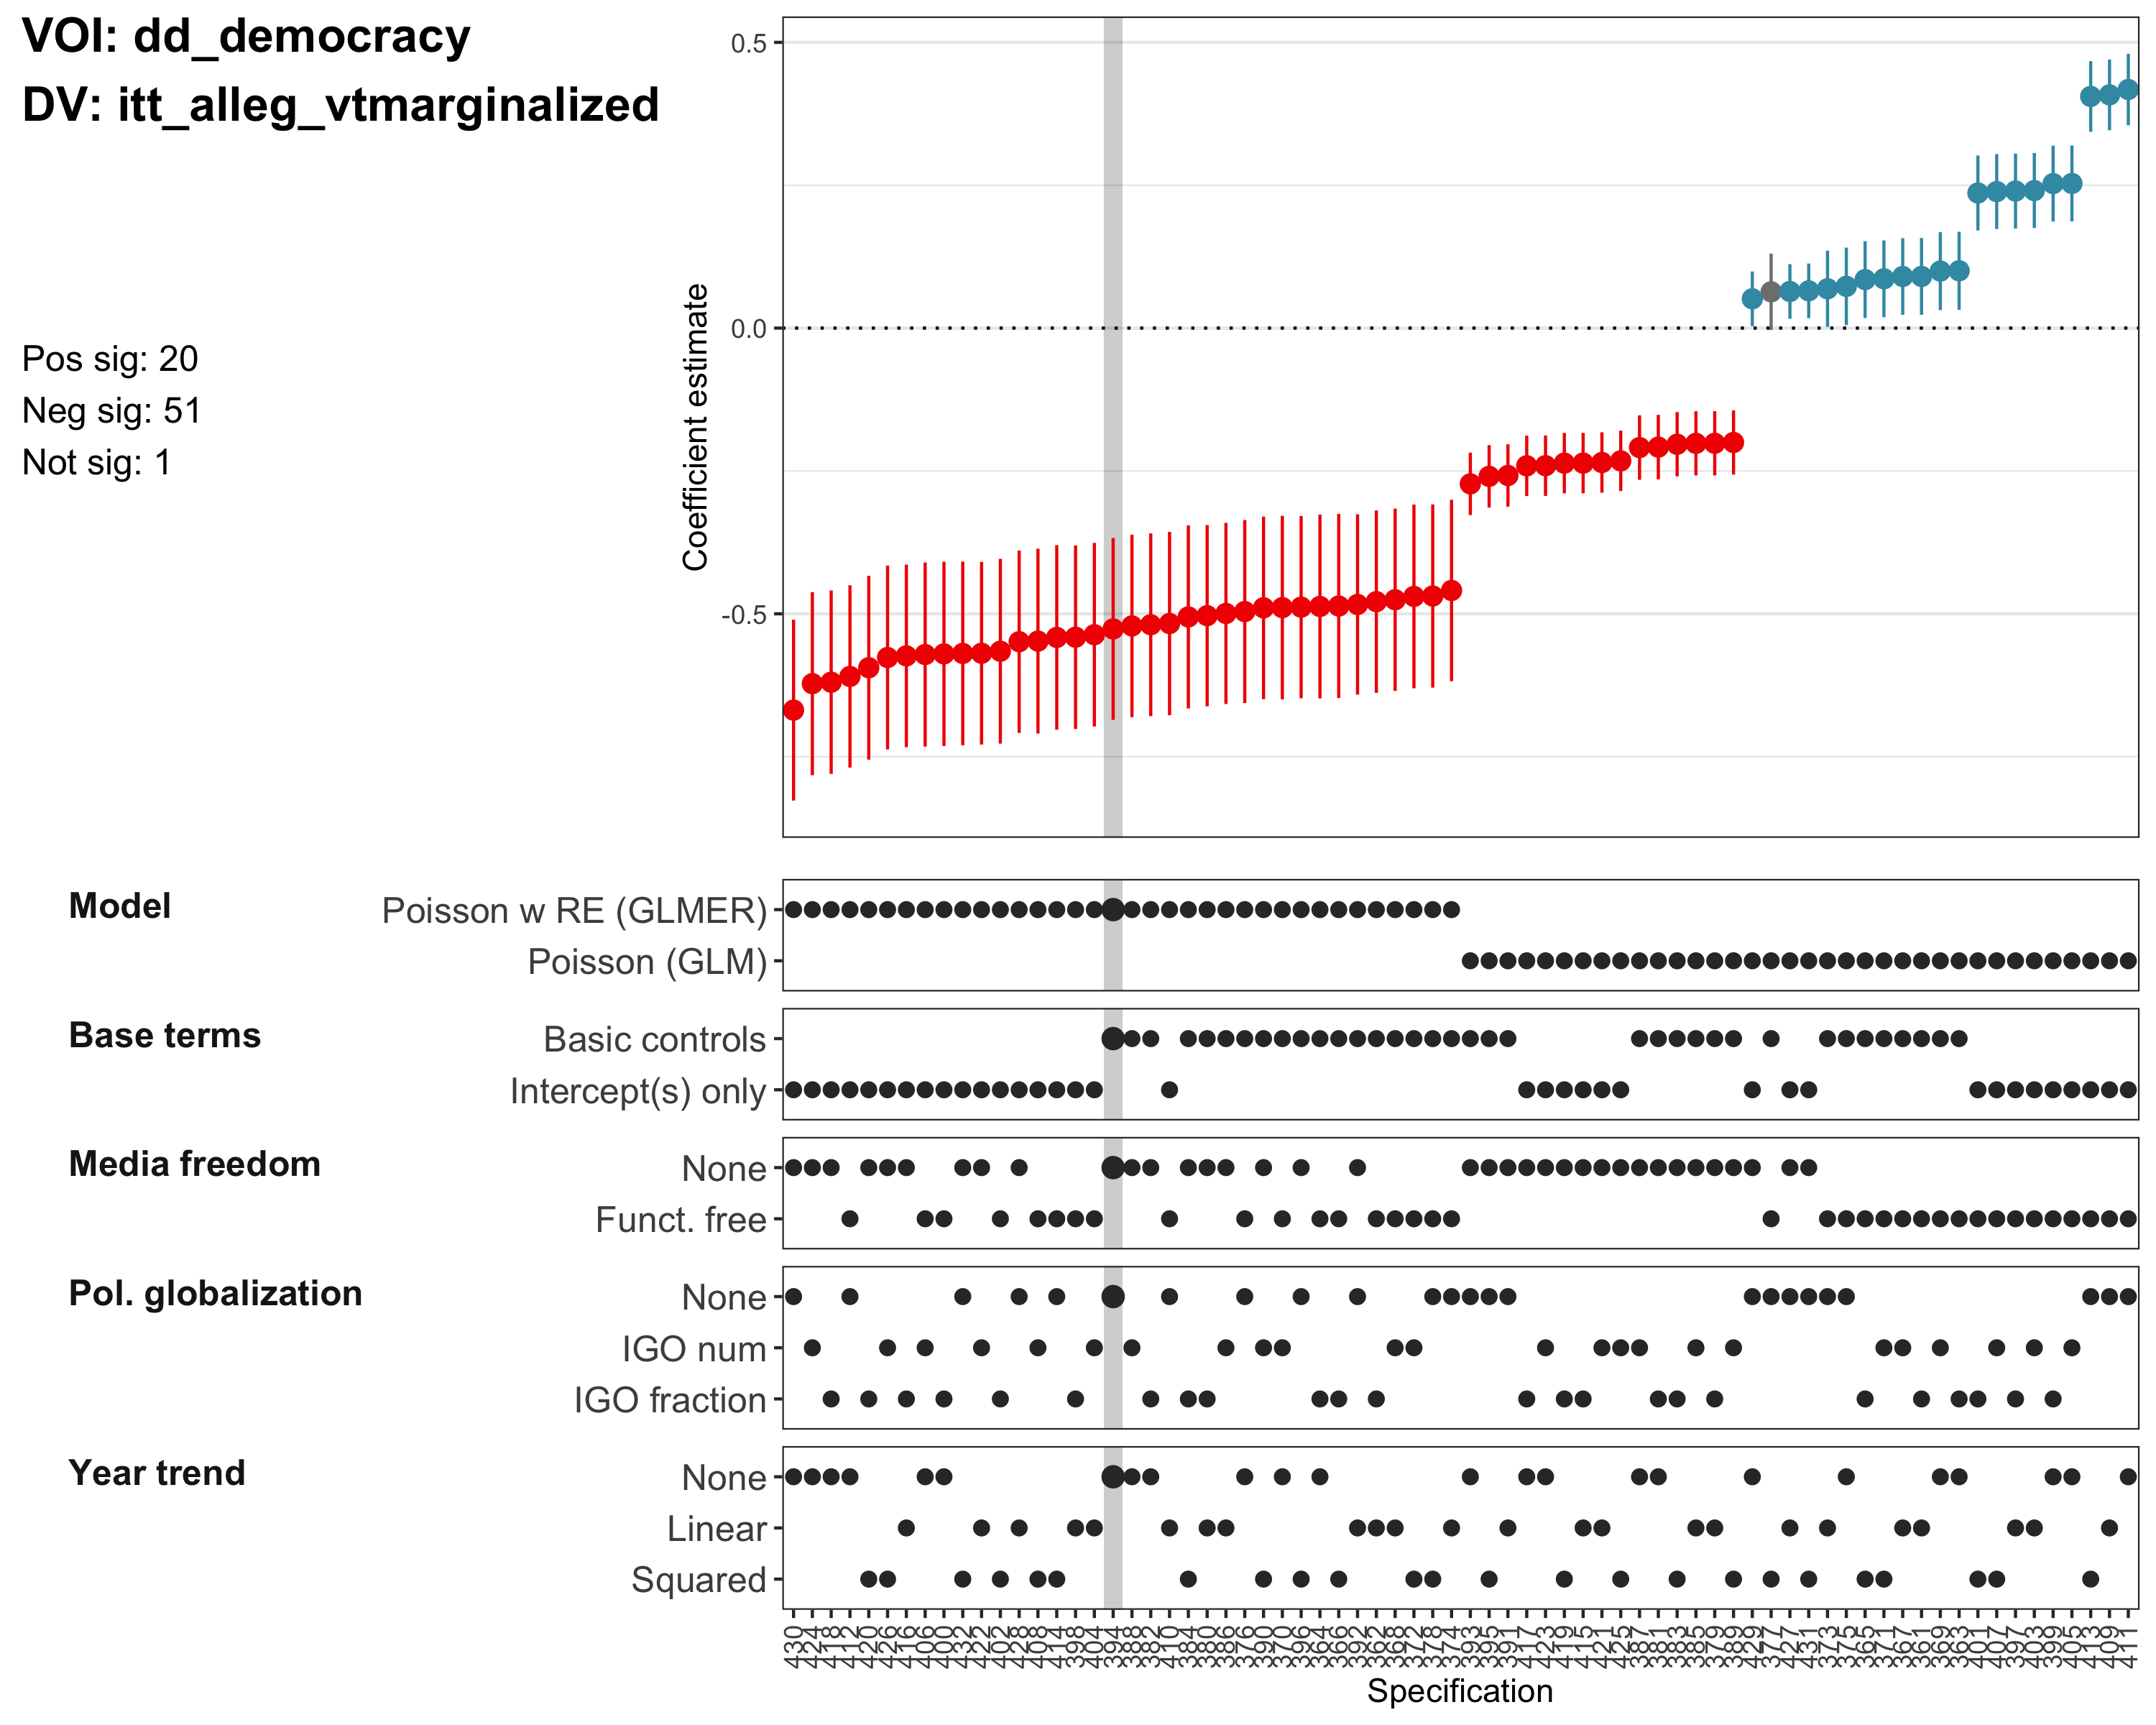
\includegraphics[height=4in]{../output/figures-robustness/specplot-dd_democracy-itt_alleg_vtmarginalized.png}

\hypertarget{voi-epr_excluded_group_pop}{%
\subsection{VOI:
epr\_excluded\_group\_pop}\label{voi-epr_excluded_group_pop}}

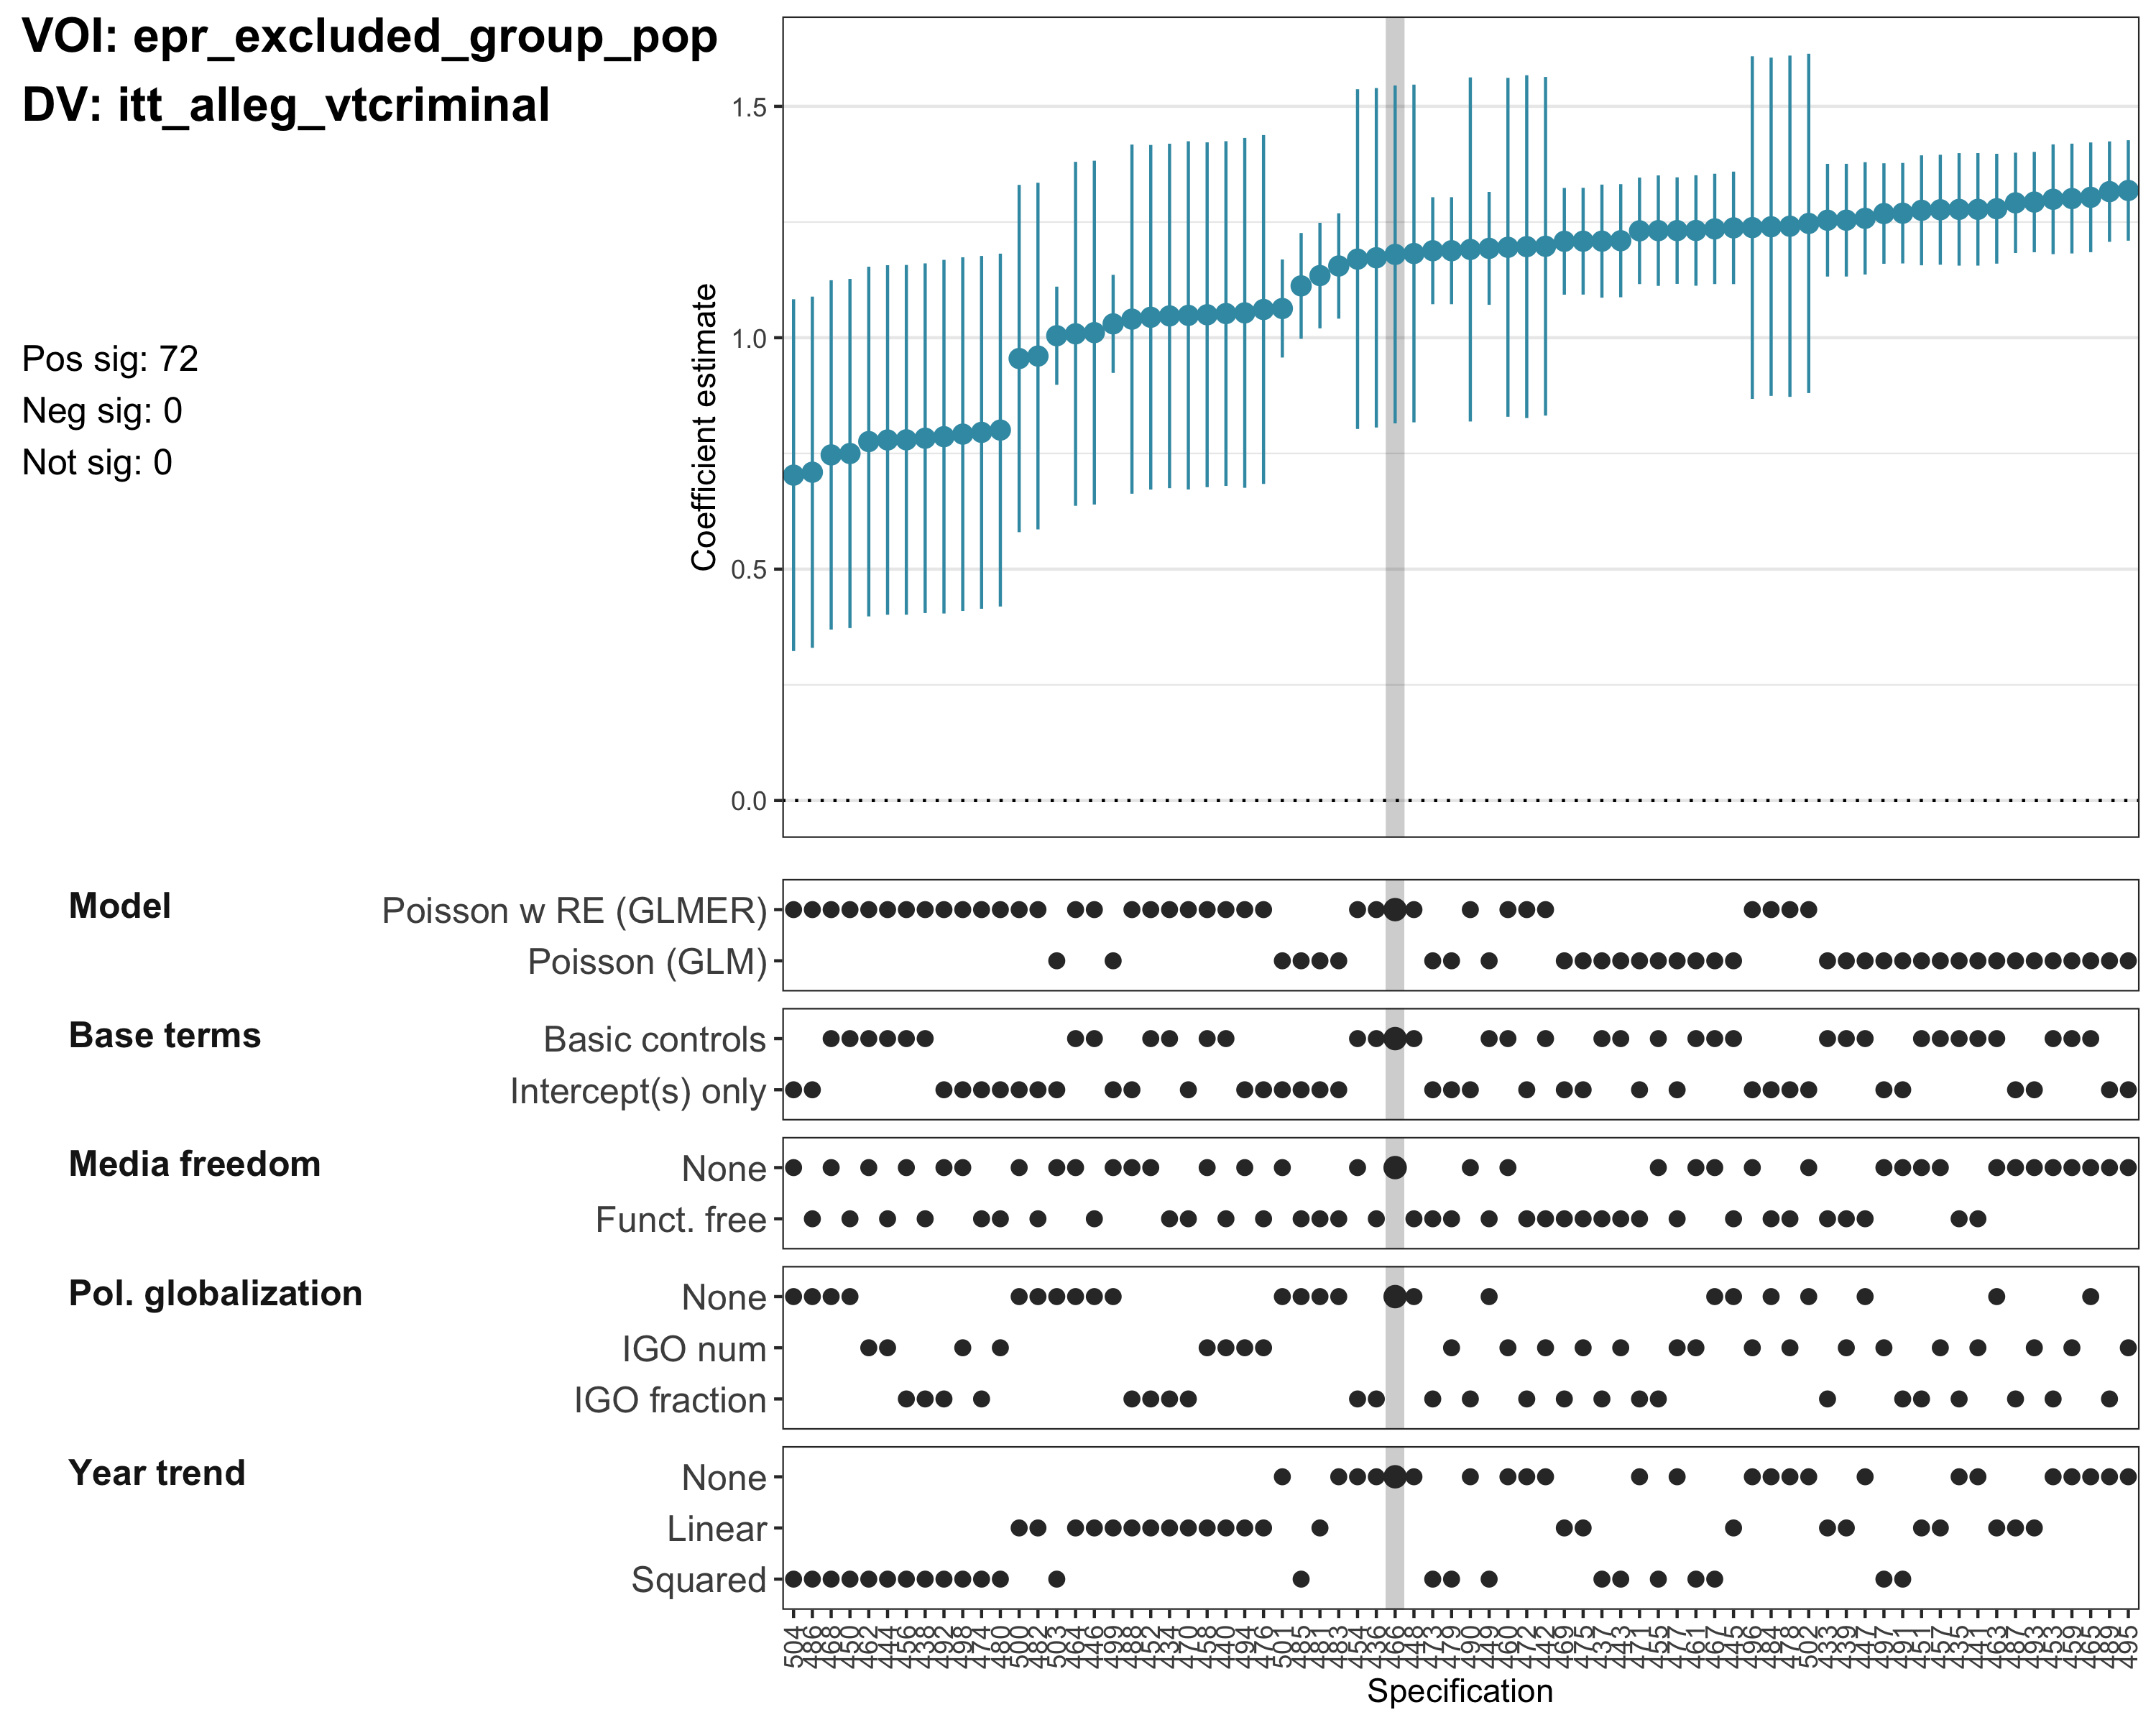
\includegraphics[height=4in]{../output/figures-robustness/specplot-epr_excluded_group_pop-itt_alleg_vtcriminal.png}

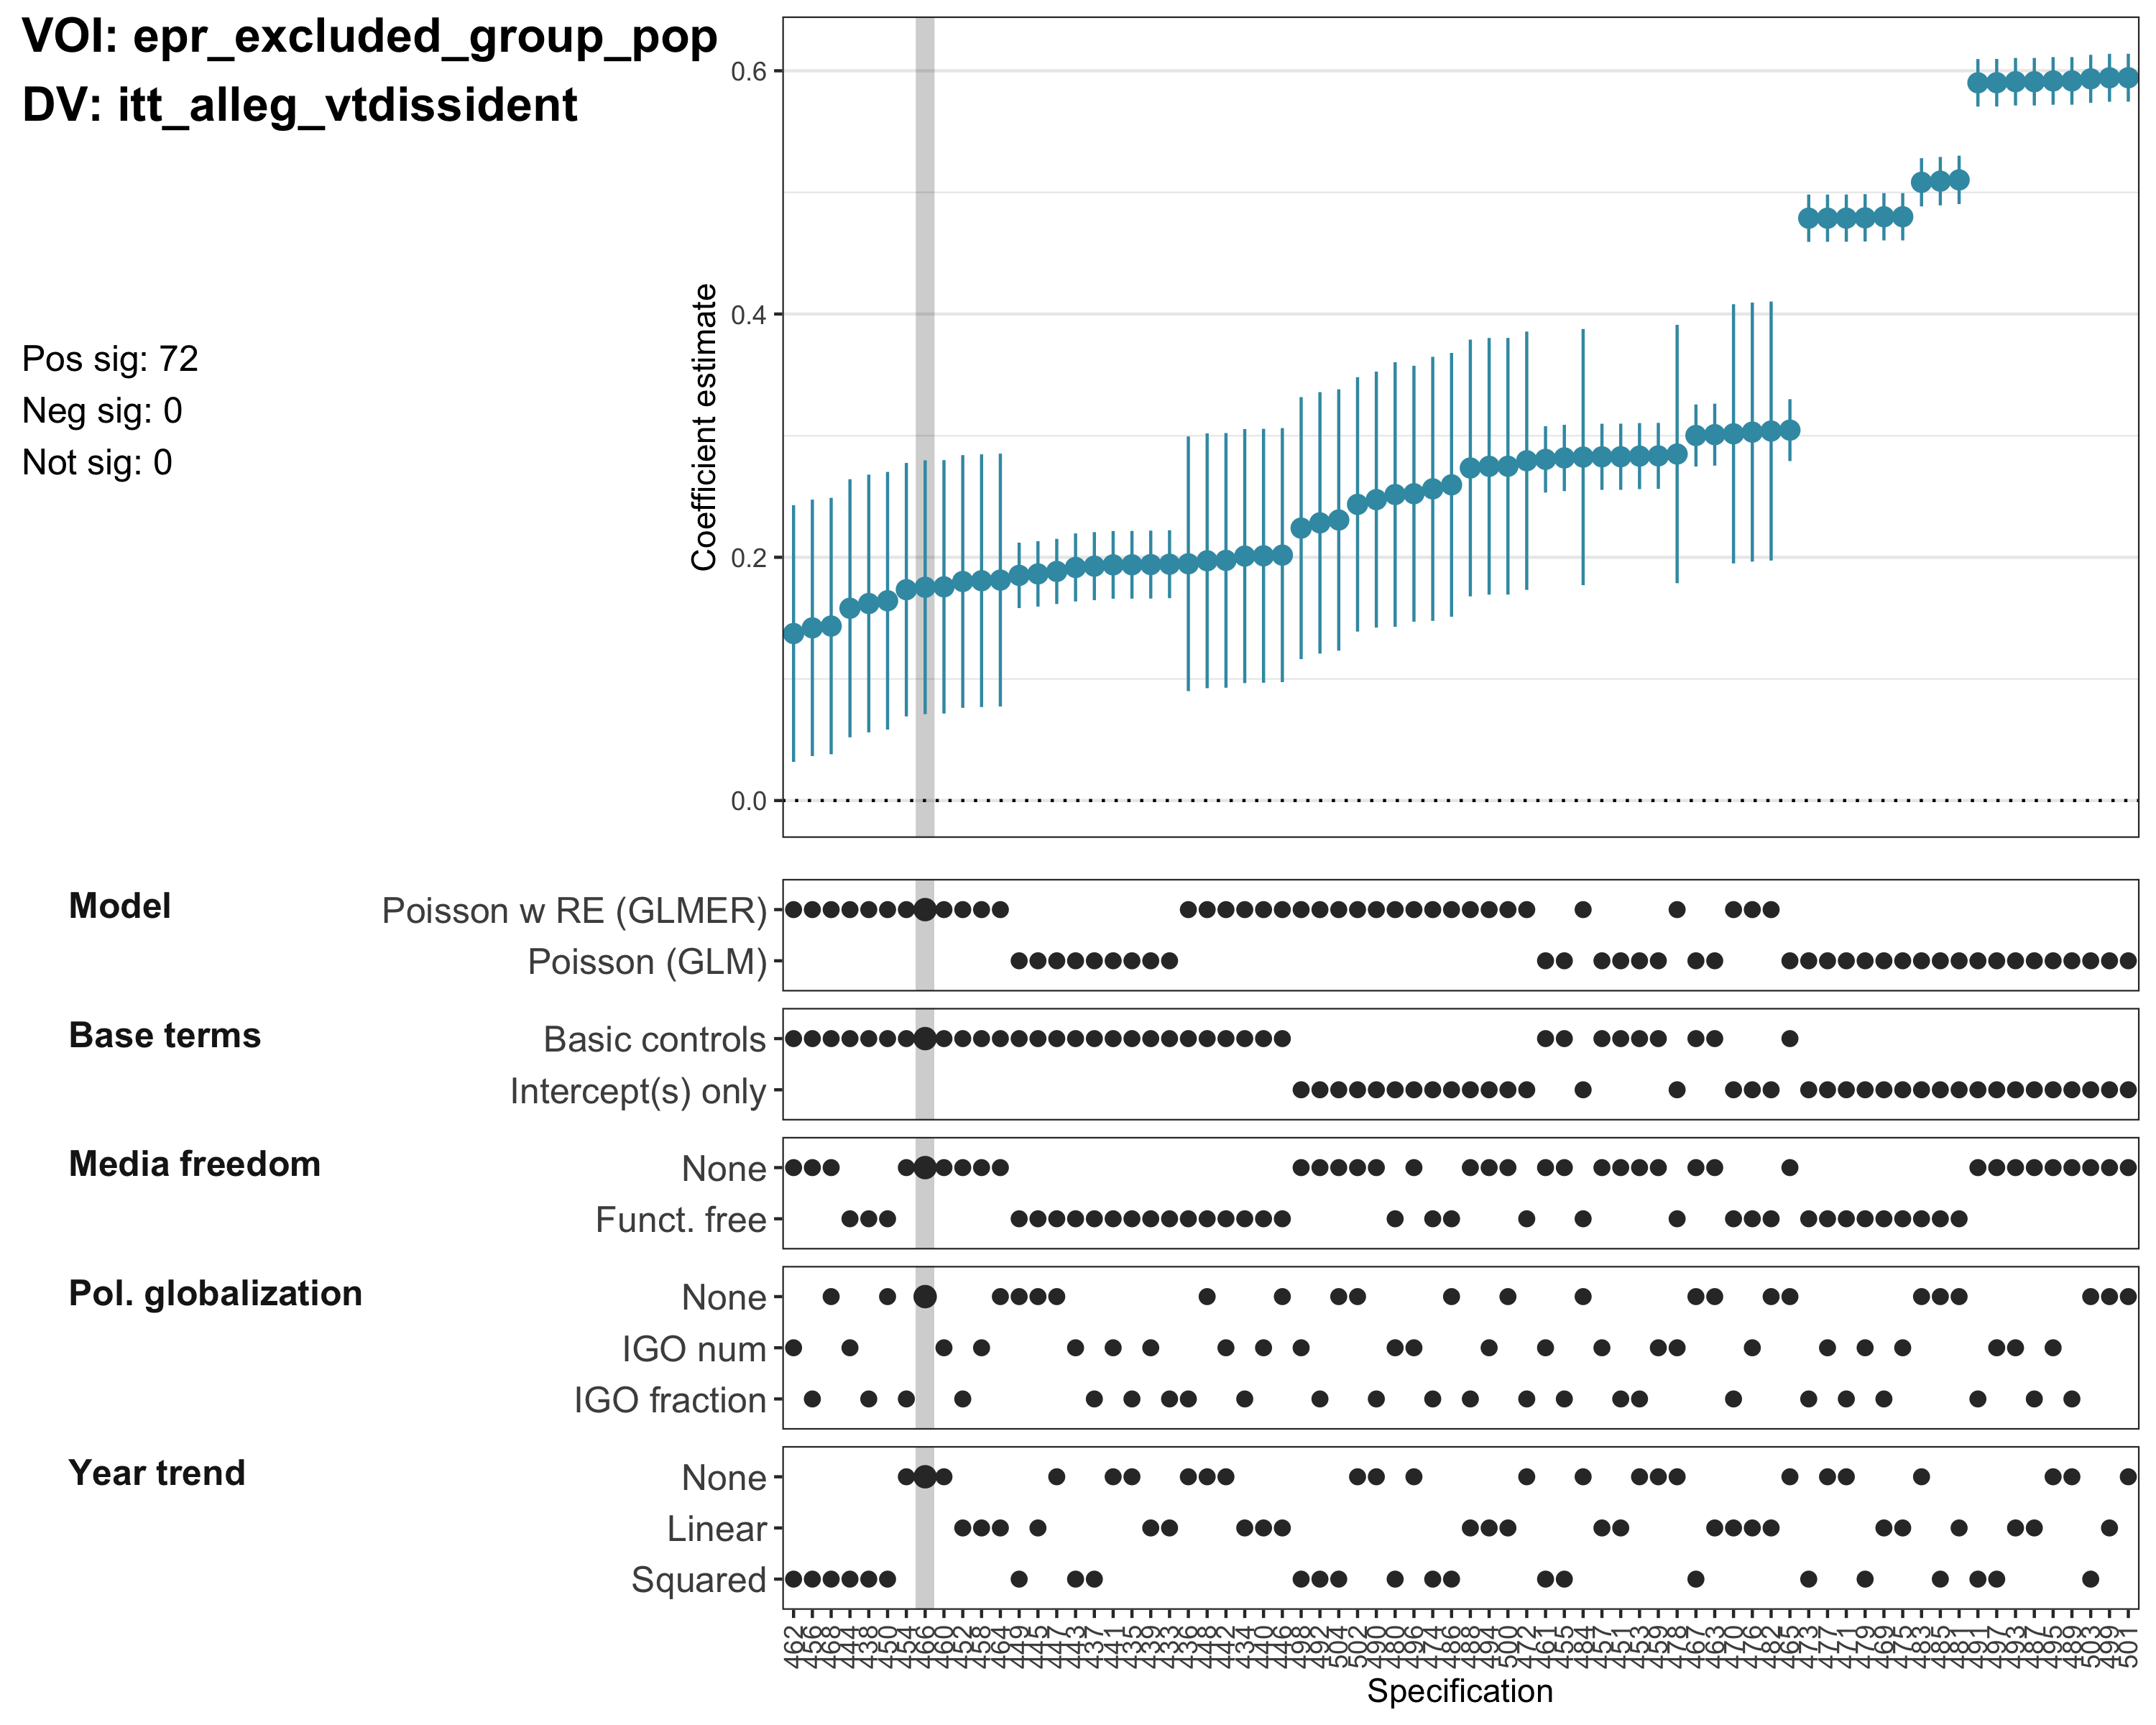
\includegraphics[height=4in]{../output/figures-robustness/specplot-epr_excluded_group_pop-itt_alleg_vtdissident.png}

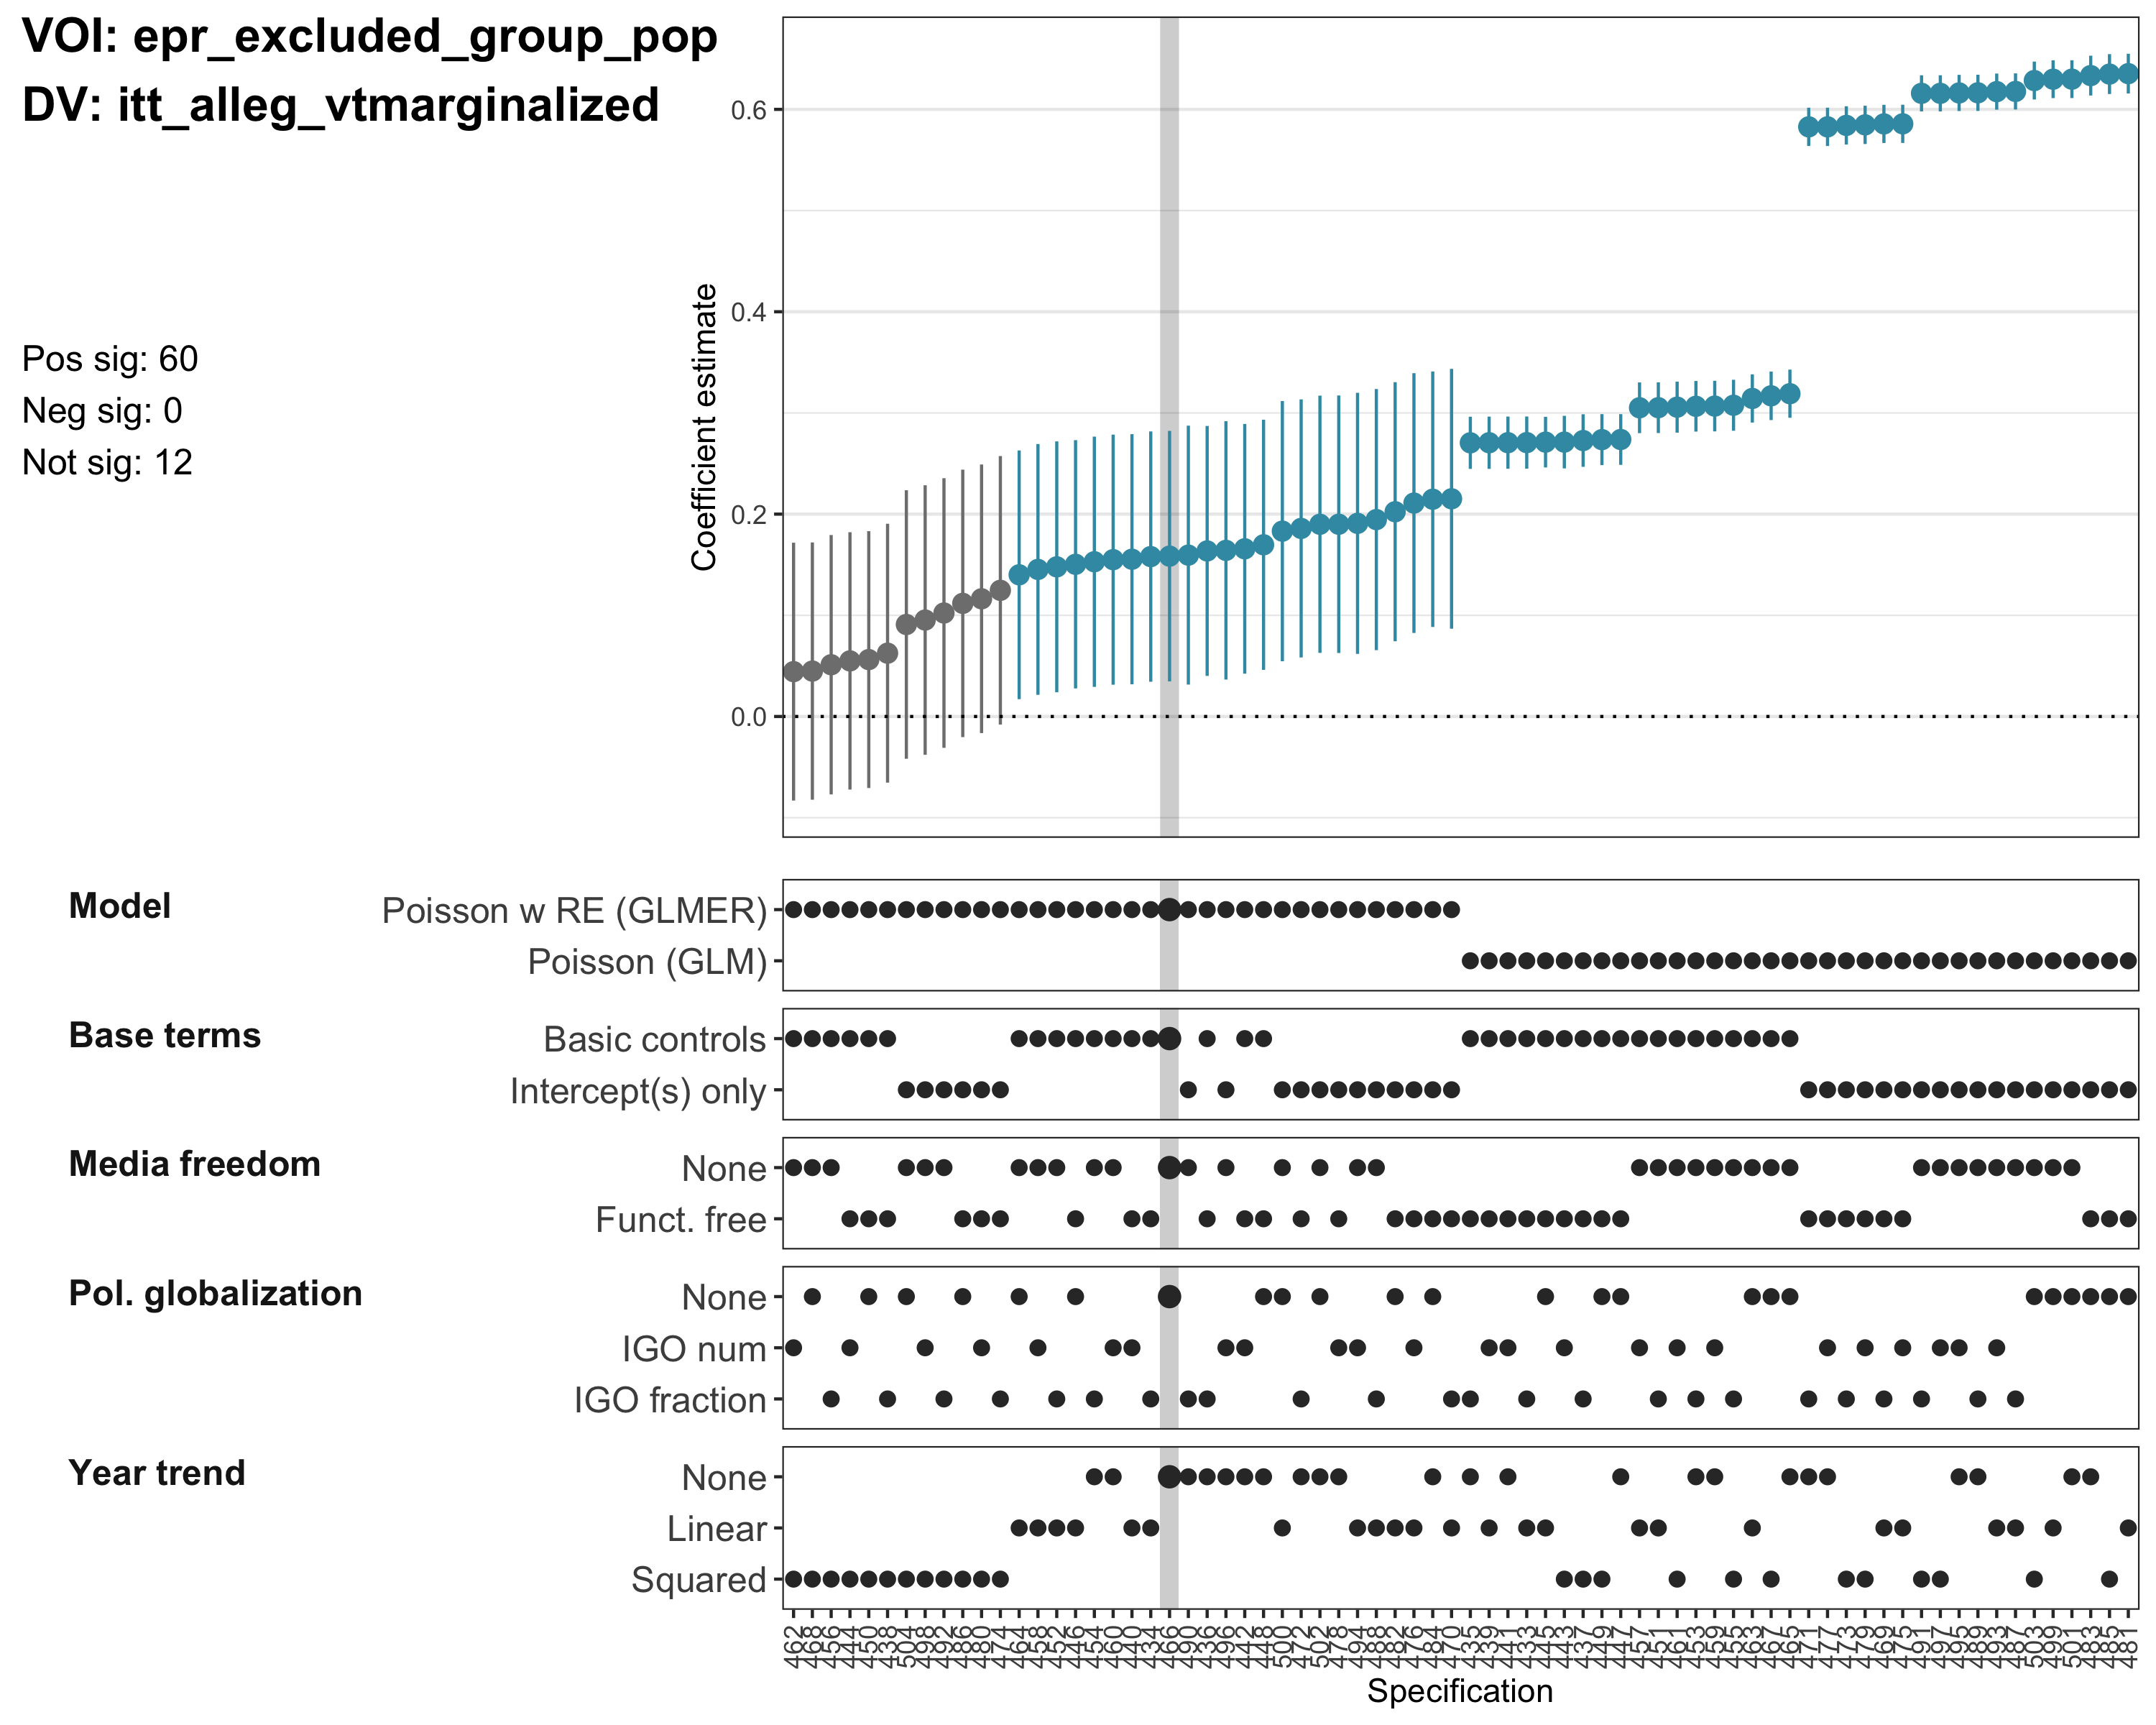
\includegraphics[height=4in]{../output/figures-robustness/specplot-epr_excluded_group_pop-itt_alleg_vtmarginalized.png}

\hypertarget{voi-epr_excluded_groups_count}{%
\subsection{VOI:
epr\_excluded\_groups\_count}\label{voi-epr_excluded_groups_count}}

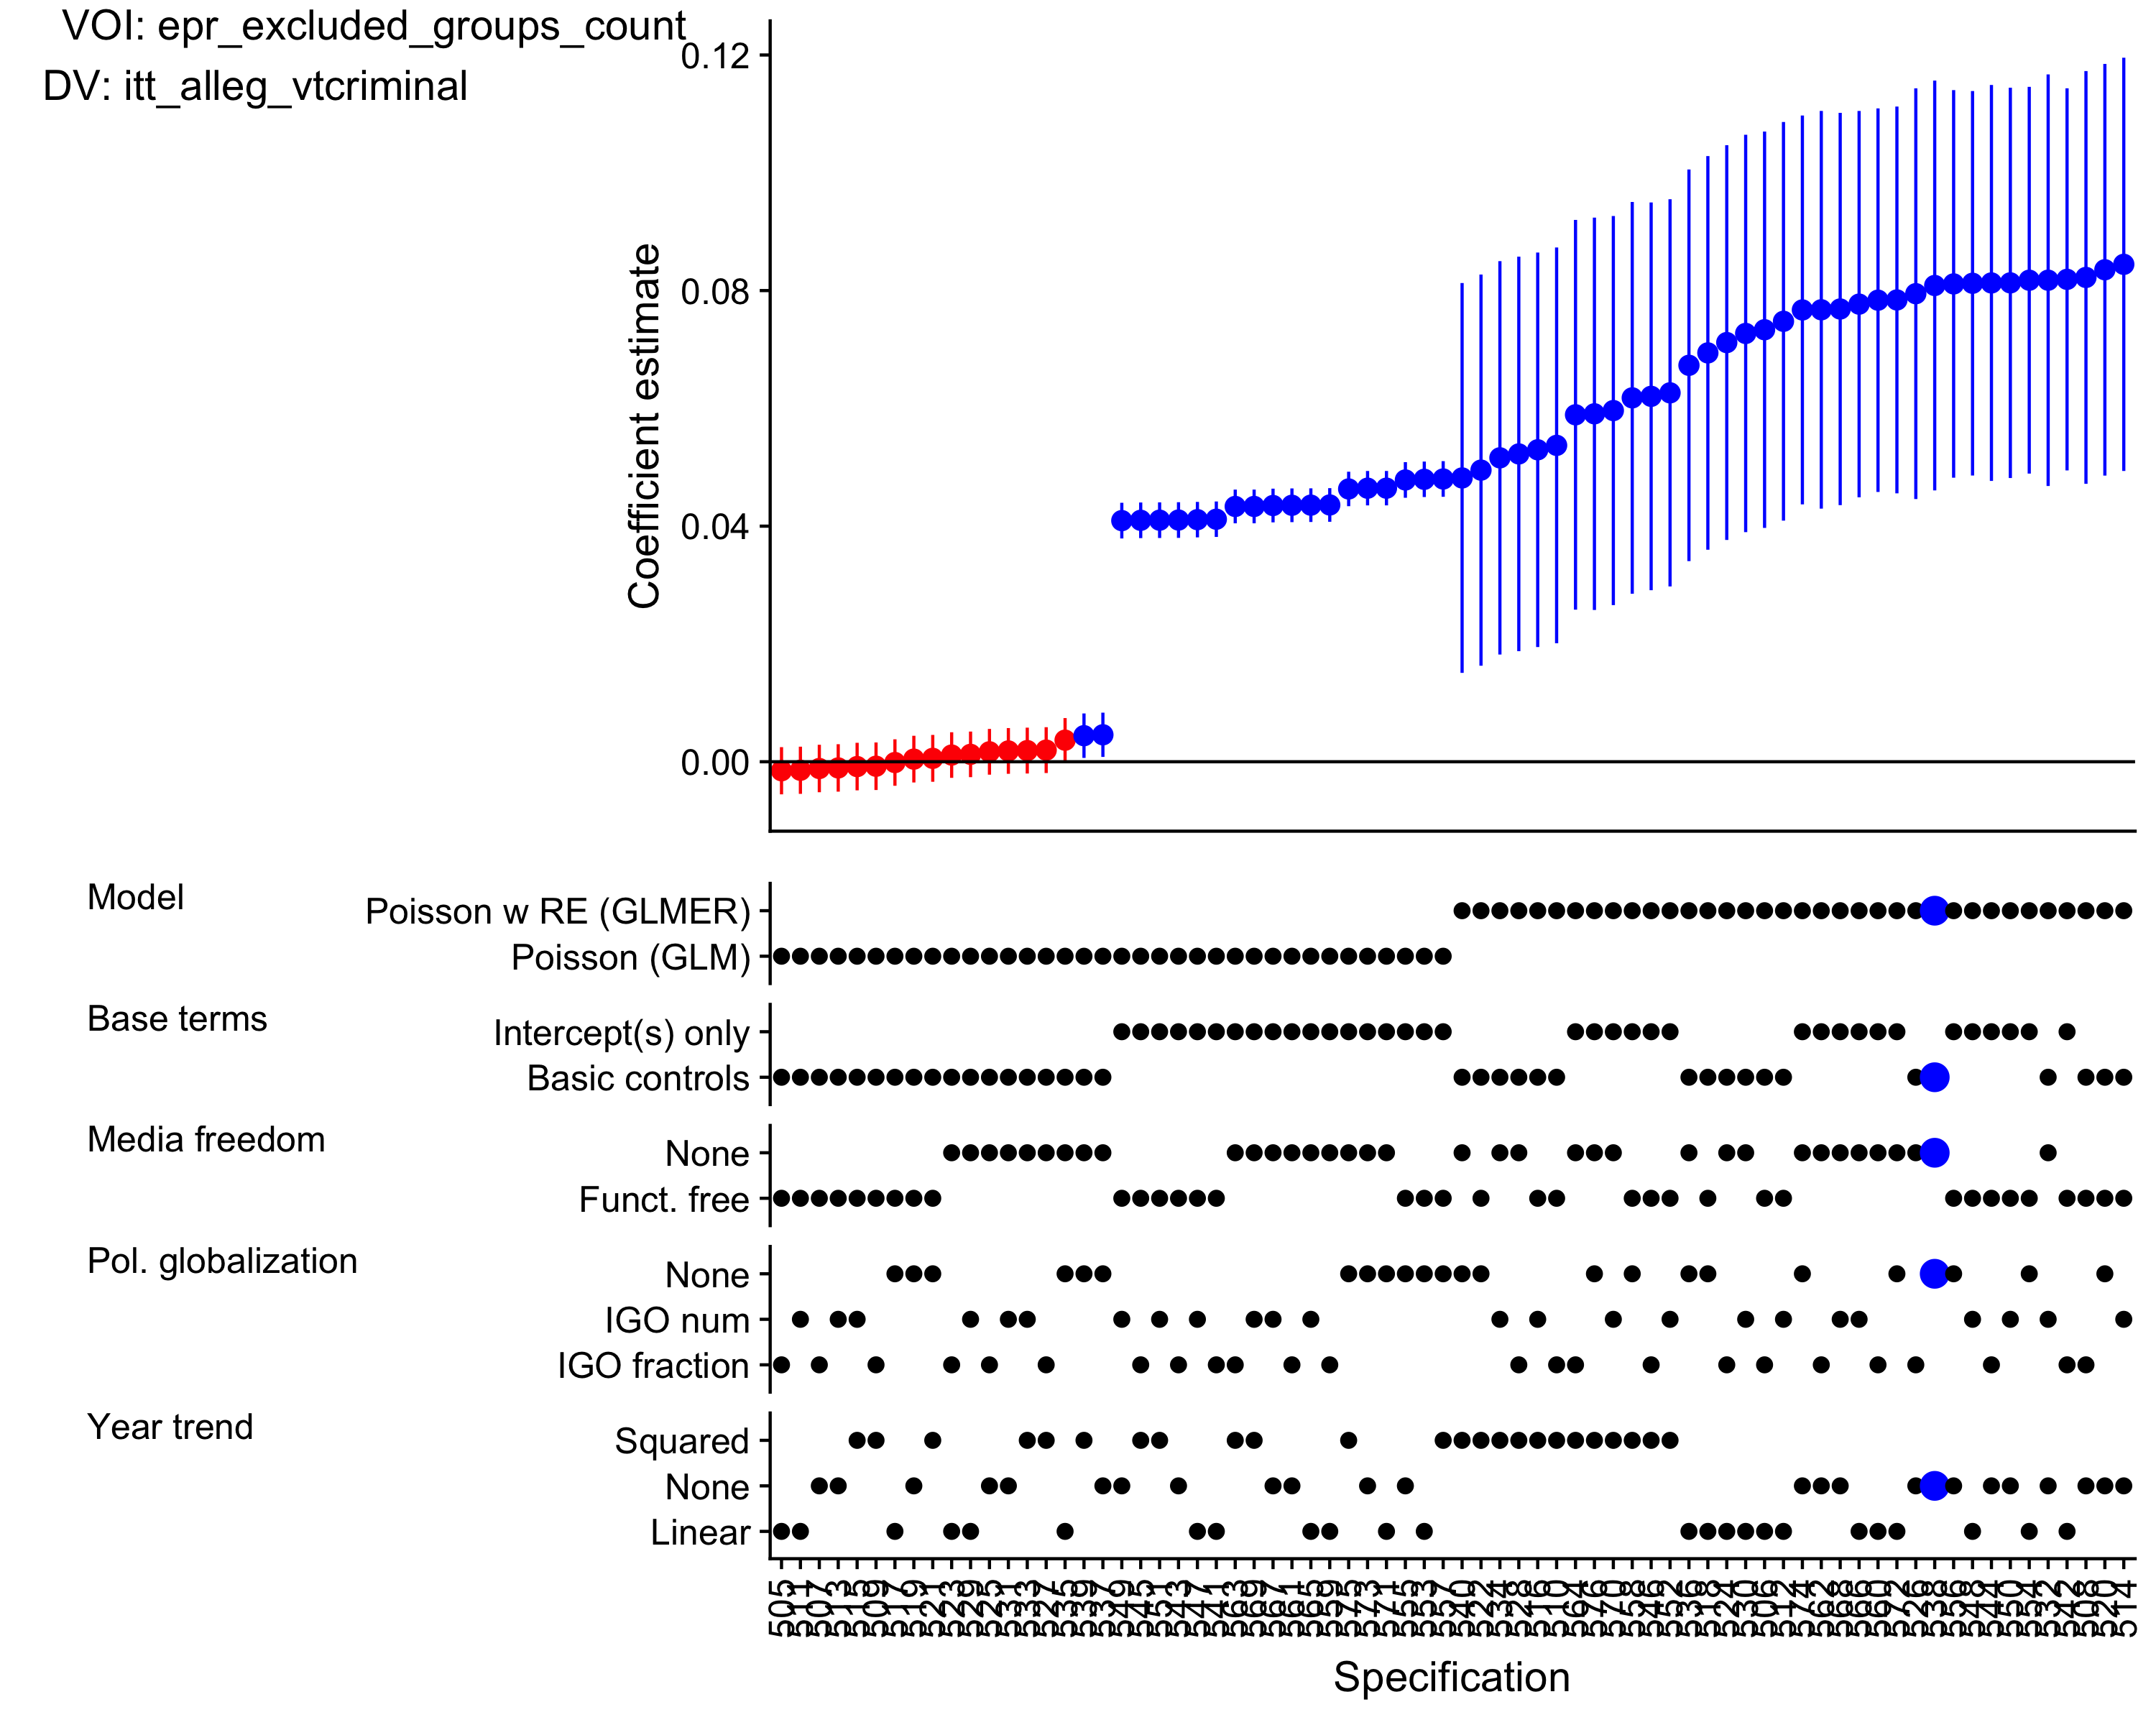
\includegraphics[height=4in]{../output/figures-robustness/specplot-epr_excluded_groups_count-itt_alleg_vtcriminal.png}

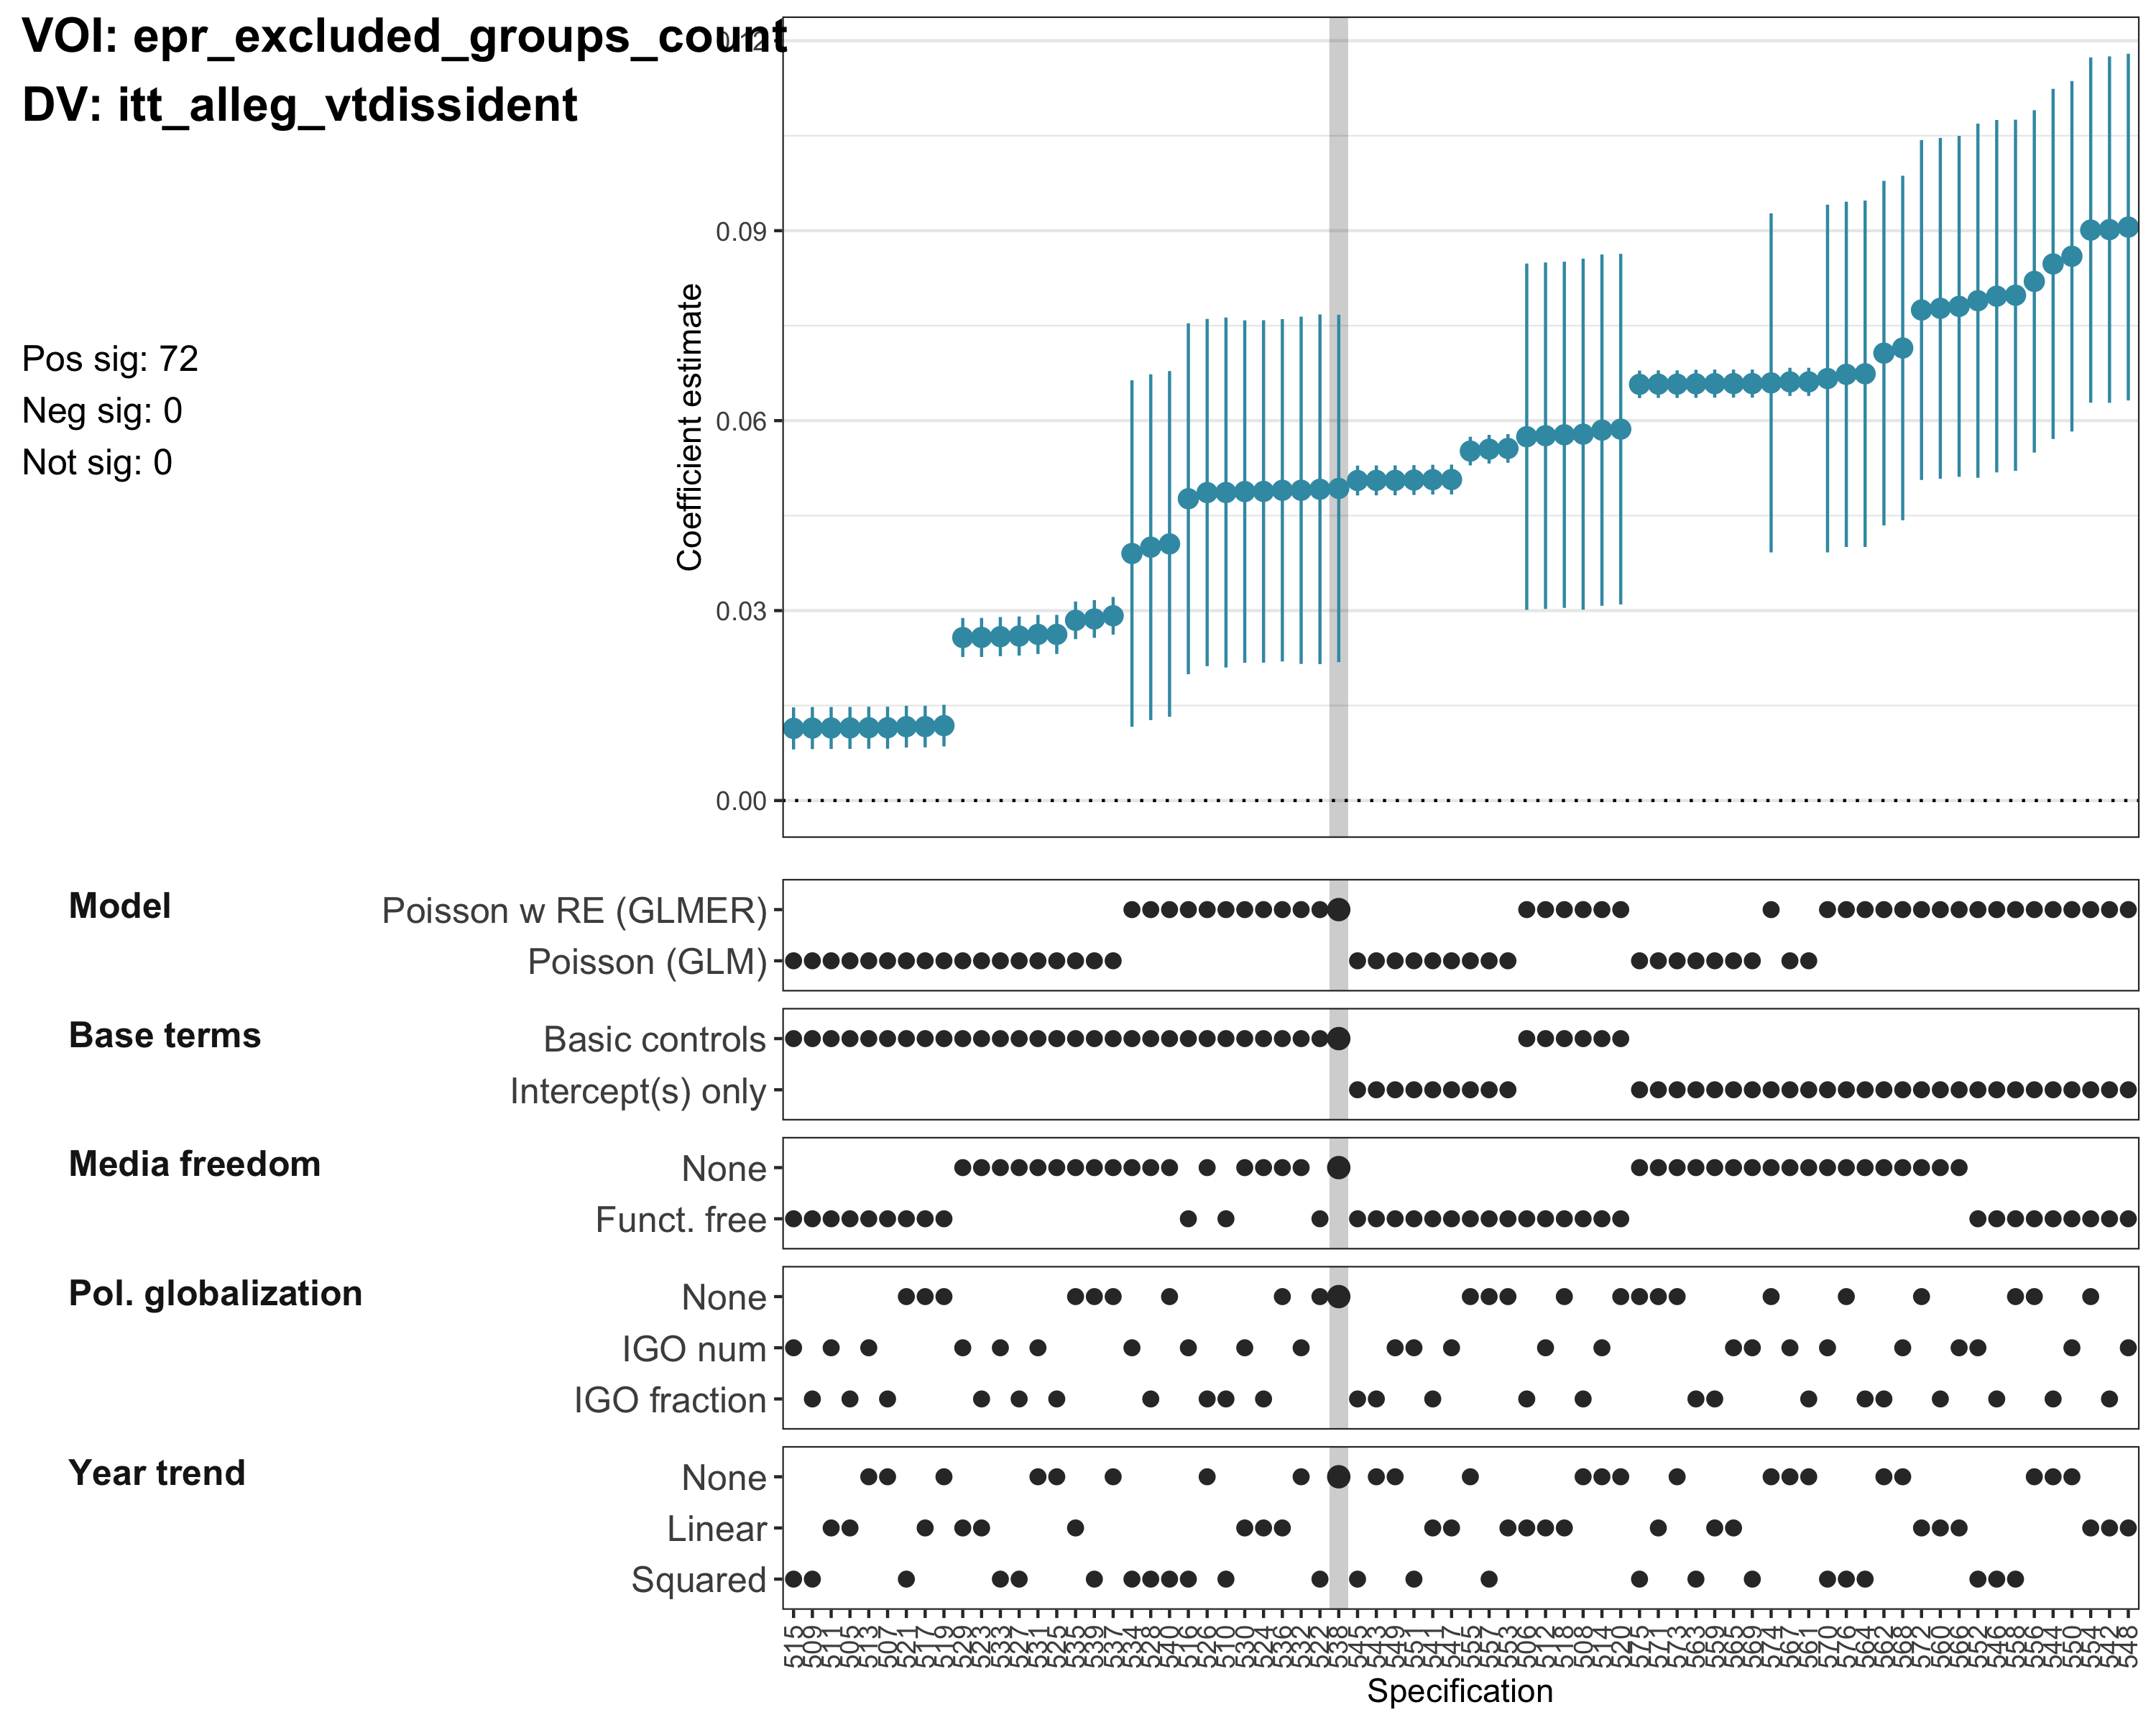
\includegraphics[height=4in]{../output/figures-robustness/specplot-epr_excluded_groups_count-itt_alleg_vtdissident.png}

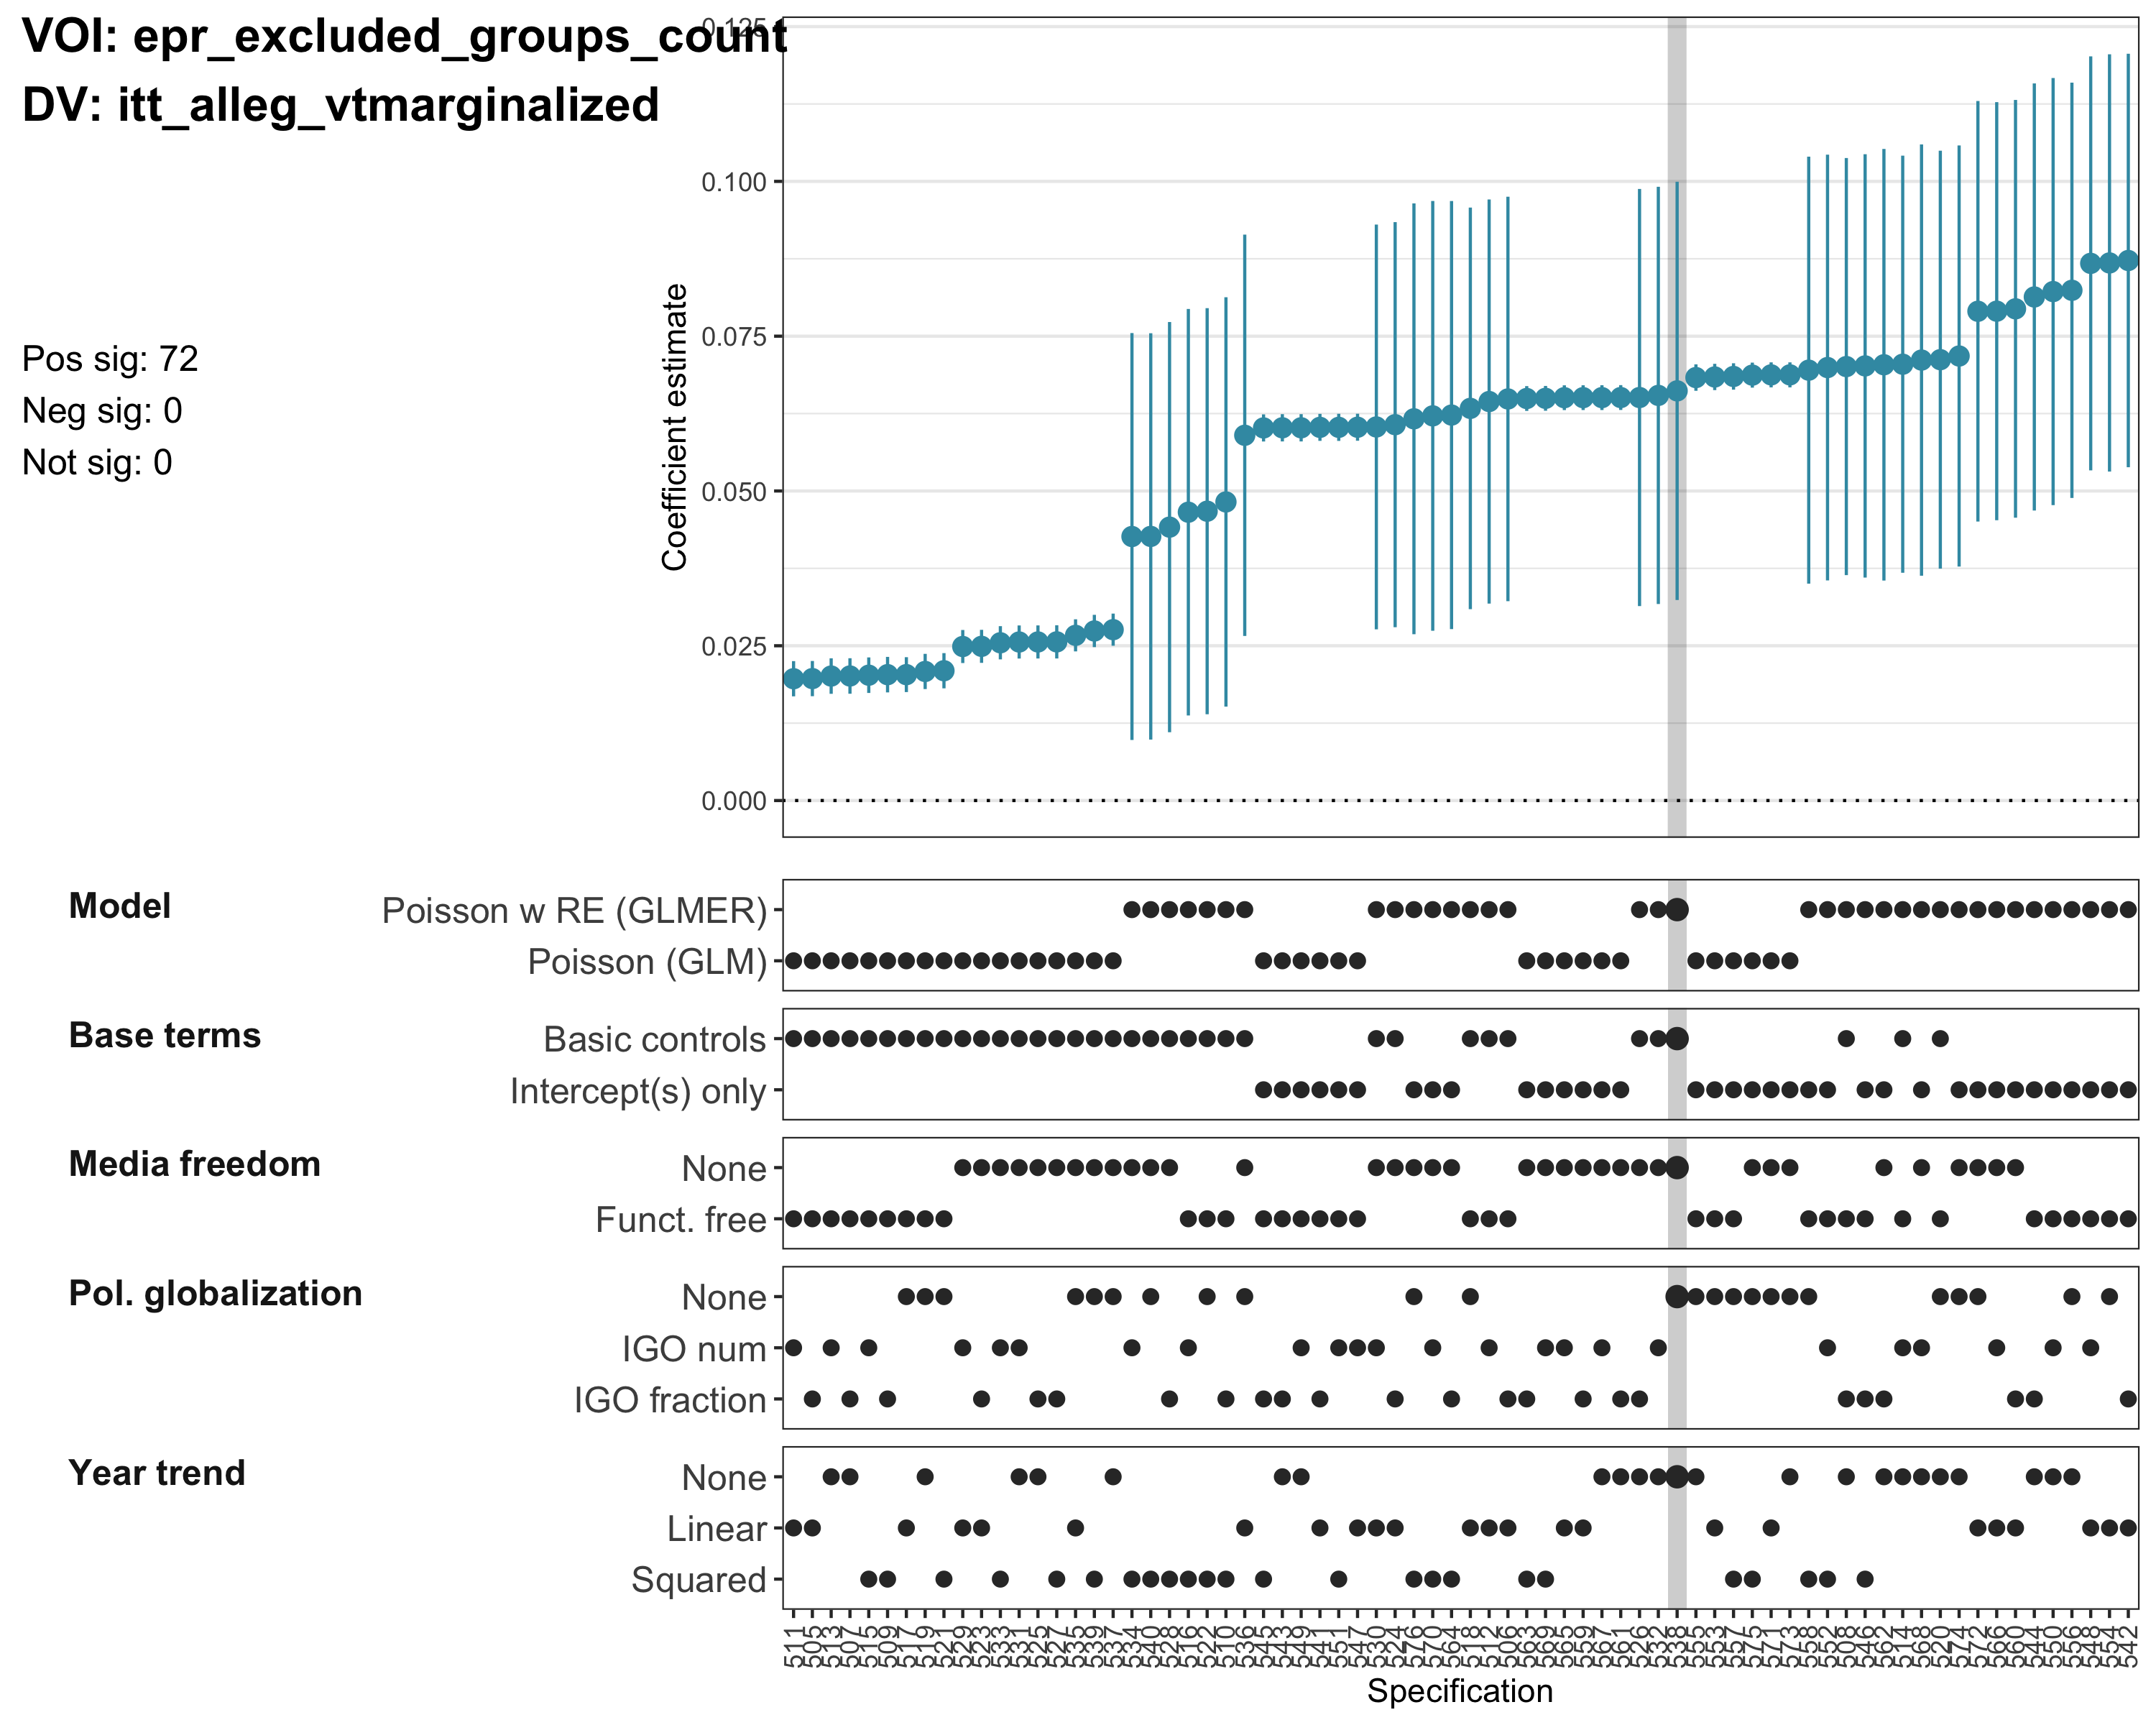
\includegraphics[height=4in]{../output/figures-robustness/specplot-epr_excluded_groups_count-itt_alleg_vtmarginalized.png}

\hypertarget{voi-v2clacjust}{%
\subsection{VOI: v2clacjust}\label{voi-v2clacjust}}

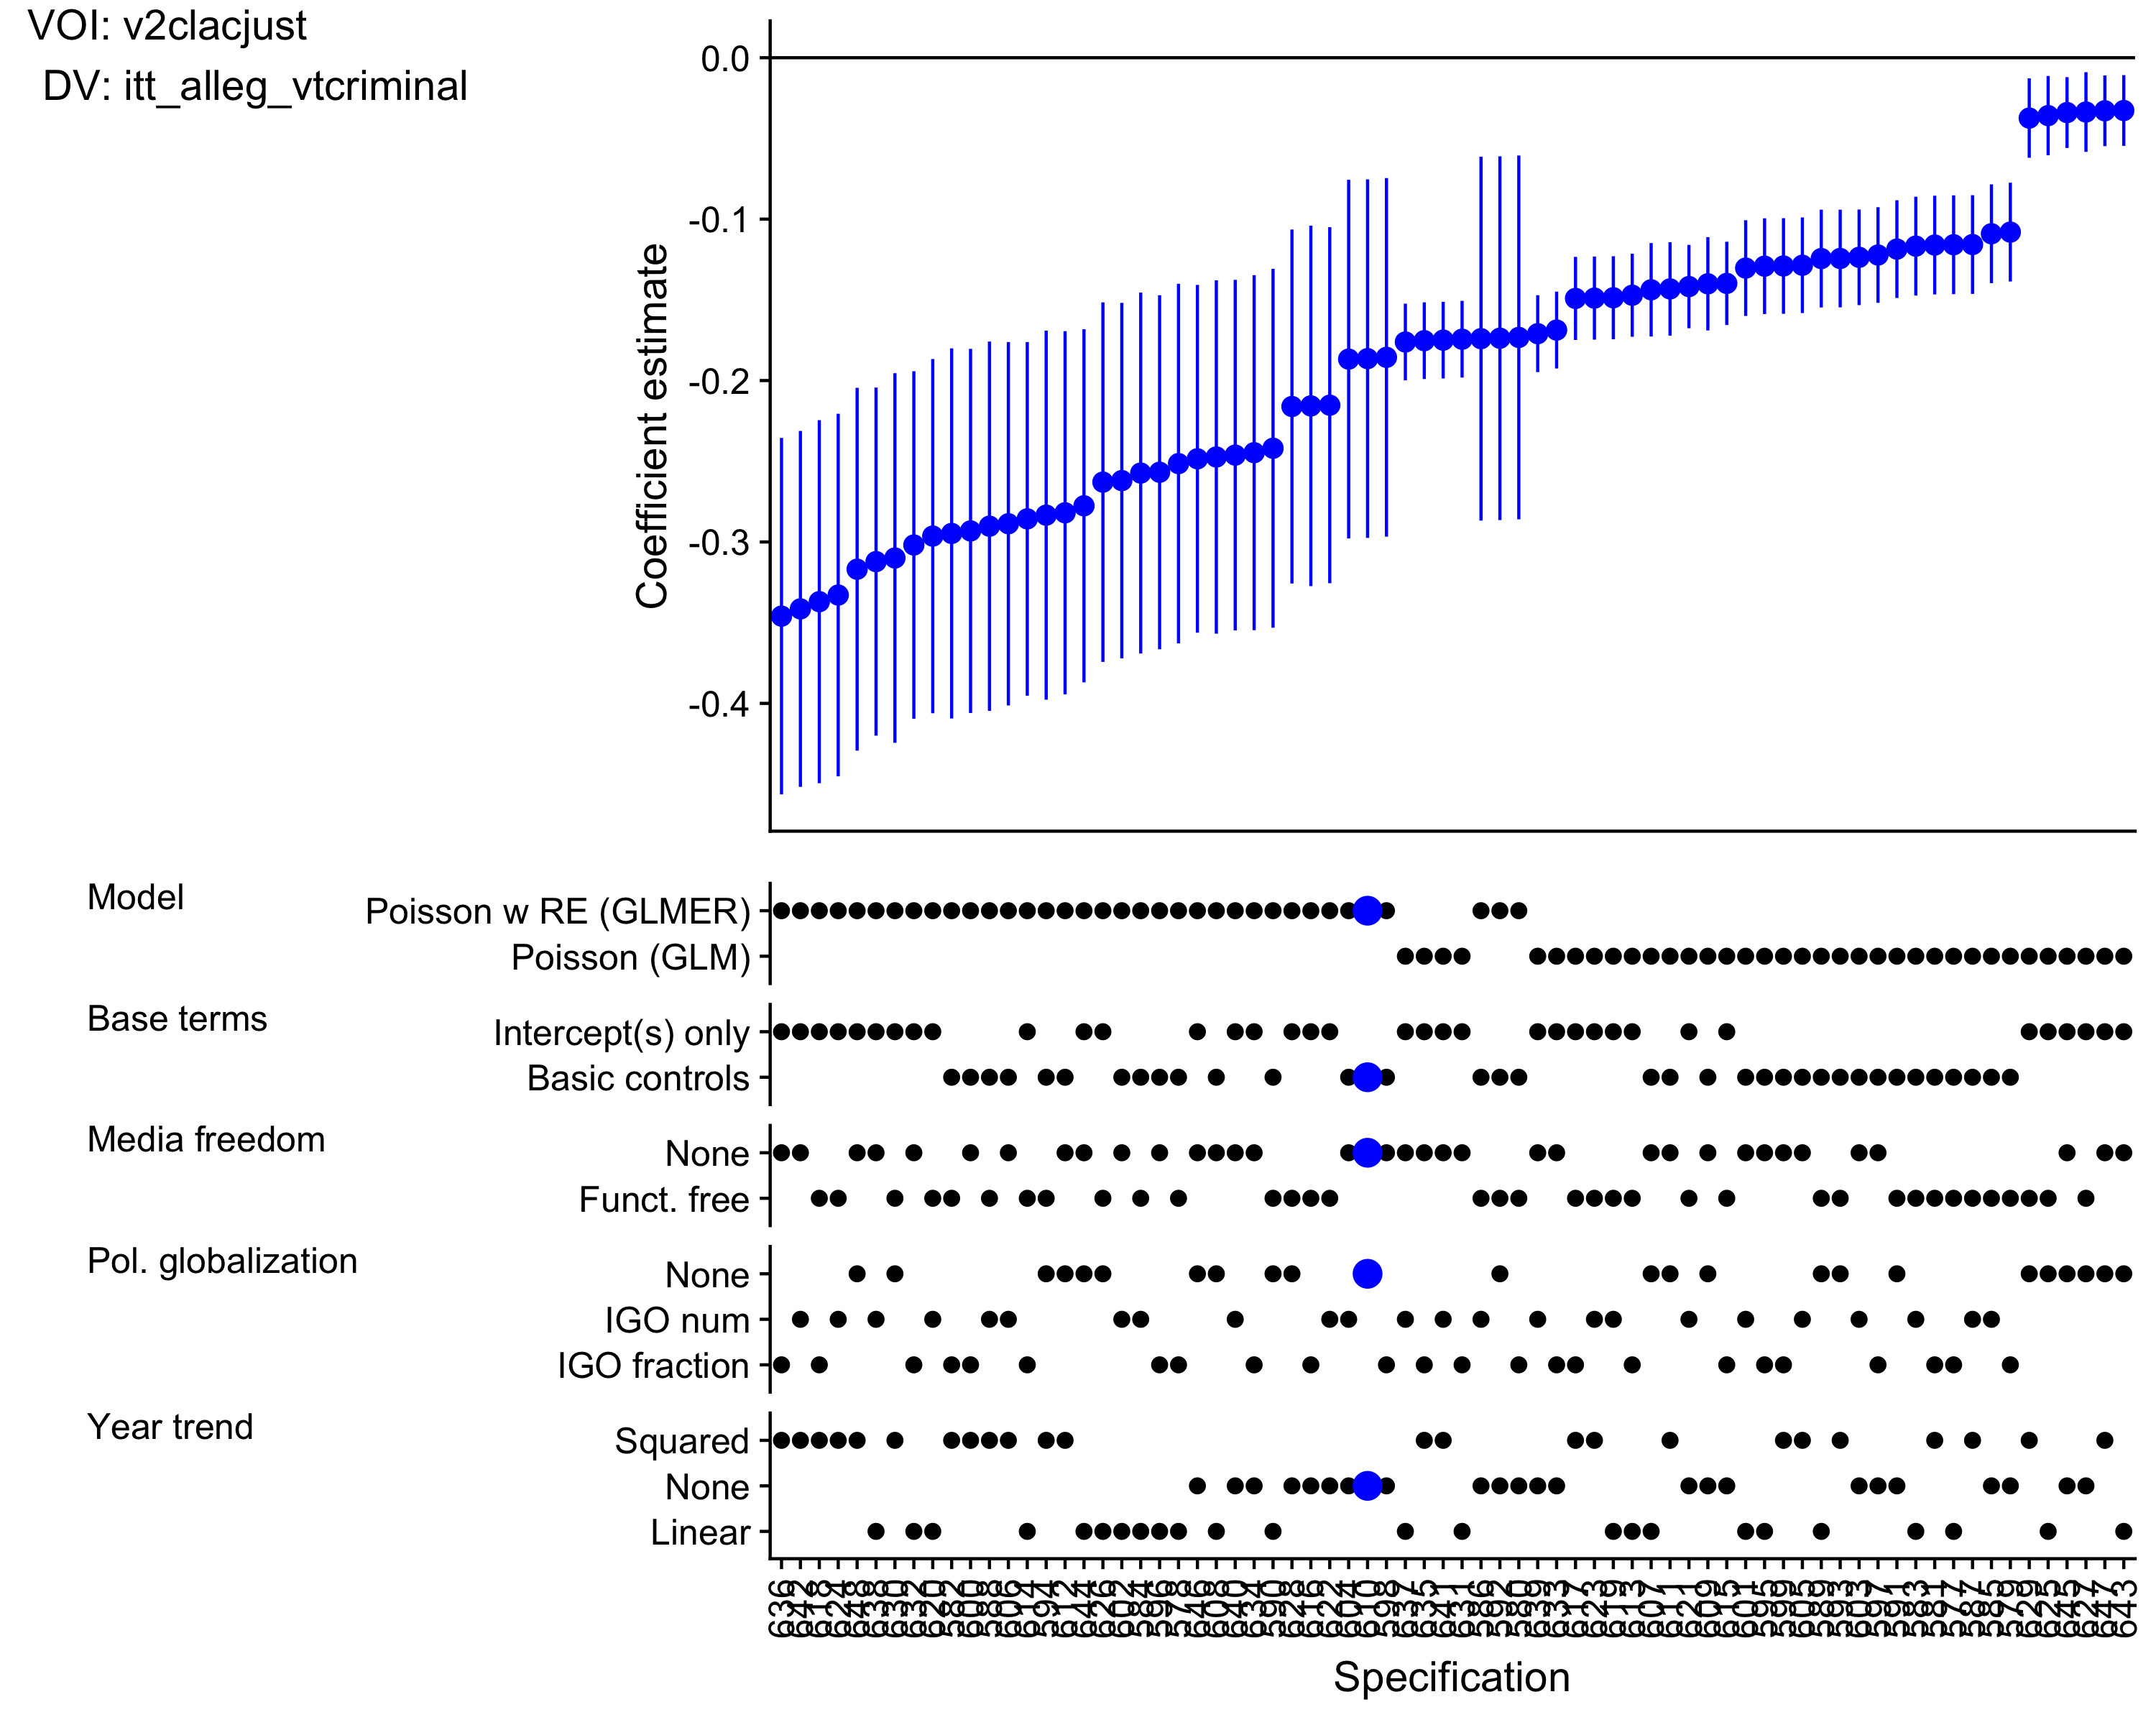
\includegraphics[height=4in]{../output/figures-robustness/specplot-v2clacjust-itt_alleg_vtcriminal.png}

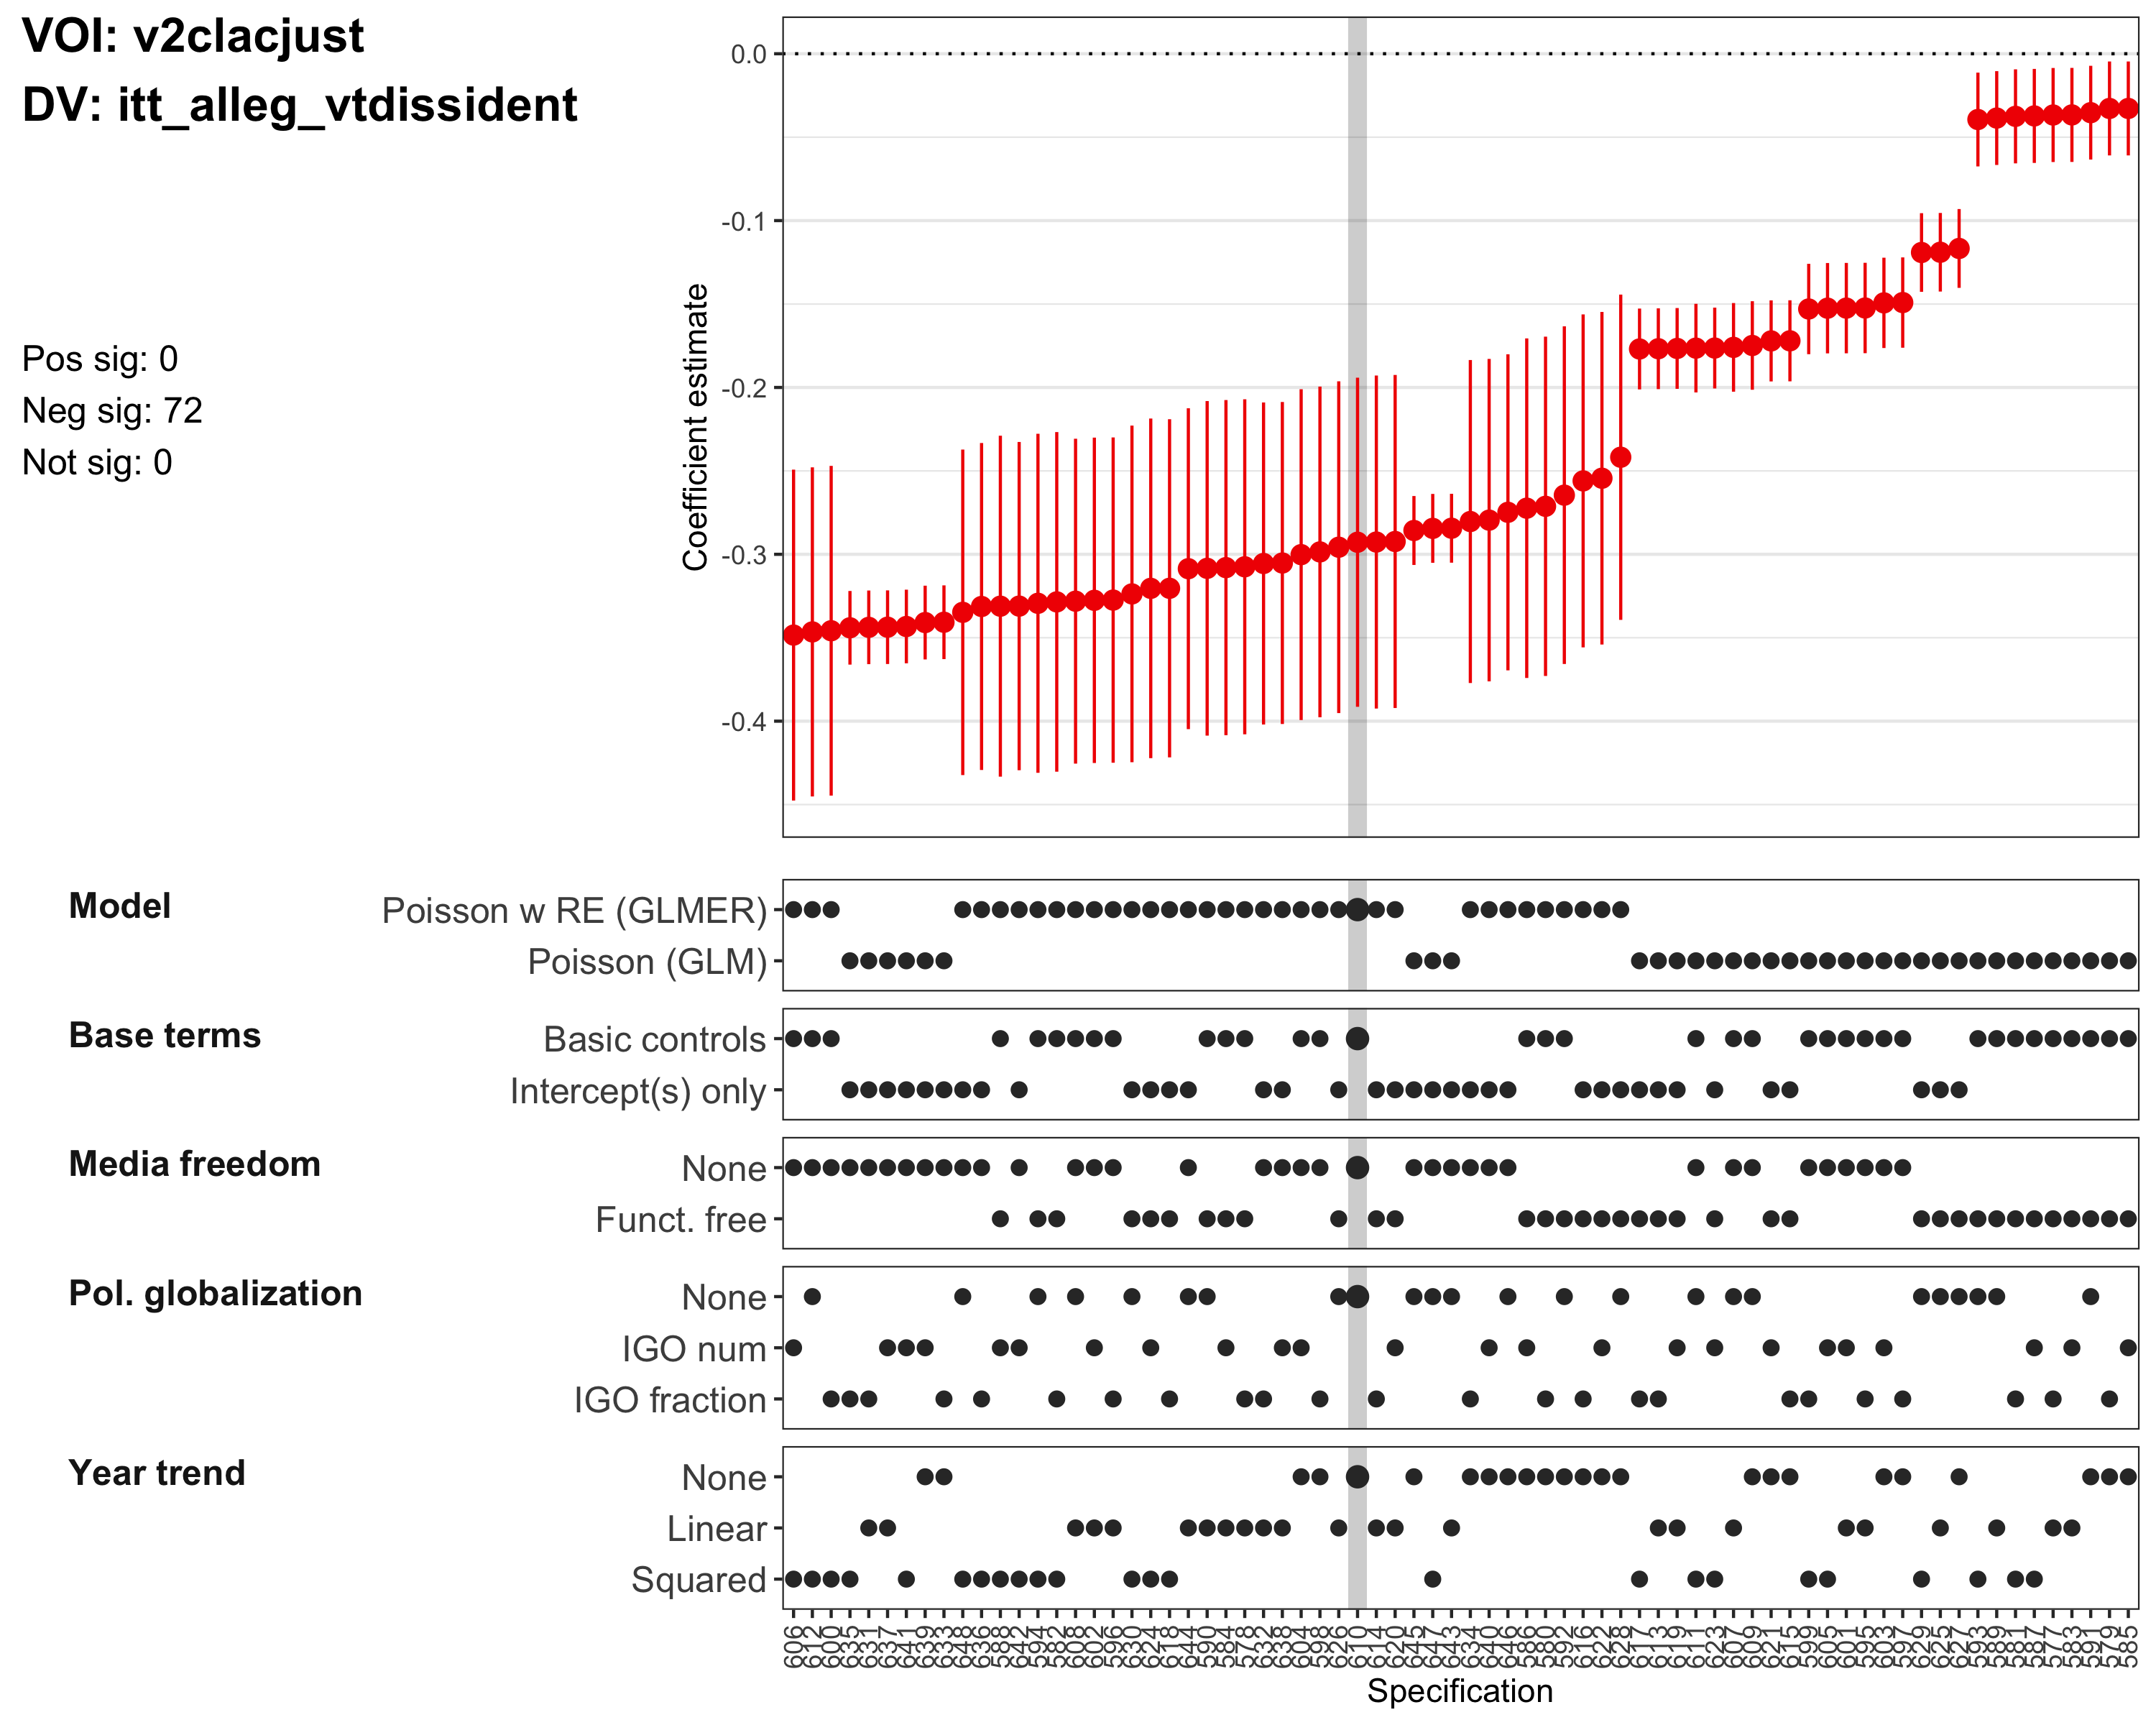
\includegraphics[height=4in]{../output/figures-robustness/specplot-v2clacjust-itt_alleg_vtdissident.png}

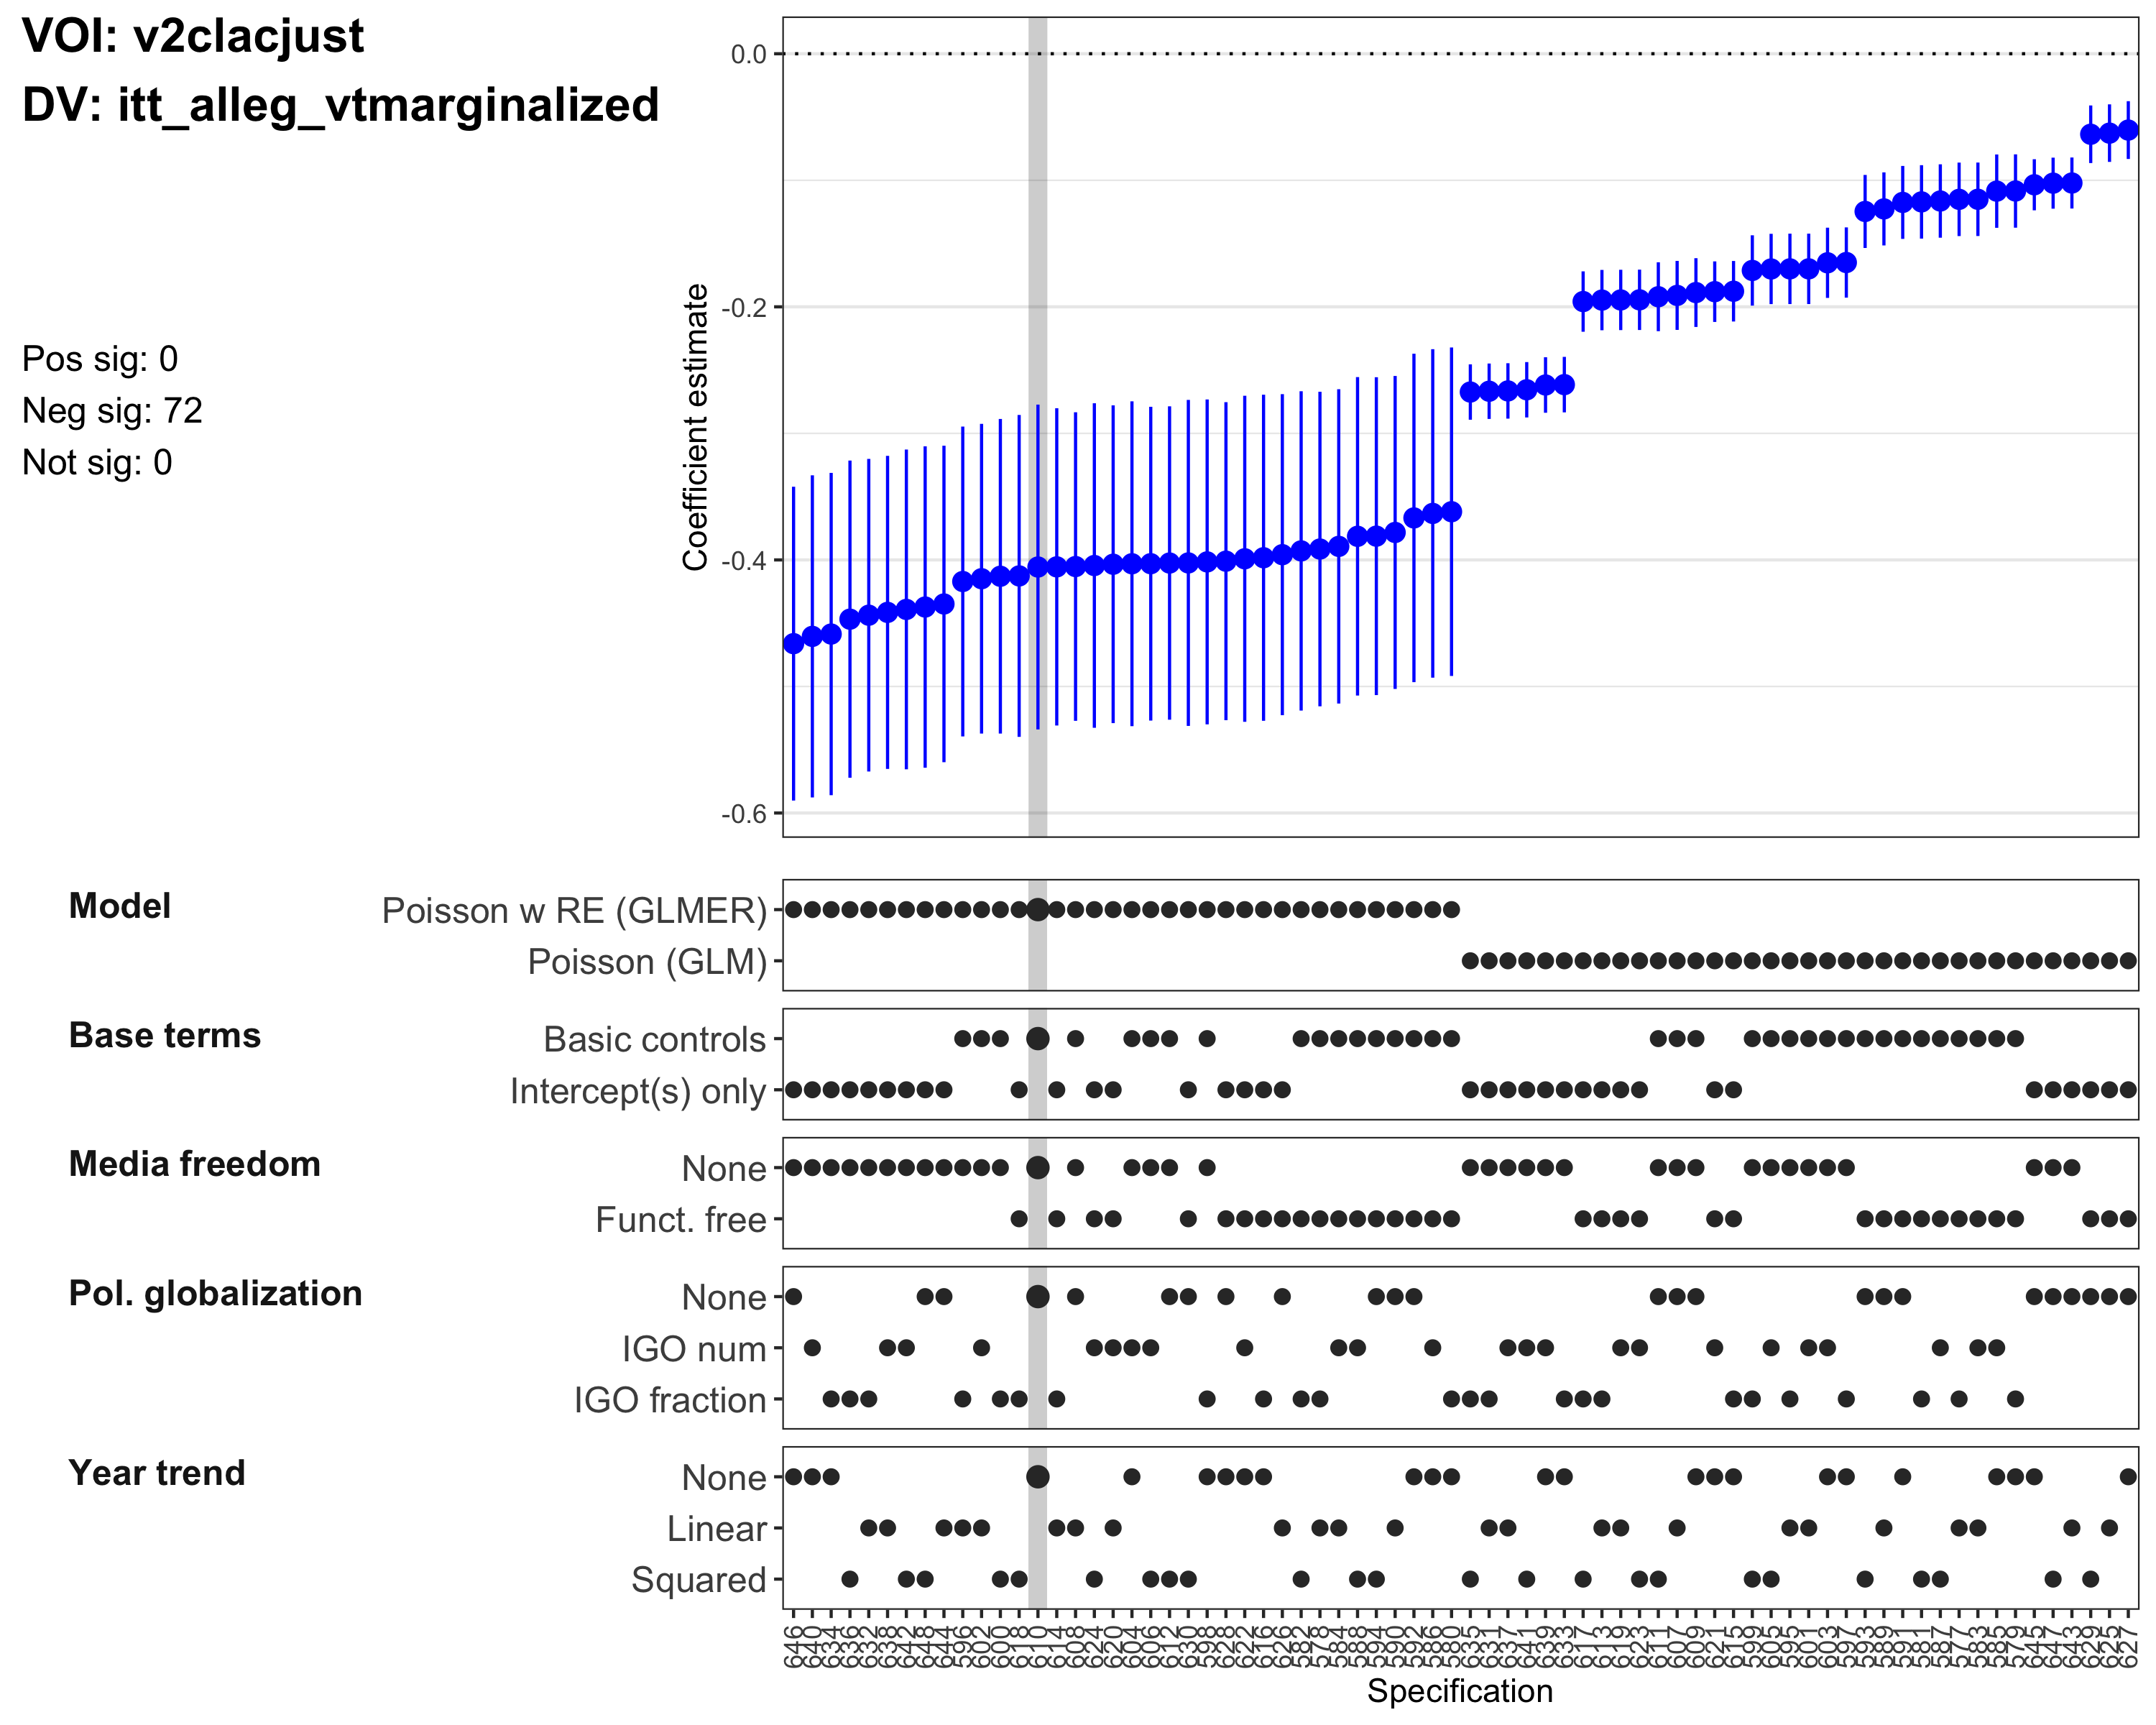
\includegraphics[height=4in]{../output/figures-robustness/specplot-v2clacjust-itt_alleg_vtmarginalized.png}

\hypertarget{voi-v2clsocgrp}{%
\subsection{VOI: v2clsocgrp}\label{voi-v2clsocgrp}}

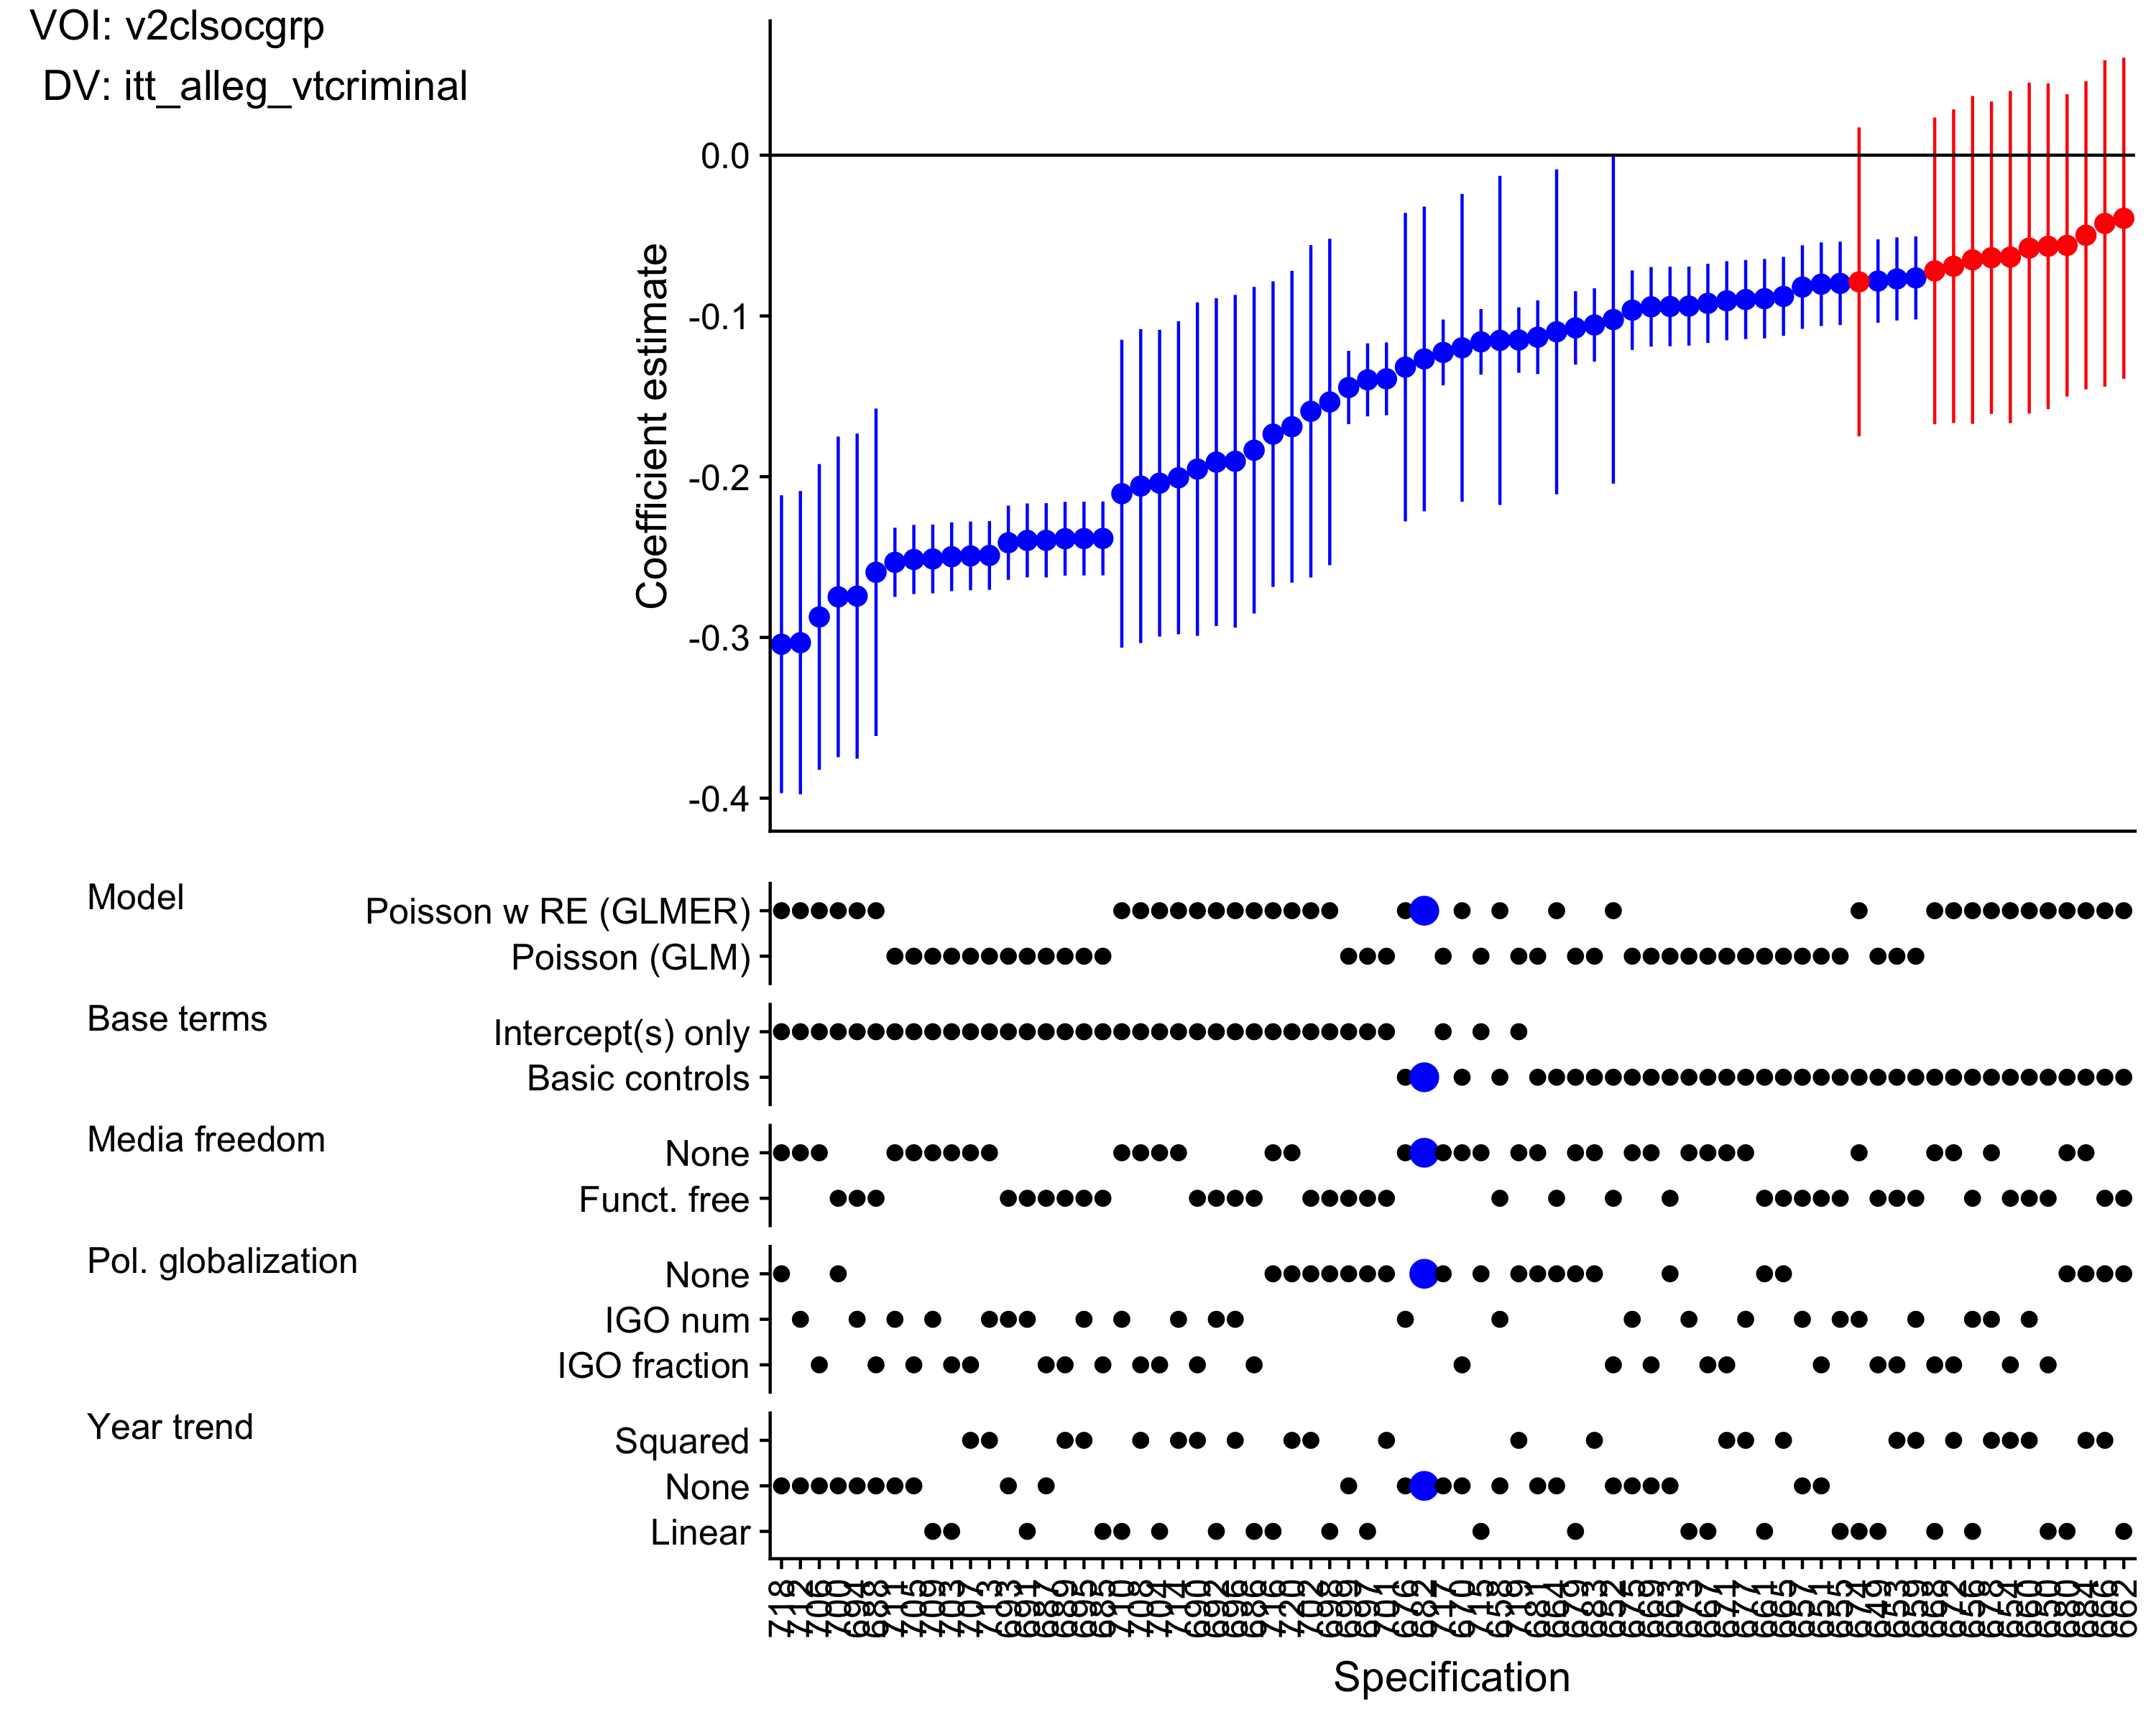
\includegraphics[height=4in]{../output/figures-robustness/specplot-v2clsocgrp-itt_alleg_vtcriminal.png}

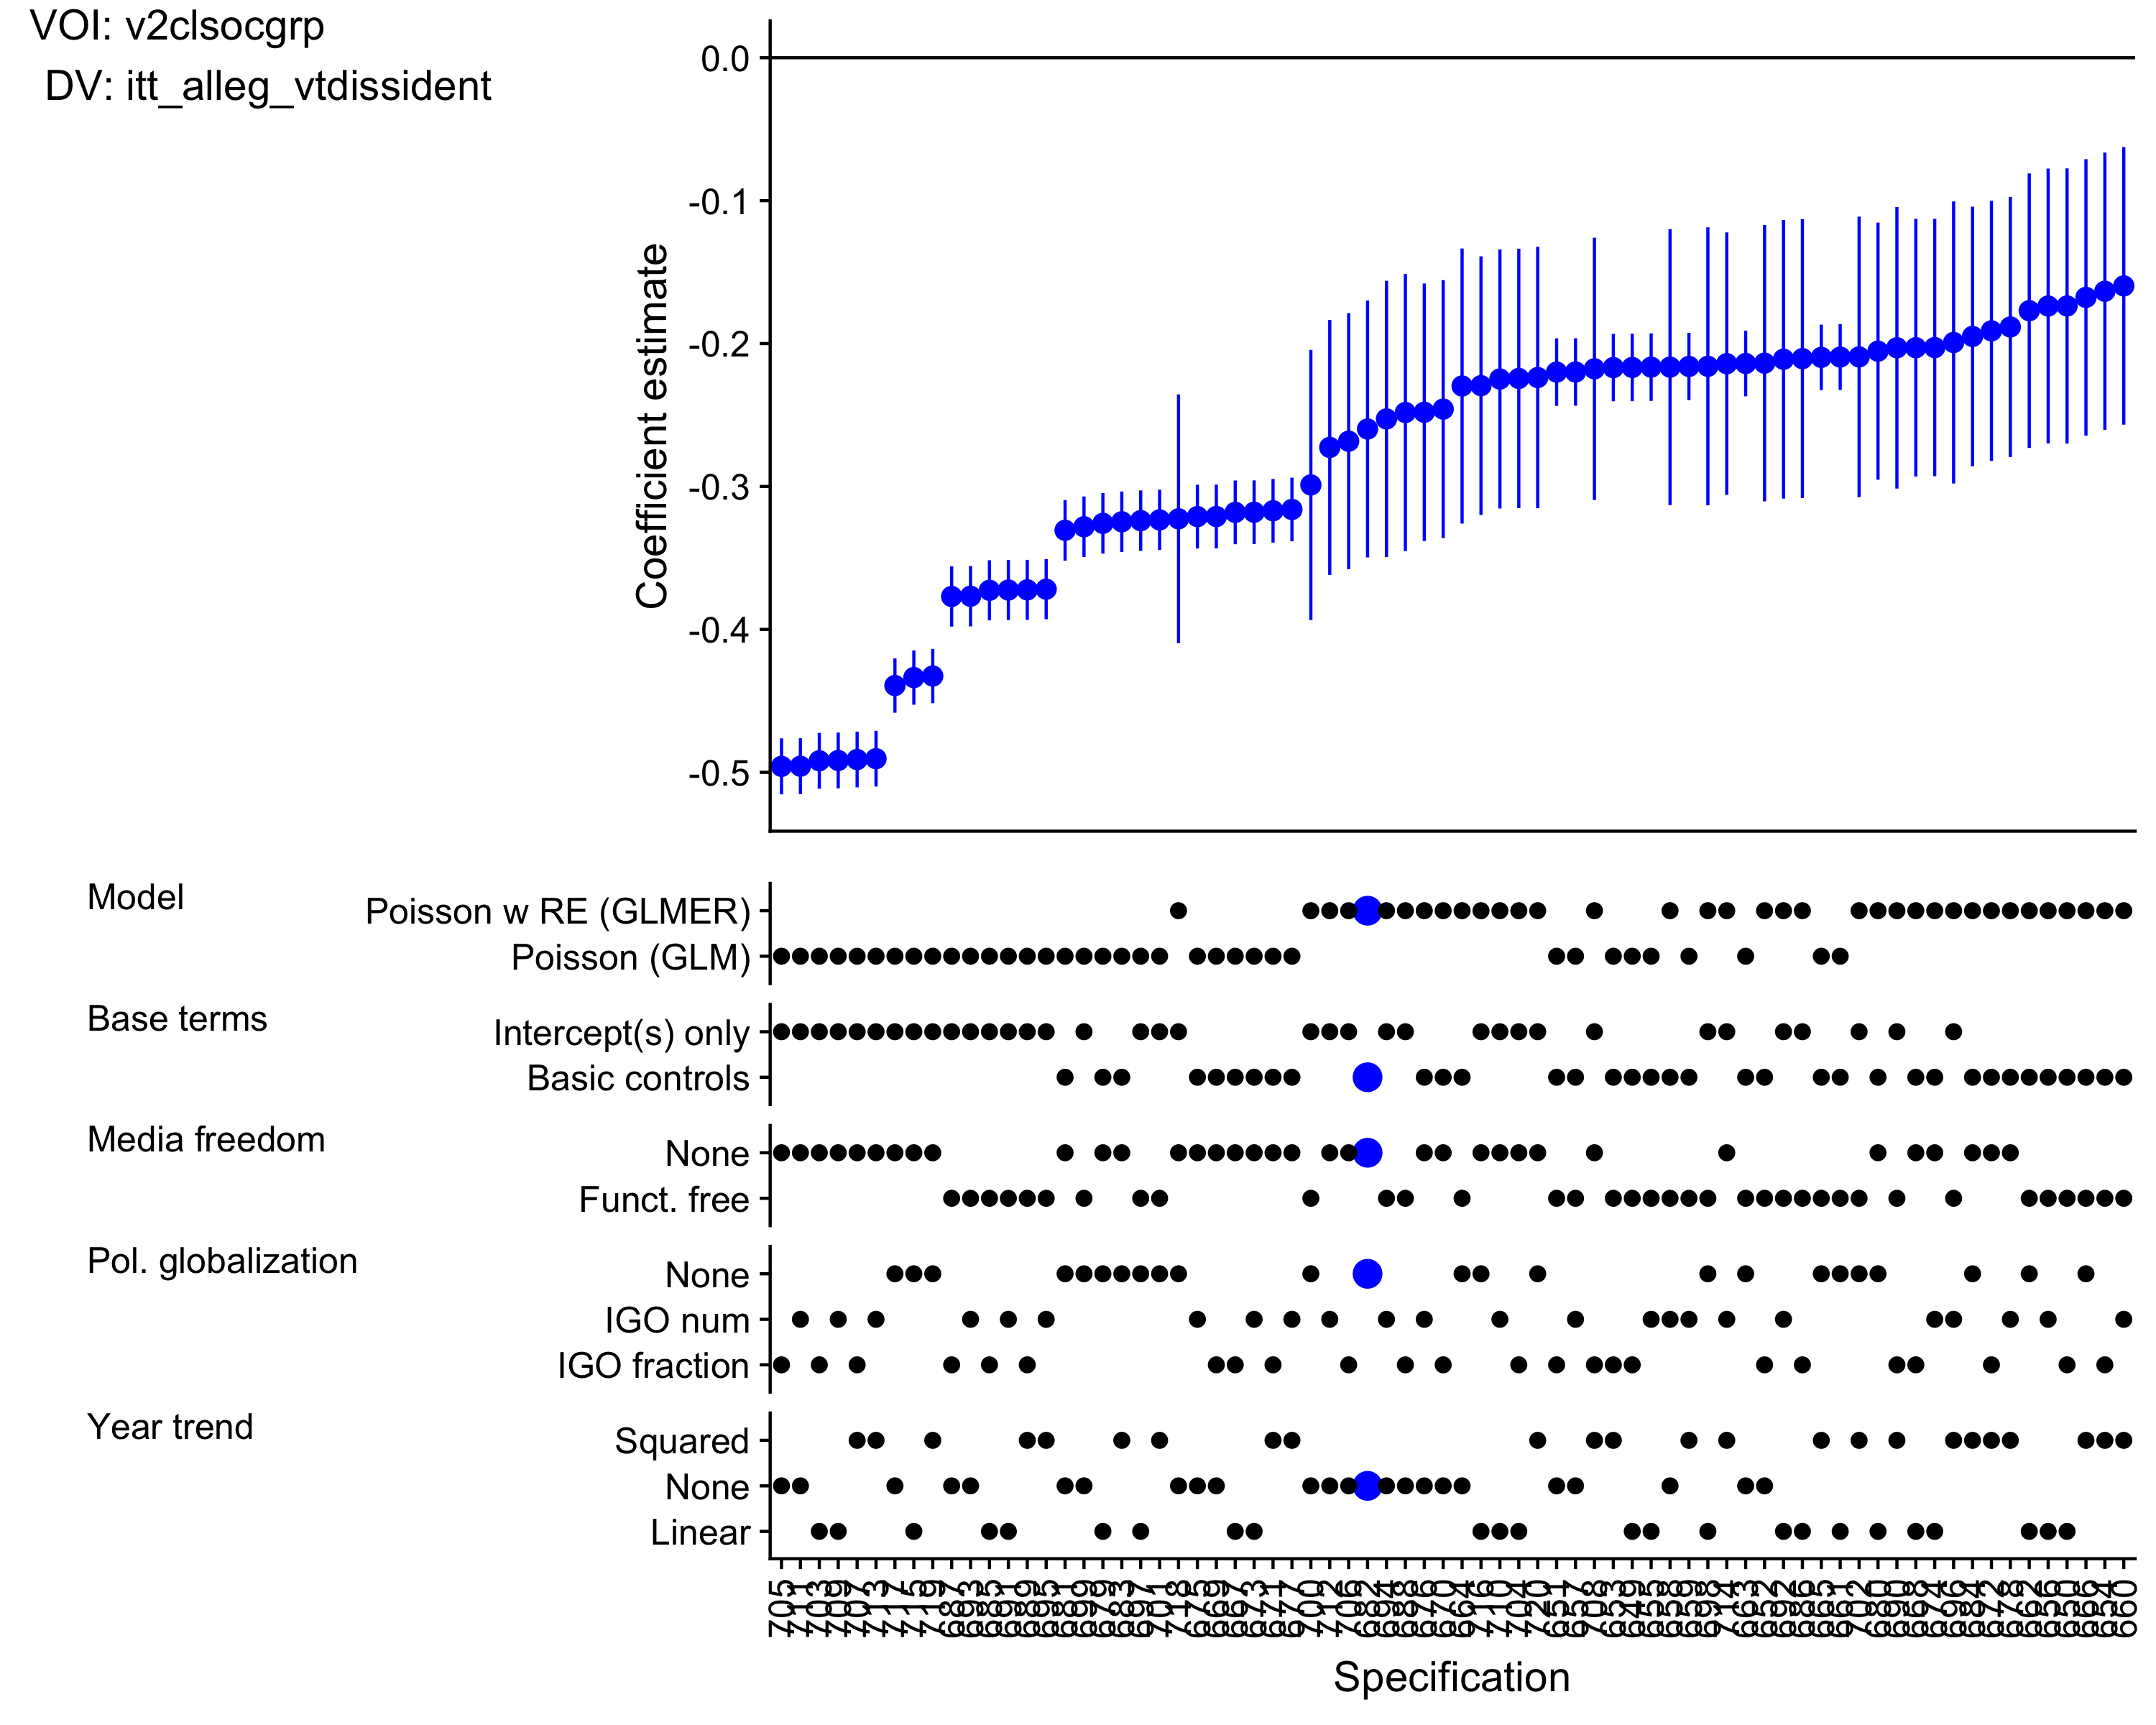
\includegraphics[height=4in]{../output/figures-robustness/specplot-v2clsocgrp-itt_alleg_vtdissident.png}

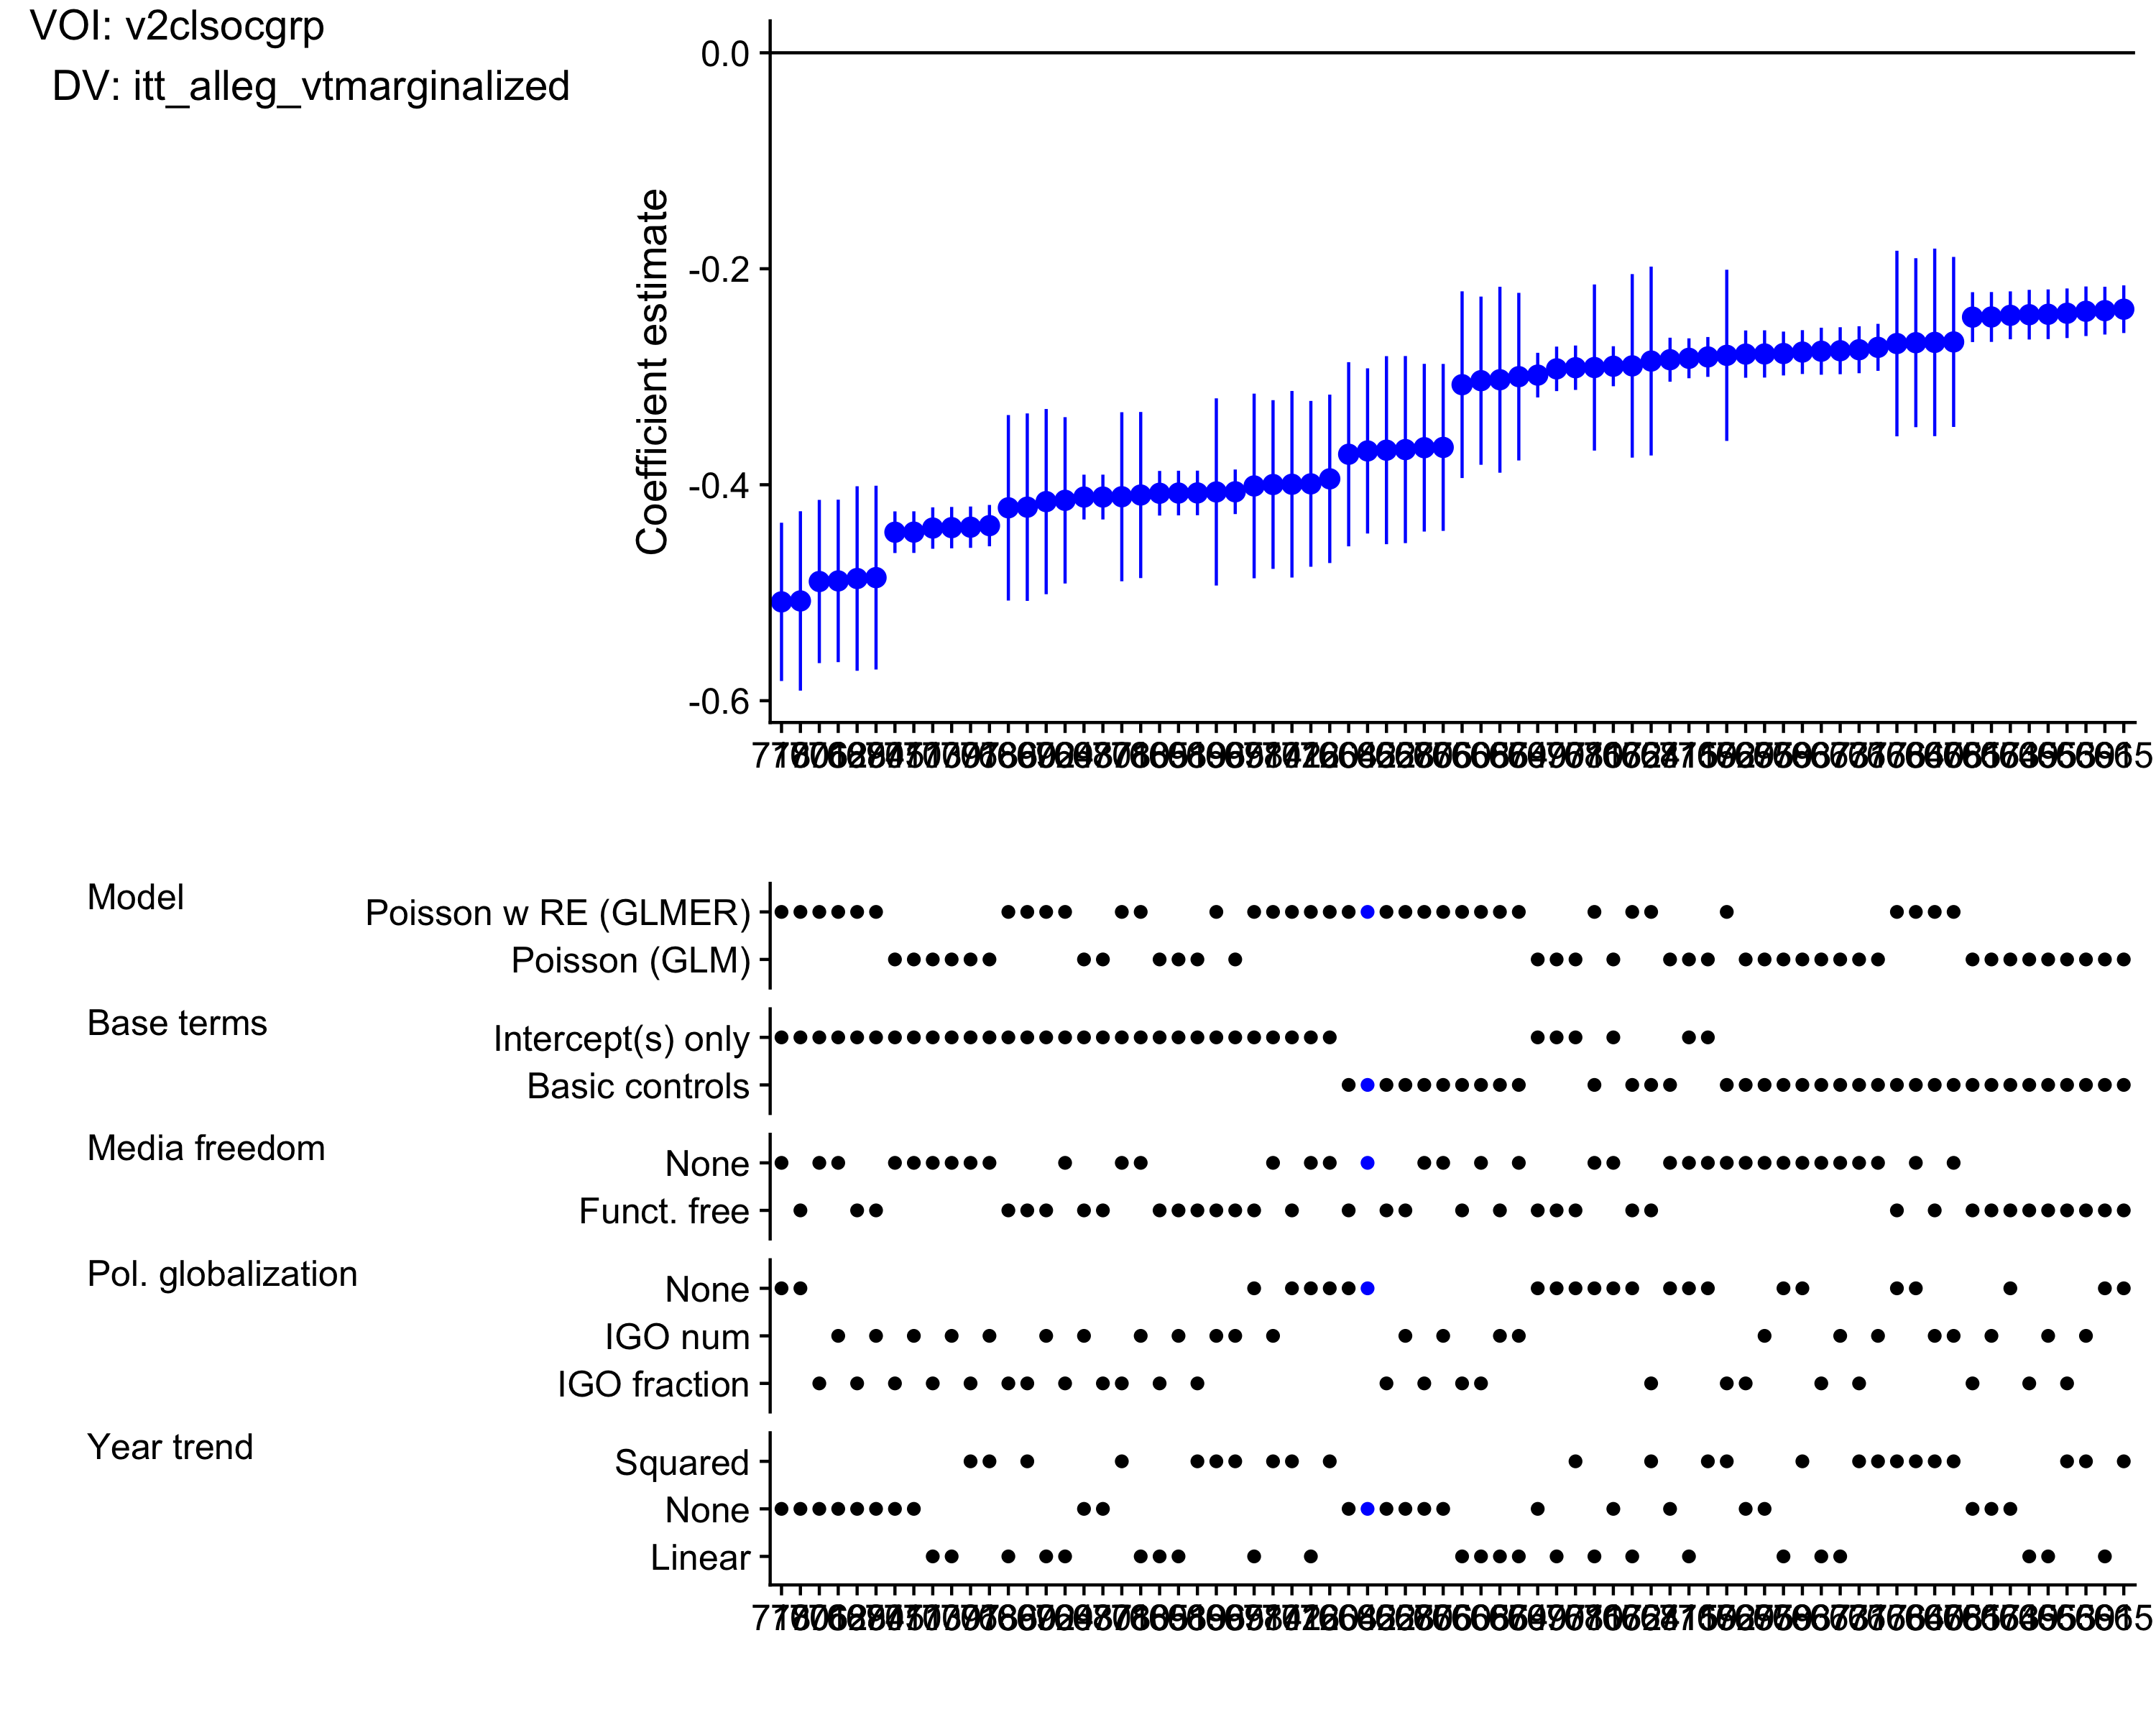
\includegraphics[height=4in]{../output/figures-robustness/specplot-v2clsocgrp-itt_alleg_vtmarginalized.png}

\hypertarget{voi-v2pepwrses}{%
\subsection{VOI: v2pepwrses}\label{voi-v2pepwrses}}

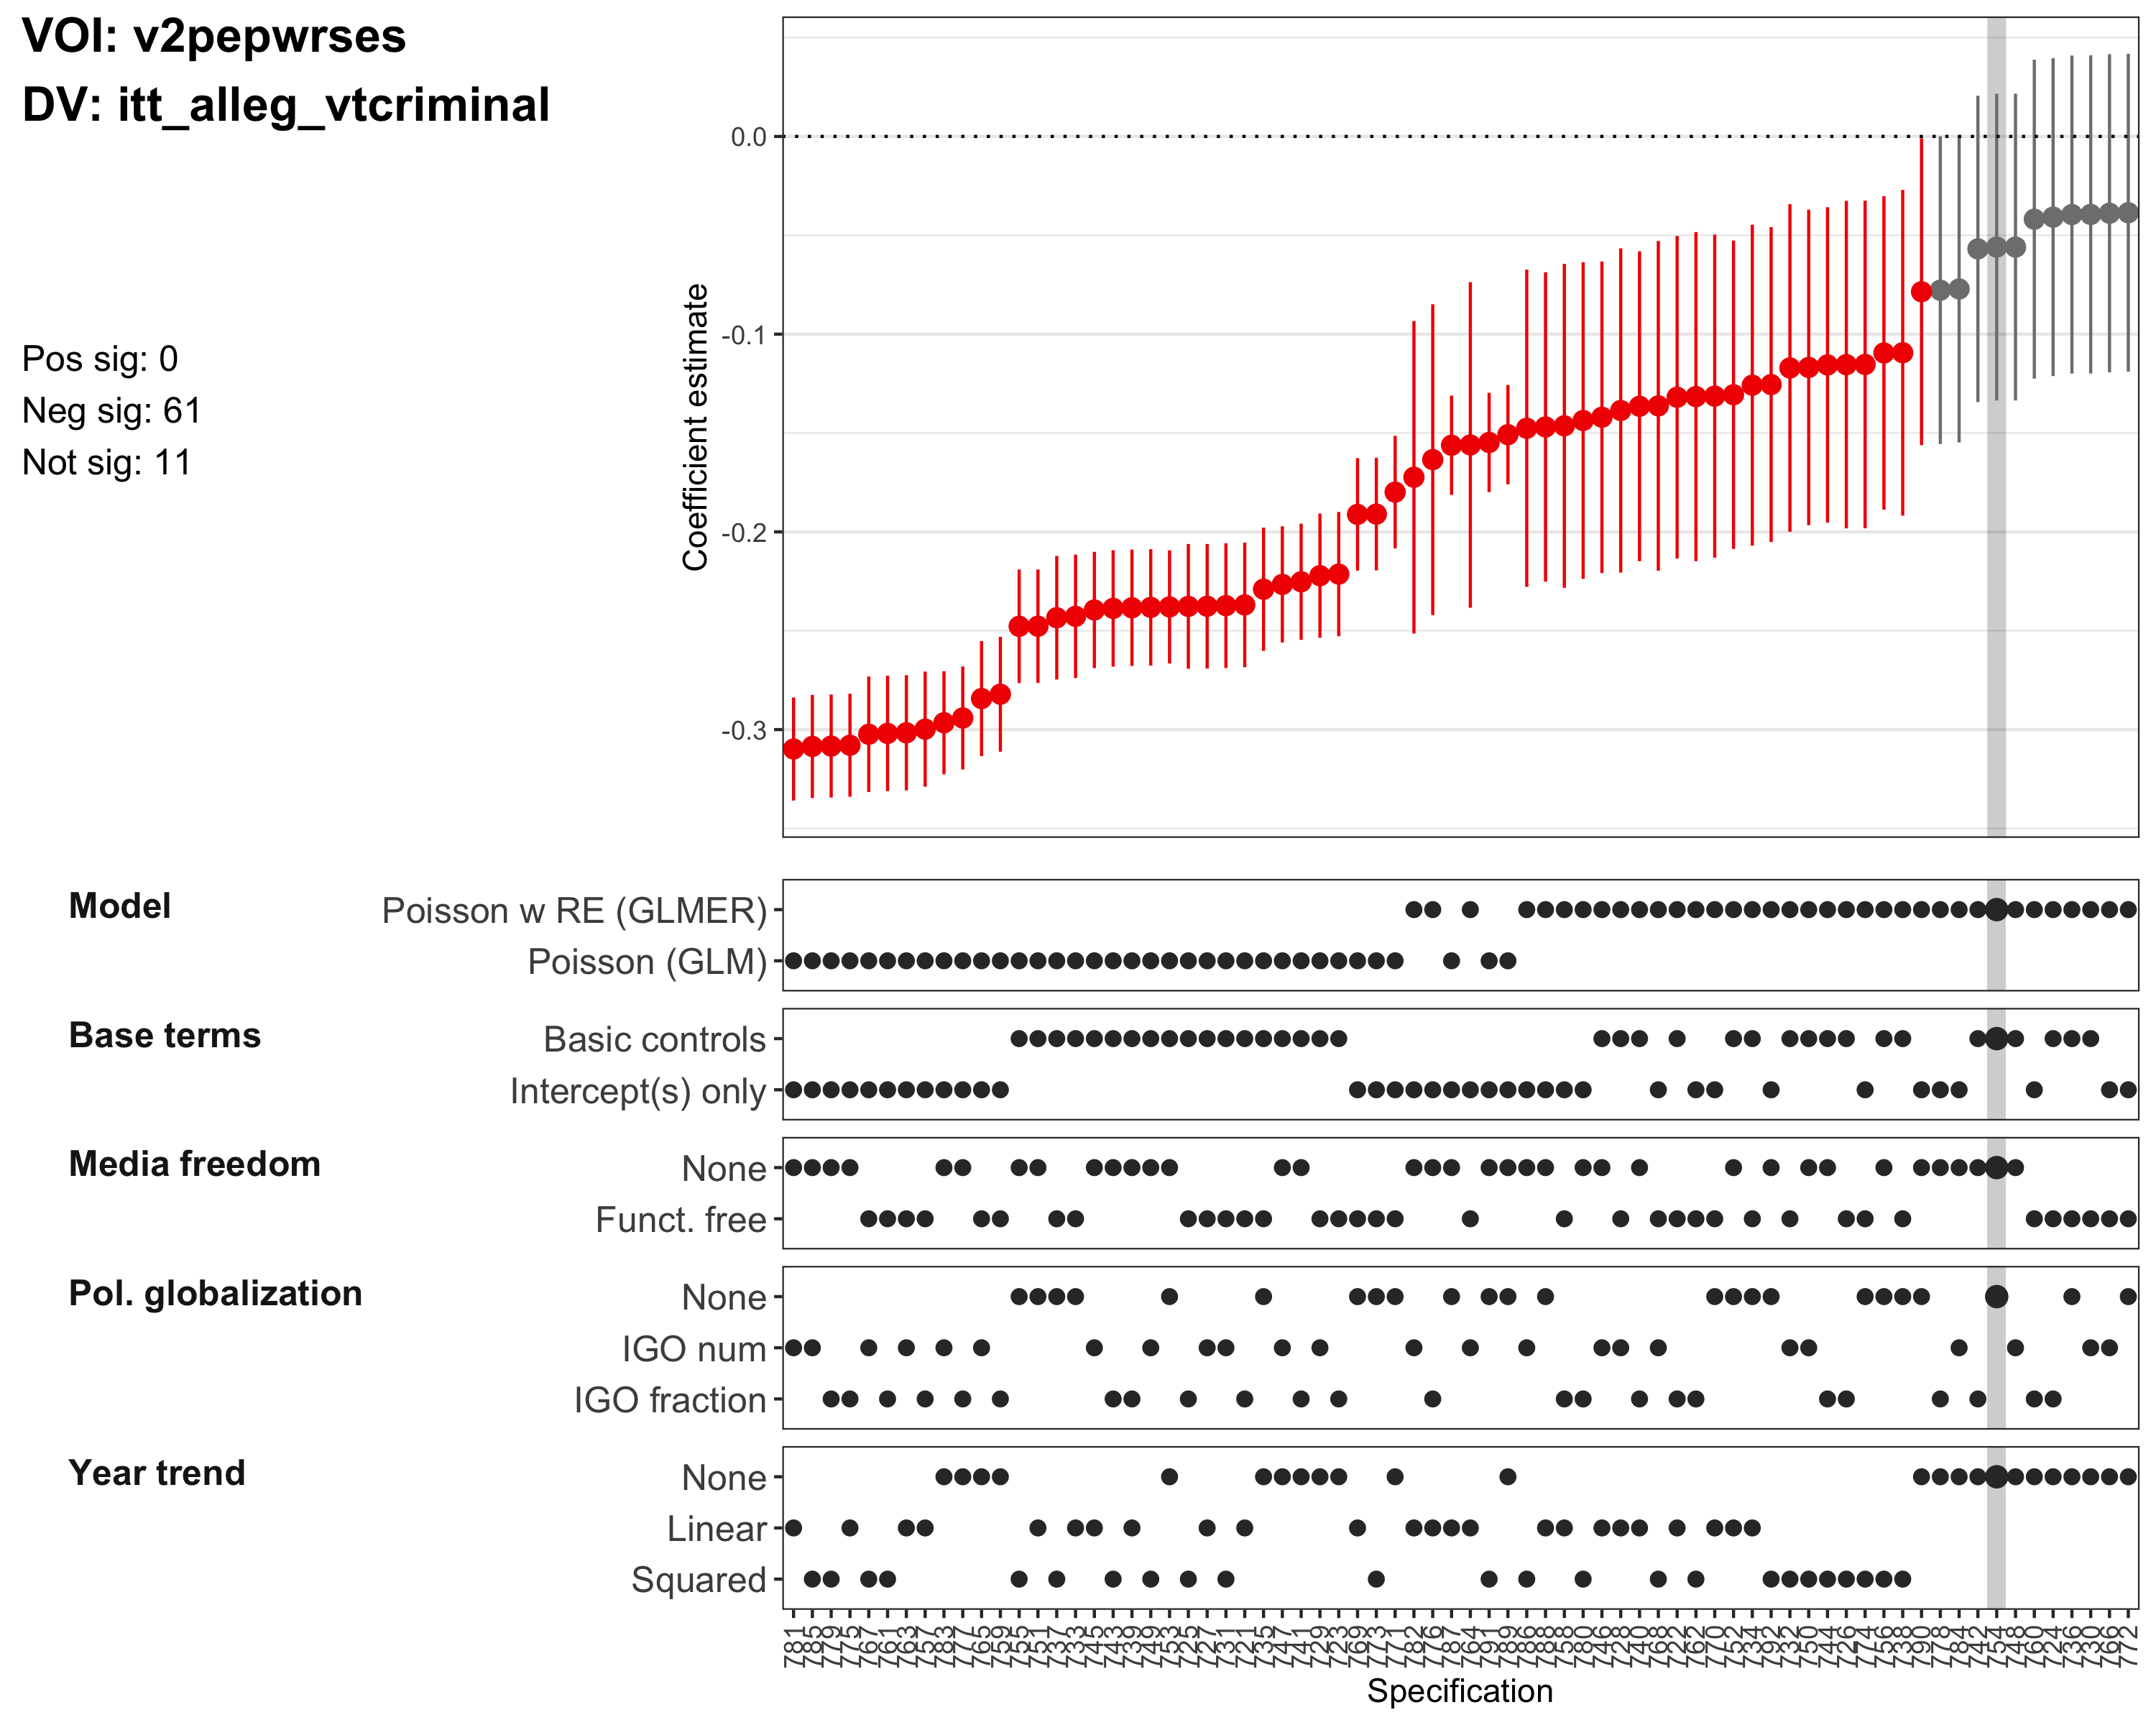
\includegraphics[height=4in]{../output/figures-robustness/specplot-v2pepwrses-itt_alleg_vtcriminal.png}

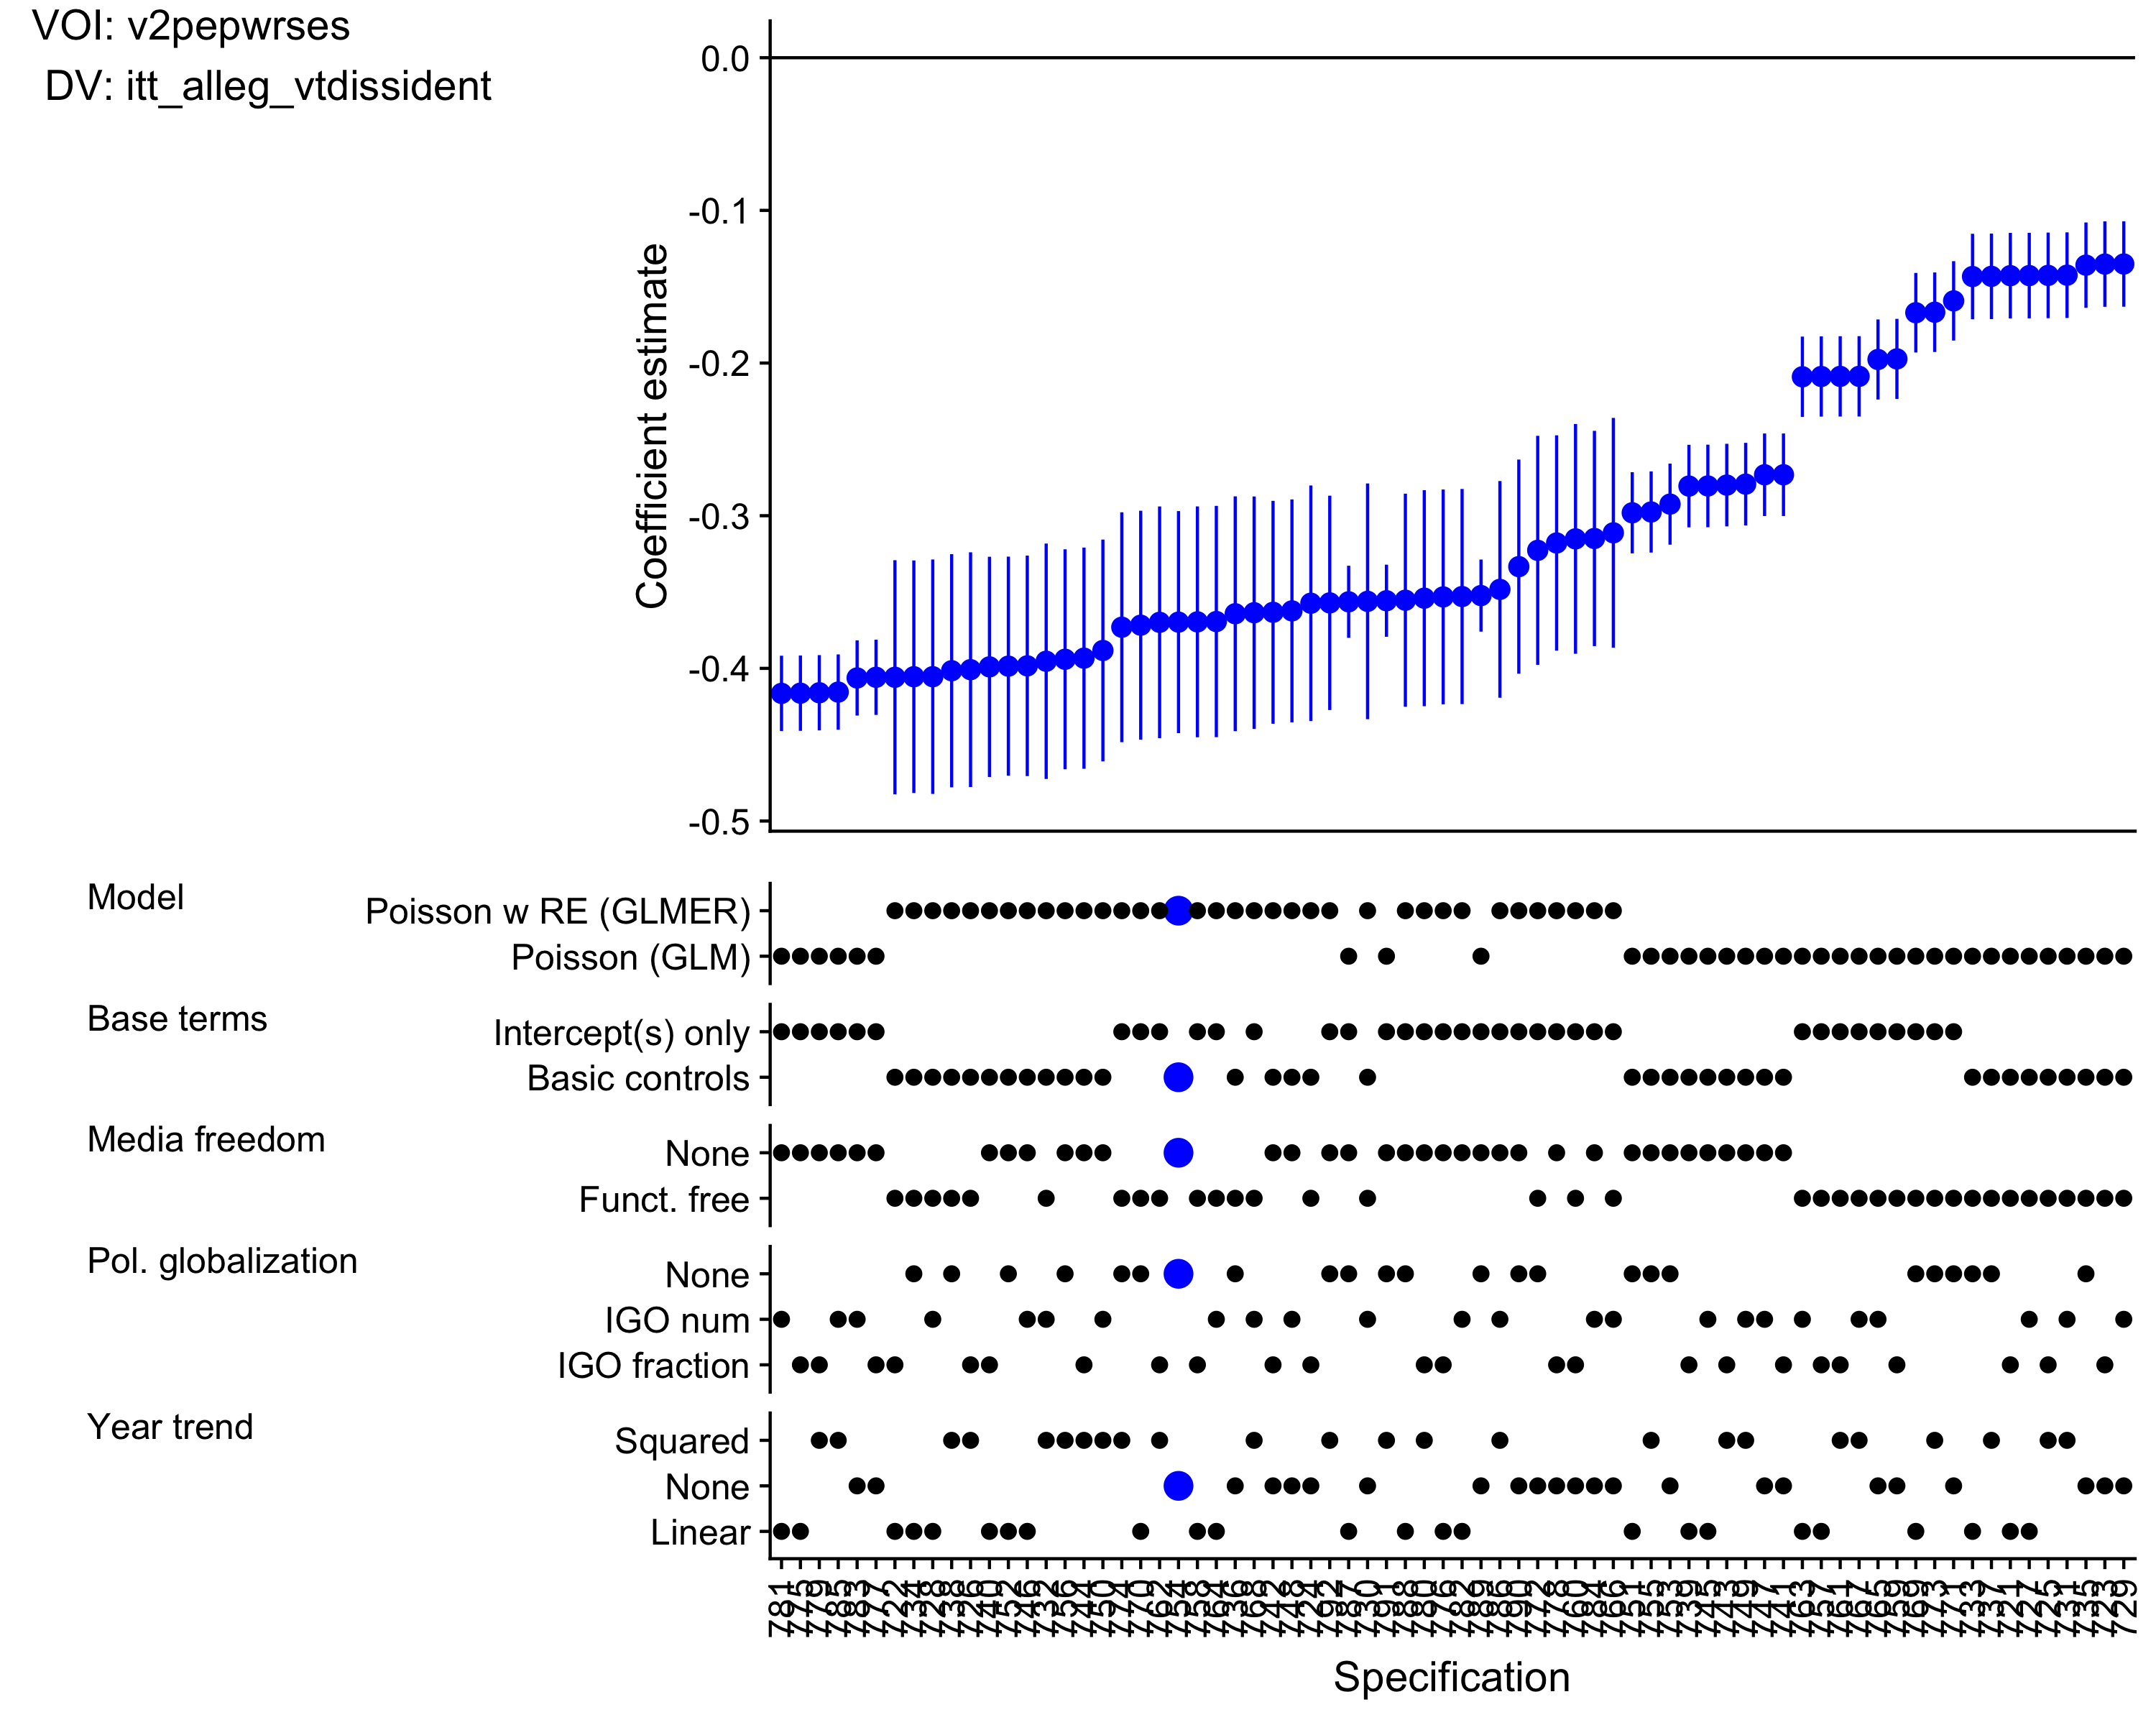
\includegraphics[height=4in]{../output/figures-robustness/specplot-v2pepwrses-itt_alleg_vtdissident.png}

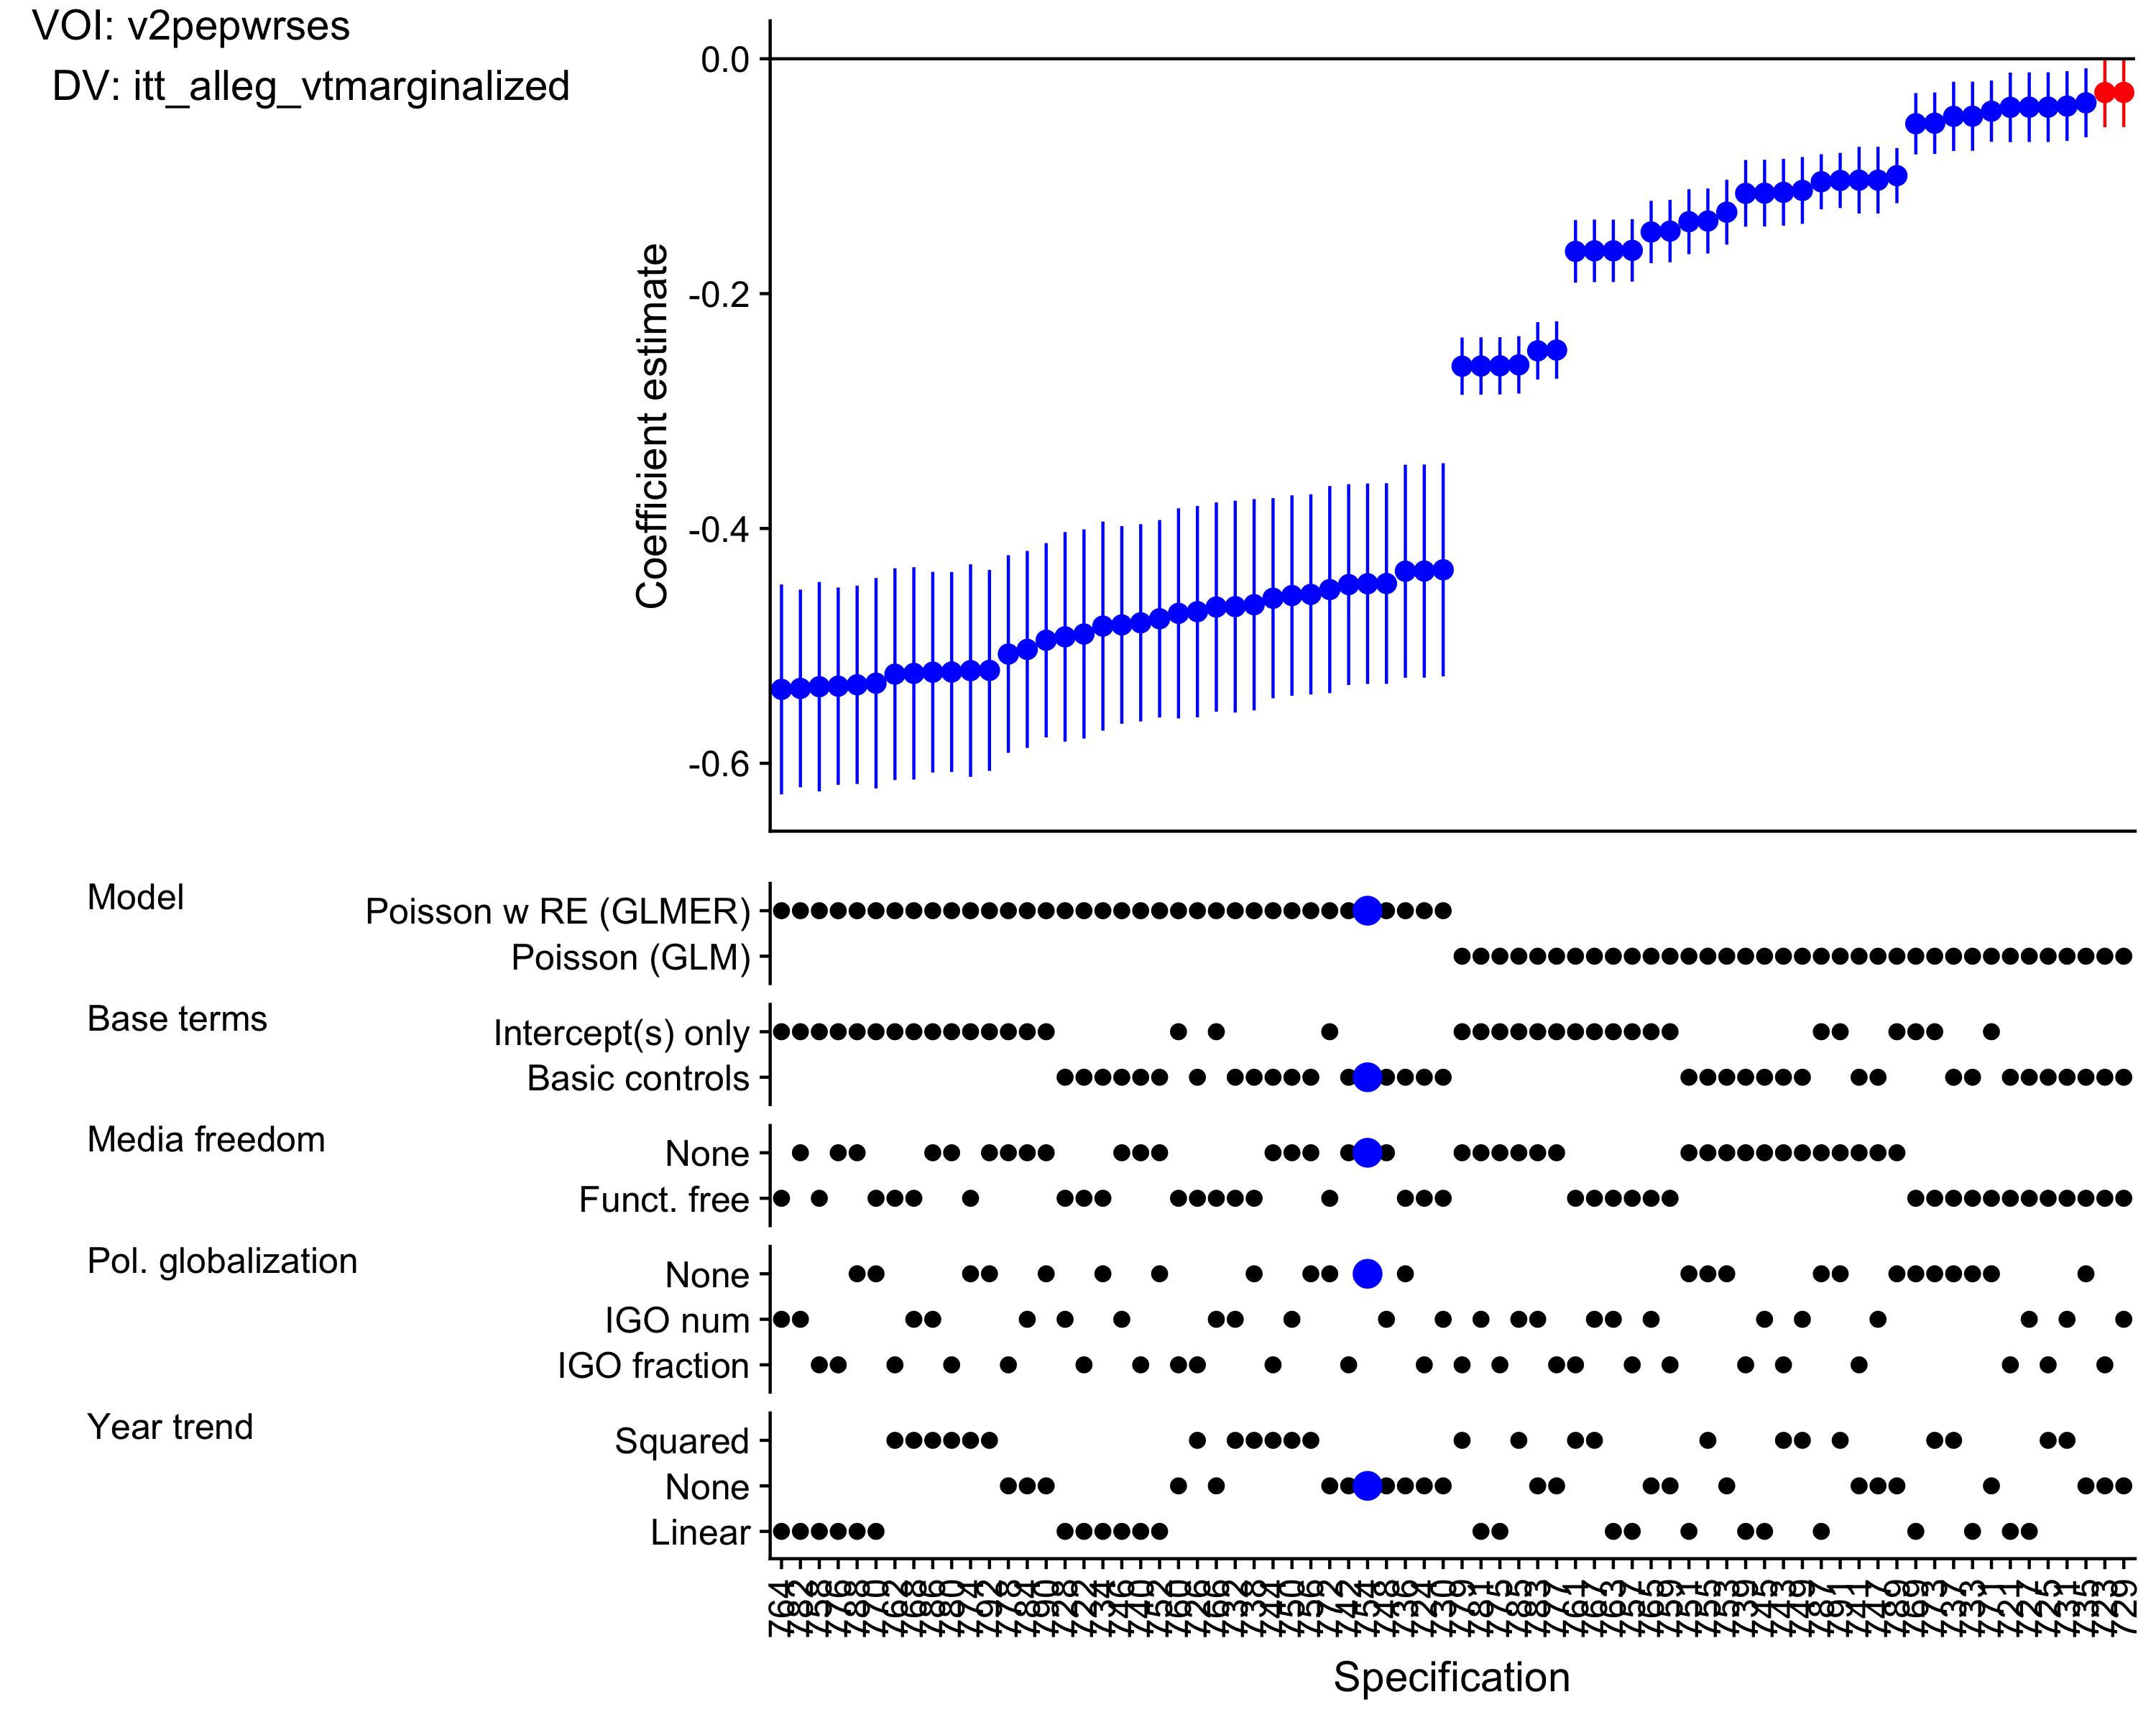
\includegraphics[height=4in]{../output/figures-robustness/specplot-v2pepwrses-itt_alleg_vtmarginalized.png}

\hypertarget{voi-v2pepwrsoc}{%
\subsection{VOI: v2pepwrsoc}\label{voi-v2pepwrsoc}}

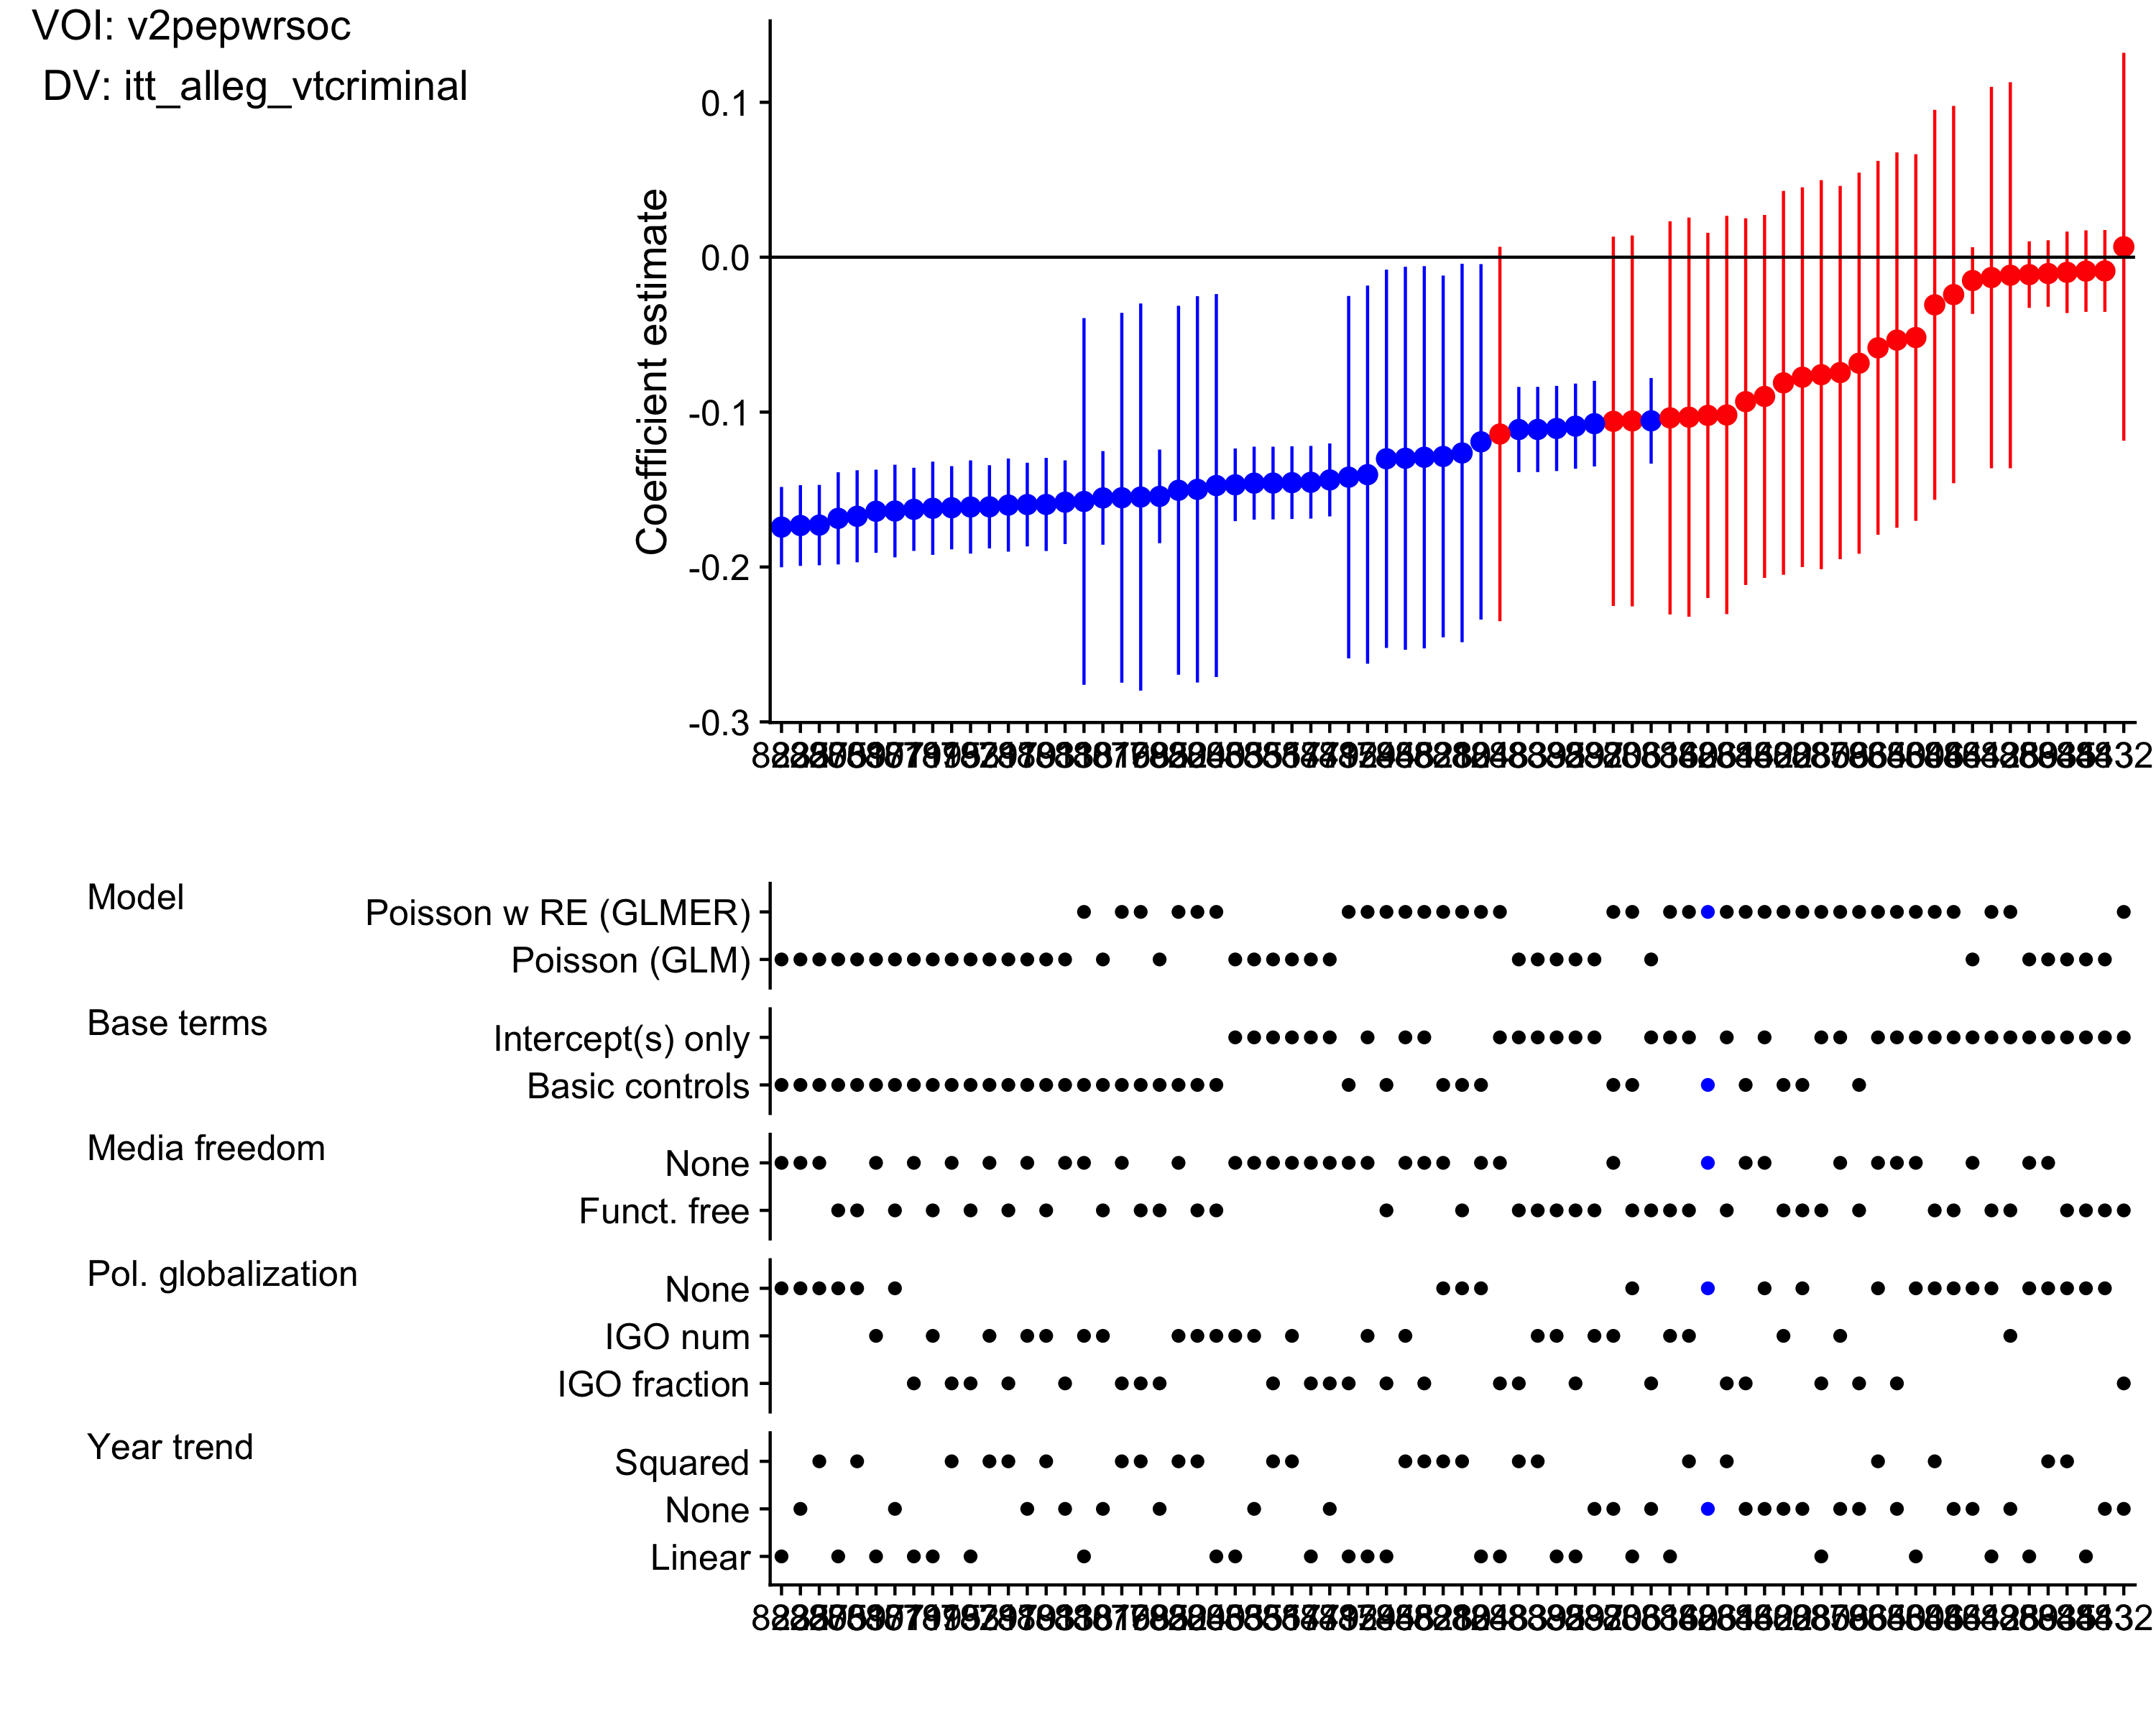
\includegraphics[height=4in]{../output/figures-robustness/specplot-v2pepwrsoc-itt_alleg_vtcriminal.png}

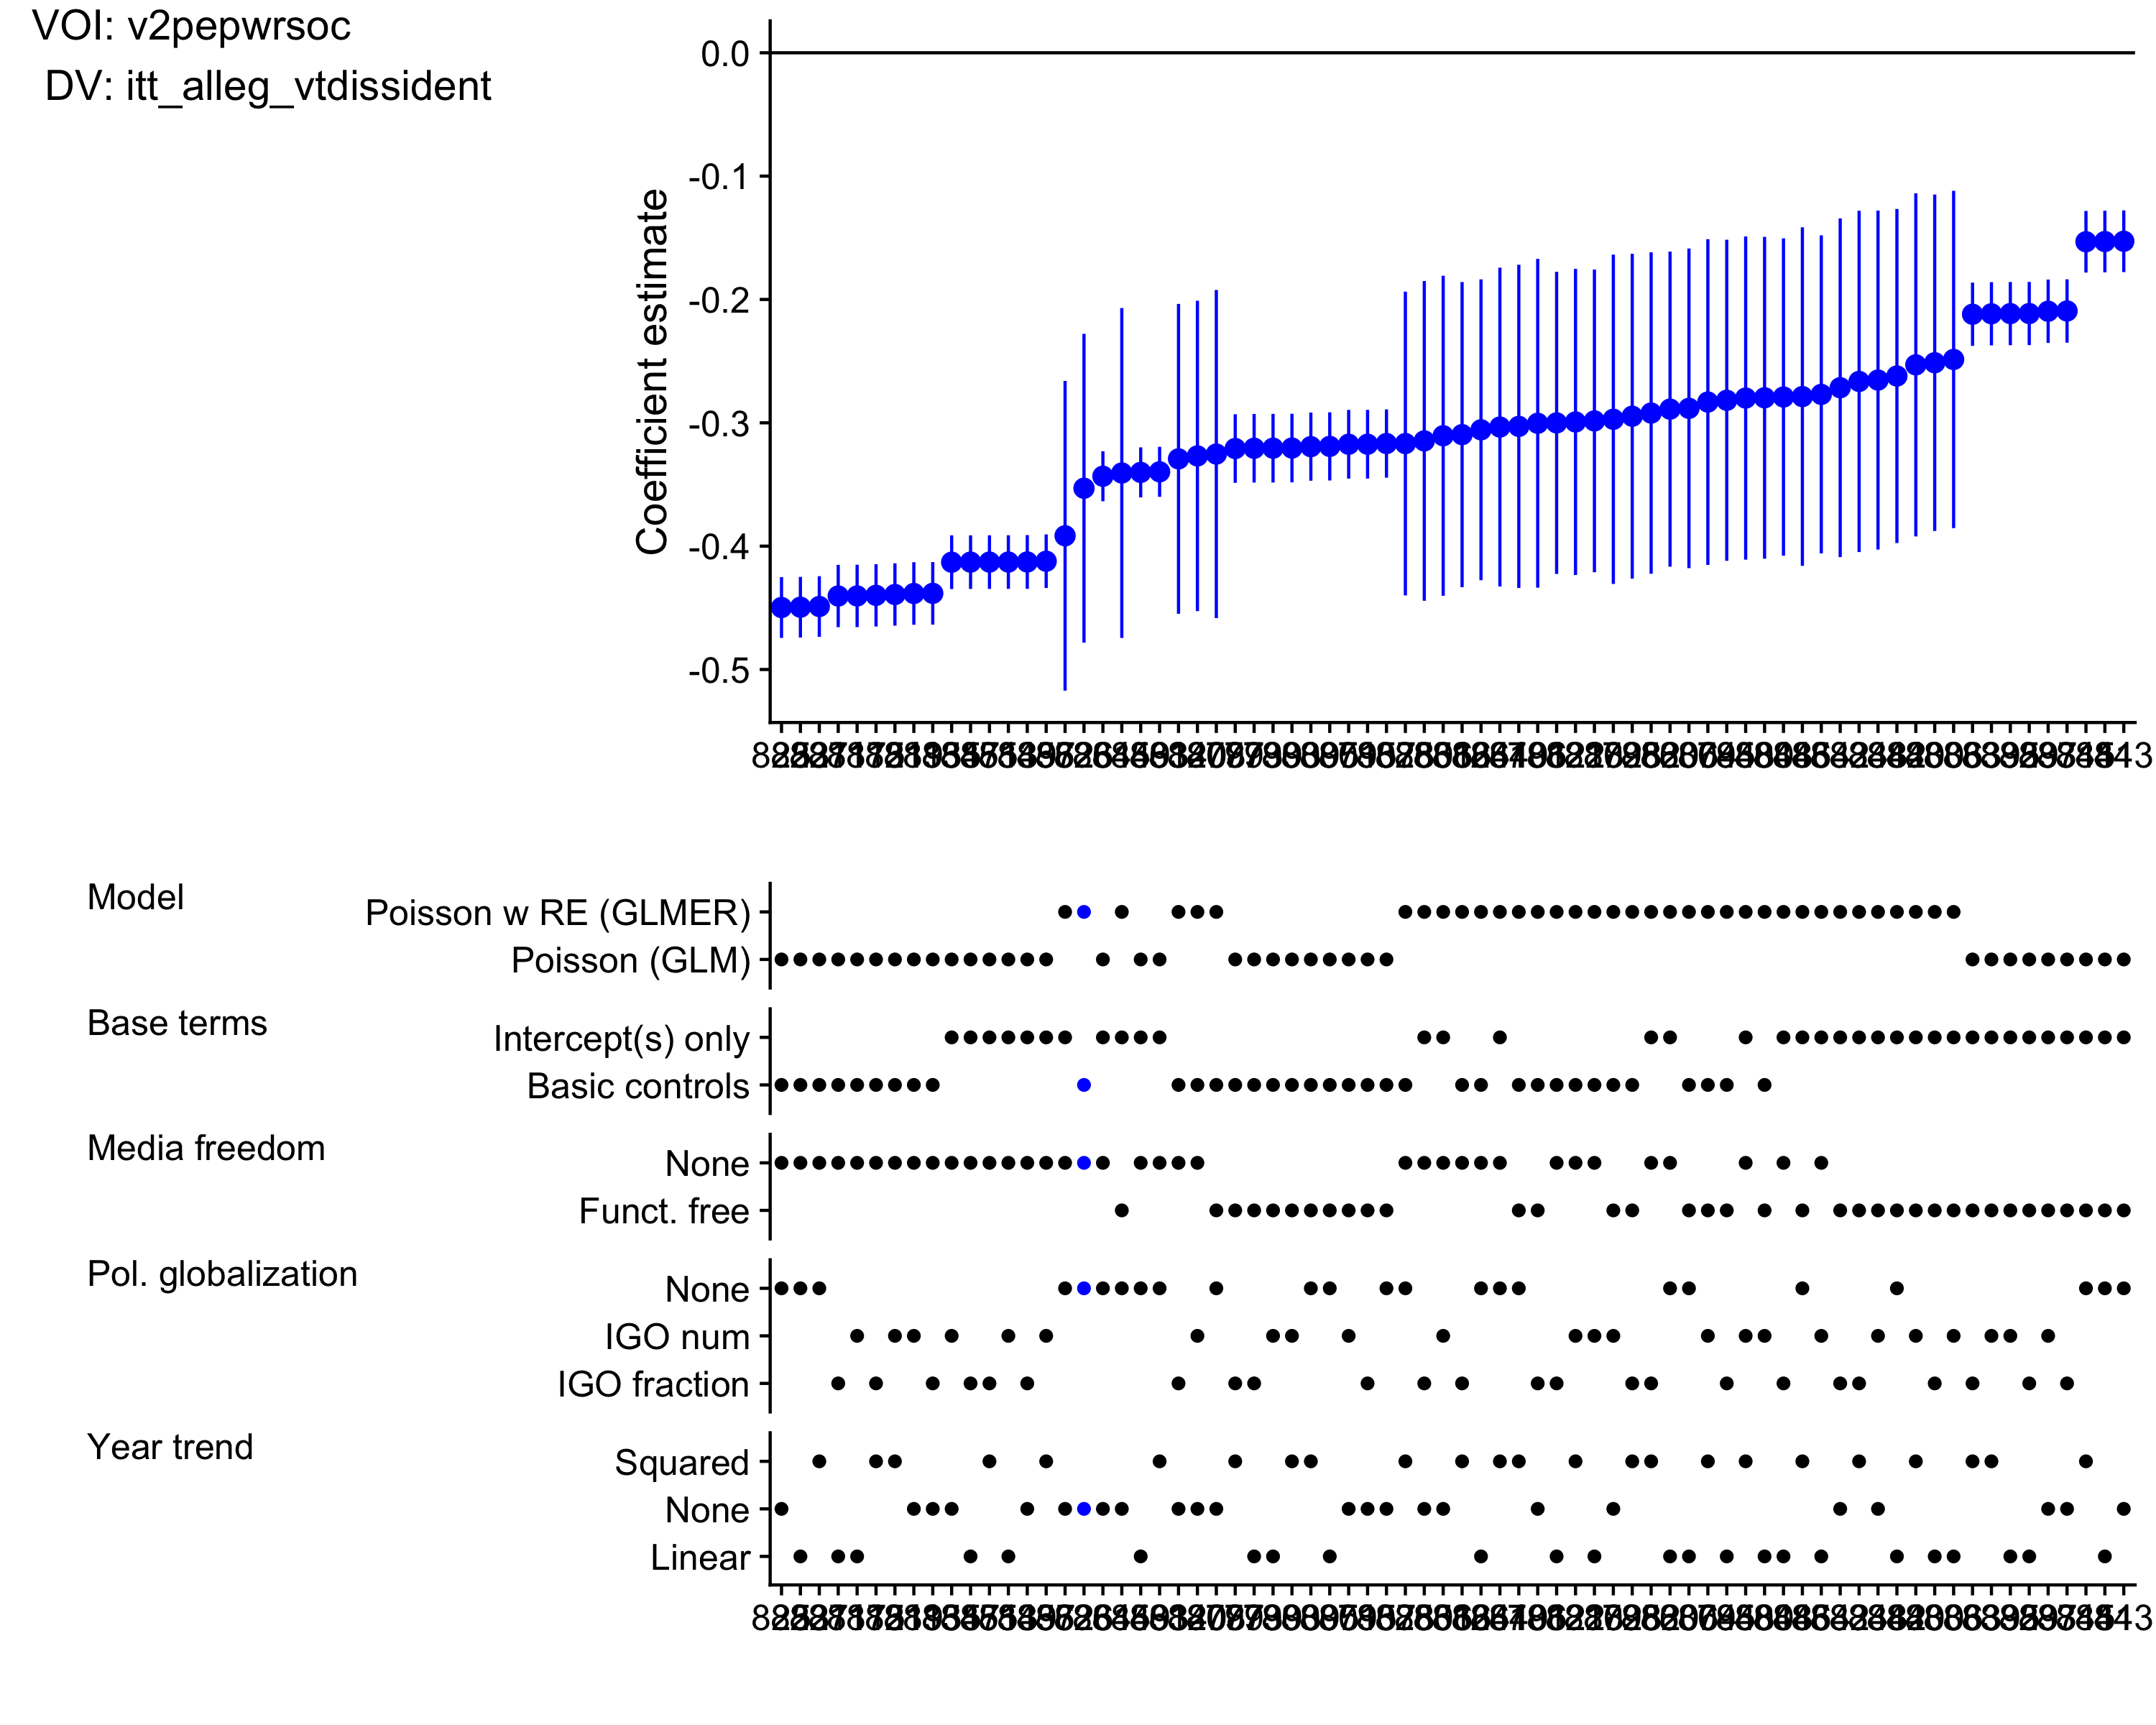
\includegraphics[height=4in]{../output/figures-robustness/specplot-v2pepwrsoc-itt_alleg_vtdissident.png}

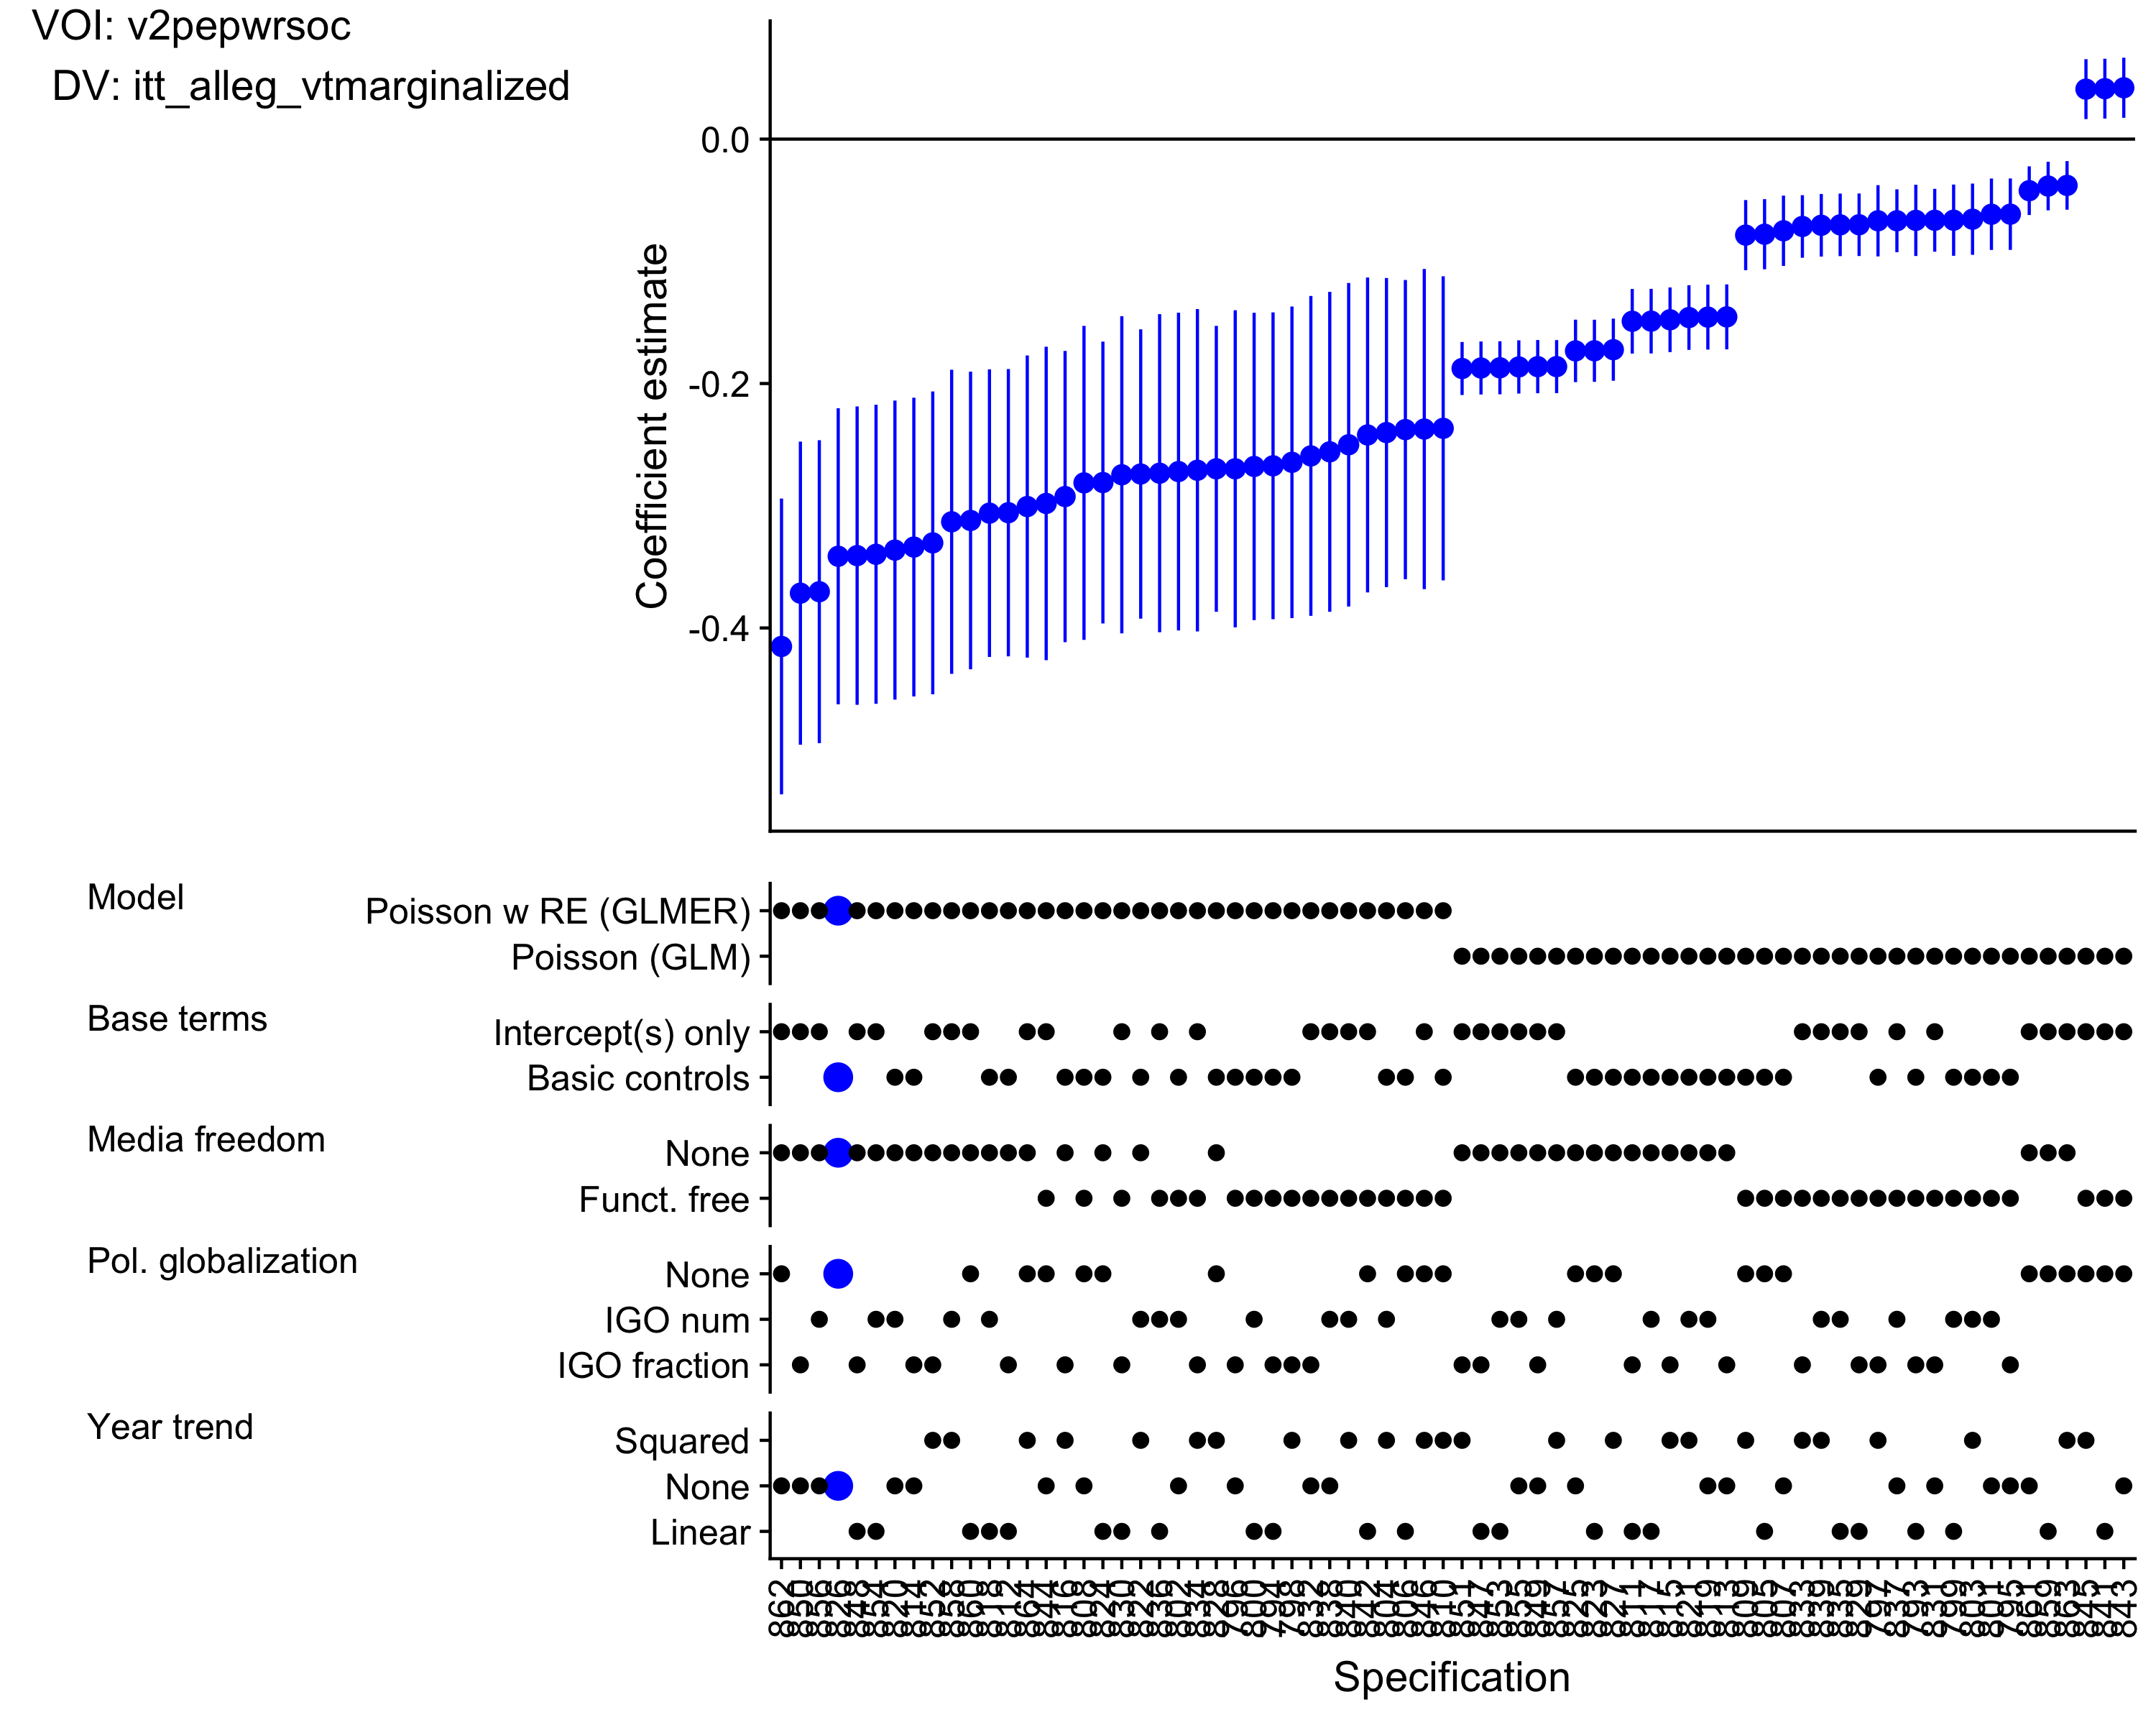
\includegraphics[height=4in]{../output/figures-robustness/specplot-v2pepwrsoc-itt_alleg_vtmarginalized.png}

\hypertarget{voi-v2x_jucon}{%
\subsection{VOI: v2x\_jucon}\label{voi-v2x_jucon}}

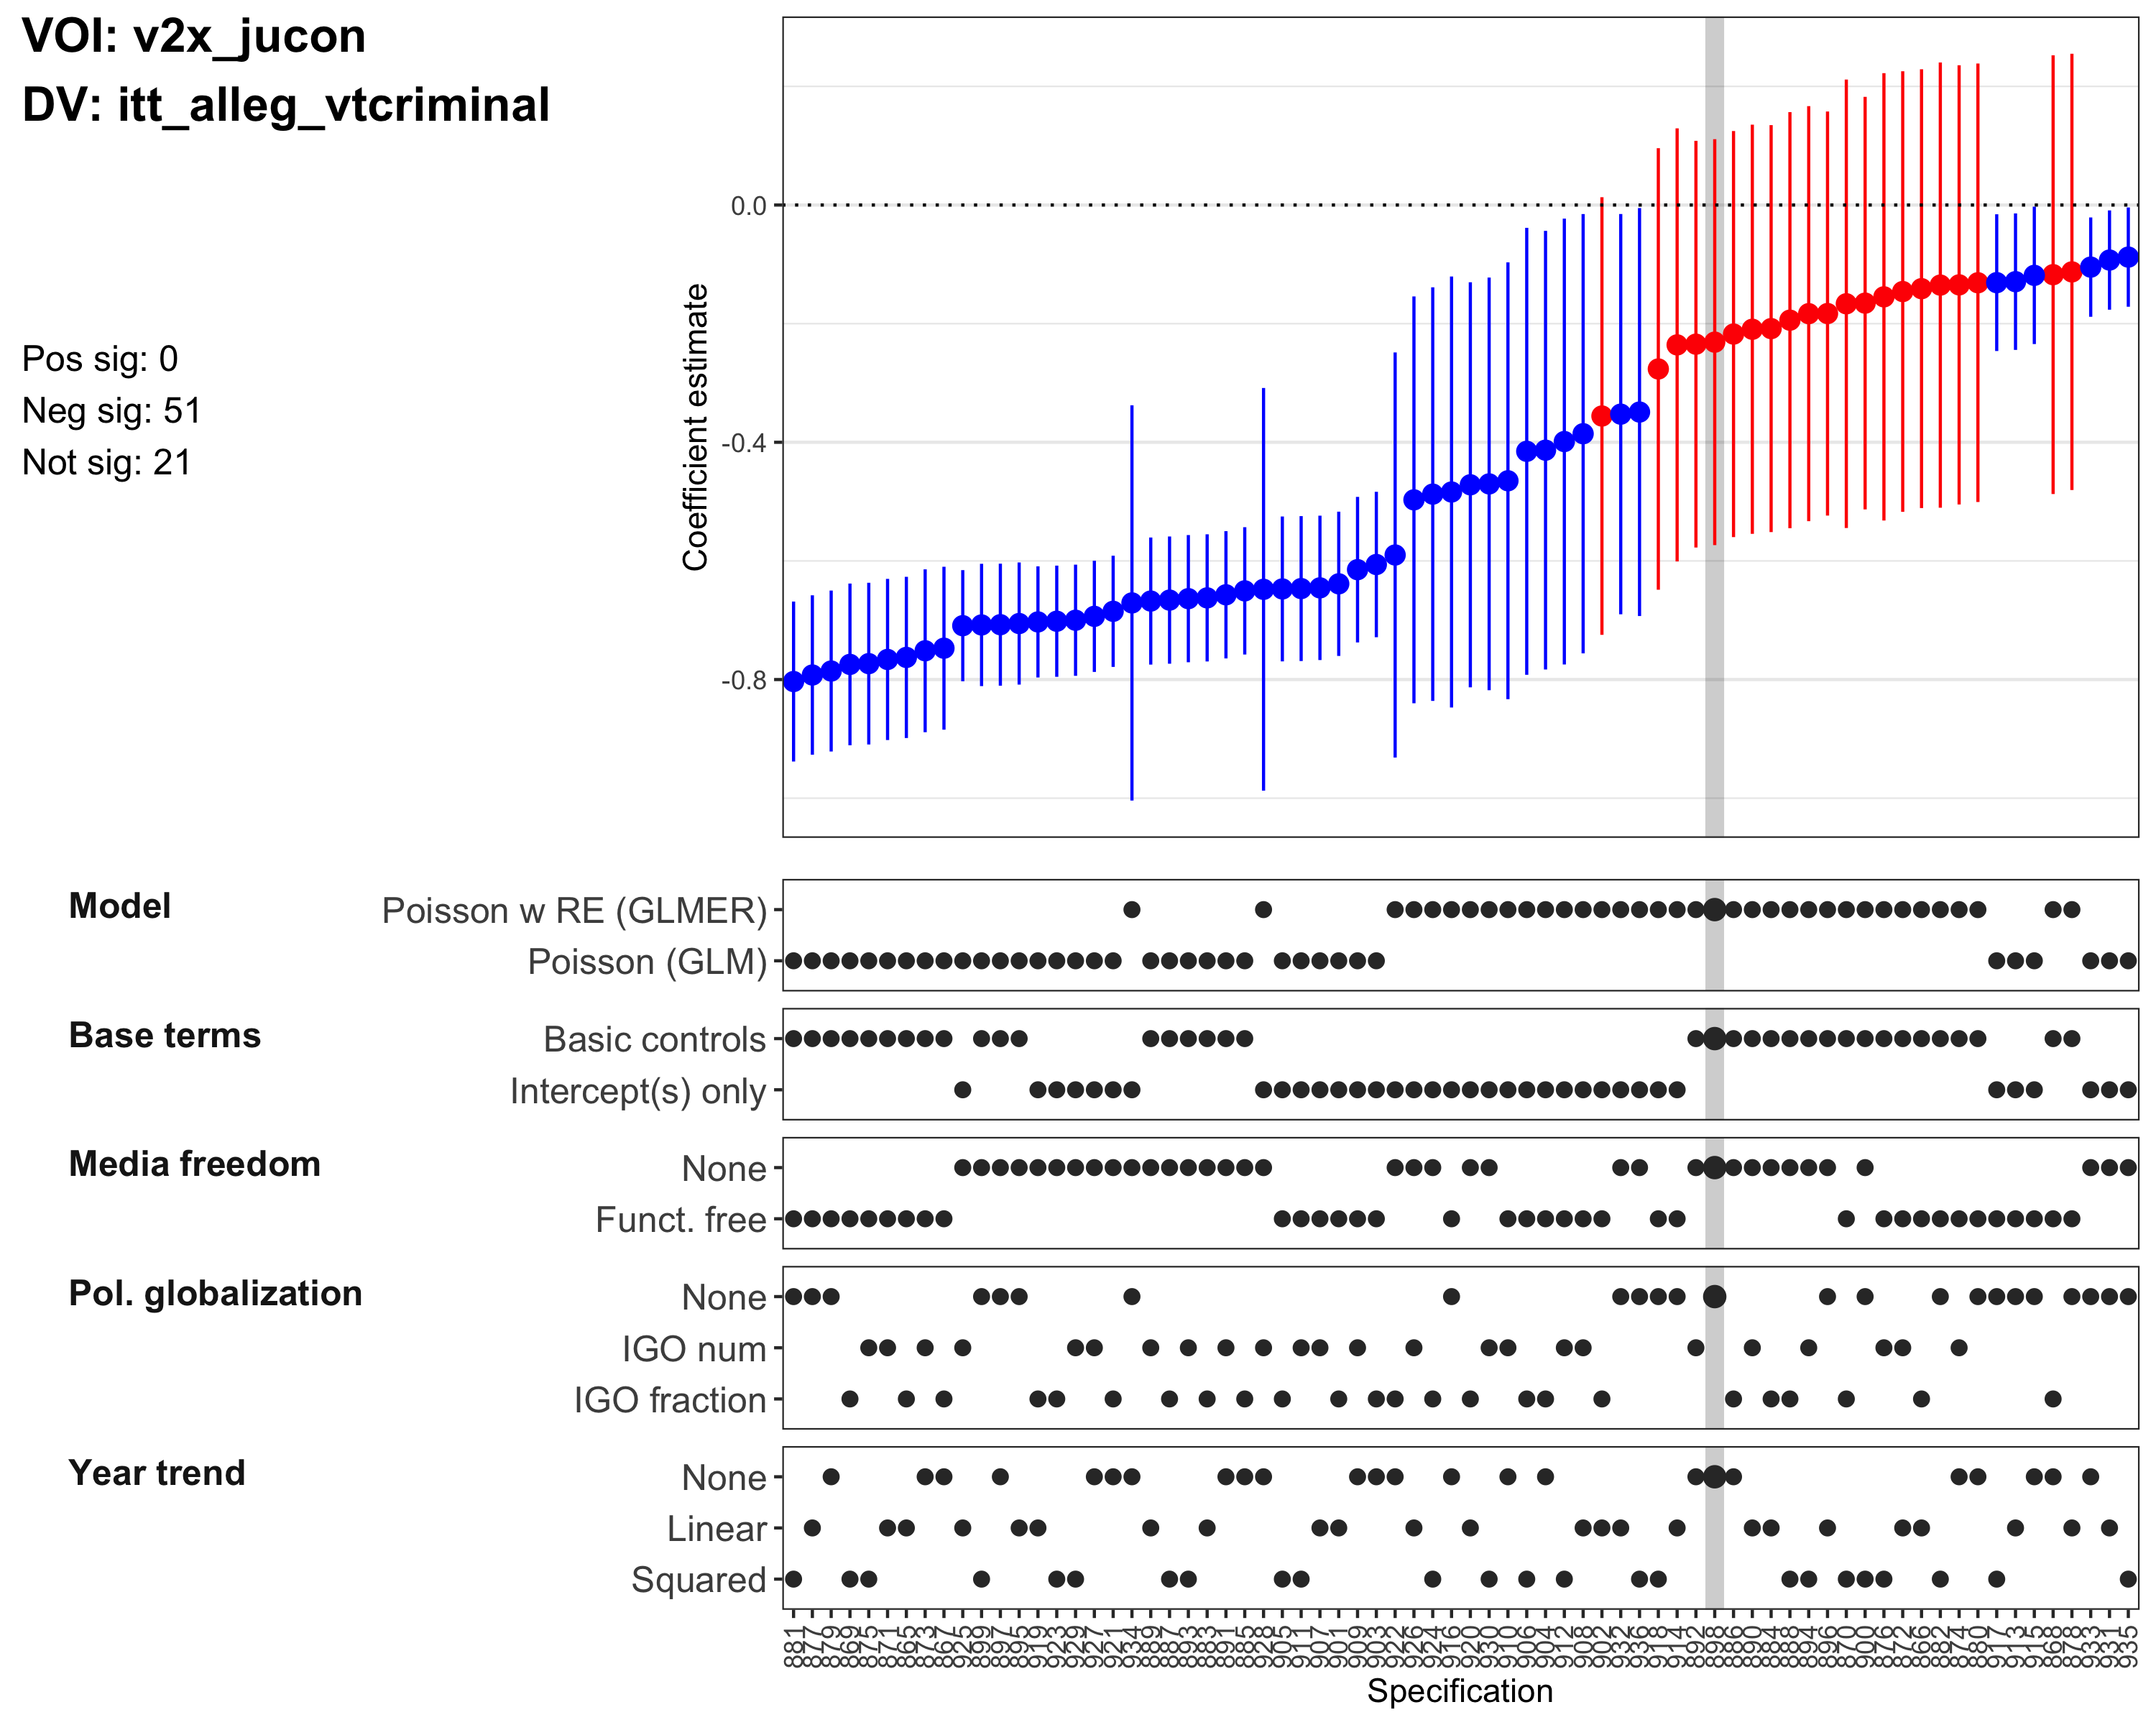
\includegraphics[height=4in]{../output/figures-robustness/specplot-v2x_jucon-itt_alleg_vtcriminal.png}

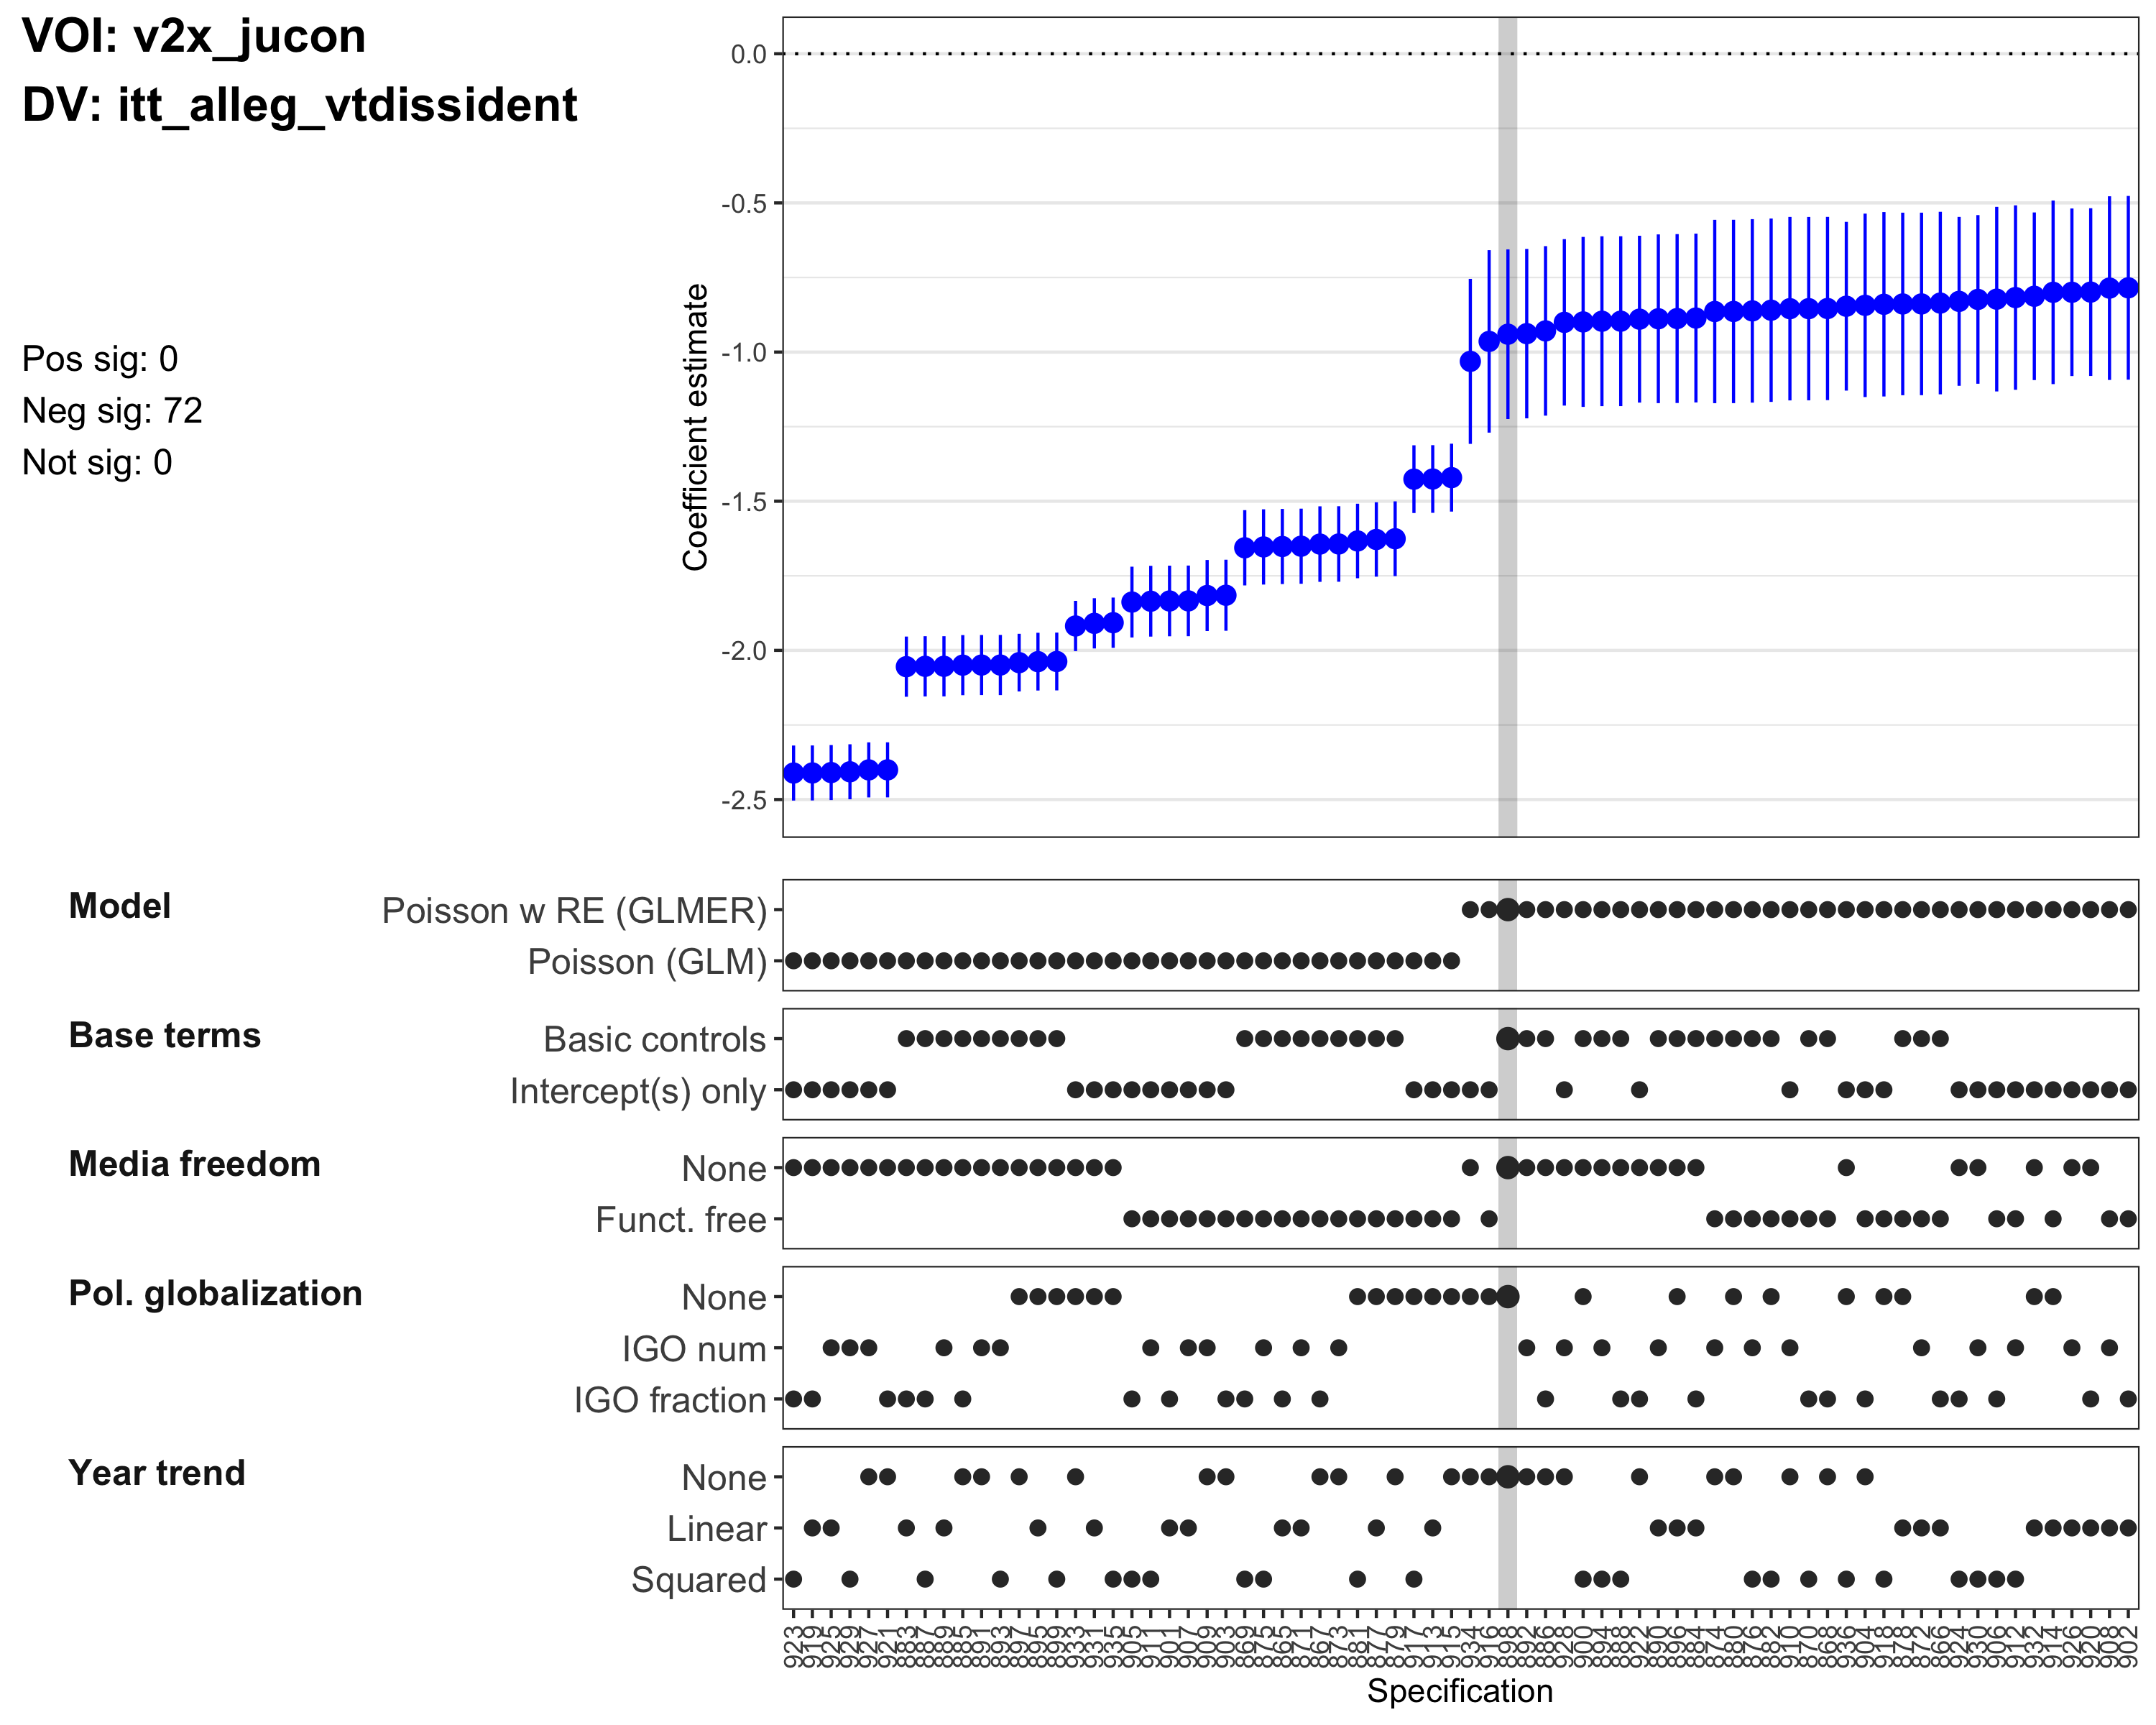
\includegraphics[height=4in]{../output/figures-robustness/specplot-v2x_jucon-itt_alleg_vtdissident.png}

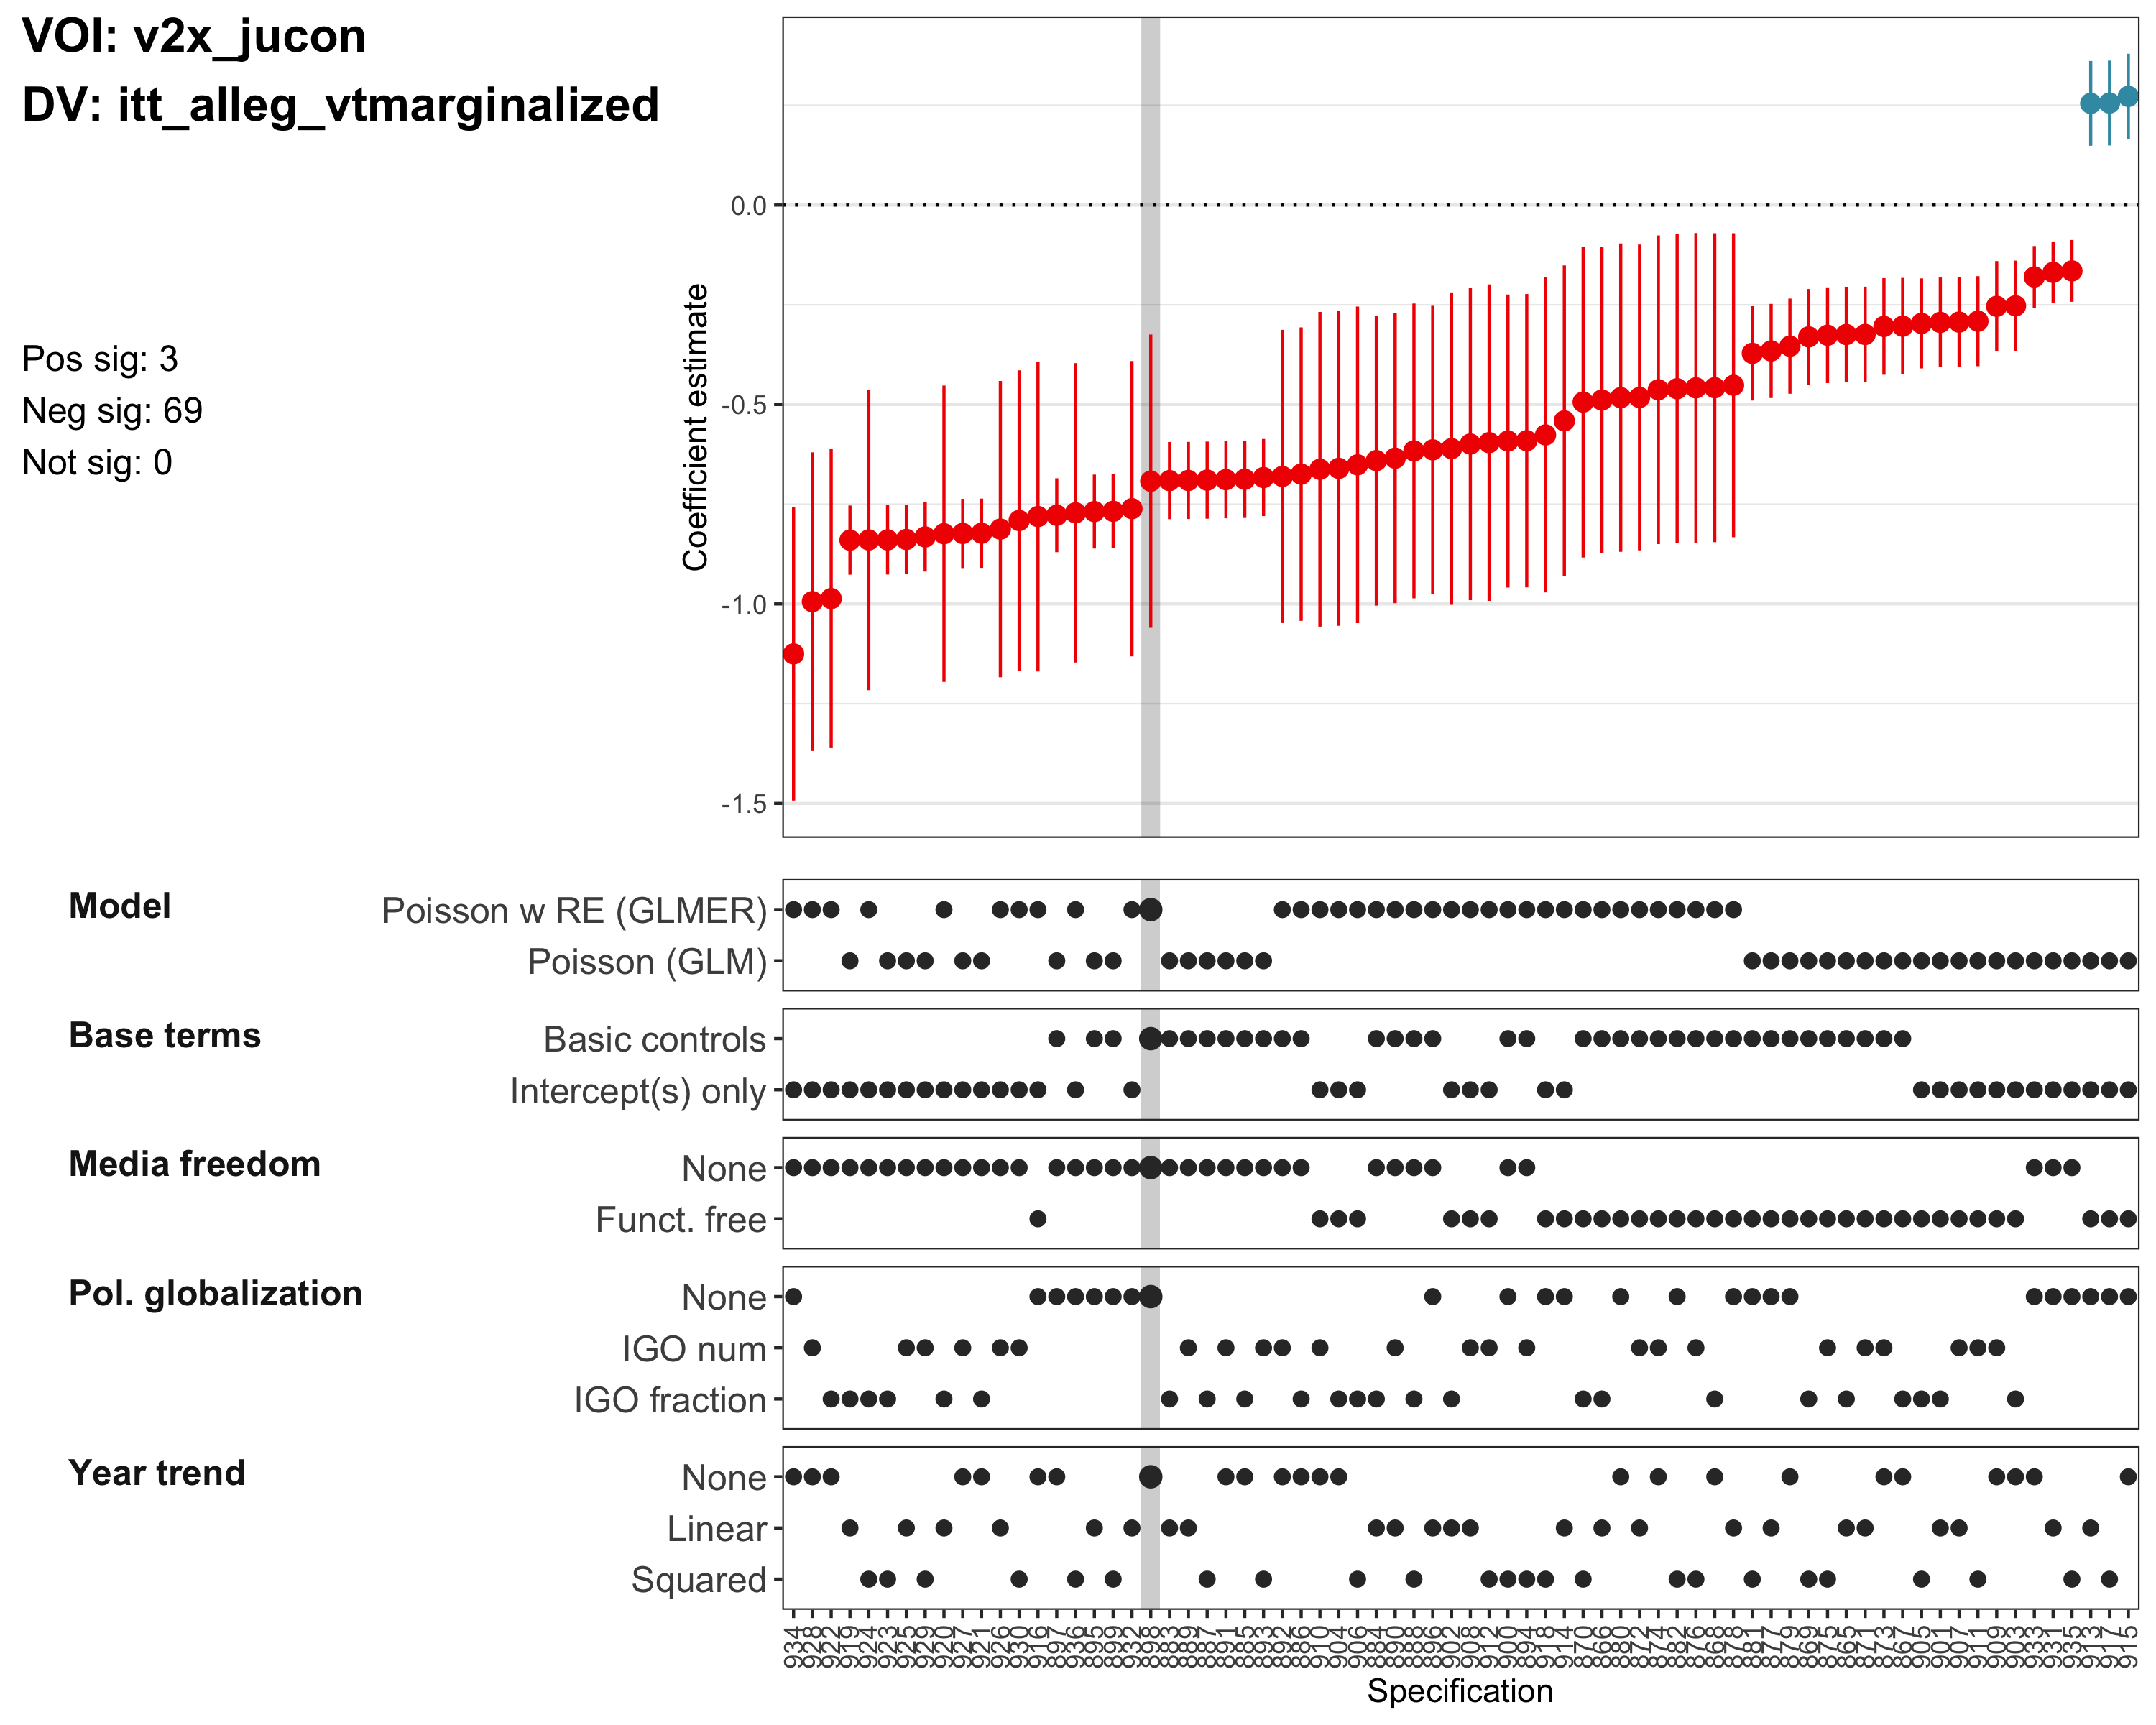
\includegraphics[height=4in]{../output/figures-robustness/specplot-v2x_jucon-itt_alleg_vtmarginalized.png}

\hypertarget{voi-v2xlg_legcon}{%
\subsection{VOI: v2xlg\_legcon}\label{voi-v2xlg_legcon}}

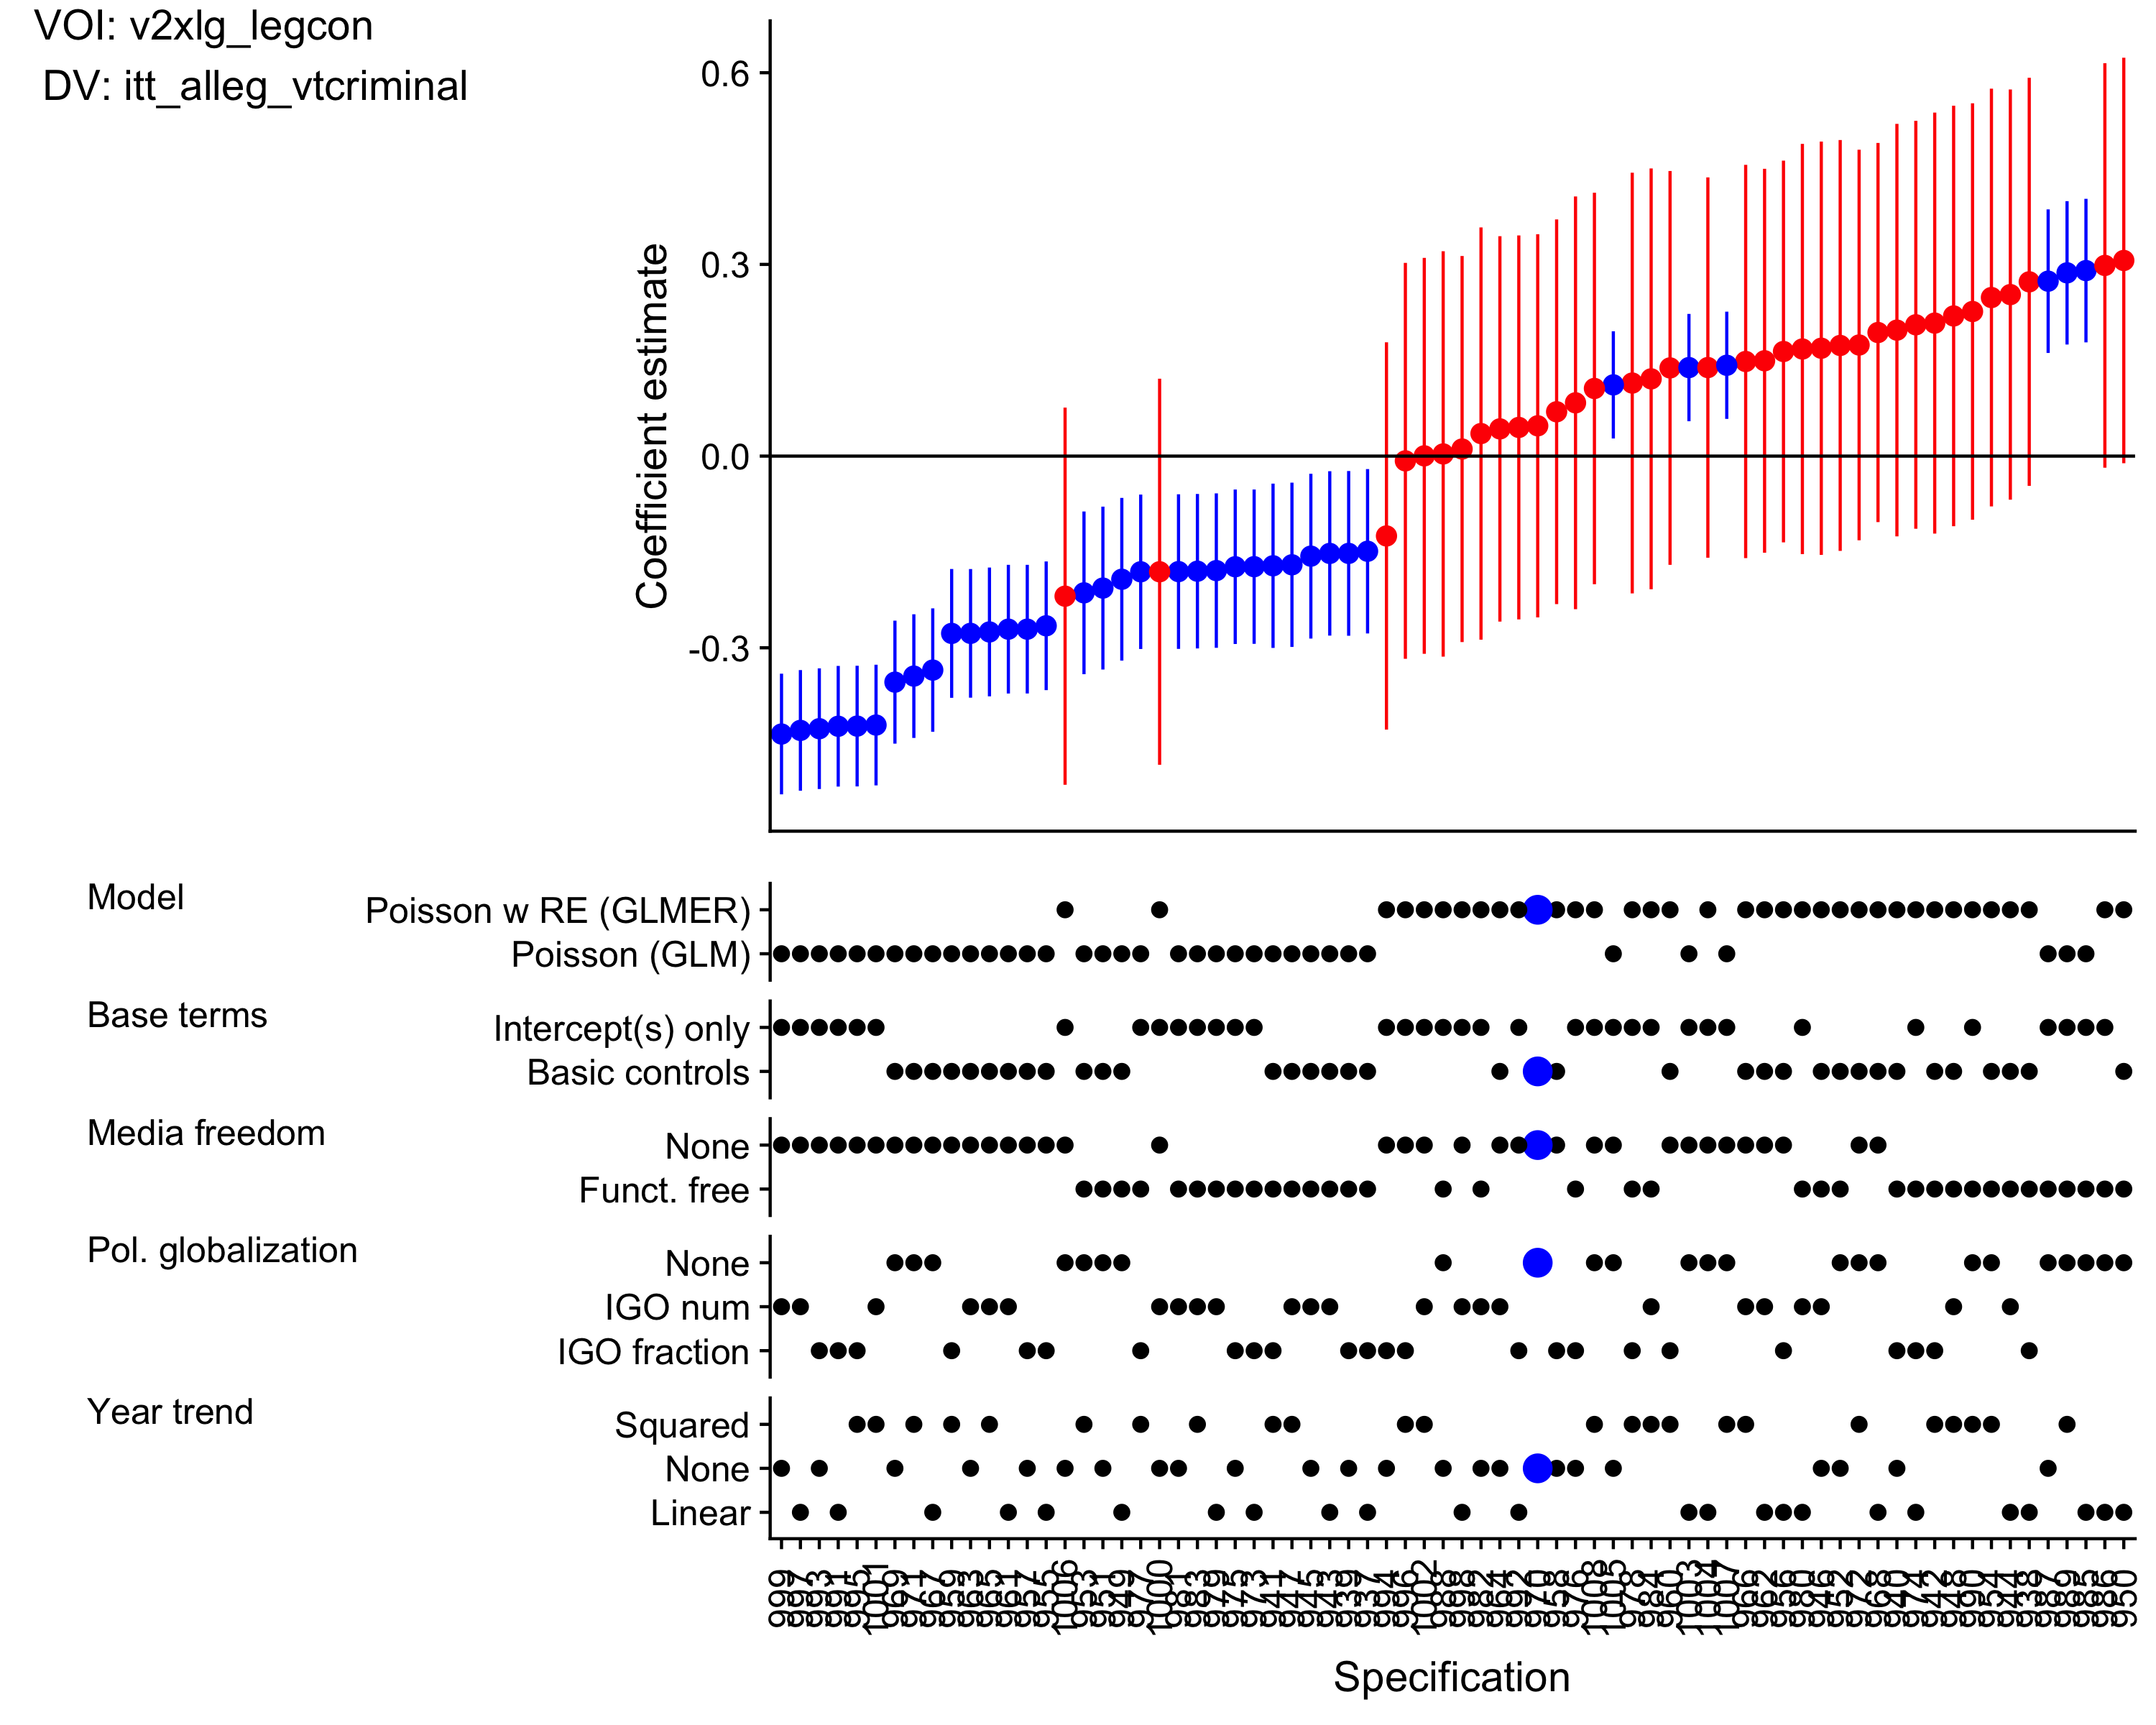
\includegraphics[height=4in]{../output/figures-robustness/specplot-v2xlg_legcon-itt_alleg_vtcriminal.png}

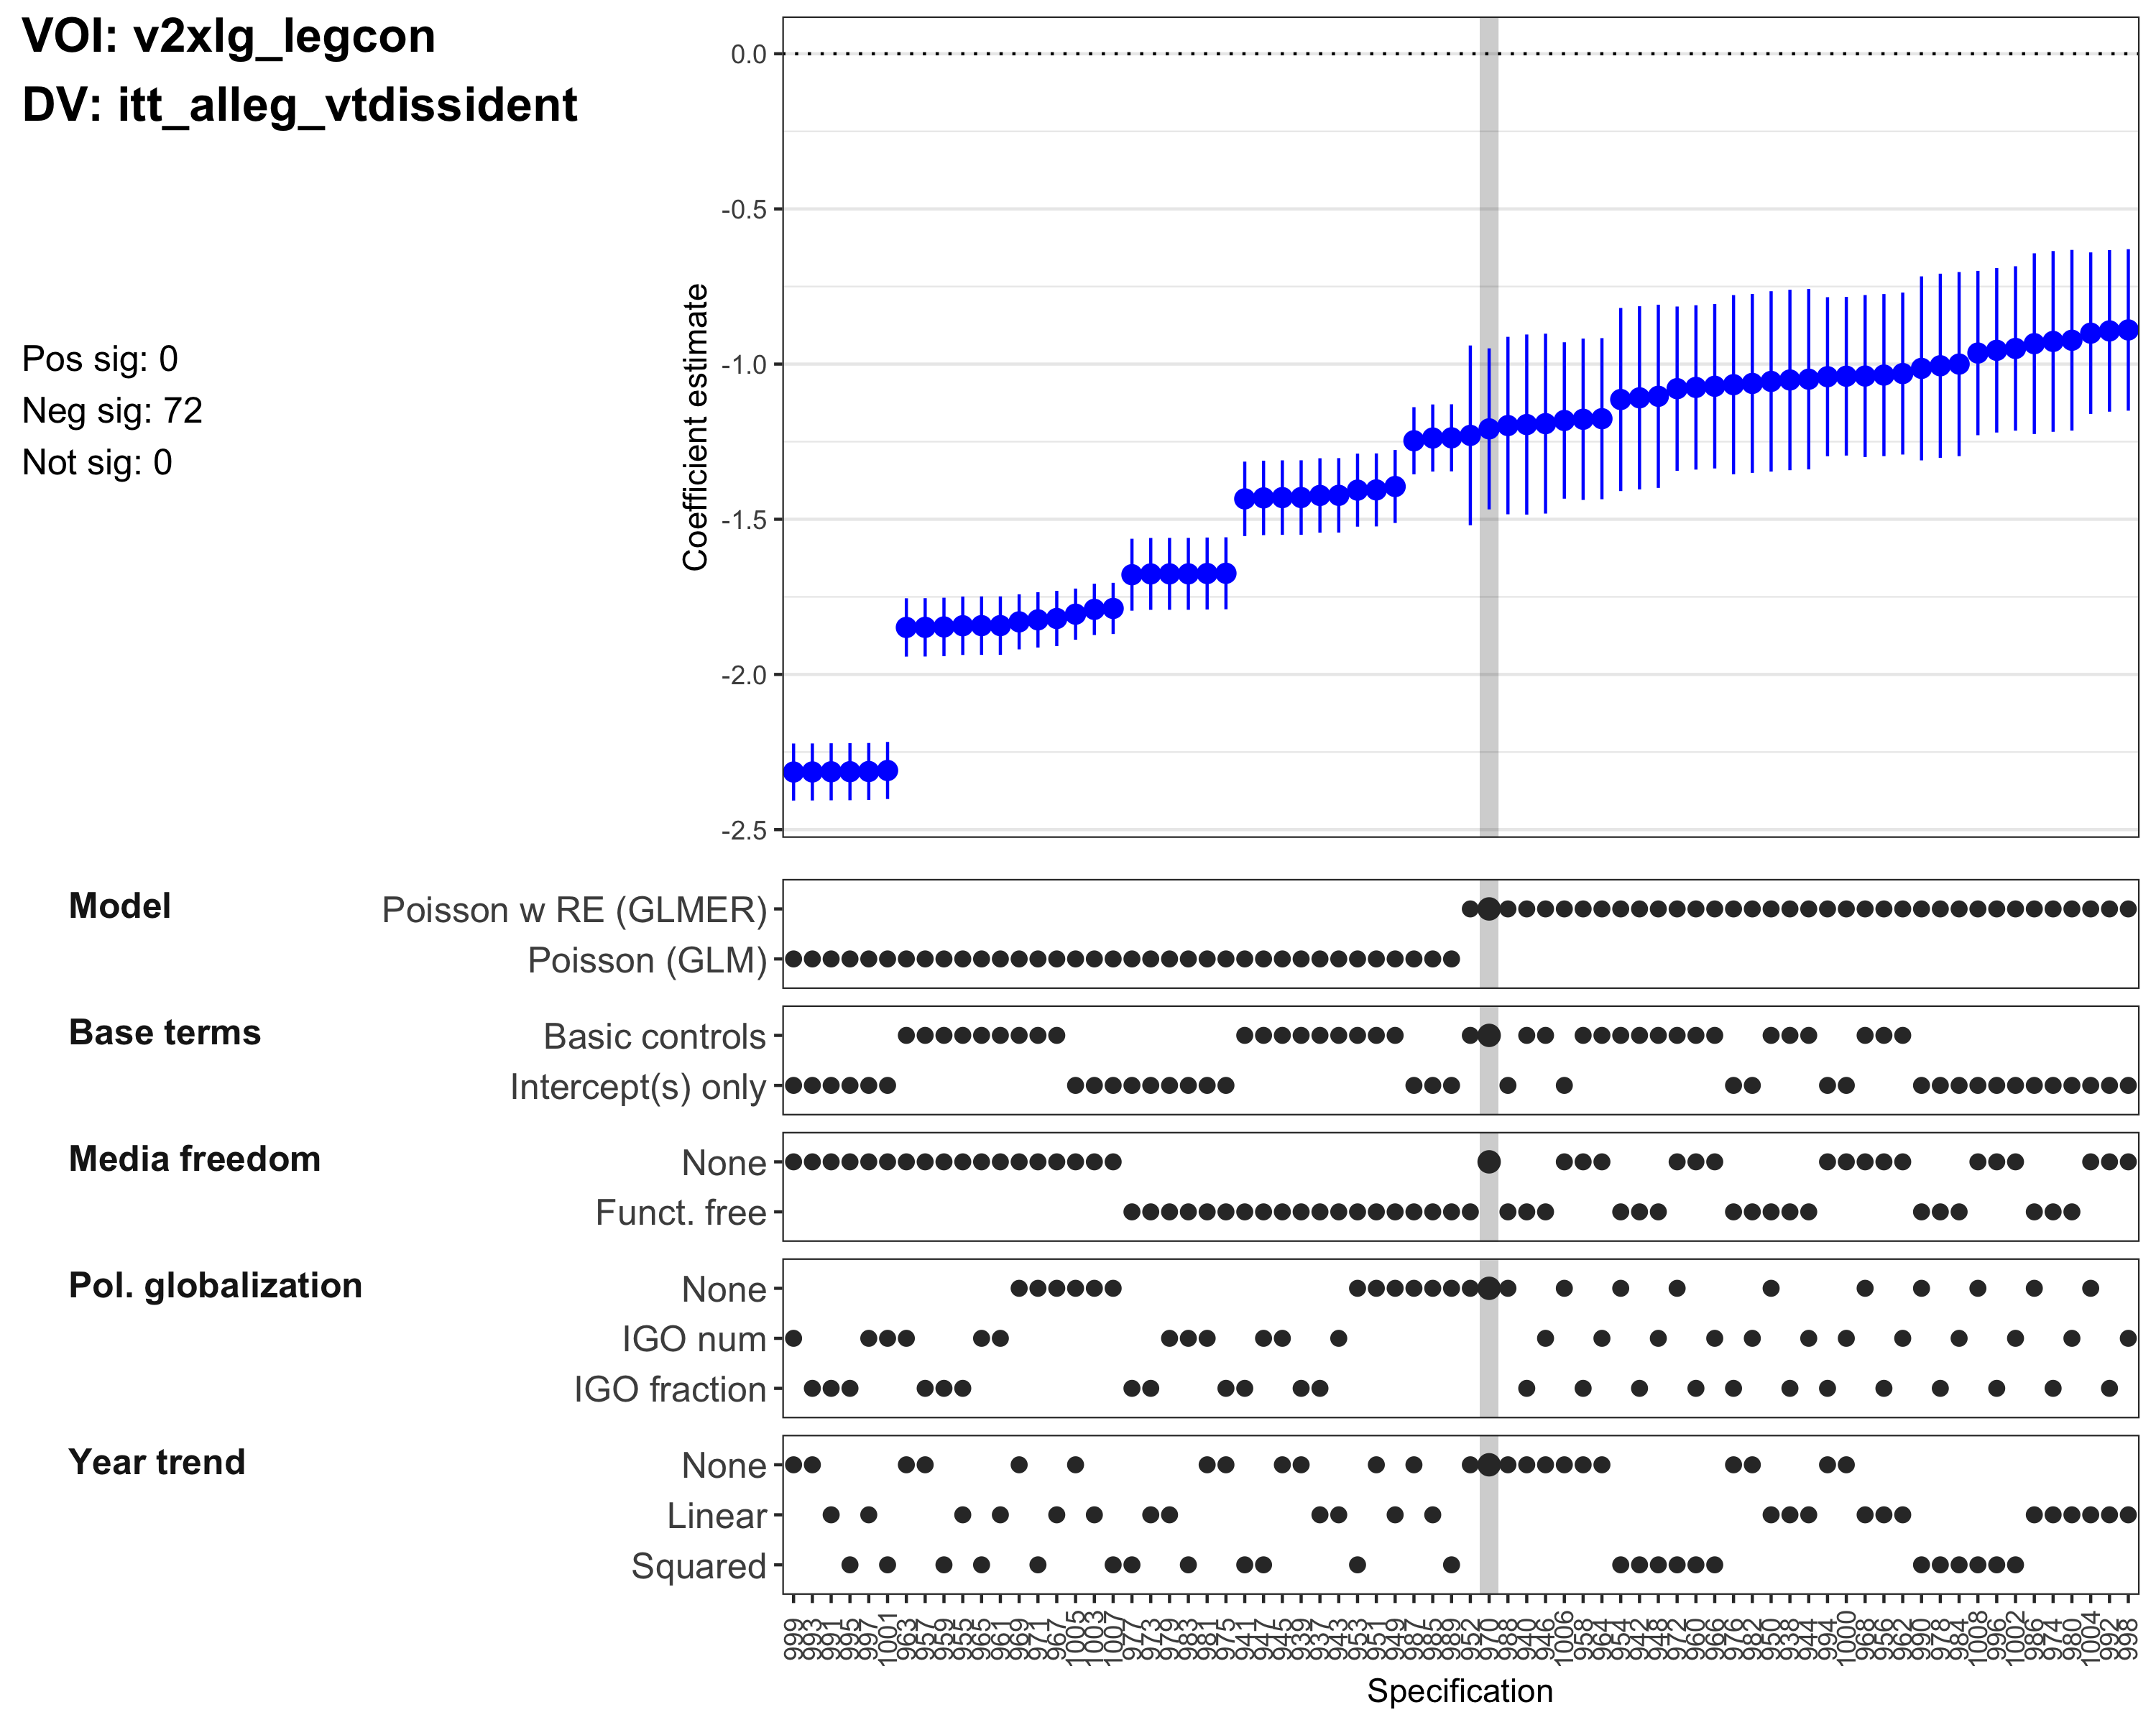
\includegraphics[height=4in]{../output/figures-robustness/specplot-v2xlg_legcon-itt_alleg_vtdissident.png}

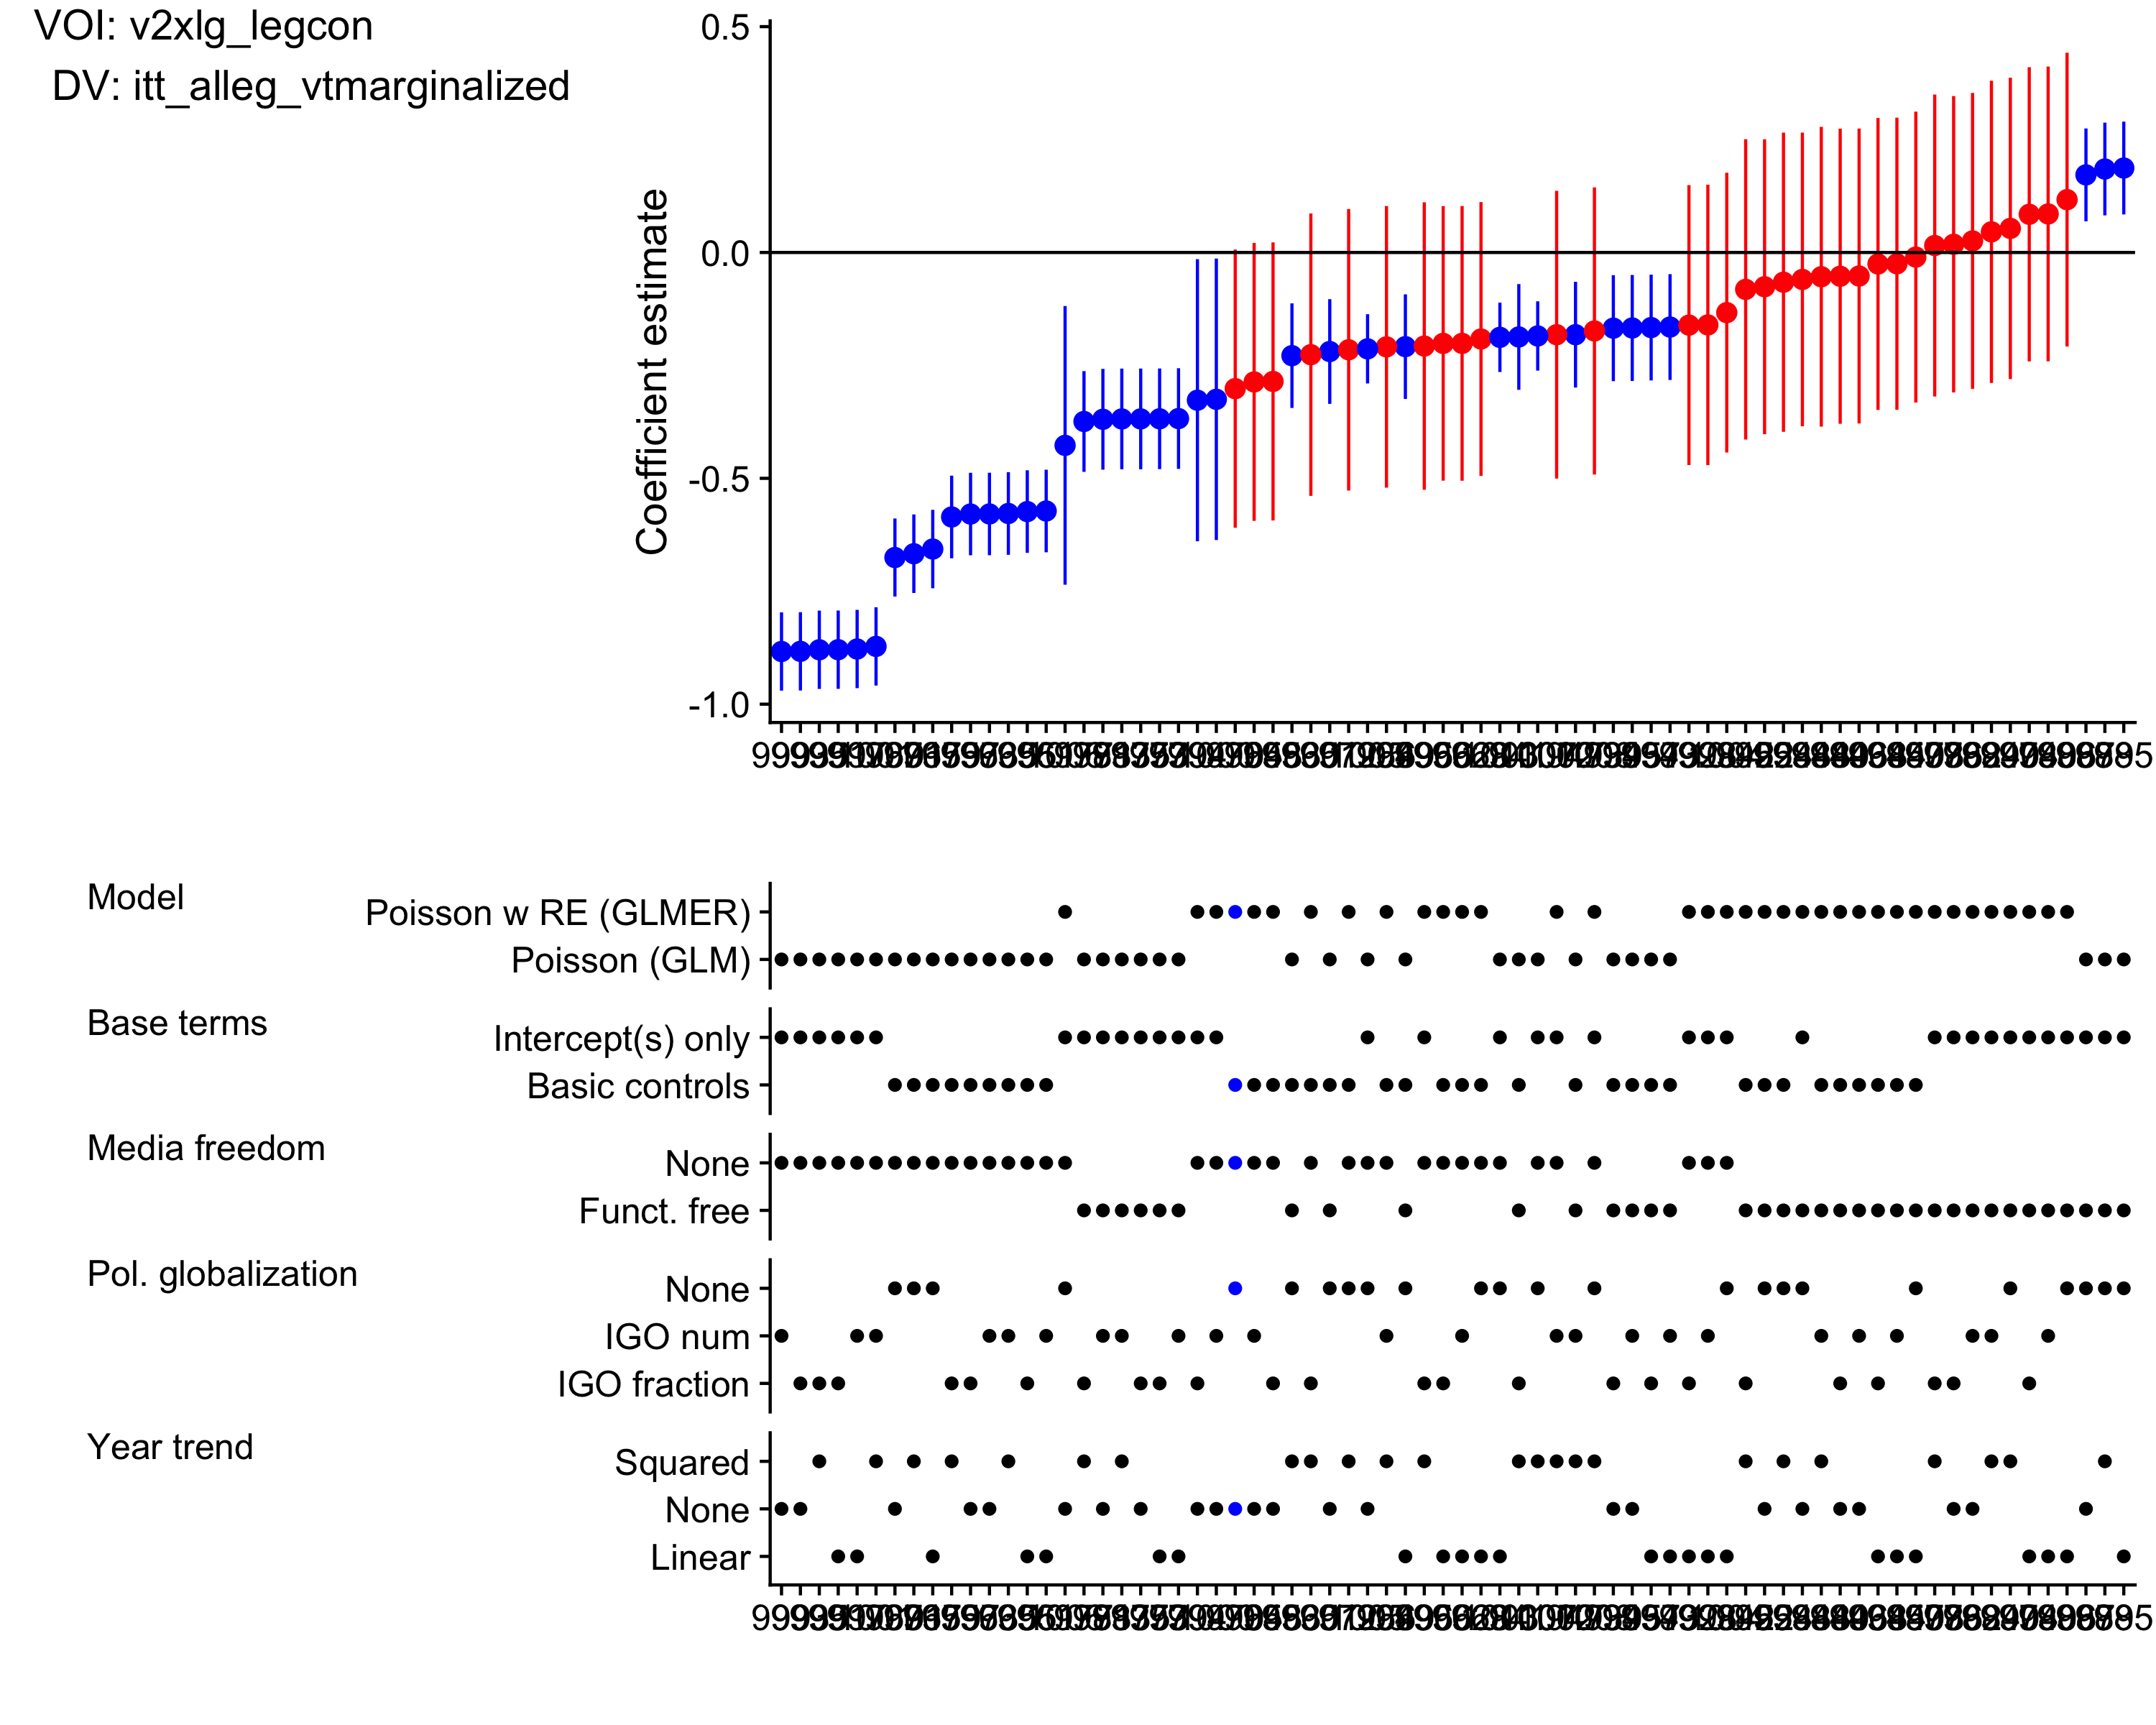
\includegraphics[height=4in]{../output/figures-robustness/specplot-v2xlg_legcon-itt_alleg_vtmarginalized.png}


\end{document}
